\chapter{Randomized low-rank approximation}
\label{chp:3-nystrom}

We go back to \refequ{equ:1-introduction-spectral-density-as-trace}, and now
directly analyze the structure of the matrix
\begin{equation}
    g_{\sigma}(t\mtx{I} - \mtx{A}).
    \label{equ:3-nystrom-matrix-function}
\end{equation}
Intuitively, because the
Gaussian \glsfirst{smoothing-kernel} \refequ{equ:1-introduction-def-gaussian-kernel}
decays rather quickly to zero, the eigenvalues of $\mtx{A}$ which lie far away
from $t$ on the spectrum will nearly vanish under the matrix function \refequ{equ:1-introduction-spectral-density-as-trace}.
What results is a matrix which is \emph{numerically low-rank}.

%%%%%%%%%%%%%%%%%%%%%%%%%%%%%%%%%%%%%%%%%%%%%%%%%%%%%%%%%%%%%%%%%%%%%%%%%%%%%%%%

\section{The numerical rank of a matrix}
\label{sec:3-nystrom-numerical-rank}

\todo{write proposition}

To account for the finite precision of floating point operations, we use the
notion of the \gls{numerical-rank} \cite[Definition~1.1]{noga2013rank}
of a matrix $\mtx{B} \in \mathbb{R}^{n \times n}$, which we define as
\begin{equation}
    r_{\varepsilon, \cdot}(\mtx{B}) = \min \{\rank(\mtx{C}): \mtx{C} \in \mathbb{R}^{n \times n}: \lVert \mtx{B} - \mtx{C} \rVert _{\cdot} \leq \varepsilon \}.
    \label{equ:3-nystrom-def-numerical-rank}
\end{equation}
A matrix is then said to be numerically low-rank, if $r_{\varepsilon, \cdot}(\mtx{B}) \ll n$.\\ 

For unitarily invariant norms $\lVert \cdot \rVert _{\cdot}$ and 
symmetric positive definite matrices $\mtx{B}$, we may use
\cite[Theorem~5]{mirsky1960truncation} to express \gls{numerical-rank} in terms
of the eigenvalues $\mu_1, \dots, \mu_n$ of $\mtx{B}$.
In particular, for the spectral norm $\lVert \cdot \rVert _2$ we have
\begin{equation}
    r_{\varepsilon, 2}(\mtx{B}) = \min \{1 \leq r \leq n: \mu_{r+1} \leq \varepsilon \},
    \label{equ:3-nystrom-numerical-rank-spectral-norm}
\end{equation}
while for the Frobenius norm $\lVert \cdot \rVert _F$ we obtain
\begin{equation}
    r_{\varepsilon, F}(\mtx{B}) = \min \{1 \leq r \leq n: \sum_{j=r+1}^n \mu_{j}^2 \leq \varepsilon^2 \}.
    \label{equ:3-nystrom-numerical-rank-frobenius-norm}
\end{equation}\\

The eigenvalues of $g_{\sigma}(t\mtx{I} - \mtx{A})$ are given by
\begin{equation}
    \mu_i(t) = g_{\sigma}(t - \lambda_{(i)}) = \frac{1}{n \sqrt{2 \pi \sigma^2}} e^{-\frac{(t - \lambda_{(i)})^2}{2 \sigma^2}}
    \label{equ:3-nystrom-kernel-function-eigenvalues}
\end{equation}
where $\lambda_{(i)}$ denote the eigenvalues of $\mtx{A}$ sorted by increasing
distance from $t$, i.e. such that $\mu_1(t) \geq \dots \geq \mu_n(t)$. Consequently,
we may upper bound the numerical rank of \refequ{equ:3-nystrom-matrix-function} as
\begin{equation}
    r_{\varepsilon, \cdot}(g_{\sigma}(t\mtx{I} - \mtx{A})) \leq \#\{1\leq i\leq n: |t - \mu_i(t)| \leq C_{\varepsilon, \cdot}(\sigma)\}
    \label{equ:3-nystrom-kernel-numerical-rank}
\end{equation}
where we define the distances
\begin{align}
    C_{\varepsilon, 2}(\sigma) = \sigma \sqrt{-2 \log(n \sqrt{2 \pi} \sigma \varepsilon)}, \label{equ:3-nystrom-kernel-numerical-rank-spectral-constant} \\
    C_{\varepsilon, F}(\sigma) = \sigma \sqrt{-2 \log(\sqrt{2 \pi} \sigma \varepsilon)}. \label{equ:3-nystrom-kernel-numerical-rank-frobenius-constant} 
\end{align}
For the spectral norm, \refequ{equ:3-nystrom-kernel-numerical-rank} even holds
as an equality.
The expression \refequ{equ:3-nystrom-kernel-numerical-rank} has a very
visual interpretation: The \glsfirst{numerical-rank} of a matrix is at most
equal to the number of eigenvalues which are closer to $t$ than $C_{\varepsilon, \cdot}(\sigma)$.
This is also illustrated in \reffig{fig:3-nystrom-numerical-rank-constant}.\\
\begin{figure}
    \centering
    \begin{tikzpicture}
    \fill[lightblue] (-2, -0.15) rectangle (1.5, 0.15);
    \draw[thick, ->] (-5, 0) to (5, 0);
    \fill[darkblue] (-4, 0) circle (0.075) node[above] {$\lambda_1$};
    \fill[darkblue] (-3, 0) circle (0.075) node[above] {$\lambda_2$};
    \fill[darkblue] (-2.4, 0) circle (0.075) node[above] {$\lambda_3$};
    \fill[darkblue] (-1, 0) circle (0.075) node[above] {$\lambda_4$};
    \fill[darkblue] (0.3, 0) circle (0.075) node[above] {$\lambda_5$};
    \fill[darkblue] (1, 0) circle (0.075) node[above] {$\lambda_6$};
    \fill[darkblue] (2.8, 0) circle (0.075) node[above] {$\lambda_7$};
    \fill[darkblue] (3.6, 0) circle (0.075) node[above] {$\lambda_8$};
    \fill[darkblue] (4, 0) circle (0.075) node[above] {$\lambda_9$};
    \draw[darkblue, ultra thick] (-0.155, 0.15) to (-0.155, -0.15) node[below] {$t$};
    \draw[darkblue, thick] (-2, 0.15) to (-2, -0.15) node[below] {$t - C_{\varepsilon, \cdot}(\sigma)$};
    \draw[darkblue, thick] (1.5, 0.15) to (1.5, -0.15) node[below] {$t + C_{\varepsilon, \cdot}(\sigma)$};
\end{tikzpicture}

    \caption{The numerical rank.}
    \label{fig:3-nystrom-numerical-rank-constant}
\end{figure}

If we additionally assume the eigenvalues of the matrix $\mtx{A}$
to be evenly distributed within $[a, b]$, i.e. in any subinterval of fixed length in
$[a, b]$ we can expect to find roughly the same number of eigenvalues (see \reffig{fig:3-nystrom-evenly-distributed-spectrum}), then
we can estimate the numerical rank of $g_{\sigma}(t\mtx{I} - \mtx{A})$ as
\begin{equation}
    r_{\varepsilon, \cdot}(g_{\sigma}(t\mtx{I} - \mtx{A})) \lessapprox \frac{2 n}{b - a} C_{\varepsilon, \cdot}(\sigma).
    \label{equ:3-nystrom-kernel-numerical-rank-even-eigenvalues}
\end{equation}

\begin{figure}
    \centering
    \begin{subfigure}[t]{0.45\columnwidth}
        \begin{tikzpicture}
    \draw[thick, ->] (-1, -1) to (5, -1)  node[above] {$t$};
    %\node[anchor=east] at (-1.5, -1) {unevenly distributed};
    \fill[darkblue] (-0.5, -1) circle (0.075);
    \fill[darkblue] (-0.1, -1) circle (0.075);
    \fill[darkblue] (0.9, -1) circle (0.075);
    \fill[darkblue] (2.15, -1) circle (0.075);
    \fill[darkblue] (2.3, -1) circle (0.075);
    \fill[darkblue] (2.5, -1) circle (0.075);
    \fill[darkblue] (2.8, -1) circle (0.075);
    \fill[darkblue] (3.6, -1) circle (0.075);
    \fill[darkblue] (4, -1) circle (0.075);
    \draw[<-] (2.5, -1.1) to (2.5, -1.4) node[below] {higher rank};
    \draw[<-] (0.2, -1.1) to (0.2, -1.4) node[below] {lower rank};
\end{tikzpicture}

        \caption{Unevenly distributed spectrum}
    \end{subfigure}
    \begin{subfigure}[t]{0.45\columnwidth}
        \begin{tikzpicture}
    \fill[white] (-1, -1.5) rectangle (5, 0.5); 
    \draw[thick, ->] (-1, 0) to (5, 0)  node[above] {$t$};
    %\node[anchor=east] at (-1.5, 0) {evenly distributed};
    \fill[darkblue] (-0.6, 0) circle (0.075);
    \fill[darkblue] (0, 0) circle (0.075);
    \fill[darkblue] (0.55, 0) circle (0.075);
    \fill[darkblue] (1.2, 0) circle (0.075);
    \fill[darkblue] (1.9, 0) circle (0.075);
    \fill[darkblue] (2.45, 0) circle (0.075);
    \fill[darkblue] (3, 0) circle (0.075);
    \fill[darkblue] (3.6, 0) circle (0.075);
    \fill[darkblue] (4.2, 0) circle (0.075);
    \node at (2.25, -0.8) {same rank everywhere};
\end{tikzpicture}

        \caption{Evenly distributed spectrum}
    \end{subfigure}      
    \caption{Examples of an evenly and unevenly distributed spectrum.}
    \label{fig:3-nystrom-evenly-distributed-spectrum}
\end{figure}

In \reffig{fig:3-nystrom-singular-value-decay}, we numerically check the decay
of the eigenvalues for one of our example matrices which we use in the numerical
experiments (\refsec{sec:5-experiments-density-function}).
\begin{figure}[ht]
    \centering
    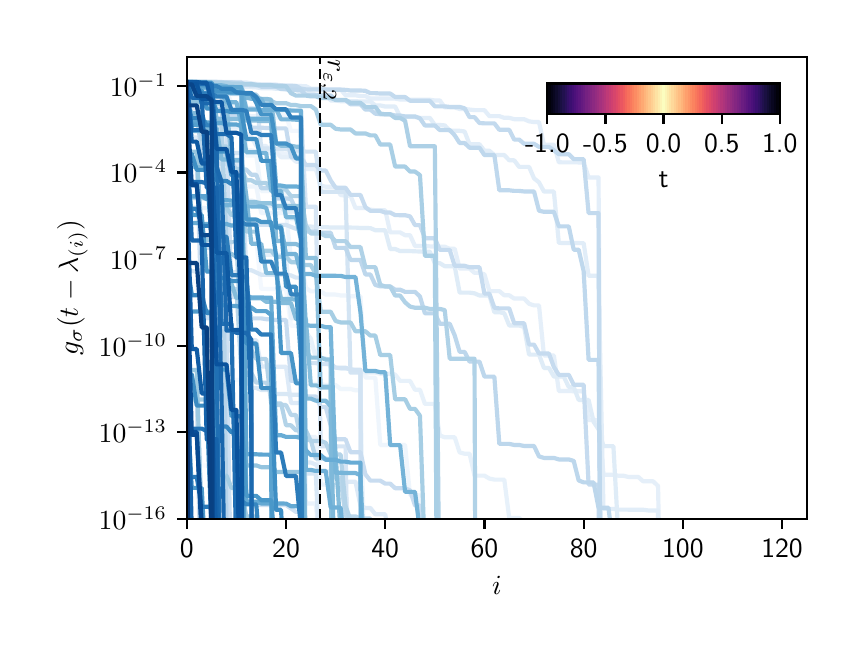
\begin{tikzpicture}
    \node at (0, 0) {%% Creator: Matplotlib, PGF backend
%%
%% To include the figure in your LaTeX document, write
%%   \input{<filename>.pgf}
%%
%% Make sure the required packages are loaded in your preamble
%%   \usepackage{pgf}
%%
%% Also ensure that all the required font packages are loaded; for instance,
%% the lmodern package is sometimes necessary when using math font.
%%   \usepackage{lmodern}
%%
%% Figures using additional raster images can only be included by \input if
%% they are in the same directory as the main LaTeX file. For loading figures
%% from other directories you can use the `import` package
%%   \usepackage{import}
%%
%% and then include the figures with
%%   \import{<path to file>}{<filename>.pgf}
%%
%% Matplotlib used the following preamble
%%   \def\mathdefault#1{#1}
%%   \everymath=\expandafter{\the\everymath\displaystyle}
%%   
%%   \usepackage{fontspec}
%%   \setmainfont{DejaVuSerif.ttf}[Path=\detokenize{C:/Users/fabio/Documents/Work/MasterThesis/Rand-SD/.venv/Lib/site-packages/matplotlib/mpl-data/fonts/ttf/}]
%%   \setsansfont{DejaVuSans.ttf}[Path=\detokenize{C:/Users/fabio/Documents/Work/MasterThesis/Rand-SD/.venv/Lib/site-packages/matplotlib/mpl-data/fonts/ttf/}]
%%   \setmonofont{DejaVuSansMono.ttf}[Path=\detokenize{C:/Users/fabio/Documents/Work/MasterThesis/Rand-SD/.venv/Lib/site-packages/matplotlib/mpl-data/fonts/ttf/}]
%%   \makeatletter\@ifpackageloaded{underscore}{}{\usepackage[strings]{underscore}}\makeatother
%%
\begingroup%
\makeatletter%
\begin{pgfpicture}%
\pgfpathrectangle{\pgfpointorigin}{\pgfqpoint{3.958241in}{2.931603in}}%
\pgfusepath{use as bounding box, clip}%
\begin{pgfscope}%
\pgfsetbuttcap%
\pgfsetmiterjoin%
\definecolor{currentfill}{rgb}{1.000000,1.000000,1.000000}%
\pgfsetfillcolor{currentfill}%
\pgfsetlinewidth{0.000000pt}%
\definecolor{currentstroke}{rgb}{1.000000,1.000000,1.000000}%
\pgfsetstrokecolor{currentstroke}%
\pgfsetdash{}{0pt}%
\pgfpathmoveto{\pgfqpoint{0.000000in}{0.000000in}}%
\pgfpathlineto{\pgfqpoint{3.958241in}{0.000000in}}%
\pgfpathlineto{\pgfqpoint{3.958241in}{2.931603in}}%
\pgfpathlineto{\pgfqpoint{0.000000in}{2.931603in}}%
\pgfpathlineto{\pgfqpoint{0.000000in}{0.000000in}}%
\pgfpathclose%
\pgfusepath{fill}%
\end{pgfscope}%
\begin{pgfscope}%
\pgfsetbuttcap%
\pgfsetmiterjoin%
\definecolor{currentfill}{rgb}{1.000000,1.000000,1.000000}%
\pgfsetfillcolor{currentfill}%
\pgfsetlinewidth{0.000000pt}%
\definecolor{currentstroke}{rgb}{0.000000,0.000000,0.000000}%
\pgfsetstrokecolor{currentstroke}%
\pgfsetstrokeopacity{0.000000}%
\pgfsetdash{}{0pt}%
\pgfpathmoveto{\pgfqpoint{0.749693in}{0.521603in}}%
\pgfpathlineto{\pgfqpoint{3.849693in}{0.521603in}}%
\pgfpathlineto{\pgfqpoint{3.849693in}{2.831603in}}%
\pgfpathlineto{\pgfqpoint{0.749693in}{2.831603in}}%
\pgfpathlineto{\pgfqpoint{0.749693in}{0.521603in}}%
\pgfpathclose%
\pgfusepath{fill}%
\end{pgfscope}%
\begin{pgfscope}%
\pgfsetbuttcap%
\pgfsetroundjoin%
\definecolor{currentfill}{rgb}{0.000000,0.000000,0.000000}%
\pgfsetfillcolor{currentfill}%
\pgfsetlinewidth{0.803000pt}%
\definecolor{currentstroke}{rgb}{0.000000,0.000000,0.000000}%
\pgfsetstrokecolor{currentstroke}%
\pgfsetdash{}{0pt}%
\pgfsys@defobject{currentmarker}{\pgfqpoint{0.000000in}{-0.048611in}}{\pgfqpoint{0.000000in}{0.000000in}}{%
\pgfpathmoveto{\pgfqpoint{0.000000in}{0.000000in}}%
\pgfpathlineto{\pgfqpoint{0.000000in}{-0.048611in}}%
\pgfusepath{stroke,fill}%
}%
\begin{pgfscope}%
\pgfsys@transformshift{0.749693in}{0.521603in}%
\pgfsys@useobject{currentmarker}{}%
\end{pgfscope}%
\end{pgfscope}%
\begin{pgfscope}%
\definecolor{textcolor}{rgb}{0.000000,0.000000,0.000000}%
\pgfsetstrokecolor{textcolor}%
\pgfsetfillcolor{textcolor}%
\pgftext[x=0.749693in,y=0.424381in,,top]{\color{textcolor}{\sffamily\fontsize{10.000000}{12.000000}\selectfont\catcode`\^=\active\def^{\ifmmode\sp\else\^{}\fi}\catcode`\%=\active\def%{\%}0}}%
\end{pgfscope}%
\begin{pgfscope}%
\pgfsetbuttcap%
\pgfsetroundjoin%
\definecolor{currentfill}{rgb}{0.000000,0.000000,0.000000}%
\pgfsetfillcolor{currentfill}%
\pgfsetlinewidth{0.803000pt}%
\definecolor{currentstroke}{rgb}{0.000000,0.000000,0.000000}%
\pgfsetstrokecolor{currentstroke}%
\pgfsetdash{}{0pt}%
\pgfsys@defobject{currentmarker}{\pgfqpoint{0.000000in}{-0.048611in}}{\pgfqpoint{0.000000in}{0.000000in}}{%
\pgfpathmoveto{\pgfqpoint{0.000000in}{0.000000in}}%
\pgfpathlineto{\pgfqpoint{0.000000in}{-0.048611in}}%
\pgfusepath{stroke,fill}%
}%
\begin{pgfscope}%
\pgfsys@transformshift{1.245693in}{0.521603in}%
\pgfsys@useobject{currentmarker}{}%
\end{pgfscope}%
\end{pgfscope}%
\begin{pgfscope}%
\definecolor{textcolor}{rgb}{0.000000,0.000000,0.000000}%
\pgfsetstrokecolor{textcolor}%
\pgfsetfillcolor{textcolor}%
\pgftext[x=1.245693in,y=0.424381in,,top]{\color{textcolor}{\sffamily\fontsize{10.000000}{12.000000}\selectfont\catcode`\^=\active\def^{\ifmmode\sp\else\^{}\fi}\catcode`\%=\active\def%{\%}20}}%
\end{pgfscope}%
\begin{pgfscope}%
\pgfsetbuttcap%
\pgfsetroundjoin%
\definecolor{currentfill}{rgb}{0.000000,0.000000,0.000000}%
\pgfsetfillcolor{currentfill}%
\pgfsetlinewidth{0.803000pt}%
\definecolor{currentstroke}{rgb}{0.000000,0.000000,0.000000}%
\pgfsetstrokecolor{currentstroke}%
\pgfsetdash{}{0pt}%
\pgfsys@defobject{currentmarker}{\pgfqpoint{0.000000in}{-0.048611in}}{\pgfqpoint{0.000000in}{0.000000in}}{%
\pgfpathmoveto{\pgfqpoint{0.000000in}{0.000000in}}%
\pgfpathlineto{\pgfqpoint{0.000000in}{-0.048611in}}%
\pgfusepath{stroke,fill}%
}%
\begin{pgfscope}%
\pgfsys@transformshift{1.741693in}{0.521603in}%
\pgfsys@useobject{currentmarker}{}%
\end{pgfscope}%
\end{pgfscope}%
\begin{pgfscope}%
\definecolor{textcolor}{rgb}{0.000000,0.000000,0.000000}%
\pgfsetstrokecolor{textcolor}%
\pgfsetfillcolor{textcolor}%
\pgftext[x=1.741693in,y=0.424381in,,top]{\color{textcolor}{\sffamily\fontsize{10.000000}{12.000000}\selectfont\catcode`\^=\active\def^{\ifmmode\sp\else\^{}\fi}\catcode`\%=\active\def%{\%}40}}%
\end{pgfscope}%
\begin{pgfscope}%
\pgfsetbuttcap%
\pgfsetroundjoin%
\definecolor{currentfill}{rgb}{0.000000,0.000000,0.000000}%
\pgfsetfillcolor{currentfill}%
\pgfsetlinewidth{0.803000pt}%
\definecolor{currentstroke}{rgb}{0.000000,0.000000,0.000000}%
\pgfsetstrokecolor{currentstroke}%
\pgfsetdash{}{0pt}%
\pgfsys@defobject{currentmarker}{\pgfqpoint{0.000000in}{-0.048611in}}{\pgfqpoint{0.000000in}{0.000000in}}{%
\pgfpathmoveto{\pgfqpoint{0.000000in}{0.000000in}}%
\pgfpathlineto{\pgfqpoint{0.000000in}{-0.048611in}}%
\pgfusepath{stroke,fill}%
}%
\begin{pgfscope}%
\pgfsys@transformshift{2.237693in}{0.521603in}%
\pgfsys@useobject{currentmarker}{}%
\end{pgfscope}%
\end{pgfscope}%
\begin{pgfscope}%
\definecolor{textcolor}{rgb}{0.000000,0.000000,0.000000}%
\pgfsetstrokecolor{textcolor}%
\pgfsetfillcolor{textcolor}%
\pgftext[x=2.237693in,y=0.424381in,,top]{\color{textcolor}{\sffamily\fontsize{10.000000}{12.000000}\selectfont\catcode`\^=\active\def^{\ifmmode\sp\else\^{}\fi}\catcode`\%=\active\def%{\%}60}}%
\end{pgfscope}%
\begin{pgfscope}%
\pgfsetbuttcap%
\pgfsetroundjoin%
\definecolor{currentfill}{rgb}{0.000000,0.000000,0.000000}%
\pgfsetfillcolor{currentfill}%
\pgfsetlinewidth{0.803000pt}%
\definecolor{currentstroke}{rgb}{0.000000,0.000000,0.000000}%
\pgfsetstrokecolor{currentstroke}%
\pgfsetdash{}{0pt}%
\pgfsys@defobject{currentmarker}{\pgfqpoint{0.000000in}{-0.048611in}}{\pgfqpoint{0.000000in}{0.000000in}}{%
\pgfpathmoveto{\pgfqpoint{0.000000in}{0.000000in}}%
\pgfpathlineto{\pgfqpoint{0.000000in}{-0.048611in}}%
\pgfusepath{stroke,fill}%
}%
\begin{pgfscope}%
\pgfsys@transformshift{2.733693in}{0.521603in}%
\pgfsys@useobject{currentmarker}{}%
\end{pgfscope}%
\end{pgfscope}%
\begin{pgfscope}%
\definecolor{textcolor}{rgb}{0.000000,0.000000,0.000000}%
\pgfsetstrokecolor{textcolor}%
\pgfsetfillcolor{textcolor}%
\pgftext[x=2.733693in,y=0.424381in,,top]{\color{textcolor}{\sffamily\fontsize{10.000000}{12.000000}\selectfont\catcode`\^=\active\def^{\ifmmode\sp\else\^{}\fi}\catcode`\%=\active\def%{\%}80}}%
\end{pgfscope}%
\begin{pgfscope}%
\pgfsetbuttcap%
\pgfsetroundjoin%
\definecolor{currentfill}{rgb}{0.000000,0.000000,0.000000}%
\pgfsetfillcolor{currentfill}%
\pgfsetlinewidth{0.803000pt}%
\definecolor{currentstroke}{rgb}{0.000000,0.000000,0.000000}%
\pgfsetstrokecolor{currentstroke}%
\pgfsetdash{}{0pt}%
\pgfsys@defobject{currentmarker}{\pgfqpoint{0.000000in}{-0.048611in}}{\pgfqpoint{0.000000in}{0.000000in}}{%
\pgfpathmoveto{\pgfqpoint{0.000000in}{0.000000in}}%
\pgfpathlineto{\pgfqpoint{0.000000in}{-0.048611in}}%
\pgfusepath{stroke,fill}%
}%
\begin{pgfscope}%
\pgfsys@transformshift{3.229693in}{0.521603in}%
\pgfsys@useobject{currentmarker}{}%
\end{pgfscope}%
\end{pgfscope}%
\begin{pgfscope}%
\definecolor{textcolor}{rgb}{0.000000,0.000000,0.000000}%
\pgfsetstrokecolor{textcolor}%
\pgfsetfillcolor{textcolor}%
\pgftext[x=3.229693in,y=0.424381in,,top]{\color{textcolor}{\sffamily\fontsize{10.000000}{12.000000}\selectfont\catcode`\^=\active\def^{\ifmmode\sp\else\^{}\fi}\catcode`\%=\active\def%{\%}100}}%
\end{pgfscope}%
\begin{pgfscope}%
\pgfsetbuttcap%
\pgfsetroundjoin%
\definecolor{currentfill}{rgb}{0.000000,0.000000,0.000000}%
\pgfsetfillcolor{currentfill}%
\pgfsetlinewidth{0.803000pt}%
\definecolor{currentstroke}{rgb}{0.000000,0.000000,0.000000}%
\pgfsetstrokecolor{currentstroke}%
\pgfsetdash{}{0pt}%
\pgfsys@defobject{currentmarker}{\pgfqpoint{0.000000in}{-0.048611in}}{\pgfqpoint{0.000000in}{0.000000in}}{%
\pgfpathmoveto{\pgfqpoint{0.000000in}{0.000000in}}%
\pgfpathlineto{\pgfqpoint{0.000000in}{-0.048611in}}%
\pgfusepath{stroke,fill}%
}%
\begin{pgfscope}%
\pgfsys@transformshift{3.725693in}{0.521603in}%
\pgfsys@useobject{currentmarker}{}%
\end{pgfscope}%
\end{pgfscope}%
\begin{pgfscope}%
\definecolor{textcolor}{rgb}{0.000000,0.000000,0.000000}%
\pgfsetstrokecolor{textcolor}%
\pgfsetfillcolor{textcolor}%
\pgftext[x=3.725693in,y=0.424381in,,top]{\color{textcolor}{\sffamily\fontsize{10.000000}{12.000000}\selectfont\catcode`\^=\active\def^{\ifmmode\sp\else\^{}\fi}\catcode`\%=\active\def%{\%}120}}%
\end{pgfscope}%
\begin{pgfscope}%
\definecolor{textcolor}{rgb}{0.000000,0.000000,0.000000}%
\pgfsetstrokecolor{textcolor}%
\pgfsetfillcolor{textcolor}%
\pgftext[x=2.299693in,y=0.234413in,,top]{\color{textcolor}{\sffamily\fontsize{10.000000}{12.000000}\selectfont\catcode`\^=\active\def^{\ifmmode\sp\else\^{}\fi}\catcode`\%=\active\def%{\%}$i$}}%
\end{pgfscope}%
\begin{pgfscope}%
\pgfsetbuttcap%
\pgfsetroundjoin%
\definecolor{currentfill}{rgb}{0.000000,0.000000,0.000000}%
\pgfsetfillcolor{currentfill}%
\pgfsetlinewidth{0.803000pt}%
\definecolor{currentstroke}{rgb}{0.000000,0.000000,0.000000}%
\pgfsetstrokecolor{currentstroke}%
\pgfsetdash{}{0pt}%
\pgfsys@defobject{currentmarker}{\pgfqpoint{-0.048611in}{0.000000in}}{\pgfqpoint{-0.000000in}{0.000000in}}{%
\pgfpathmoveto{\pgfqpoint{-0.000000in}{0.000000in}}%
\pgfpathlineto{\pgfqpoint{-0.048611in}{0.000000in}}%
\pgfusepath{stroke,fill}%
}%
\begin{pgfscope}%
\pgfsys@transformshift{0.749693in}{0.521603in}%
\pgfsys@useobject{currentmarker}{}%
\end{pgfscope}%
\end{pgfscope}%
\begin{pgfscope}%
\definecolor{textcolor}{rgb}{0.000000,0.000000,0.000000}%
\pgfsetstrokecolor{textcolor}%
\pgfsetfillcolor{textcolor}%
\pgftext[x=0.309105in, y=0.468842in, left, base]{\color{textcolor}{\sffamily\fontsize{10.000000}{12.000000}\selectfont\catcode`\^=\active\def^{\ifmmode\sp\else\^{}\fi}\catcode`\%=\active\def%{\%}$\mathdefault{10^{-16}}$}}%
\end{pgfscope}%
\begin{pgfscope}%
\pgfsetbuttcap%
\pgfsetroundjoin%
\definecolor{currentfill}{rgb}{0.000000,0.000000,0.000000}%
\pgfsetfillcolor{currentfill}%
\pgfsetlinewidth{0.803000pt}%
\definecolor{currentstroke}{rgb}{0.000000,0.000000,0.000000}%
\pgfsetstrokecolor{currentstroke}%
\pgfsetdash{}{0pt}%
\pgfsys@defobject{currentmarker}{\pgfqpoint{-0.048611in}{0.000000in}}{\pgfqpoint{-0.000000in}{0.000000in}}{%
\pgfpathmoveto{\pgfqpoint{-0.000000in}{0.000000in}}%
\pgfpathlineto{\pgfqpoint{-0.048611in}{0.000000in}}%
\pgfusepath{stroke,fill}%
}%
\begin{pgfscope}%
\pgfsys@transformshift{0.749693in}{0.954728in}%
\pgfsys@useobject{currentmarker}{}%
\end{pgfscope}%
\end{pgfscope}%
\begin{pgfscope}%
\definecolor{textcolor}{rgb}{0.000000,0.000000,0.000000}%
\pgfsetstrokecolor{textcolor}%
\pgfsetfillcolor{textcolor}%
\pgftext[x=0.309105in, y=0.901967in, left, base]{\color{textcolor}{\sffamily\fontsize{10.000000}{12.000000}\selectfont\catcode`\^=\active\def^{\ifmmode\sp\else\^{}\fi}\catcode`\%=\active\def%{\%}$\mathdefault{10^{-13}}$}}%
\end{pgfscope}%
\begin{pgfscope}%
\pgfsetbuttcap%
\pgfsetroundjoin%
\definecolor{currentfill}{rgb}{0.000000,0.000000,0.000000}%
\pgfsetfillcolor{currentfill}%
\pgfsetlinewidth{0.803000pt}%
\definecolor{currentstroke}{rgb}{0.000000,0.000000,0.000000}%
\pgfsetstrokecolor{currentstroke}%
\pgfsetdash{}{0pt}%
\pgfsys@defobject{currentmarker}{\pgfqpoint{-0.048611in}{0.000000in}}{\pgfqpoint{-0.000000in}{0.000000in}}{%
\pgfpathmoveto{\pgfqpoint{-0.000000in}{0.000000in}}%
\pgfpathlineto{\pgfqpoint{-0.048611in}{0.000000in}}%
\pgfusepath{stroke,fill}%
}%
\begin{pgfscope}%
\pgfsys@transformshift{0.749693in}{1.387853in}%
\pgfsys@useobject{currentmarker}{}%
\end{pgfscope}%
\end{pgfscope}%
\begin{pgfscope}%
\definecolor{textcolor}{rgb}{0.000000,0.000000,0.000000}%
\pgfsetstrokecolor{textcolor}%
\pgfsetfillcolor{textcolor}%
\pgftext[x=0.309105in, y=1.335092in, left, base]{\color{textcolor}{\sffamily\fontsize{10.000000}{12.000000}\selectfont\catcode`\^=\active\def^{\ifmmode\sp\else\^{}\fi}\catcode`\%=\active\def%{\%}$\mathdefault{10^{-10}}$}}%
\end{pgfscope}%
\begin{pgfscope}%
\pgfsetbuttcap%
\pgfsetroundjoin%
\definecolor{currentfill}{rgb}{0.000000,0.000000,0.000000}%
\pgfsetfillcolor{currentfill}%
\pgfsetlinewidth{0.803000pt}%
\definecolor{currentstroke}{rgb}{0.000000,0.000000,0.000000}%
\pgfsetstrokecolor{currentstroke}%
\pgfsetdash{}{0pt}%
\pgfsys@defobject{currentmarker}{\pgfqpoint{-0.048611in}{0.000000in}}{\pgfqpoint{-0.000000in}{0.000000in}}{%
\pgfpathmoveto{\pgfqpoint{-0.000000in}{0.000000in}}%
\pgfpathlineto{\pgfqpoint{-0.048611in}{0.000000in}}%
\pgfusepath{stroke,fill}%
}%
\begin{pgfscope}%
\pgfsys@transformshift{0.749693in}{1.820978in}%
\pgfsys@useobject{currentmarker}{}%
\end{pgfscope}%
\end{pgfscope}%
\begin{pgfscope}%
\definecolor{textcolor}{rgb}{0.000000,0.000000,0.000000}%
\pgfsetstrokecolor{textcolor}%
\pgfsetfillcolor{textcolor}%
\pgftext[x=0.364468in, y=1.768217in, left, base]{\color{textcolor}{\sffamily\fontsize{10.000000}{12.000000}\selectfont\catcode`\^=\active\def^{\ifmmode\sp\else\^{}\fi}\catcode`\%=\active\def%{\%}$\mathdefault{10^{-7}}$}}%
\end{pgfscope}%
\begin{pgfscope}%
\pgfsetbuttcap%
\pgfsetroundjoin%
\definecolor{currentfill}{rgb}{0.000000,0.000000,0.000000}%
\pgfsetfillcolor{currentfill}%
\pgfsetlinewidth{0.803000pt}%
\definecolor{currentstroke}{rgb}{0.000000,0.000000,0.000000}%
\pgfsetstrokecolor{currentstroke}%
\pgfsetdash{}{0pt}%
\pgfsys@defobject{currentmarker}{\pgfqpoint{-0.048611in}{0.000000in}}{\pgfqpoint{-0.000000in}{0.000000in}}{%
\pgfpathmoveto{\pgfqpoint{-0.000000in}{0.000000in}}%
\pgfpathlineto{\pgfqpoint{-0.048611in}{0.000000in}}%
\pgfusepath{stroke,fill}%
}%
\begin{pgfscope}%
\pgfsys@transformshift{0.749693in}{2.254103in}%
\pgfsys@useobject{currentmarker}{}%
\end{pgfscope}%
\end{pgfscope}%
\begin{pgfscope}%
\definecolor{textcolor}{rgb}{0.000000,0.000000,0.000000}%
\pgfsetstrokecolor{textcolor}%
\pgfsetfillcolor{textcolor}%
\pgftext[x=0.364468in, y=2.201342in, left, base]{\color{textcolor}{\sffamily\fontsize{10.000000}{12.000000}\selectfont\catcode`\^=\active\def^{\ifmmode\sp\else\^{}\fi}\catcode`\%=\active\def%{\%}$\mathdefault{10^{-4}}$}}%
\end{pgfscope}%
\begin{pgfscope}%
\pgfsetbuttcap%
\pgfsetroundjoin%
\definecolor{currentfill}{rgb}{0.000000,0.000000,0.000000}%
\pgfsetfillcolor{currentfill}%
\pgfsetlinewidth{0.803000pt}%
\definecolor{currentstroke}{rgb}{0.000000,0.000000,0.000000}%
\pgfsetstrokecolor{currentstroke}%
\pgfsetdash{}{0pt}%
\pgfsys@defobject{currentmarker}{\pgfqpoint{-0.048611in}{0.000000in}}{\pgfqpoint{-0.000000in}{0.000000in}}{%
\pgfpathmoveto{\pgfqpoint{-0.000000in}{0.000000in}}%
\pgfpathlineto{\pgfqpoint{-0.048611in}{0.000000in}}%
\pgfusepath{stroke,fill}%
}%
\begin{pgfscope}%
\pgfsys@transformshift{0.749693in}{2.687228in}%
\pgfsys@useobject{currentmarker}{}%
\end{pgfscope}%
\end{pgfscope}%
\begin{pgfscope}%
\definecolor{textcolor}{rgb}{0.000000,0.000000,0.000000}%
\pgfsetstrokecolor{textcolor}%
\pgfsetfillcolor{textcolor}%
\pgftext[x=0.364468in, y=2.634467in, left, base]{\color{textcolor}{\sffamily\fontsize{10.000000}{12.000000}\selectfont\catcode`\^=\active\def^{\ifmmode\sp\else\^{}\fi}\catcode`\%=\active\def%{\%}$\mathdefault{10^{-1}}$}}%
\end{pgfscope}%
\begin{pgfscope}%
\definecolor{textcolor}{rgb}{0.000000,0.000000,0.000000}%
\pgfsetstrokecolor{textcolor}%
\pgfsetfillcolor{textcolor}%
\pgftext[x=0.253550in,y=1.676603in,,bottom,rotate=90.000000]{\color{textcolor}{\sffamily\fontsize{10.000000}{12.000000}\selectfont\catcode`\^=\active\def^{\ifmmode\sp\else\^{}\fi}\catcode`\%=\active\def%{\%}$g_{\sigma}(t - \lambda_{(i)})$}}%
\end{pgfscope}%
\begin{pgfscope}%
\pgfpathrectangle{\pgfqpoint{0.749693in}{0.521603in}}{\pgfqpoint{3.100000in}{2.310000in}}%
\pgfusepath{clip}%
\pgfsetrectcap%
\pgfsetroundjoin%
\pgfsetlinewidth{1.505625pt}%
\definecolor{currentstroke}{rgb}{0.968627,0.984314,1.000000}%
\pgfsetstrokecolor{currentstroke}%
\pgfsetdash{}{0pt}%
\pgfpathmoveto{\pgfqpoint{0.749693in}{0.980593in}}%
\pgfpathlineto{\pgfqpoint{0.799293in}{0.980290in}}%
\pgfpathlineto{\pgfqpoint{0.824093in}{0.788421in}}%
\pgfpathlineto{\pgfqpoint{0.948093in}{0.788386in}}%
\pgfpathlineto{\pgfqpoint{0.968223in}{0.511603in}}%
\pgfpathlineto{\pgfqpoint{0.968223in}{0.511603in}}%
\pgfusepath{stroke}%
\end{pgfscope}%
\begin{pgfscope}%
\pgfpathrectangle{\pgfqpoint{0.749693in}{0.521603in}}{\pgfqpoint{3.100000in}{2.310000in}}%
\pgfusepath{clip}%
\pgfsetrectcap%
\pgfsetroundjoin%
\pgfsetlinewidth{1.505625pt}%
\definecolor{currentstroke}{rgb}{0.962476,0.980377,0.998032}%
\pgfsetstrokecolor{currentstroke}%
\pgfsetdash{}{0pt}%
\pgfpathmoveto{\pgfqpoint{0.749693in}{1.709115in}}%
\pgfpathlineto{\pgfqpoint{0.799293in}{1.708387in}}%
\pgfpathlineto{\pgfqpoint{0.824093in}{1.520385in}}%
\pgfpathlineto{\pgfqpoint{0.948093in}{1.520345in}}%
\pgfpathlineto{\pgfqpoint{0.972893in}{1.217082in}}%
\pgfpathlineto{\pgfqpoint{1.022493in}{1.216187in}}%
\pgfpathlineto{\pgfqpoint{1.045763in}{0.511603in}}%
\pgfpathlineto{\pgfqpoint{1.045763in}{0.511603in}}%
\pgfusepath{stroke}%
\end{pgfscope}%
\begin{pgfscope}%
\pgfpathrectangle{\pgfqpoint{0.749693in}{0.521603in}}{\pgfqpoint{3.100000in}{2.310000in}}%
\pgfusepath{clip}%
\pgfsetrectcap%
\pgfsetroundjoin%
\pgfsetlinewidth{1.505625pt}%
\definecolor{currentstroke}{rgb}{0.953249,0.974471,0.995079}%
\pgfsetstrokecolor{currentstroke}%
\pgfsetdash{}{0pt}%
\pgfpathmoveto{\pgfqpoint{0.749693in}{2.554702in}}%
\pgfpathlineto{\pgfqpoint{0.799293in}{2.554418in}}%
\pgfpathlineto{\pgfqpoint{0.824093in}{2.476100in}}%
\pgfpathlineto{\pgfqpoint{0.948093in}{2.476083in}}%
\pgfpathlineto{\pgfqpoint{0.972893in}{2.332790in}}%
\pgfpathlineto{\pgfqpoint{1.022493in}{2.332341in}}%
\pgfpathlineto{\pgfqpoint{1.047293in}{1.918026in}}%
\pgfpathlineto{\pgfqpoint{1.096893in}{1.918026in}}%
\pgfpathlineto{\pgfqpoint{1.121693in}{1.671646in}}%
\pgfpathlineto{\pgfqpoint{1.245693in}{1.670905in}}%
\pgfpathlineto{\pgfqpoint{1.270493in}{1.487623in}}%
\pgfpathlineto{\pgfqpoint{1.320093in}{1.487623in}}%
\pgfpathlineto{\pgfqpoint{1.325178in}{0.511603in}}%
\pgfpathlineto{\pgfqpoint{1.325178in}{0.511603in}}%
\pgfusepath{stroke}%
\end{pgfscope}%
\begin{pgfscope}%
\pgfpathrectangle{\pgfqpoint{0.749693in}{0.521603in}}{\pgfqpoint{3.100000in}{2.310000in}}%
\pgfusepath{clip}%
\pgfsetrectcap%
\pgfsetroundjoin%
\pgfsetlinewidth{1.505625pt}%
\definecolor{currentstroke}{rgb}{0.947097,0.970534,0.993110}%
\pgfsetstrokecolor{currentstroke}%
\pgfsetdash{}{0pt}%
\pgfpathmoveto{\pgfqpoint{0.749693in}{2.706444in}}%
\pgfpathlineto{\pgfqpoint{0.799293in}{2.706442in}}%
\pgfpathlineto{\pgfqpoint{0.824093in}{2.689767in}}%
\pgfpathlineto{\pgfqpoint{0.948093in}{2.689762in}}%
\pgfpathlineto{\pgfqpoint{0.972893in}{2.658396in}}%
\pgfpathlineto{\pgfqpoint{1.022493in}{2.658236in}}%
\pgfpathlineto{\pgfqpoint{1.047293in}{2.628712in}}%
\pgfpathlineto{\pgfqpoint{1.096893in}{2.628712in}}%
\pgfpathlineto{\pgfqpoint{1.121693in}{2.539876in}}%
\pgfpathlineto{\pgfqpoint{1.245693in}{2.539578in}}%
\pgfpathlineto{\pgfqpoint{1.270493in}{2.461537in}}%
\pgfpathlineto{\pgfqpoint{1.320093in}{2.461537in}}%
\pgfpathlineto{\pgfqpoint{1.335563in}{0.511603in}}%
\pgfpathlineto{\pgfqpoint{1.335563in}{0.511603in}}%
\pgfusepath{stroke}%
\end{pgfscope}%
\begin{pgfscope}%
\pgfpathrectangle{\pgfqpoint{0.749693in}{0.521603in}}{\pgfqpoint{3.100000in}{2.310000in}}%
\pgfusepath{clip}%
\pgfsetrectcap%
\pgfsetroundjoin%
\pgfsetlinewidth{1.505625pt}%
\definecolor{currentstroke}{rgb}{0.937870,0.964629,0.990158}%
\pgfsetstrokecolor{currentstroke}%
\pgfsetdash{}{0pt}%
\pgfpathmoveto{\pgfqpoint{0.749693in}{2.693399in}}%
\pgfpathlineto{\pgfqpoint{0.799293in}{2.693399in}}%
\pgfpathlineto{\pgfqpoint{0.824093in}{2.666199in}}%
\pgfpathlineto{\pgfqpoint{0.948093in}{2.666052in}}%
\pgfpathlineto{\pgfqpoint{0.972893in}{2.597345in}}%
\pgfpathlineto{\pgfqpoint{1.022493in}{2.597345in}}%
\pgfpathlineto{\pgfqpoint{1.047293in}{2.338490in}}%
\pgfpathlineto{\pgfqpoint{1.096893in}{2.338045in}}%
\pgfpathlineto{\pgfqpoint{1.121693in}{2.161398in}}%
\pgfpathlineto{\pgfqpoint{1.245693in}{2.161371in}}%
\pgfpathlineto{\pgfqpoint{1.270493in}{2.020320in}}%
\pgfpathlineto{\pgfqpoint{1.320093in}{2.019716in}}%
\pgfpathlineto{\pgfqpoint{1.344893in}{1.201349in}}%
\pgfpathlineto{\pgfqpoint{1.369693in}{1.196889in}}%
\pgfpathlineto{\pgfqpoint{1.419293in}{1.196889in}}%
\pgfpathlineto{\pgfqpoint{1.444093in}{1.191212in}}%
\pgfpathlineto{\pgfqpoint{1.493693in}{1.191212in}}%
\pgfpathlineto{\pgfqpoint{1.518493in}{1.171097in}}%
\pgfpathlineto{\pgfqpoint{1.568093in}{1.171097in}}%
\pgfpathlineto{\pgfqpoint{1.592893in}{1.164460in}}%
\pgfpathlineto{\pgfqpoint{1.617693in}{1.164460in}}%
\pgfpathlineto{\pgfqpoint{1.632460in}{0.511603in}}%
\pgfpathlineto{\pgfqpoint{1.632460in}{0.511603in}}%
\pgfusepath{stroke}%
\end{pgfscope}%
\begin{pgfscope}%
\pgfpathrectangle{\pgfqpoint{0.749693in}{0.521603in}}{\pgfqpoint{3.100000in}{2.310000in}}%
\pgfusepath{clip}%
\pgfsetrectcap%
\pgfsetroundjoin%
\pgfsetlinewidth{1.505625pt}%
\definecolor{currentstroke}{rgb}{0.931719,0.960692,0.988189}%
\pgfsetstrokecolor{currentstroke}%
\pgfsetdash{}{0pt}%
\pgfpathmoveto{\pgfqpoint{0.749693in}{2.324888in}}%
\pgfpathlineto{\pgfqpoint{0.774493in}{2.322641in}}%
\pgfpathlineto{\pgfqpoint{0.824093in}{2.322641in}}%
\pgfpathlineto{\pgfqpoint{0.848893in}{2.319776in}}%
\pgfpathlineto{\pgfqpoint{0.898493in}{2.319776in}}%
\pgfpathlineto{\pgfqpoint{0.923293in}{2.309582in}}%
\pgfpathlineto{\pgfqpoint{0.972893in}{2.309582in}}%
\pgfpathlineto{\pgfqpoint{0.997693in}{2.306204in}}%
\pgfpathlineto{\pgfqpoint{1.022493in}{2.306204in}}%
\pgfpathlineto{\pgfqpoint{1.047293in}{2.183207in}}%
\pgfpathlineto{\pgfqpoint{1.096893in}{2.183207in}}%
\pgfpathlineto{\pgfqpoint{1.121693in}{2.050766in}}%
\pgfpathlineto{\pgfqpoint{1.245693in}{2.050176in}}%
\pgfpathlineto{\pgfqpoint{1.270493in}{1.823925in}}%
\pgfpathlineto{\pgfqpoint{1.320093in}{1.823925in}}%
\pgfpathlineto{\pgfqpoint{1.344893in}{1.675860in}}%
\pgfpathlineto{\pgfqpoint{1.369693in}{1.659130in}}%
\pgfpathlineto{\pgfqpoint{1.419293in}{1.659130in}}%
\pgfpathlineto{\pgfqpoint{1.444093in}{1.643181in}}%
\pgfpathlineto{\pgfqpoint{1.493693in}{1.643181in}}%
\pgfpathlineto{\pgfqpoint{1.518493in}{1.638771in}}%
\pgfpathlineto{\pgfqpoint{1.543293in}{1.638771in}}%
\pgfpathlineto{\pgfqpoint{1.568093in}{1.635204in}}%
\pgfpathlineto{\pgfqpoint{1.617693in}{1.635204in}}%
\pgfpathlineto{\pgfqpoint{1.642493in}{1.228484in}}%
\pgfpathlineto{\pgfqpoint{1.692093in}{1.227592in}}%
\pgfpathlineto{\pgfqpoint{1.716893in}{0.890977in}}%
\pgfpathlineto{\pgfqpoint{1.840893in}{0.890927in}}%
\pgfpathlineto{\pgfqpoint{1.865693in}{0.640192in}}%
\pgfpathlineto{\pgfqpoint{1.915293in}{0.639144in}}%
\pgfpathlineto{\pgfqpoint{1.915917in}{0.511603in}}%
\pgfpathlineto{\pgfqpoint{1.915917in}{0.511603in}}%
\pgfusepath{stroke}%
\end{pgfscope}%
\begin{pgfscope}%
\pgfpathrectangle{\pgfqpoint{0.749693in}{0.521603in}}{\pgfqpoint{3.100000in}{2.310000in}}%
\pgfusepath{clip}%
\pgfsetrectcap%
\pgfsetroundjoin%
\pgfsetlinewidth{1.505625pt}%
\definecolor{currentstroke}{rgb}{0.922491,0.954787,0.985236}%
\pgfsetstrokecolor{currentstroke}%
\pgfsetdash{}{0pt}%
\pgfpathmoveto{\pgfqpoint{0.749693in}{2.706374in}}%
\pgfpathlineto{\pgfqpoint{1.022493in}{2.705895in}}%
\pgfpathlineto{\pgfqpoint{1.047293in}{2.541564in}}%
\pgfpathlineto{\pgfqpoint{1.072093in}{2.534832in}}%
\pgfpathlineto{\pgfqpoint{1.121693in}{2.534832in}}%
\pgfpathlineto{\pgfqpoint{1.146493in}{2.528340in}}%
\pgfpathlineto{\pgfqpoint{1.196093in}{2.528340in}}%
\pgfpathlineto{\pgfqpoint{1.220893in}{2.526532in}}%
\pgfpathlineto{\pgfqpoint{1.245693in}{2.526532in}}%
\pgfpathlineto{\pgfqpoint{1.270493in}{2.525066in}}%
\pgfpathlineto{\pgfqpoint{1.320093in}{2.525066in}}%
\pgfpathlineto{\pgfqpoint{1.344893in}{0.930962in}}%
\pgfpathlineto{\pgfqpoint{1.394493in}{0.930962in}}%
\pgfpathlineto{\pgfqpoint{1.419293in}{0.693281in}}%
\pgfpathlineto{\pgfqpoint{1.543293in}{0.692246in}}%
\pgfpathlineto{\pgfqpoint{1.554965in}{0.511603in}}%
\pgfpathlineto{\pgfqpoint{1.554965in}{0.511603in}}%
\pgfusepath{stroke}%
\end{pgfscope}%
\begin{pgfscope}%
\pgfpathrectangle{\pgfqpoint{0.749693in}{0.521603in}}{\pgfqpoint{3.100000in}{2.310000in}}%
\pgfusepath{clip}%
\pgfsetrectcap%
\pgfsetroundjoin%
\pgfsetlinewidth{1.505625pt}%
\definecolor{currentstroke}{rgb}{0.916340,0.950850,0.983268}%
\pgfsetstrokecolor{currentstroke}%
\pgfsetdash{}{0pt}%
\pgfpathmoveto{\pgfqpoint{0.749693in}{2.672875in}}%
\pgfpathlineto{\pgfqpoint{0.848893in}{2.672240in}}%
\pgfpathlineto{\pgfqpoint{0.898493in}{2.671445in}}%
\pgfpathlineto{\pgfqpoint{0.923293in}{2.671445in}}%
\pgfpathlineto{\pgfqpoint{0.948093in}{2.668480in}}%
\pgfpathlineto{\pgfqpoint{0.997693in}{2.668480in}}%
\pgfpathlineto{\pgfqpoint{1.022493in}{2.665215in}}%
\pgfpathlineto{\pgfqpoint{1.047293in}{2.363532in}}%
\pgfpathlineto{\pgfqpoint{1.072093in}{2.363532in}}%
\pgfpathlineto{\pgfqpoint{1.096893in}{2.360392in}}%
\pgfpathlineto{\pgfqpoint{1.146493in}{2.360392in}}%
\pgfpathlineto{\pgfqpoint{1.171293in}{2.350744in}}%
\pgfpathlineto{\pgfqpoint{1.220893in}{2.350744in}}%
\pgfpathlineto{\pgfqpoint{1.245693in}{2.347986in}}%
\pgfpathlineto{\pgfqpoint{1.295293in}{2.347986in}}%
\pgfpathlineto{\pgfqpoint{1.320093in}{2.345807in}}%
\pgfpathlineto{\pgfqpoint{1.344893in}{0.598521in}}%
\pgfpathlineto{\pgfqpoint{1.394493in}{0.598521in}}%
\pgfpathlineto{\pgfqpoint{1.402792in}{0.511603in}}%
\pgfpathlineto{\pgfqpoint{1.402792in}{0.511603in}}%
\pgfusepath{stroke}%
\end{pgfscope}%
\begin{pgfscope}%
\pgfpathrectangle{\pgfqpoint{0.749693in}{0.521603in}}{\pgfqpoint{3.100000in}{2.310000in}}%
\pgfusepath{clip}%
\pgfsetrectcap%
\pgfsetroundjoin%
\pgfsetlinewidth{1.505625pt}%
\definecolor{currentstroke}{rgb}{0.907113,0.944944,0.980315}%
\pgfsetstrokecolor{currentstroke}%
\pgfsetdash{}{0pt}%
\pgfpathmoveto{\pgfqpoint{0.749693in}{2.078631in}}%
\pgfpathlineto{\pgfqpoint{0.799293in}{2.078631in}}%
\pgfpathlineto{\pgfqpoint{0.824093in}{2.075895in}}%
\pgfpathlineto{\pgfqpoint{0.848893in}{2.075895in}}%
\pgfpathlineto{\pgfqpoint{0.873693in}{2.072498in}}%
\pgfpathlineto{\pgfqpoint{0.923293in}{2.072498in}}%
\pgfpathlineto{\pgfqpoint{0.948093in}{2.060076in}}%
\pgfpathlineto{\pgfqpoint{0.997693in}{2.060076in}}%
\pgfpathlineto{\pgfqpoint{1.022493in}{2.046813in}}%
\pgfpathlineto{\pgfqpoint{1.047293in}{1.996220in}}%
\pgfpathlineto{\pgfqpoint{1.096893in}{1.996220in}}%
\pgfpathlineto{\pgfqpoint{1.121693in}{1.842290in}}%
\pgfpathlineto{\pgfqpoint{1.171293in}{1.842290in}}%
\pgfpathlineto{\pgfqpoint{1.196093in}{1.841153in}}%
\pgfpathlineto{\pgfqpoint{1.245693in}{1.841153in}}%
\pgfpathlineto{\pgfqpoint{1.270493in}{1.524894in}}%
\pgfpathlineto{\pgfqpoint{1.320093in}{1.524894in}}%
\pgfpathlineto{\pgfqpoint{1.344893in}{1.455081in}}%
\pgfpathlineto{\pgfqpoint{1.369693in}{1.422826in}}%
\pgfpathlineto{\pgfqpoint{1.394493in}{1.324634in}}%
\pgfpathlineto{\pgfqpoint{1.444093in}{1.324634in}}%
\pgfpathlineto{\pgfqpoint{1.468893in}{1.279117in}}%
\pgfpathlineto{\pgfqpoint{1.493693in}{1.279117in}}%
\pgfpathlineto{\pgfqpoint{1.518493in}{1.272717in}}%
\pgfpathlineto{\pgfqpoint{1.568093in}{1.272717in}}%
\pgfpathlineto{\pgfqpoint{1.592893in}{1.263404in}}%
\pgfpathlineto{\pgfqpoint{1.617693in}{1.263404in}}%
\pgfpathlineto{\pgfqpoint{1.642493in}{1.253149in}}%
\pgfpathlineto{\pgfqpoint{1.692093in}{1.253149in}}%
\pgfpathlineto{\pgfqpoint{1.716893in}{1.247579in}}%
\pgfpathlineto{\pgfqpoint{1.766493in}{1.247579in}}%
\pgfpathlineto{\pgfqpoint{1.791293in}{1.243187in}}%
\pgfpathlineto{\pgfqpoint{1.816093in}{1.211530in}}%
\pgfpathlineto{\pgfqpoint{1.865693in}{1.211530in}}%
\pgfpathlineto{\pgfqpoint{1.890493in}{1.167261in}}%
\pgfpathlineto{\pgfqpoint{1.915293in}{1.167261in}}%
\pgfpathlineto{\pgfqpoint{1.940093in}{1.096592in}}%
\pgfpathlineto{\pgfqpoint{1.989693in}{1.096592in}}%
\pgfpathlineto{\pgfqpoint{2.014493in}{0.938712in}}%
\pgfpathlineto{\pgfqpoint{2.039293in}{0.929730in}}%
\pgfpathlineto{\pgfqpoint{2.088893in}{0.929730in}}%
\pgfpathlineto{\pgfqpoint{2.113693in}{0.853871in}}%
\pgfpathlineto{\pgfqpoint{2.138493in}{0.847608in}}%
\pgfpathlineto{\pgfqpoint{2.163293in}{0.847608in}}%
\pgfpathlineto{\pgfqpoint{2.188093in}{0.737866in}}%
\pgfpathlineto{\pgfqpoint{2.237693in}{0.737866in}}%
\pgfpathlineto{\pgfqpoint{2.262493in}{0.723060in}}%
\pgfpathlineto{\pgfqpoint{2.287293in}{0.718168in}}%
\pgfpathlineto{\pgfqpoint{2.336893in}{0.718168in}}%
\pgfpathlineto{\pgfqpoint{2.361693in}{0.526213in}}%
\pgfpathlineto{\pgfqpoint{2.411293in}{0.526213in}}%
\pgfpathlineto{\pgfqpoint{2.426649in}{0.511603in}}%
\pgfpathlineto{\pgfqpoint{2.426649in}{0.511603in}}%
\pgfusepath{stroke}%
\end{pgfscope}%
\begin{pgfscope}%
\pgfpathrectangle{\pgfqpoint{0.749693in}{0.521603in}}{\pgfqpoint{3.100000in}{2.310000in}}%
\pgfusepath{clip}%
\pgfsetrectcap%
\pgfsetroundjoin%
\pgfsetlinewidth{1.505625pt}%
\definecolor{currentstroke}{rgb}{0.897885,0.939039,0.977363}%
\pgfsetstrokecolor{currentstroke}%
\pgfsetdash{}{0pt}%
\pgfpathmoveto{\pgfqpoint{0.749693in}{2.651865in}}%
\pgfpathlineto{\pgfqpoint{0.799293in}{2.651865in}}%
\pgfpathlineto{\pgfqpoint{0.824093in}{2.603740in}}%
\pgfpathlineto{\pgfqpoint{0.948093in}{2.603347in}}%
\pgfpathlineto{\pgfqpoint{0.972893in}{2.478085in}}%
\pgfpathlineto{\pgfqpoint{1.022493in}{2.478085in}}%
\pgfpathlineto{\pgfqpoint{1.047293in}{2.446832in}}%
\pgfpathlineto{\pgfqpoint{1.072093in}{2.432028in}}%
\pgfpathlineto{\pgfqpoint{1.096893in}{2.385655in}}%
\pgfpathlineto{\pgfqpoint{1.146493in}{2.385655in}}%
\pgfpathlineto{\pgfqpoint{1.171293in}{2.355809in}}%
\pgfpathlineto{\pgfqpoint{1.196093in}{2.355809in}}%
\pgfpathlineto{\pgfqpoint{1.220893in}{2.330006in}}%
\pgfpathlineto{\pgfqpoint{1.270493in}{2.330006in}}%
\pgfpathlineto{\pgfqpoint{1.295293in}{2.307630in}}%
\pgfpathlineto{\pgfqpoint{1.320093in}{2.307630in}}%
\pgfpathlineto{\pgfqpoint{1.344893in}{2.271269in}}%
\pgfpathlineto{\pgfqpoint{1.394493in}{2.271269in}}%
\pgfpathlineto{\pgfqpoint{1.419293in}{2.187410in}}%
\pgfpathlineto{\pgfqpoint{1.444093in}{2.182538in}}%
\pgfpathlineto{\pgfqpoint{1.493693in}{2.182538in}}%
\pgfpathlineto{\pgfqpoint{1.518493in}{2.140982in}}%
\pgfpathlineto{\pgfqpoint{1.543293in}{2.137520in}}%
\pgfpathlineto{\pgfqpoint{1.568093in}{2.137520in}}%
\pgfpathlineto{\pgfqpoint{1.592893in}{2.076104in}}%
\pgfpathlineto{\pgfqpoint{1.642493in}{2.076104in}}%
\pgfpathlineto{\pgfqpoint{1.667293in}{2.067714in}}%
\pgfpathlineto{\pgfqpoint{1.692093in}{2.064936in}}%
\pgfpathlineto{\pgfqpoint{1.741693in}{2.064936in}}%
\pgfpathlineto{\pgfqpoint{1.766493in}{1.953992in}}%
\pgfpathlineto{\pgfqpoint{1.816093in}{1.953992in}}%
\pgfpathlineto{\pgfqpoint{1.840893in}{1.940104in}}%
\pgfpathlineto{\pgfqpoint{1.865693in}{1.940104in}}%
\pgfpathlineto{\pgfqpoint{1.890493in}{1.885857in}}%
\pgfpathlineto{\pgfqpoint{1.940093in}{1.885857in}}%
\pgfpathlineto{\pgfqpoint{1.989693in}{1.882489in}}%
\pgfpathlineto{\pgfqpoint{2.039293in}{1.882489in}}%
\pgfpathlineto{\pgfqpoint{2.064093in}{1.872065in}}%
\pgfpathlineto{\pgfqpoint{2.088893in}{1.872065in}}%
\pgfpathlineto{\pgfqpoint{2.113693in}{1.773056in}}%
\pgfpathlineto{\pgfqpoint{2.163293in}{1.773056in}}%
\pgfpathlineto{\pgfqpoint{2.188093in}{1.751946in}}%
\pgfpathlineto{\pgfqpoint{2.212893in}{1.751946in}}%
\pgfpathlineto{\pgfqpoint{2.237693in}{1.744421in}}%
\pgfpathlineto{\pgfqpoint{2.262493in}{1.660597in}}%
\pgfpathlineto{\pgfqpoint{2.312093in}{1.660597in}}%
\pgfpathlineto{\pgfqpoint{2.336893in}{1.639657in}}%
\pgfpathlineto{\pgfqpoint{2.361693in}{1.639657in}}%
\pgfpathlineto{\pgfqpoint{2.386493in}{1.623234in}}%
\pgfpathlineto{\pgfqpoint{2.436093in}{1.623234in}}%
\pgfpathlineto{\pgfqpoint{2.460893in}{1.597133in}}%
\pgfpathlineto{\pgfqpoint{2.485693in}{1.589179in}}%
\pgfpathlineto{\pgfqpoint{2.510493in}{1.589179in}}%
\pgfpathlineto{\pgfqpoint{2.535293in}{1.338681in}}%
\pgfpathlineto{\pgfqpoint{2.584893in}{1.338681in}}%
\pgfpathlineto{\pgfqpoint{2.609693in}{1.161060in}}%
\pgfpathlineto{\pgfqpoint{2.659293in}{1.161060in}}%
\pgfpathlineto{\pgfqpoint{2.684093in}{1.159810in}}%
\pgfpathlineto{\pgfqpoint{2.733693in}{1.159810in}}%
\pgfpathlineto{\pgfqpoint{2.758493in}{1.016030in}}%
\pgfpathlineto{\pgfqpoint{2.808093in}{1.016030in}}%
\pgfpathlineto{\pgfqpoint{2.832893in}{0.742334in}}%
\pgfpathlineto{\pgfqpoint{2.882493in}{0.742334in}}%
\pgfpathlineto{\pgfqpoint{2.907293in}{0.737497in}}%
\pgfpathlineto{\pgfqpoint{2.932093in}{0.737497in}}%
\pgfpathlineto{\pgfqpoint{2.956893in}{0.731498in}}%
\pgfpathlineto{\pgfqpoint{3.006493in}{0.731498in}}%
\pgfpathlineto{\pgfqpoint{3.031293in}{0.709618in}}%
\pgfpathlineto{\pgfqpoint{3.080893in}{0.709618in}}%
\pgfpathlineto{\pgfqpoint{3.105693in}{0.686358in}}%
\pgfpathlineto{\pgfqpoint{3.109206in}{0.511603in}}%
\pgfpathlineto{\pgfqpoint{3.109206in}{0.511603in}}%
\pgfusepath{stroke}%
\end{pgfscope}%
\begin{pgfscope}%
\pgfpathrectangle{\pgfqpoint{0.749693in}{0.521603in}}{\pgfqpoint{3.100000in}{2.310000in}}%
\pgfusepath{clip}%
\pgfsetrectcap%
\pgfsetroundjoin%
\pgfsetlinewidth{1.505625pt}%
\definecolor{currentstroke}{rgb}{0.891734,0.935102,0.975394}%
\pgfsetstrokecolor{currentstroke}%
\pgfsetdash{}{0pt}%
\pgfpathmoveto{\pgfqpoint{0.749693in}{2.706429in}}%
\pgfpathlineto{\pgfqpoint{0.898493in}{2.705946in}}%
\pgfpathlineto{\pgfqpoint{0.923293in}{2.704622in}}%
\pgfpathlineto{\pgfqpoint{1.047293in}{2.703892in}}%
\pgfpathlineto{\pgfqpoint{1.072093in}{2.699177in}}%
\pgfpathlineto{\pgfqpoint{1.121693in}{2.694055in}}%
\pgfpathlineto{\pgfqpoint{1.171293in}{2.693293in}}%
\pgfpathlineto{\pgfqpoint{1.196093in}{2.693293in}}%
\pgfpathlineto{\pgfqpoint{1.220893in}{2.689223in}}%
\pgfpathlineto{\pgfqpoint{1.270493in}{2.689223in}}%
\pgfpathlineto{\pgfqpoint{1.295293in}{2.686041in}}%
\pgfpathlineto{\pgfqpoint{1.344893in}{2.685378in}}%
\pgfpathlineto{\pgfqpoint{1.369693in}{2.672289in}}%
\pgfpathlineto{\pgfqpoint{1.419293in}{2.672289in}}%
\pgfpathlineto{\pgfqpoint{1.444093in}{2.670314in}}%
\pgfpathlineto{\pgfqpoint{1.493693in}{2.669651in}}%
\pgfpathlineto{\pgfqpoint{1.518493in}{2.669651in}}%
\pgfpathlineto{\pgfqpoint{1.543293in}{2.639717in}}%
\pgfpathlineto{\pgfqpoint{1.592893in}{2.639717in}}%
\pgfpathlineto{\pgfqpoint{1.617693in}{2.635537in}}%
\pgfpathlineto{\pgfqpoint{1.642493in}{2.635537in}}%
\pgfpathlineto{\pgfqpoint{1.667293in}{2.623489in}}%
\pgfpathlineto{\pgfqpoint{1.791293in}{2.623136in}}%
\pgfpathlineto{\pgfqpoint{1.816093in}{2.618390in}}%
\pgfpathlineto{\pgfqpoint{1.964893in}{2.617285in}}%
\pgfpathlineto{\pgfqpoint{1.989693in}{2.613834in}}%
\pgfpathlineto{\pgfqpoint{2.014493in}{2.613834in}}%
\pgfpathlineto{\pgfqpoint{2.039293in}{2.578997in}}%
\pgfpathlineto{\pgfqpoint{2.088893in}{2.578997in}}%
\pgfpathlineto{\pgfqpoint{2.113693in}{2.571122in}}%
\pgfpathlineto{\pgfqpoint{2.138493in}{2.571122in}}%
\pgfpathlineto{\pgfqpoint{2.188093in}{2.565457in}}%
\pgfpathlineto{\pgfqpoint{2.237693in}{2.565457in}}%
\pgfpathlineto{\pgfqpoint{2.262493in}{2.535425in}}%
\pgfpathlineto{\pgfqpoint{2.312093in}{2.535425in}}%
\pgfpathlineto{\pgfqpoint{2.336893in}{2.526896in}}%
\pgfpathlineto{\pgfqpoint{2.361693in}{2.526896in}}%
\pgfpathlineto{\pgfqpoint{2.386493in}{2.520121in}}%
\pgfpathlineto{\pgfqpoint{2.436093in}{2.520121in}}%
\pgfpathlineto{\pgfqpoint{2.460893in}{2.509205in}}%
\pgfpathlineto{\pgfqpoint{2.485693in}{2.505843in}}%
\pgfpathlineto{\pgfqpoint{2.510493in}{2.505843in}}%
\pgfpathlineto{\pgfqpoint{2.535293in}{2.392404in}}%
\pgfpathlineto{\pgfqpoint{2.584893in}{2.392404in}}%
\pgfpathlineto{\pgfqpoint{2.609693in}{2.304471in}}%
\pgfpathlineto{\pgfqpoint{2.733693in}{2.303833in}}%
\pgfpathlineto{\pgfqpoint{2.758493in}{2.228910in}}%
\pgfpathlineto{\pgfqpoint{2.808093in}{2.228910in}}%
\pgfpathlineto{\pgfqpoint{2.820039in}{0.511603in}}%
\pgfpathlineto{\pgfqpoint{2.820039in}{0.511603in}}%
\pgfusepath{stroke}%
\end{pgfscope}%
\begin{pgfscope}%
\pgfpathrectangle{\pgfqpoint{0.749693in}{0.521603in}}{\pgfqpoint{3.100000in}{2.310000in}}%
\pgfusepath{clip}%
\pgfsetrectcap%
\pgfsetroundjoin%
\pgfsetlinewidth{1.505625pt}%
\definecolor{currentstroke}{rgb}{0.882507,0.929196,0.972441}%
\pgfsetstrokecolor{currentstroke}%
\pgfsetdash{}{0pt}%
\pgfpathmoveto{\pgfqpoint{0.749693in}{2.705828in}}%
\pgfpathlineto{\pgfqpoint{0.873693in}{2.705803in}}%
\pgfpathlineto{\pgfqpoint{0.898493in}{2.704074in}}%
\pgfpathlineto{\pgfqpoint{0.948093in}{2.704074in}}%
\pgfpathlineto{\pgfqpoint{0.972893in}{2.699737in}}%
\pgfpathlineto{\pgfqpoint{1.022493in}{2.699737in}}%
\pgfpathlineto{\pgfqpoint{1.047293in}{2.680453in}}%
\pgfpathlineto{\pgfqpoint{1.072093in}{2.680453in}}%
\pgfpathlineto{\pgfqpoint{1.096893in}{2.679224in}}%
\pgfpathlineto{\pgfqpoint{1.121693in}{2.674955in}}%
\pgfpathlineto{\pgfqpoint{1.171293in}{2.674955in}}%
\pgfpathlineto{\pgfqpoint{1.196093in}{2.672081in}}%
\pgfpathlineto{\pgfqpoint{1.220893in}{2.672081in}}%
\pgfpathlineto{\pgfqpoint{1.245693in}{2.668201in}}%
\pgfpathlineto{\pgfqpoint{1.295293in}{2.668201in}}%
\pgfpathlineto{\pgfqpoint{1.320093in}{2.650085in}}%
\pgfpathlineto{\pgfqpoint{1.344893in}{2.648245in}}%
\pgfpathlineto{\pgfqpoint{1.369693in}{2.648245in}}%
\pgfpathlineto{\pgfqpoint{1.394493in}{2.642885in}}%
\pgfpathlineto{\pgfqpoint{1.444093in}{2.642885in}}%
\pgfpathlineto{\pgfqpoint{1.468893in}{2.613549in}}%
\pgfpathlineto{\pgfqpoint{1.493693in}{2.613549in}}%
\pgfpathlineto{\pgfqpoint{1.518493in}{2.610027in}}%
\pgfpathlineto{\pgfqpoint{1.592893in}{2.609595in}}%
\pgfpathlineto{\pgfqpoint{1.642493in}{2.608871in}}%
\pgfpathlineto{\pgfqpoint{1.667293in}{2.608871in}}%
\pgfpathlineto{\pgfqpoint{1.692093in}{2.588917in}}%
\pgfpathlineto{\pgfqpoint{1.716893in}{2.588917in}}%
\pgfpathlineto{\pgfqpoint{1.741693in}{2.583390in}}%
\pgfpathlineto{\pgfqpoint{1.791293in}{2.583390in}}%
\pgfpathlineto{\pgfqpoint{1.816093in}{2.532313in}}%
\pgfpathlineto{\pgfqpoint{1.865693in}{2.532313in}}%
\pgfpathlineto{\pgfqpoint{1.890493in}{2.530862in}}%
\pgfpathlineto{\pgfqpoint{1.915293in}{2.526420in}}%
\pgfpathlineto{\pgfqpoint{1.964893in}{2.526420in}}%
\pgfpathlineto{\pgfqpoint{1.989693in}{2.491184in}}%
\pgfpathlineto{\pgfqpoint{2.014493in}{2.491184in}}%
\pgfpathlineto{\pgfqpoint{2.039293in}{2.489046in}}%
\pgfpathlineto{\pgfqpoint{2.064093in}{2.461995in}}%
\pgfpathlineto{\pgfqpoint{2.113693in}{2.461995in}}%
\pgfpathlineto{\pgfqpoint{2.138493in}{2.458647in}}%
\pgfpathlineto{\pgfqpoint{2.163293in}{2.394462in}}%
\pgfpathlineto{\pgfqpoint{2.212893in}{2.394462in}}%
\pgfpathlineto{\pgfqpoint{2.237693in}{2.362210in}}%
\pgfpathlineto{\pgfqpoint{2.262493in}{2.362210in}}%
\pgfpathlineto{\pgfqpoint{2.287293in}{2.340798in}}%
\pgfpathlineto{\pgfqpoint{2.336893in}{2.340798in}}%
\pgfpathlineto{\pgfqpoint{2.361693in}{2.314459in}}%
\pgfpathlineto{\pgfqpoint{2.386493in}{2.314459in}}%
\pgfpathlineto{\pgfqpoint{2.411293in}{2.281536in}}%
\pgfpathlineto{\pgfqpoint{2.460893in}{2.281536in}}%
\pgfpathlineto{\pgfqpoint{2.485693in}{2.224273in}}%
\pgfpathlineto{\pgfqpoint{2.510493in}{2.204174in}}%
\pgfpathlineto{\pgfqpoint{2.535293in}{2.158308in}}%
\pgfpathlineto{\pgfqpoint{2.584893in}{2.158308in}}%
\pgfpathlineto{\pgfqpoint{2.609693in}{1.901577in}}%
\pgfpathlineto{\pgfqpoint{2.733693in}{1.900480in}}%
\pgfpathlineto{\pgfqpoint{2.758493in}{1.736996in}}%
\pgfpathlineto{\pgfqpoint{2.808093in}{1.736996in}}%
\pgfpathlineto{\pgfqpoint{2.832893in}{0.571712in}}%
\pgfpathlineto{\pgfqpoint{2.882493in}{0.571712in}}%
\pgfpathlineto{\pgfqpoint{2.907293in}{0.567981in}}%
\pgfpathlineto{\pgfqpoint{3.031293in}{0.567398in}}%
\pgfpathlineto{\pgfqpoint{3.056093in}{0.563956in}}%
\pgfpathlineto{\pgfqpoint{3.105693in}{0.563055in}}%
\pgfpathlineto{\pgfqpoint{3.105963in}{0.511603in}}%
\pgfpathlineto{\pgfqpoint{3.105963in}{0.511603in}}%
\pgfusepath{stroke}%
\end{pgfscope}%
\begin{pgfscope}%
\pgfpathrectangle{\pgfqpoint{0.749693in}{0.521603in}}{\pgfqpoint{3.100000in}{2.310000in}}%
\pgfusepath{clip}%
\pgfsetrectcap%
\pgfsetroundjoin%
\pgfsetlinewidth{1.505625pt}%
\definecolor{currentstroke}{rgb}{0.876355,0.925260,0.970473}%
\pgfsetstrokecolor{currentstroke}%
\pgfsetdash{}{0pt}%
\pgfpathmoveto{\pgfqpoint{0.749693in}{2.428511in}}%
\pgfpathlineto{\pgfqpoint{0.799293in}{2.428511in}}%
\pgfpathlineto{\pgfqpoint{0.824093in}{2.365720in}}%
\pgfpathlineto{\pgfqpoint{0.948093in}{2.365133in}}%
\pgfpathlineto{\pgfqpoint{0.972893in}{2.273691in}}%
\pgfpathlineto{\pgfqpoint{1.022493in}{2.273691in}}%
\pgfpathlineto{\pgfqpoint{1.047293in}{2.113011in}}%
\pgfpathlineto{\pgfqpoint{1.072093in}{2.113011in}}%
\pgfpathlineto{\pgfqpoint{1.096893in}{2.107189in}}%
\pgfpathlineto{\pgfqpoint{1.121693in}{2.087736in}}%
\pgfpathlineto{\pgfqpoint{1.171293in}{2.087736in}}%
\pgfpathlineto{\pgfqpoint{1.196093in}{2.075214in}}%
\pgfpathlineto{\pgfqpoint{1.220893in}{2.075214in}}%
\pgfpathlineto{\pgfqpoint{1.245693in}{2.058923in}}%
\pgfpathlineto{\pgfqpoint{1.295293in}{2.058923in}}%
\pgfpathlineto{\pgfqpoint{1.320093in}{1.989837in}}%
\pgfpathlineto{\pgfqpoint{1.344893in}{1.983315in}}%
\pgfpathlineto{\pgfqpoint{1.369693in}{1.983315in}}%
\pgfpathlineto{\pgfqpoint{1.394493in}{1.980622in}}%
\pgfpathlineto{\pgfqpoint{1.444093in}{1.980622in}}%
\pgfpathlineto{\pgfqpoint{1.468893in}{1.978446in}}%
\pgfpathlineto{\pgfqpoint{1.592893in}{1.978106in}}%
\pgfpathlineto{\pgfqpoint{1.617693in}{1.976097in}}%
\pgfpathlineto{\pgfqpoint{1.667293in}{1.975571in}}%
\pgfpathlineto{\pgfqpoint{1.692093in}{1.964720in}}%
\pgfpathlineto{\pgfqpoint{1.741693in}{1.964720in}}%
\pgfpathlineto{\pgfqpoint{1.766493in}{1.871212in}}%
\pgfpathlineto{\pgfqpoint{1.791293in}{1.871212in}}%
\pgfpathlineto{\pgfqpoint{1.816093in}{1.860717in}}%
\pgfpathlineto{\pgfqpoint{1.865693in}{1.860717in}}%
\pgfpathlineto{\pgfqpoint{1.940093in}{1.857298in}}%
\pgfpathlineto{\pgfqpoint{1.964893in}{1.857298in}}%
\pgfpathlineto{\pgfqpoint{1.989693in}{1.800244in}}%
\pgfpathlineto{\pgfqpoint{2.014493in}{1.800244in}}%
\pgfpathlineto{\pgfqpoint{2.039293in}{1.785009in}}%
\pgfpathlineto{\pgfqpoint{2.088893in}{1.785009in}}%
\pgfpathlineto{\pgfqpoint{2.113693in}{1.652922in}}%
\pgfpathlineto{\pgfqpoint{2.163293in}{1.652922in}}%
\pgfpathlineto{\pgfqpoint{2.188093in}{1.649356in}}%
\pgfpathlineto{\pgfqpoint{2.212893in}{1.638499in}}%
\pgfpathlineto{\pgfqpoint{2.262493in}{1.638499in}}%
\pgfpathlineto{\pgfqpoint{2.287293in}{1.554937in}}%
\pgfpathlineto{\pgfqpoint{2.312093in}{1.554937in}}%
\pgfpathlineto{\pgfqpoint{2.336893in}{1.549998in}}%
\pgfpathlineto{\pgfqpoint{2.361693in}{1.488643in}}%
\pgfpathlineto{\pgfqpoint{2.411293in}{1.488643in}}%
\pgfpathlineto{\pgfqpoint{2.436093in}{1.481186in}}%
\pgfpathlineto{\pgfqpoint{2.460893in}{1.342979in}}%
\pgfpathlineto{\pgfqpoint{2.510493in}{1.342979in}}%
\pgfpathlineto{\pgfqpoint{2.535293in}{1.276420in}}%
\pgfpathlineto{\pgfqpoint{2.560093in}{1.276420in}}%
\pgfpathlineto{\pgfqpoint{2.584893in}{1.233115in}}%
\pgfpathlineto{\pgfqpoint{2.634493in}{1.233115in}}%
\pgfpathlineto{\pgfqpoint{2.659293in}{1.180704in}}%
\pgfpathlineto{\pgfqpoint{2.684093in}{1.180704in}}%
\pgfpathlineto{\pgfqpoint{2.708893in}{1.116398in}}%
\pgfpathlineto{\pgfqpoint{2.758493in}{1.116398in}}%
\pgfpathlineto{\pgfqpoint{2.783293in}{1.007316in}}%
\pgfpathlineto{\pgfqpoint{2.808093in}{0.969766in}}%
\pgfpathlineto{\pgfqpoint{2.832893in}{0.885340in}}%
\pgfpathlineto{\pgfqpoint{2.882493in}{0.885340in}}%
\pgfpathlineto{\pgfqpoint{2.903194in}{0.511603in}}%
\pgfpathlineto{\pgfqpoint{2.903194in}{0.511603in}}%
\pgfusepath{stroke}%
\end{pgfscope}%
\begin{pgfscope}%
\pgfpathrectangle{\pgfqpoint{0.749693in}{0.521603in}}{\pgfqpoint{3.100000in}{2.310000in}}%
\pgfusepath{clip}%
\pgfsetrectcap%
\pgfsetroundjoin%
\pgfsetlinewidth{1.505625pt}%
\definecolor{currentstroke}{rgb}{0.867266,0.919354,0.967520}%
\pgfsetstrokecolor{currentstroke}%
\pgfsetdash{}{0pt}%
\pgfpathmoveto{\pgfqpoint{0.749693in}{2.647480in}}%
\pgfpathlineto{\pgfqpoint{0.948093in}{2.646761in}}%
\pgfpathlineto{\pgfqpoint{1.022493in}{2.646033in}}%
\pgfpathlineto{\pgfqpoint{1.047293in}{1.415232in}}%
\pgfpathlineto{\pgfqpoint{1.096893in}{1.415232in}}%
\pgfpathlineto{\pgfqpoint{1.121693in}{1.283584in}}%
\pgfpathlineto{\pgfqpoint{1.171293in}{1.283584in}}%
\pgfpathlineto{\pgfqpoint{1.196093in}{1.282384in}}%
\pgfpathlineto{\pgfqpoint{1.245693in}{1.282384in}}%
\pgfpathlineto{\pgfqpoint{1.270493in}{1.101255in}}%
\pgfpathlineto{\pgfqpoint{1.320093in}{1.101255in}}%
\pgfpathlineto{\pgfqpoint{1.344893in}{0.803515in}}%
\pgfpathlineto{\pgfqpoint{1.369693in}{0.803515in}}%
\pgfpathlineto{\pgfqpoint{1.394493in}{0.793102in}}%
\pgfpathlineto{\pgfqpoint{1.419293in}{0.758464in}}%
\pgfpathlineto{\pgfqpoint{1.468893in}{0.758464in}}%
\pgfpathlineto{\pgfqpoint{1.493693in}{0.736293in}}%
\pgfpathlineto{\pgfqpoint{1.518493in}{0.736293in}}%
\pgfpathlineto{\pgfqpoint{1.543293in}{0.707592in}}%
\pgfpathlineto{\pgfqpoint{1.592893in}{0.707592in}}%
\pgfpathlineto{\pgfqpoint{1.617693in}{0.587537in}}%
\pgfpathlineto{\pgfqpoint{1.642493in}{0.576333in}}%
\pgfpathlineto{\pgfqpoint{1.667293in}{0.576333in}}%
\pgfpathlineto{\pgfqpoint{1.692093in}{0.544502in}}%
\pgfpathlineto{\pgfqpoint{1.741693in}{0.544502in}}%
\pgfpathlineto{\pgfqpoint{1.746867in}{0.511603in}}%
\pgfpathlineto{\pgfqpoint{1.746867in}{0.511603in}}%
\pgfusepath{stroke}%
\end{pgfscope}%
\begin{pgfscope}%
\pgfpathrectangle{\pgfqpoint{0.749693in}{0.521603in}}{\pgfqpoint{3.100000in}{2.310000in}}%
\pgfusepath{clip}%
\pgfsetrectcap%
\pgfsetroundjoin%
\pgfsetlinewidth{1.505625pt}%
\definecolor{currentstroke}{rgb}{0.861361,0.915417,0.965552}%
\pgfsetstrokecolor{currentstroke}%
\pgfsetdash{}{0pt}%
\pgfpathmoveto{\pgfqpoint{0.749693in}{2.574443in}}%
\pgfpathlineto{\pgfqpoint{1.022493in}{2.572284in}}%
\pgfpathlineto{\pgfqpoint{1.040040in}{0.511603in}}%
\pgfpathlineto{\pgfqpoint{1.040040in}{0.511603in}}%
\pgfusepath{stroke}%
\end{pgfscope}%
\begin{pgfscope}%
\pgfpathrectangle{\pgfqpoint{0.749693in}{0.521603in}}{\pgfqpoint{3.100000in}{2.310000in}}%
\pgfusepath{clip}%
\pgfsetrectcap%
\pgfsetroundjoin%
\pgfsetlinewidth{1.505625pt}%
\definecolor{currentstroke}{rgb}{0.852503,0.909512,0.962599}%
\pgfsetstrokecolor{currentstroke}%
\pgfsetdash{}{0pt}%
\pgfpathmoveto{\pgfqpoint{0.749693in}{1.760799in}}%
\pgfpathlineto{\pgfqpoint{0.923293in}{1.757523in}}%
\pgfpathlineto{\pgfqpoint{0.948093in}{1.757523in}}%
\pgfpathlineto{\pgfqpoint{0.972893in}{1.755035in}}%
\pgfpathlineto{\pgfqpoint{1.022493in}{1.755035in}}%
\pgfpathlineto{\pgfqpoint{1.047293in}{1.176595in}}%
\pgfpathlineto{\pgfqpoint{1.096893in}{1.176595in}}%
\pgfpathlineto{\pgfqpoint{1.121693in}{1.166066in}}%
\pgfpathlineto{\pgfqpoint{1.171293in}{1.166066in}}%
\pgfpathlineto{\pgfqpoint{1.196093in}{1.146385in}}%
\pgfpathlineto{\pgfqpoint{1.245693in}{1.146385in}}%
\pgfpathlineto{\pgfqpoint{1.270493in}{1.142108in}}%
\pgfpathlineto{\pgfqpoint{1.320093in}{1.142108in}}%
\pgfpathlineto{\pgfqpoint{1.336906in}{0.511603in}}%
\pgfpathlineto{\pgfqpoint{1.336906in}{0.511603in}}%
\pgfusepath{stroke}%
\end{pgfscope}%
\begin{pgfscope}%
\pgfpathrectangle{\pgfqpoint{0.749693in}{0.521603in}}{\pgfqpoint{3.100000in}{2.310000in}}%
\pgfusepath{clip}%
\pgfsetrectcap%
\pgfsetroundjoin%
\pgfsetlinewidth{1.505625pt}%
\definecolor{currentstroke}{rgb}{0.846597,0.905575,0.960631}%
\pgfsetstrokecolor{currentstroke}%
\pgfsetdash{}{0pt}%
\pgfpathmoveto{\pgfqpoint{0.749693in}{2.312375in}}%
\pgfpathlineto{\pgfqpoint{0.799293in}{2.312375in}}%
\pgfpathlineto{\pgfqpoint{0.824093in}{2.307022in}}%
\pgfpathlineto{\pgfqpoint{0.873693in}{2.307022in}}%
\pgfpathlineto{\pgfqpoint{0.898493in}{2.296969in}}%
\pgfpathlineto{\pgfqpoint{0.948093in}{2.296969in}}%
\pgfpathlineto{\pgfqpoint{0.972893in}{2.294777in}}%
\pgfpathlineto{\pgfqpoint{1.022493in}{2.294777in}}%
\pgfpathlineto{\pgfqpoint{1.047293in}{1.765086in}}%
\pgfpathlineto{\pgfqpoint{1.072093in}{1.765086in}}%
\pgfpathlineto{\pgfqpoint{1.121693in}{1.742260in}}%
\pgfpathlineto{\pgfqpoint{1.245693in}{1.742251in}}%
\pgfpathlineto{\pgfqpoint{1.270493in}{1.738984in}}%
\pgfpathlineto{\pgfqpoint{1.295293in}{1.727850in}}%
\pgfpathlineto{\pgfqpoint{1.320093in}{1.727850in}}%
\pgfpathlineto{\pgfqpoint{1.344893in}{0.748525in}}%
\pgfpathlineto{\pgfqpoint{1.394493in}{0.748407in}}%
\pgfpathlineto{\pgfqpoint{1.405302in}{0.511603in}}%
\pgfpathlineto{\pgfqpoint{1.405302in}{0.511603in}}%
\pgfusepath{stroke}%
\end{pgfscope}%
\begin{pgfscope}%
\pgfpathrectangle{\pgfqpoint{0.749693in}{0.521603in}}{\pgfqpoint{3.100000in}{2.310000in}}%
\pgfusepath{clip}%
\pgfsetrectcap%
\pgfsetroundjoin%
\pgfsetlinewidth{1.505625pt}%
\definecolor{currentstroke}{rgb}{0.837739,0.899669,0.957678}%
\pgfsetstrokecolor{currentstroke}%
\pgfsetdash{}{0pt}%
\pgfpathmoveto{\pgfqpoint{0.749693in}{2.706101in}}%
\pgfpathlineto{\pgfqpoint{1.022493in}{2.705392in}}%
\pgfpathlineto{\pgfqpoint{1.047293in}{2.576041in}}%
\pgfpathlineto{\pgfqpoint{1.072093in}{2.576041in}}%
\pgfpathlineto{\pgfqpoint{1.121693in}{2.567460in}}%
\pgfpathlineto{\pgfqpoint{1.245693in}{2.567456in}}%
\pgfpathlineto{\pgfqpoint{1.270493in}{2.566214in}}%
\pgfpathlineto{\pgfqpoint{1.295293in}{2.561956in}}%
\pgfpathlineto{\pgfqpoint{1.320093in}{2.561956in}}%
\pgfpathlineto{\pgfqpoint{1.344893in}{2.082129in}}%
\pgfpathlineto{\pgfqpoint{1.394493in}{2.082062in}}%
\pgfpathlineto{\pgfqpoint{1.419293in}{0.884278in}}%
\pgfpathlineto{\pgfqpoint{1.543293in}{0.884276in}}%
\pgfpathlineto{\pgfqpoint{1.549577in}{0.511603in}}%
\pgfpathlineto{\pgfqpoint{1.549577in}{0.511603in}}%
\pgfusepath{stroke}%
\end{pgfscope}%
\begin{pgfscope}%
\pgfpathrectangle{\pgfqpoint{0.749693in}{0.521603in}}{\pgfqpoint{3.100000in}{2.310000in}}%
\pgfusepath{clip}%
\pgfsetrectcap%
\pgfsetroundjoin%
\pgfsetlinewidth{1.505625pt}%
\definecolor{currentstroke}{rgb}{0.828881,0.893764,0.954725}%
\pgfsetstrokecolor{currentstroke}%
\pgfsetdash{}{0pt}%
\pgfpathmoveto{\pgfqpoint{0.749693in}{2.673680in}}%
\pgfpathlineto{\pgfqpoint{0.799293in}{2.673665in}}%
\pgfpathlineto{\pgfqpoint{0.824093in}{2.654008in}}%
\pgfpathlineto{\pgfqpoint{0.848893in}{2.654008in}}%
\pgfpathlineto{\pgfqpoint{0.873693in}{2.651392in}}%
\pgfpathlineto{\pgfqpoint{0.923293in}{2.650609in}}%
\pgfpathlineto{\pgfqpoint{1.022493in}{2.650607in}}%
\pgfpathlineto{\pgfqpoint{1.072093in}{2.644944in}}%
\pgfpathlineto{\pgfqpoint{1.096893in}{2.644944in}}%
\pgfpathlineto{\pgfqpoint{1.121693in}{2.373954in}}%
\pgfpathlineto{\pgfqpoint{1.171293in}{2.373954in}}%
\pgfpathlineto{\pgfqpoint{1.196093in}{2.371978in}}%
\pgfpathlineto{\pgfqpoint{1.245693in}{2.371978in}}%
\pgfpathlineto{\pgfqpoint{1.270493in}{2.362774in}}%
\pgfpathlineto{\pgfqpoint{1.320093in}{2.362774in}}%
\pgfpathlineto{\pgfqpoint{1.344893in}{2.357774in}}%
\pgfpathlineto{\pgfqpoint{1.394493in}{2.357774in}}%
\pgfpathlineto{\pgfqpoint{1.419293in}{2.157725in}}%
\pgfpathlineto{\pgfqpoint{1.543293in}{2.157724in}}%
\pgfpathlineto{\pgfqpoint{1.568093in}{1.253227in}}%
\pgfpathlineto{\pgfqpoint{1.617693in}{1.253227in}}%
\pgfpathlineto{\pgfqpoint{1.620573in}{0.511603in}}%
\pgfpathlineto{\pgfqpoint{1.620573in}{0.511603in}}%
\pgfusepath{stroke}%
\end{pgfscope}%
\begin{pgfscope}%
\pgfpathrectangle{\pgfqpoint{0.749693in}{0.521603in}}{\pgfqpoint{3.100000in}{2.310000in}}%
\pgfusepath{clip}%
\pgfsetrectcap%
\pgfsetroundjoin%
\pgfsetlinewidth{1.505625pt}%
\definecolor{currentstroke}{rgb}{0.822976,0.889827,0.952757}%
\pgfsetstrokecolor{currentstroke}%
\pgfsetdash{}{0pt}%
\pgfpathmoveto{\pgfqpoint{0.749693in}{2.689119in}}%
\pgfpathlineto{\pgfqpoint{0.873693in}{2.689119in}}%
\pgfpathlineto{\pgfqpoint{0.898493in}{2.523215in}}%
\pgfpathlineto{\pgfqpoint{0.948093in}{2.523178in}}%
\pgfpathlineto{\pgfqpoint{0.972893in}{2.350783in}}%
\pgfpathlineto{\pgfqpoint{1.022493in}{2.350783in}}%
\pgfpathlineto{\pgfqpoint{1.047293in}{2.004007in}}%
\pgfpathlineto{\pgfqpoint{1.072093in}{2.004007in}}%
\pgfpathlineto{\pgfqpoint{1.096893in}{1.994516in}}%
\pgfpathlineto{\pgfqpoint{1.121693in}{1.991708in}}%
\pgfpathlineto{\pgfqpoint{1.245693in}{1.991700in}}%
\pgfpathlineto{\pgfqpoint{1.295293in}{1.971793in}}%
\pgfpathlineto{\pgfqpoint{1.320093in}{1.971793in}}%
\pgfpathlineto{\pgfqpoint{1.344893in}{1.300464in}}%
\pgfpathlineto{\pgfqpoint{1.394493in}{1.300464in}}%
\pgfpathlineto{\pgfqpoint{1.419293in}{1.296403in}}%
\pgfpathlineto{\pgfqpoint{1.468893in}{1.296403in}}%
\pgfpathlineto{\pgfqpoint{1.493693in}{1.277570in}}%
\pgfpathlineto{\pgfqpoint{1.543293in}{1.277570in}}%
\pgfpathlineto{\pgfqpoint{1.568093in}{1.267394in}}%
\pgfpathlineto{\pgfqpoint{1.617693in}{1.267394in}}%
\pgfpathlineto{\pgfqpoint{1.619534in}{0.511603in}}%
\pgfpathlineto{\pgfqpoint{1.619534in}{0.511603in}}%
\pgfusepath{stroke}%
\end{pgfscope}%
\begin{pgfscope}%
\pgfpathrectangle{\pgfqpoint{0.749693in}{0.521603in}}{\pgfqpoint{3.100000in}{2.310000in}}%
\pgfusepath{clip}%
\pgfsetrectcap%
\pgfsetroundjoin%
\pgfsetlinewidth{1.505625pt}%
\definecolor{currentstroke}{rgb}{0.814118,0.883922,0.949804}%
\pgfsetstrokecolor{currentstroke}%
\pgfsetdash{}{0pt}%
\pgfpathmoveto{\pgfqpoint{0.749693in}{2.706286in}}%
\pgfpathlineto{\pgfqpoint{0.799293in}{2.706286in}}%
\pgfpathlineto{\pgfqpoint{0.824093in}{2.478461in}}%
\pgfpathlineto{\pgfqpoint{0.948093in}{2.478460in}}%
\pgfpathlineto{\pgfqpoint{0.972893in}{1.630711in}}%
\pgfpathlineto{\pgfqpoint{1.022493in}{1.630623in}}%
\pgfpathlineto{\pgfqpoint{1.047293in}{0.611954in}}%
\pgfpathlineto{\pgfqpoint{1.072093in}{0.611954in}}%
\pgfpathlineto{\pgfqpoint{1.096893in}{0.595587in}}%
\pgfpathlineto{\pgfqpoint{1.121693in}{0.590754in}}%
\pgfpathlineto{\pgfqpoint{1.245693in}{0.590741in}}%
\pgfpathlineto{\pgfqpoint{1.295293in}{0.556590in}}%
\pgfpathlineto{\pgfqpoint{1.320093in}{0.556590in}}%
\pgfpathlineto{\pgfqpoint{1.321134in}{0.511603in}}%
\pgfpathlineto{\pgfqpoint{1.321134in}{0.511603in}}%
\pgfusepath{stroke}%
\end{pgfscope}%
\begin{pgfscope}%
\pgfpathrectangle{\pgfqpoint{0.749693in}{0.521603in}}{\pgfqpoint{3.100000in}{2.310000in}}%
\pgfusepath{clip}%
\pgfsetrectcap%
\pgfsetroundjoin%
\pgfsetlinewidth{1.505625pt}%
\definecolor{currentstroke}{rgb}{0.808212,0.879985,0.947835}%
\pgfsetstrokecolor{currentstroke}%
\pgfsetdash{}{0pt}%
\pgfpathmoveto{\pgfqpoint{0.749693in}{2.319736in}}%
\pgfpathlineto{\pgfqpoint{0.799293in}{2.319736in}}%
\pgfpathlineto{\pgfqpoint{0.824093in}{1.525750in}}%
\pgfpathlineto{\pgfqpoint{0.948093in}{1.525748in}}%
\pgfpathlineto{\pgfqpoint{0.964535in}{0.511603in}}%
\pgfpathlineto{\pgfqpoint{0.964535in}{0.511603in}}%
\pgfusepath{stroke}%
\end{pgfscope}%
\begin{pgfscope}%
\pgfpathrectangle{\pgfqpoint{0.749693in}{0.521603in}}{\pgfqpoint{3.100000in}{2.310000in}}%
\pgfusepath{clip}%
\pgfsetrectcap%
\pgfsetroundjoin%
\pgfsetlinewidth{1.505625pt}%
\definecolor{currentstroke}{rgb}{0.799354,0.874079,0.944883}%
\pgfsetstrokecolor{currentstroke}%
\pgfsetdash{}{0pt}%
\pgfpathmoveto{\pgfqpoint{0.749693in}{1.191132in}}%
\pgfpathlineto{\pgfqpoint{0.799293in}{1.191132in}}%
\pgfpathlineto{\pgfqpoint{0.811683in}{0.511603in}}%
\pgfpathlineto{\pgfqpoint{0.811683in}{0.511603in}}%
\pgfusepath{stroke}%
\end{pgfscope}%
\begin{pgfscope}%
\pgfpathrectangle{\pgfqpoint{0.749693in}{0.521603in}}{\pgfqpoint{3.100000in}{2.310000in}}%
\pgfusepath{clip}%
\pgfsetrectcap%
\pgfsetroundjoin%
\pgfsetlinewidth{1.505625pt}%
\definecolor{currentstroke}{rgb}{0.793449,0.870142,0.942914}%
\pgfsetstrokecolor{currentstroke}%
\pgfsetdash{}{0pt}%
\pgfpathmoveto{\pgfqpoint{0.749693in}{1.125079in}}%
\pgfpathlineto{\pgfqpoint{0.799293in}{1.125079in}}%
\pgfpathlineto{\pgfqpoint{0.824093in}{0.563045in}}%
\pgfpathlineto{\pgfqpoint{0.831645in}{0.511603in}}%
\pgfpathlineto{\pgfqpoint{0.831645in}{0.511603in}}%
\pgfusepath{stroke}%
\end{pgfscope}%
\begin{pgfscope}%
\pgfpathrectangle{\pgfqpoint{0.749693in}{0.521603in}}{\pgfqpoint{3.100000in}{2.310000in}}%
\pgfusepath{clip}%
\pgfsetrectcap%
\pgfsetroundjoin%
\pgfsetlinewidth{1.505625pt}%
\definecolor{currentstroke}{rgb}{0.784591,0.864237,0.939962}%
\pgfsetstrokecolor{currentstroke}%
\pgfsetdash{}{0pt}%
\pgfpathmoveto{\pgfqpoint{0.749693in}{2.286019in}}%
\pgfpathlineto{\pgfqpoint{0.799293in}{2.286019in}}%
\pgfpathlineto{\pgfqpoint{0.824093in}{1.975565in}}%
\pgfpathlineto{\pgfqpoint{0.848893in}{1.875593in}}%
\pgfpathlineto{\pgfqpoint{0.873693in}{1.875593in}}%
\pgfpathlineto{\pgfqpoint{0.898493in}{1.751038in}}%
\pgfpathlineto{\pgfqpoint{0.948093in}{1.751038in}}%
\pgfpathlineto{\pgfqpoint{0.972893in}{1.662976in}}%
\pgfpathlineto{\pgfqpoint{1.022493in}{1.662976in}}%
\pgfpathlineto{\pgfqpoint{1.047293in}{1.656175in}}%
\pgfpathlineto{\pgfqpoint{1.072093in}{1.524219in}}%
\pgfpathlineto{\pgfqpoint{1.121693in}{1.524219in}}%
\pgfpathlineto{\pgfqpoint{1.146493in}{1.520071in}}%
\pgfpathlineto{\pgfqpoint{1.171293in}{1.520071in}}%
\pgfpathlineto{\pgfqpoint{1.196093in}{1.515727in}}%
\pgfpathlineto{\pgfqpoint{1.245693in}{1.515727in}}%
\pgfpathlineto{\pgfqpoint{1.270493in}{1.211562in}}%
\pgfpathlineto{\pgfqpoint{1.320093in}{1.211562in}}%
\pgfpathlineto{\pgfqpoint{1.344893in}{1.134266in}}%
\pgfpathlineto{\pgfqpoint{1.394493in}{1.134266in}}%
\pgfpathlineto{\pgfqpoint{1.419293in}{1.081644in}}%
\pgfpathlineto{\pgfqpoint{1.444093in}{1.081644in}}%
\pgfpathlineto{\pgfqpoint{1.468893in}{0.988162in}}%
\pgfpathlineto{\pgfqpoint{1.493693in}{0.919472in}}%
\pgfpathlineto{\pgfqpoint{1.543293in}{0.919472in}}%
\pgfpathlineto{\pgfqpoint{1.568093in}{0.855097in}}%
\pgfpathlineto{\pgfqpoint{1.617693in}{0.855097in}}%
\pgfpathlineto{\pgfqpoint{1.642493in}{0.744723in}}%
\pgfpathlineto{\pgfqpoint{1.667293in}{0.712771in}}%
\pgfpathlineto{\pgfqpoint{1.716893in}{0.712771in}}%
\pgfpathlineto{\pgfqpoint{1.741693in}{0.697846in}}%
\pgfpathlineto{\pgfqpoint{1.766493in}{0.697846in}}%
\pgfpathlineto{\pgfqpoint{1.791293in}{0.675097in}}%
\pgfpathlineto{\pgfqpoint{1.840893in}{0.674477in}}%
\pgfpathlineto{\pgfqpoint{1.865693in}{0.664510in}}%
\pgfpathlineto{\pgfqpoint{1.890493in}{0.588478in}}%
\pgfpathlineto{\pgfqpoint{1.915293in}{0.588478in}}%
\pgfpathlineto{\pgfqpoint{1.932414in}{0.511603in}}%
\pgfpathlineto{\pgfqpoint{1.932414in}{0.511603in}}%
\pgfusepath{stroke}%
\end{pgfscope}%
\begin{pgfscope}%
\pgfpathrectangle{\pgfqpoint{0.749693in}{0.521603in}}{\pgfqpoint{3.100000in}{2.310000in}}%
\pgfusepath{clip}%
\pgfsetrectcap%
\pgfsetroundjoin%
\pgfsetlinewidth{1.505625pt}%
\definecolor{currentstroke}{rgb}{0.775240,0.858301,0.936824}%
\pgfsetstrokecolor{currentstroke}%
\pgfsetdash{}{0pt}%
\pgfpathmoveto{\pgfqpoint{0.749693in}{2.704905in}}%
\pgfpathlineto{\pgfqpoint{0.799293in}{2.704905in}}%
\pgfpathlineto{\pgfqpoint{0.824093in}{2.646032in}}%
\pgfpathlineto{\pgfqpoint{0.848893in}{2.615006in}}%
\pgfpathlineto{\pgfqpoint{0.873693in}{2.615006in}}%
\pgfpathlineto{\pgfqpoint{0.898493in}{2.570780in}}%
\pgfpathlineto{\pgfqpoint{0.948093in}{2.570780in}}%
\pgfpathlineto{\pgfqpoint{0.972893in}{2.536387in}}%
\pgfpathlineto{\pgfqpoint{1.022493in}{2.536387in}}%
\pgfpathlineto{\pgfqpoint{1.047293in}{2.533634in}}%
\pgfpathlineto{\pgfqpoint{1.072093in}{2.477788in}}%
\pgfpathlineto{\pgfqpoint{1.121693in}{2.477788in}}%
\pgfpathlineto{\pgfqpoint{1.146493in}{2.475962in}}%
\pgfpathlineto{\pgfqpoint{1.171293in}{2.475962in}}%
\pgfpathlineto{\pgfqpoint{1.196093in}{2.474045in}}%
\pgfpathlineto{\pgfqpoint{1.245693in}{2.474045in}}%
\pgfpathlineto{\pgfqpoint{1.270493in}{2.330022in}}%
\pgfpathlineto{\pgfqpoint{1.320093in}{2.330022in}}%
\pgfpathlineto{\pgfqpoint{1.344893in}{2.290749in}}%
\pgfpathlineto{\pgfqpoint{1.394493in}{2.290749in}}%
\pgfpathlineto{\pgfqpoint{1.419293in}{2.263480in}}%
\pgfpathlineto{\pgfqpoint{1.444093in}{2.263480in}}%
\pgfpathlineto{\pgfqpoint{1.468893in}{2.214044in}}%
\pgfpathlineto{\pgfqpoint{1.493693in}{2.176961in}}%
\pgfpathlineto{\pgfqpoint{1.543293in}{2.176961in}}%
\pgfpathlineto{\pgfqpoint{1.568093in}{2.141660in}}%
\pgfpathlineto{\pgfqpoint{1.617693in}{2.141660in}}%
\pgfpathlineto{\pgfqpoint{1.642493in}{2.079982in}}%
\pgfpathlineto{\pgfqpoint{1.667293in}{2.061869in}}%
\pgfpathlineto{\pgfqpoint{1.716893in}{2.061869in}}%
\pgfpathlineto{\pgfqpoint{1.741693in}{2.053371in}}%
\pgfpathlineto{\pgfqpoint{1.766493in}{2.053371in}}%
\pgfpathlineto{\pgfqpoint{1.791293in}{2.040371in}}%
\pgfpathlineto{\pgfqpoint{1.840893in}{2.040016in}}%
\pgfpathlineto{\pgfqpoint{1.865693in}{2.034303in}}%
\pgfpathlineto{\pgfqpoint{1.890493in}{1.990385in}}%
\pgfpathlineto{\pgfqpoint{1.915293in}{1.990385in}}%
\pgfpathlineto{\pgfqpoint{1.940093in}{1.925044in}}%
\pgfpathlineto{\pgfqpoint{1.989693in}{1.925044in}}%
\pgfpathlineto{\pgfqpoint{2.014493in}{1.866507in}}%
\pgfpathlineto{\pgfqpoint{2.064093in}{1.866507in}}%
\pgfpathlineto{\pgfqpoint{2.088893in}{1.786928in}}%
\pgfpathlineto{\pgfqpoint{2.138493in}{1.786928in}}%
\pgfpathlineto{\pgfqpoint{2.163293in}{1.779674in}}%
\pgfpathlineto{\pgfqpoint{2.212893in}{1.779674in}}%
\pgfpathlineto{\pgfqpoint{2.237693in}{1.647909in}}%
\pgfpathlineto{\pgfqpoint{2.262493in}{1.647909in}}%
\pgfpathlineto{\pgfqpoint{2.287293in}{1.577569in}}%
\pgfpathlineto{\pgfqpoint{2.312093in}{1.574025in}}%
\pgfpathlineto{\pgfqpoint{2.361693in}{1.574025in}}%
\pgfpathlineto{\pgfqpoint{2.386493in}{1.499782in}}%
\pgfpathlineto{\pgfqpoint{2.436093in}{1.499782in}}%
\pgfpathlineto{\pgfqpoint{2.460893in}{1.392990in}}%
\pgfpathlineto{\pgfqpoint{2.485693in}{1.392990in}}%
\pgfpathlineto{\pgfqpoint{2.510493in}{1.348345in}}%
\pgfpathlineto{\pgfqpoint{2.560093in}{1.348345in}}%
\pgfpathlineto{\pgfqpoint{2.584893in}{1.281032in}}%
\pgfpathlineto{\pgfqpoint{2.609693in}{1.241739in}}%
\pgfpathlineto{\pgfqpoint{2.659293in}{1.241739in}}%
\pgfpathlineto{\pgfqpoint{2.684093in}{1.192347in}}%
\pgfpathlineto{\pgfqpoint{2.733693in}{1.192347in}}%
\pgfpathlineto{\pgfqpoint{2.758493in}{0.692805in}}%
\pgfpathlineto{\pgfqpoint{2.808093in}{0.692805in}}%
\pgfpathlineto{\pgfqpoint{2.808705in}{0.511603in}}%
\pgfpathlineto{\pgfqpoint{2.808705in}{0.511603in}}%
\pgfusepath{stroke}%
\end{pgfscope}%
\begin{pgfscope}%
\pgfpathrectangle{\pgfqpoint{0.749693in}{0.521603in}}{\pgfqpoint{3.100000in}{2.310000in}}%
\pgfusepath{clip}%
\pgfsetrectcap%
\pgfsetroundjoin%
\pgfsetlinewidth{1.505625pt}%
\definecolor{currentstroke}{rgb}{0.765398,0.854118,0.933379}%
\pgfsetstrokecolor{currentstroke}%
\pgfsetdash{}{0pt}%
\pgfpathmoveto{\pgfqpoint{0.749693in}{2.706429in}}%
\pgfpathlineto{\pgfqpoint{0.799293in}{2.706429in}}%
\pgfpathlineto{\pgfqpoint{0.824093in}{2.705179in}}%
\pgfpathlineto{\pgfqpoint{0.873693in}{2.705179in}}%
\pgfpathlineto{\pgfqpoint{0.898493in}{2.703263in}}%
\pgfpathlineto{\pgfqpoint{0.923293in}{2.703263in}}%
\pgfpathlineto{\pgfqpoint{0.972893in}{2.692397in}}%
\pgfpathlineto{\pgfqpoint{1.022493in}{2.692397in}}%
\pgfpathlineto{\pgfqpoint{1.047293in}{2.690310in}}%
\pgfpathlineto{\pgfqpoint{1.220893in}{2.689304in}}%
\pgfpathlineto{\pgfqpoint{1.245693in}{2.686169in}}%
\pgfpathlineto{\pgfqpoint{1.295293in}{2.686169in}}%
\pgfpathlineto{\pgfqpoint{1.320093in}{2.673187in}}%
\pgfpathlineto{\pgfqpoint{1.344893in}{2.669040in}}%
\pgfpathlineto{\pgfqpoint{1.493693in}{2.667744in}}%
\pgfpathlineto{\pgfqpoint{1.543293in}{2.666842in}}%
\pgfpathlineto{\pgfqpoint{1.568093in}{2.663593in}}%
\pgfpathlineto{\pgfqpoint{1.617693in}{2.663503in}}%
\pgfpathlineto{\pgfqpoint{1.642493in}{2.662043in}}%
\pgfpathlineto{\pgfqpoint{1.667293in}{2.650239in}}%
\pgfpathlineto{\pgfqpoint{1.692093in}{2.650239in}}%
\pgfpathlineto{\pgfqpoint{1.716893in}{2.648469in}}%
\pgfpathlineto{\pgfqpoint{1.766493in}{2.648469in}}%
\pgfpathlineto{\pgfqpoint{1.791293in}{2.630905in}}%
\pgfpathlineto{\pgfqpoint{1.840893in}{2.630905in}}%
\pgfpathlineto{\pgfqpoint{1.865693in}{2.612367in}}%
\pgfpathlineto{\pgfqpoint{1.964893in}{2.611976in}}%
\pgfpathlineto{\pgfqpoint{1.989693in}{2.584090in}}%
\pgfpathlineto{\pgfqpoint{2.039293in}{2.584090in}}%
\pgfpathlineto{\pgfqpoint{2.064093in}{2.581435in}}%
\pgfpathlineto{\pgfqpoint{2.113693in}{2.581435in}}%
\pgfpathlineto{\pgfqpoint{2.138493in}{2.574445in}}%
\pgfpathlineto{\pgfqpoint{2.163293in}{2.530271in}}%
\pgfpathlineto{\pgfqpoint{2.188093in}{2.530271in}}%
\pgfpathlineto{\pgfqpoint{2.212893in}{2.500906in}}%
\pgfpathlineto{\pgfqpoint{2.237693in}{2.499392in}}%
\pgfpathlineto{\pgfqpoint{2.287293in}{2.499392in}}%
\pgfpathlineto{\pgfqpoint{2.312093in}{2.466971in}}%
\pgfpathlineto{\pgfqpoint{2.361693in}{2.466971in}}%
\pgfpathlineto{\pgfqpoint{2.386493in}{2.418141in}}%
\pgfpathlineto{\pgfqpoint{2.411293in}{2.418141in}}%
\pgfpathlineto{\pgfqpoint{2.436093in}{2.397026in}}%
\pgfpathlineto{\pgfqpoint{2.485693in}{2.397026in}}%
\pgfpathlineto{\pgfqpoint{2.510493in}{2.381738in}}%
\pgfpathlineto{\pgfqpoint{2.560093in}{2.381738in}}%
\pgfpathlineto{\pgfqpoint{2.584893in}{2.364471in}}%
\pgfpathlineto{\pgfqpoint{2.609693in}{2.345088in}}%
\pgfpathlineto{\pgfqpoint{2.659293in}{2.345088in}}%
\pgfpathlineto{\pgfqpoint{2.684093in}{2.320349in}}%
\pgfpathlineto{\pgfqpoint{2.733693in}{2.320349in}}%
\pgfpathlineto{\pgfqpoint{2.758493in}{2.050495in}}%
\pgfpathlineto{\pgfqpoint{2.808093in}{2.050495in}}%
\pgfpathlineto{\pgfqpoint{2.814417in}{0.511603in}}%
\pgfpathlineto{\pgfqpoint{2.814417in}{0.511603in}}%
\pgfusepath{stroke}%
\end{pgfscope}%
\begin{pgfscope}%
\pgfpathrectangle{\pgfqpoint{0.749693in}{0.521603in}}{\pgfqpoint{3.100000in}{2.310000in}}%
\pgfusepath{clip}%
\pgfsetrectcap%
\pgfsetroundjoin%
\pgfsetlinewidth{1.505625pt}%
\definecolor{currentstroke}{rgb}{0.750634,0.847843,0.928212}%
\pgfsetstrokecolor{currentstroke}%
\pgfsetdash{}{0pt}%
\pgfpathmoveto{\pgfqpoint{0.749693in}{2.706384in}}%
\pgfpathlineto{\pgfqpoint{0.898493in}{2.705856in}}%
\pgfpathlineto{\pgfqpoint{0.923293in}{2.703654in}}%
\pgfpathlineto{\pgfqpoint{0.972893in}{2.703654in}}%
\pgfpathlineto{\pgfqpoint{0.997693in}{2.701239in}}%
\pgfpathlineto{\pgfqpoint{1.022493in}{2.701239in}}%
\pgfpathlineto{\pgfqpoint{1.047293in}{2.692107in}}%
\pgfpathlineto{\pgfqpoint{1.096893in}{2.692107in}}%
\pgfpathlineto{\pgfqpoint{1.121693in}{2.682706in}}%
\pgfpathlineto{\pgfqpoint{1.196093in}{2.682190in}}%
\pgfpathlineto{\pgfqpoint{1.220893in}{2.670581in}}%
\pgfpathlineto{\pgfqpoint{1.245693in}{2.670581in}}%
\pgfpathlineto{\pgfqpoint{1.270493in}{2.666132in}}%
\pgfpathlineto{\pgfqpoint{1.320093in}{2.666132in}}%
\pgfpathlineto{\pgfqpoint{1.344893in}{2.641144in}}%
\pgfpathlineto{\pgfqpoint{1.394493in}{2.641144in}}%
\pgfpathlineto{\pgfqpoint{1.419293in}{2.639200in}}%
\pgfpathlineto{\pgfqpoint{1.468893in}{2.639200in}}%
\pgfpathlineto{\pgfqpoint{1.493693in}{2.615392in}}%
\pgfpathlineto{\pgfqpoint{1.543293in}{2.615392in}}%
\pgfpathlineto{\pgfqpoint{1.568093in}{2.594713in}}%
\pgfpathlineto{\pgfqpoint{1.617693in}{2.594713in}}%
\pgfpathlineto{\pgfqpoint{1.642493in}{2.568039in}}%
\pgfpathlineto{\pgfqpoint{1.667293in}{2.568039in}}%
\pgfpathlineto{\pgfqpoint{1.692093in}{2.547730in}}%
\pgfpathlineto{\pgfqpoint{1.716893in}{2.544936in}}%
\pgfpathlineto{\pgfqpoint{1.766493in}{2.544761in}}%
\pgfpathlineto{\pgfqpoint{1.791293in}{2.538261in}}%
\pgfpathlineto{\pgfqpoint{1.816093in}{2.538261in}}%
\pgfpathlineto{\pgfqpoint{1.840893in}{2.533906in}}%
\pgfpathlineto{\pgfqpoint{1.890493in}{2.533906in}}%
\pgfpathlineto{\pgfqpoint{1.915293in}{2.524339in}}%
\pgfpathlineto{\pgfqpoint{1.940093in}{2.488625in}}%
\pgfpathlineto{\pgfqpoint{1.989693in}{2.488625in}}%
\pgfpathlineto{\pgfqpoint{2.014493in}{2.465779in}}%
\pgfpathlineto{\pgfqpoint{2.064093in}{2.465779in}}%
\pgfpathlineto{\pgfqpoint{2.088893in}{2.439651in}}%
\pgfpathlineto{\pgfqpoint{2.113693in}{2.400993in}}%
\pgfpathlineto{\pgfqpoint{2.138493in}{2.400993in}}%
\pgfpathlineto{\pgfqpoint{2.163293in}{2.377556in}}%
\pgfpathlineto{\pgfqpoint{2.212893in}{2.377556in}}%
\pgfpathlineto{\pgfqpoint{2.237693in}{2.340782in}}%
\pgfpathlineto{\pgfqpoint{2.287293in}{2.340782in}}%
\pgfpathlineto{\pgfqpoint{2.312093in}{2.164522in}}%
\pgfpathlineto{\pgfqpoint{2.361693in}{2.164522in}}%
\pgfpathlineto{\pgfqpoint{2.386493in}{2.161584in}}%
\pgfpathlineto{\pgfqpoint{2.411293in}{2.161584in}}%
\pgfpathlineto{\pgfqpoint{2.436093in}{2.158767in}}%
\pgfpathlineto{\pgfqpoint{2.485693in}{2.158767in}}%
\pgfpathlineto{\pgfqpoint{2.510493in}{2.062394in}}%
\pgfpathlineto{\pgfqpoint{2.535293in}{2.057048in}}%
\pgfpathlineto{\pgfqpoint{2.584893in}{2.057048in}}%
\pgfpathlineto{\pgfqpoint{2.609693in}{1.984105in}}%
\pgfpathlineto{\pgfqpoint{2.659293in}{1.984105in}}%
\pgfpathlineto{\pgfqpoint{2.684093in}{1.867675in}}%
\pgfpathlineto{\pgfqpoint{2.708893in}{1.867675in}}%
\pgfpathlineto{\pgfqpoint{2.733693in}{1.760806in}}%
\pgfpathlineto{\pgfqpoint{2.758493in}{1.316518in}}%
\pgfpathlineto{\pgfqpoint{2.808093in}{1.316518in}}%
\pgfpathlineto{\pgfqpoint{2.816013in}{0.511603in}}%
\pgfpathlineto{\pgfqpoint{2.816013in}{0.511603in}}%
\pgfusepath{stroke}%
\end{pgfscope}%
\begin{pgfscope}%
\pgfpathrectangle{\pgfqpoint{0.749693in}{0.521603in}}{\pgfqpoint{3.100000in}{2.310000in}}%
\pgfusepath{clip}%
\pgfsetrectcap%
\pgfsetroundjoin%
\pgfsetlinewidth{1.505625pt}%
\definecolor{currentstroke}{rgb}{0.740792,0.843660,0.924767}%
\pgfsetstrokecolor{currentstroke}%
\pgfsetdash{}{0pt}%
\pgfpathmoveto{\pgfqpoint{0.749693in}{2.539715in}}%
\pgfpathlineto{\pgfqpoint{0.799293in}{2.539715in}}%
\pgfpathlineto{\pgfqpoint{0.824093in}{2.350194in}}%
\pgfpathlineto{\pgfqpoint{0.873693in}{2.350194in}}%
\pgfpathlineto{\pgfqpoint{0.898493in}{2.325627in}}%
\pgfpathlineto{\pgfqpoint{0.948093in}{2.325627in}}%
\pgfpathlineto{\pgfqpoint{0.972893in}{2.305188in}}%
\pgfpathlineto{\pgfqpoint{0.997693in}{2.268229in}}%
\pgfpathlineto{\pgfqpoint{1.047293in}{2.268229in}}%
\pgfpathlineto{\pgfqpoint{1.072093in}{2.242284in}}%
\pgfpathlineto{\pgfqpoint{1.096893in}{2.242284in}}%
\pgfpathlineto{\pgfqpoint{1.121693in}{2.175189in}}%
\pgfpathlineto{\pgfqpoint{1.171293in}{2.175189in}}%
\pgfpathlineto{\pgfqpoint{1.196093in}{2.123967in}}%
\pgfpathlineto{\pgfqpoint{1.245693in}{2.123967in}}%
\pgfpathlineto{\pgfqpoint{1.270493in}{2.121421in}}%
\pgfpathlineto{\pgfqpoint{1.295293in}{2.068838in}}%
\pgfpathlineto{\pgfqpoint{1.320093in}{2.068838in}}%
\pgfpathlineto{\pgfqpoint{1.344893in}{1.958799in}}%
\pgfpathlineto{\pgfqpoint{1.394493in}{1.958799in}}%
\pgfpathlineto{\pgfqpoint{1.419293in}{1.952257in}}%
\pgfpathlineto{\pgfqpoint{1.468893in}{1.952257in}}%
\pgfpathlineto{\pgfqpoint{1.493693in}{1.876754in}}%
\pgfpathlineto{\pgfqpoint{1.543293in}{1.876754in}}%
\pgfpathlineto{\pgfqpoint{1.568093in}{1.816468in}}%
\pgfpathlineto{\pgfqpoint{1.617693in}{1.816468in}}%
\pgfpathlineto{\pgfqpoint{1.642493in}{1.743787in}}%
\pgfpathlineto{\pgfqpoint{1.667293in}{1.743787in}}%
\pgfpathlineto{\pgfqpoint{1.692093in}{1.691364in}}%
\pgfpathlineto{\pgfqpoint{1.716893in}{1.684316in}}%
\pgfpathlineto{\pgfqpoint{1.766493in}{1.683876in}}%
\pgfpathlineto{\pgfqpoint{1.791293in}{1.667626in}}%
\pgfpathlineto{\pgfqpoint{1.816093in}{1.667626in}}%
\pgfpathlineto{\pgfqpoint{1.840893in}{1.656845in}}%
\pgfpathlineto{\pgfqpoint{1.890493in}{1.656845in}}%
\pgfpathlineto{\pgfqpoint{1.915293in}{1.633438in}}%
\pgfpathlineto{\pgfqpoint{1.940093in}{1.549029in}}%
\pgfpathlineto{\pgfqpoint{1.989693in}{1.549029in}}%
\pgfpathlineto{\pgfqpoint{2.014493in}{1.497109in}}%
\pgfpathlineto{\pgfqpoint{2.064093in}{1.497109in}}%
\pgfpathlineto{\pgfqpoint{2.088893in}{1.439375in}}%
\pgfpathlineto{\pgfqpoint{2.113693in}{1.356670in}}%
\pgfpathlineto{\pgfqpoint{2.138493in}{1.356670in}}%
\pgfpathlineto{\pgfqpoint{2.163293in}{1.307879in}}%
\pgfpathlineto{\pgfqpoint{2.212893in}{1.307879in}}%
\pgfpathlineto{\pgfqpoint{2.237693in}{1.233083in}}%
\pgfpathlineto{\pgfqpoint{2.287293in}{1.233083in}}%
\pgfpathlineto{\pgfqpoint{2.312093in}{0.896681in}}%
\pgfpathlineto{\pgfqpoint{2.361693in}{0.896681in}}%
\pgfpathlineto{\pgfqpoint{2.386493in}{0.891316in}}%
\pgfpathlineto{\pgfqpoint{2.411293in}{0.891316in}}%
\pgfpathlineto{\pgfqpoint{2.436093in}{0.886177in}}%
\pgfpathlineto{\pgfqpoint{2.485693in}{0.886177in}}%
\pgfpathlineto{\pgfqpoint{2.510493in}{0.834116in}}%
\pgfpathlineto{\pgfqpoint{2.535293in}{0.826486in}}%
\pgfpathlineto{\pgfqpoint{2.584893in}{0.826486in}}%
\pgfpathlineto{\pgfqpoint{2.609693in}{0.818910in}}%
\pgfpathlineto{\pgfqpoint{2.659293in}{0.818910in}}%
\pgfpathlineto{\pgfqpoint{2.684093in}{0.811391in}}%
\pgfpathlineto{\pgfqpoint{2.708893in}{0.713693in}}%
\pgfpathlineto{\pgfqpoint{2.733693in}{0.704299in}}%
\pgfpathlineto{\pgfqpoint{2.783293in}{0.704299in}}%
\pgfpathlineto{\pgfqpoint{2.808093in}{0.577688in}}%
\pgfpathlineto{\pgfqpoint{2.857693in}{0.577688in}}%
\pgfpathlineto{\pgfqpoint{2.866022in}{0.511603in}}%
\pgfpathlineto{\pgfqpoint{2.866022in}{0.511603in}}%
\pgfusepath{stroke}%
\end{pgfscope}%
\begin{pgfscope}%
\pgfpathrectangle{\pgfqpoint{0.749693in}{0.521603in}}{\pgfqpoint{3.100000in}{2.310000in}}%
\pgfusepath{clip}%
\pgfsetrectcap%
\pgfsetroundjoin%
\pgfsetlinewidth{1.505625pt}%
\definecolor{currentstroke}{rgb}{0.726028,0.837386,0.919600}%
\pgfsetstrokecolor{currentstroke}%
\pgfsetdash{}{0pt}%
\pgfpathmoveto{\pgfqpoint{0.749693in}{2.130045in}}%
\pgfpathlineto{\pgfqpoint{0.774493in}{2.125808in}}%
\pgfpathlineto{\pgfqpoint{0.824093in}{2.125808in}}%
\pgfpathlineto{\pgfqpoint{0.848893in}{2.121594in}}%
\pgfpathlineto{\pgfqpoint{0.898493in}{2.121594in}}%
\pgfpathlineto{\pgfqpoint{0.923293in}{2.117405in}}%
\pgfpathlineto{\pgfqpoint{0.948093in}{1.671246in}}%
\pgfpathlineto{\pgfqpoint{0.997693in}{1.671246in}}%
\pgfpathlineto{\pgfqpoint{1.022493in}{1.252037in}}%
\pgfpathlineto{\pgfqpoint{1.072093in}{1.252037in}}%
\pgfpathlineto{\pgfqpoint{1.096893in}{1.202817in}}%
\pgfpathlineto{\pgfqpoint{1.146493in}{1.202817in}}%
\pgfpathlineto{\pgfqpoint{1.171293in}{1.162468in}}%
\pgfpathlineto{\pgfqpoint{1.196093in}{1.090750in}}%
\pgfpathlineto{\pgfqpoint{1.245693in}{1.090750in}}%
\pgfpathlineto{\pgfqpoint{1.270493in}{1.041275in}}%
\pgfpathlineto{\pgfqpoint{1.295293in}{1.041275in}}%
\pgfpathlineto{\pgfqpoint{1.320093in}{0.916219in}}%
\pgfpathlineto{\pgfqpoint{1.369693in}{0.916219in}}%
\pgfpathlineto{\pgfqpoint{1.394493in}{0.823174in}}%
\pgfpathlineto{\pgfqpoint{1.444093in}{0.823174in}}%
\pgfpathlineto{\pgfqpoint{1.468893in}{0.818598in}}%
\pgfpathlineto{\pgfqpoint{1.493693in}{0.725042in}}%
\pgfpathlineto{\pgfqpoint{1.518493in}{0.725042in}}%
\pgfpathlineto{\pgfqpoint{1.543293in}{0.534401in}}%
\pgfpathlineto{\pgfqpoint{1.592893in}{0.534401in}}%
\pgfpathlineto{\pgfqpoint{1.617693in}{0.523260in}}%
\pgfpathlineto{\pgfqpoint{1.667293in}{0.523260in}}%
\pgfpathlineto{\pgfqpoint{1.669565in}{0.511603in}}%
\pgfpathlineto{\pgfqpoint{1.669565in}{0.511603in}}%
\pgfusepath{stroke}%
\end{pgfscope}%
\begin{pgfscope}%
\pgfpathrectangle{\pgfqpoint{0.749693in}{0.521603in}}{\pgfqpoint{3.100000in}{2.310000in}}%
\pgfusepath{clip}%
\pgfsetrectcap%
\pgfsetroundjoin%
\pgfsetlinewidth{1.505625pt}%
\definecolor{currentstroke}{rgb}{0.716186,0.833203,0.916155}%
\pgfsetstrokecolor{currentstroke}%
\pgfsetdash{}{0pt}%
\pgfpathmoveto{\pgfqpoint{0.749693in}{2.683920in}}%
\pgfpathlineto{\pgfqpoint{0.799293in}{2.683076in}}%
\pgfpathlineto{\pgfqpoint{0.898493in}{2.682225in}}%
\pgfpathlineto{\pgfqpoint{0.923293in}{2.681367in}}%
\pgfpathlineto{\pgfqpoint{0.947347in}{0.511603in}}%
\pgfpathlineto{\pgfqpoint{0.947347in}{0.511603in}}%
\pgfusepath{stroke}%
\end{pgfscope}%
\begin{pgfscope}%
\pgfpathrectangle{\pgfqpoint{0.749693in}{0.521603in}}{\pgfqpoint{3.100000in}{2.310000in}}%
\pgfusepath{clip}%
\pgfsetrectcap%
\pgfsetroundjoin%
\pgfsetlinewidth{1.505625pt}%
\definecolor{currentstroke}{rgb}{0.701423,0.826928,0.910988}%
\pgfsetstrokecolor{currentstroke}%
\pgfsetdash{}{0pt}%
\pgfpathmoveto{\pgfqpoint{0.749693in}{2.503275in}}%
\pgfpathlineto{\pgfqpoint{0.774493in}{2.500803in}}%
\pgfpathlineto{\pgfqpoint{0.824093in}{2.500803in}}%
\pgfpathlineto{\pgfqpoint{0.848893in}{2.498292in}}%
\pgfpathlineto{\pgfqpoint{0.898493in}{2.498292in}}%
\pgfpathlineto{\pgfqpoint{0.923293in}{2.495743in}}%
\pgfpathlineto{\pgfqpoint{0.948093in}{1.905577in}}%
\pgfpathlineto{\pgfqpoint{0.997693in}{1.905577in}}%
\pgfpathlineto{\pgfqpoint{1.022493in}{1.396266in}}%
\pgfpathlineto{\pgfqpoint{1.047293in}{1.365772in}}%
\pgfpathlineto{\pgfqpoint{1.072093in}{1.365772in}}%
\pgfpathlineto{\pgfqpoint{1.096893in}{1.321641in}}%
\pgfpathlineto{\pgfqpoint{1.146493in}{1.321641in}}%
\pgfpathlineto{\pgfqpoint{1.171293in}{1.099008in}}%
\pgfpathlineto{\pgfqpoint{1.220893in}{1.099008in}}%
\pgfpathlineto{\pgfqpoint{1.245693in}{0.989553in}}%
\pgfpathlineto{\pgfqpoint{1.270493in}{0.989553in}}%
\pgfpathlineto{\pgfqpoint{1.295293in}{0.964377in}}%
\pgfpathlineto{\pgfqpoint{1.344893in}{0.964377in}}%
\pgfpathlineto{\pgfqpoint{1.369693in}{0.911211in}}%
\pgfpathlineto{\pgfqpoint{1.419293in}{0.911211in}}%
\pgfpathlineto{\pgfqpoint{1.444093in}{0.902200in}}%
\pgfpathlineto{\pgfqpoint{1.468893in}{0.844216in}}%
\pgfpathlineto{\pgfqpoint{1.518493in}{0.844216in}}%
\pgfpathlineto{\pgfqpoint{1.543293in}{0.586064in}}%
\pgfpathlineto{\pgfqpoint{1.568093in}{0.517040in}}%
\pgfpathlineto{\pgfqpoint{1.617693in}{0.517040in}}%
\pgfpathlineto{\pgfqpoint{1.623763in}{0.511603in}}%
\pgfpathlineto{\pgfqpoint{1.623763in}{0.511603in}}%
\pgfusepath{stroke}%
\end{pgfscope}%
\begin{pgfscope}%
\pgfpathrectangle{\pgfqpoint{0.749693in}{0.521603in}}{\pgfqpoint{3.100000in}{2.310000in}}%
\pgfusepath{clip}%
\pgfsetrectcap%
\pgfsetroundjoin%
\pgfsetlinewidth{1.505625pt}%
\definecolor{currentstroke}{rgb}{0.691580,0.822745,0.907543}%
\pgfsetstrokecolor{currentstroke}%
\pgfsetdash{}{0pt}%
\pgfpathmoveto{\pgfqpoint{0.749693in}{2.624770in}}%
\pgfpathlineto{\pgfqpoint{0.799293in}{2.624770in}}%
\pgfpathlineto{\pgfqpoint{0.824093in}{2.419675in}}%
\pgfpathlineto{\pgfqpoint{0.848893in}{2.405315in}}%
\pgfpathlineto{\pgfqpoint{0.873693in}{2.405315in}}%
\pgfpathlineto{\pgfqpoint{0.898493in}{2.384212in}}%
\pgfpathlineto{\pgfqpoint{0.948093in}{2.384212in}}%
\pgfpathlineto{\pgfqpoint{0.972893in}{2.272524in}}%
\pgfpathlineto{\pgfqpoint{1.022493in}{2.272524in}}%
\pgfpathlineto{\pgfqpoint{1.047293in}{2.214789in}}%
\pgfpathlineto{\pgfqpoint{1.072093in}{2.214789in}}%
\pgfpathlineto{\pgfqpoint{1.096893in}{2.201274in}}%
\pgfpathlineto{\pgfqpoint{1.146493in}{2.201274in}}%
\pgfpathlineto{\pgfqpoint{1.171293in}{2.172460in}}%
\pgfpathlineto{\pgfqpoint{1.220893in}{2.172460in}}%
\pgfpathlineto{\pgfqpoint{1.245693in}{2.167540in}}%
\pgfpathlineto{\pgfqpoint{1.270493in}{2.135642in}}%
\pgfpathlineto{\pgfqpoint{1.320093in}{2.135642in}}%
\pgfpathlineto{\pgfqpoint{1.344893in}{1.988981in}}%
\pgfpathlineto{\pgfqpoint{1.369693in}{1.948599in}}%
\pgfpathlineto{\pgfqpoint{1.419293in}{1.948599in}}%
\pgfpathlineto{\pgfqpoint{1.444093in}{1.935508in}}%
\pgfpathlineto{\pgfqpoint{1.468893in}{1.935508in}}%
\pgfpathlineto{\pgfqpoint{1.493693in}{1.910350in}}%
\pgfpathlineto{\pgfqpoint{1.543293in}{1.910350in}}%
\pgfpathlineto{\pgfqpoint{1.568093in}{1.880801in}}%
\pgfpathlineto{\pgfqpoint{1.617693in}{1.880801in}}%
\pgfpathlineto{\pgfqpoint{1.642493in}{1.780457in}}%
\pgfpathlineto{\pgfqpoint{1.692093in}{1.780457in}}%
\pgfpathlineto{\pgfqpoint{1.716893in}{1.692002in}}%
\pgfpathlineto{\pgfqpoint{1.741693in}{1.683418in}}%
\pgfpathlineto{\pgfqpoint{1.766493in}{1.683418in}}%
\pgfpathlineto{\pgfqpoint{1.791293in}{1.638318in}}%
\pgfpathlineto{\pgfqpoint{1.816093in}{1.638318in}}%
\pgfpathlineto{\pgfqpoint{1.840893in}{1.604468in}}%
\pgfpathlineto{\pgfqpoint{1.865693in}{1.583130in}}%
\pgfpathlineto{\pgfqpoint{1.890493in}{1.577328in}}%
\pgfpathlineto{\pgfqpoint{1.940093in}{1.577328in}}%
\pgfpathlineto{\pgfqpoint{1.964893in}{1.571455in}}%
\pgfpathlineto{\pgfqpoint{2.014493in}{1.571455in}}%
\pgfpathlineto{\pgfqpoint{2.039293in}{1.565512in}}%
\pgfpathlineto{\pgfqpoint{2.064093in}{1.322450in}}%
\pgfpathlineto{\pgfqpoint{2.188093in}{1.322258in}}%
\pgfpathlineto{\pgfqpoint{2.191089in}{0.511603in}}%
\pgfpathlineto{\pgfqpoint{2.191089in}{0.511603in}}%
\pgfusepath{stroke}%
\end{pgfscope}%
\begin{pgfscope}%
\pgfpathrectangle{\pgfqpoint{0.749693in}{0.521603in}}{\pgfqpoint{3.100000in}{2.310000in}}%
\pgfusepath{clip}%
\pgfsetrectcap%
\pgfsetroundjoin%
\pgfsetlinewidth{1.505625pt}%
\definecolor{currentstroke}{rgb}{0.676817,0.816471,0.902376}%
\pgfsetstrokecolor{currentstroke}%
\pgfsetdash{}{0pt}%
\pgfpathmoveto{\pgfqpoint{0.749693in}{2.704729in}}%
\pgfpathlineto{\pgfqpoint{0.873693in}{2.703987in}}%
\pgfpathlineto{\pgfqpoint{0.898493in}{2.702805in}}%
\pgfpathlineto{\pgfqpoint{0.923293in}{2.702805in}}%
\pgfpathlineto{\pgfqpoint{0.948093in}{2.701030in}}%
\pgfpathlineto{\pgfqpoint{0.972893in}{2.697972in}}%
\pgfpathlineto{\pgfqpoint{0.997693in}{2.697972in}}%
\pgfpathlineto{\pgfqpoint{1.022493in}{2.696118in}}%
\pgfpathlineto{\pgfqpoint{1.072093in}{2.696118in}}%
\pgfpathlineto{\pgfqpoint{1.096893in}{2.691655in}}%
\pgfpathlineto{\pgfqpoint{1.171293in}{2.690827in}}%
\pgfpathlineto{\pgfqpoint{1.196093in}{2.685016in}}%
\pgfpathlineto{\pgfqpoint{1.245693in}{2.685016in}}%
\pgfpathlineto{\pgfqpoint{1.270493in}{2.649845in}}%
\pgfpathlineto{\pgfqpoint{1.295293in}{2.638105in}}%
\pgfpathlineto{\pgfqpoint{1.344893in}{2.638105in}}%
\pgfpathlineto{\pgfqpoint{1.369693in}{2.634134in}}%
\pgfpathlineto{\pgfqpoint{1.394493in}{2.634134in}}%
\pgfpathlineto{\pgfqpoint{1.419293in}{2.626289in}}%
\pgfpathlineto{\pgfqpoint{1.468893in}{2.626289in}}%
\pgfpathlineto{\pgfqpoint{1.493693in}{2.616729in}}%
\pgfpathlineto{\pgfqpoint{1.543293in}{2.616729in}}%
\pgfpathlineto{\pgfqpoint{1.568093in}{2.601909in}}%
\pgfpathlineto{\pgfqpoint{1.617693in}{2.601909in}}%
\pgfpathlineto{\pgfqpoint{1.642493in}{2.581723in}}%
\pgfpathlineto{\pgfqpoint{1.692093in}{2.581723in}}%
\pgfpathlineto{\pgfqpoint{1.716893in}{2.547982in}}%
\pgfpathlineto{\pgfqpoint{1.741693in}{2.544579in}}%
\pgfpathlineto{\pgfqpoint{1.766493in}{2.544579in}}%
\pgfpathlineto{\pgfqpoint{1.791293in}{2.526346in}}%
\pgfpathlineto{\pgfqpoint{1.816093in}{2.526346in}}%
\pgfpathlineto{\pgfqpoint{1.840893in}{2.512291in}}%
\pgfpathlineto{\pgfqpoint{1.865693in}{2.384602in}}%
\pgfpathlineto{\pgfqpoint{1.989693in}{2.384509in}}%
\pgfpathlineto{\pgfqpoint{2.008547in}{0.511603in}}%
\pgfpathlineto{\pgfqpoint{2.008547in}{0.511603in}}%
\pgfusepath{stroke}%
\end{pgfscope}%
\begin{pgfscope}%
\pgfpathrectangle{\pgfqpoint{0.749693in}{0.521603in}}{\pgfqpoint{3.100000in}{2.310000in}}%
\pgfusepath{clip}%
\pgfsetrectcap%
\pgfsetroundjoin%
\pgfsetlinewidth{1.505625pt}%
\definecolor{currentstroke}{rgb}{0.662053,0.810196,0.897209}%
\pgfsetstrokecolor{currentstroke}%
\pgfsetdash{}{0pt}%
\pgfpathmoveto{\pgfqpoint{0.749693in}{2.704707in}}%
\pgfpathlineto{\pgfqpoint{0.873693in}{2.704701in}}%
\pgfpathlineto{\pgfqpoint{0.898493in}{2.678060in}}%
\pgfpathlineto{\pgfqpoint{0.923293in}{2.672321in}}%
\pgfpathlineto{\pgfqpoint{0.948093in}{2.672321in}}%
\pgfpathlineto{\pgfqpoint{0.972893in}{2.663686in}}%
\pgfpathlineto{\pgfqpoint{0.997693in}{2.663686in}}%
\pgfpathlineto{\pgfqpoint{1.022493in}{2.661910in}}%
\pgfpathlineto{\pgfqpoint{1.047293in}{2.640935in}}%
\pgfpathlineto{\pgfqpoint{1.096893in}{2.640935in}}%
\pgfpathlineto{\pgfqpoint{1.121693in}{2.610604in}}%
\pgfpathlineto{\pgfqpoint{1.171293in}{2.610604in}}%
\pgfpathlineto{\pgfqpoint{1.196093in}{2.600175in}}%
\pgfpathlineto{\pgfqpoint{1.245693in}{2.600175in}}%
\pgfpathlineto{\pgfqpoint{1.270493in}{2.590707in}}%
\pgfpathlineto{\pgfqpoint{1.295293in}{2.590707in}}%
\pgfpathlineto{\pgfqpoint{1.320093in}{2.585557in}}%
\pgfpathlineto{\pgfqpoint{1.369693in}{2.585557in}}%
\pgfpathlineto{\pgfqpoint{1.394493in}{2.568655in}}%
\pgfpathlineto{\pgfqpoint{1.419293in}{2.492336in}}%
\pgfpathlineto{\pgfqpoint{1.468893in}{2.492336in}}%
\pgfpathlineto{\pgfqpoint{1.493693in}{2.472061in}}%
\pgfpathlineto{\pgfqpoint{1.518493in}{2.468798in}}%
\pgfpathlineto{\pgfqpoint{1.568093in}{2.468798in}}%
\pgfpathlineto{\pgfqpoint{1.592893in}{2.448909in}}%
\pgfpathlineto{\pgfqpoint{1.642493in}{2.448909in}}%
\pgfpathlineto{\pgfqpoint{1.667293in}{2.439102in}}%
\pgfpathlineto{\pgfqpoint{1.692093in}{2.439102in}}%
\pgfpathlineto{\pgfqpoint{1.716893in}{2.393397in}}%
\pgfpathlineto{\pgfqpoint{1.766493in}{2.393397in}}%
\pgfpathlineto{\pgfqpoint{1.791293in}{2.283194in}}%
\pgfpathlineto{\pgfqpoint{1.840893in}{2.283194in}}%
\pgfpathlineto{\pgfqpoint{1.865693in}{2.258241in}}%
\pgfpathlineto{\pgfqpoint{1.890493in}{2.258241in}}%
\pgfpathlineto{\pgfqpoint{1.915293in}{2.240333in}}%
\pgfpathlineto{\pgfqpoint{1.940093in}{1.836996in}}%
\pgfpathlineto{\pgfqpoint{1.989693in}{1.836996in}}%
\pgfpathlineto{\pgfqpoint{1.997301in}{0.511603in}}%
\pgfpathlineto{\pgfqpoint{1.997301in}{0.511603in}}%
\pgfusepath{stroke}%
\end{pgfscope}%
\begin{pgfscope}%
\pgfpathrectangle{\pgfqpoint{0.749693in}{0.521603in}}{\pgfqpoint{3.100000in}{2.310000in}}%
\pgfusepath{clip}%
\pgfsetrectcap%
\pgfsetroundjoin%
\pgfsetlinewidth{1.505625pt}%
\definecolor{currentstroke}{rgb}{0.652211,0.806013,0.893764}%
\pgfsetstrokecolor{currentstroke}%
\pgfsetdash{}{0pt}%
\pgfpathmoveto{\pgfqpoint{0.749693in}{2.282852in}}%
\pgfpathlineto{\pgfqpoint{0.873693in}{2.282746in}}%
\pgfpathlineto{\pgfqpoint{0.898493in}{2.101777in}}%
\pgfpathlineto{\pgfqpoint{0.923293in}{2.076243in}}%
\pgfpathlineto{\pgfqpoint{0.948093in}{2.076243in}}%
\pgfpathlineto{\pgfqpoint{0.972893in}{2.040741in}}%
\pgfpathlineto{\pgfqpoint{0.997693in}{2.040741in}}%
\pgfpathlineto{\pgfqpoint{1.022493in}{2.033784in}}%
\pgfpathlineto{\pgfqpoint{1.047293in}{1.958095in}}%
\pgfpathlineto{\pgfqpoint{1.096893in}{1.958095in}}%
\pgfpathlineto{\pgfqpoint{1.121693in}{1.862425in}}%
\pgfpathlineto{\pgfqpoint{1.171293in}{1.862425in}}%
\pgfpathlineto{\pgfqpoint{1.196093in}{1.832008in}}%
\pgfpathlineto{\pgfqpoint{1.245693in}{1.832008in}}%
\pgfpathlineto{\pgfqpoint{1.270493in}{1.805227in}}%
\pgfpathlineto{\pgfqpoint{1.295293in}{1.805227in}}%
\pgfpathlineto{\pgfqpoint{1.320093in}{1.790957in}}%
\pgfpathlineto{\pgfqpoint{1.369693in}{1.790957in}}%
\pgfpathlineto{\pgfqpoint{1.394493in}{1.745413in}}%
\pgfpathlineto{\pgfqpoint{1.419293in}{1.557604in}}%
\pgfpathlineto{\pgfqpoint{1.468893in}{1.557604in}}%
\pgfpathlineto{\pgfqpoint{1.493693in}{1.511242in}}%
\pgfpathlineto{\pgfqpoint{1.518493in}{1.503887in}}%
\pgfpathlineto{\pgfqpoint{1.568093in}{1.503887in}}%
\pgfpathlineto{\pgfqpoint{1.592893in}{1.459647in}}%
\pgfpathlineto{\pgfqpoint{1.642493in}{1.459647in}}%
\pgfpathlineto{\pgfqpoint{1.667293in}{1.438179in}}%
\pgfpathlineto{\pgfqpoint{1.692093in}{1.438179in}}%
\pgfpathlineto{\pgfqpoint{1.716893in}{1.340754in}}%
\pgfpathlineto{\pgfqpoint{1.766493in}{1.340754in}}%
\pgfpathlineto{\pgfqpoint{1.791293in}{1.119605in}}%
\pgfpathlineto{\pgfqpoint{1.840893in}{1.119605in}}%
\pgfpathlineto{\pgfqpoint{1.865693in}{1.071625in}}%
\pgfpathlineto{\pgfqpoint{1.890493in}{1.071625in}}%
\pgfpathlineto{\pgfqpoint{1.915293in}{1.037582in}}%
\pgfpathlineto{\pgfqpoint{1.933728in}{0.511603in}}%
\pgfpathlineto{\pgfqpoint{1.933728in}{0.511603in}}%
\pgfusepath{stroke}%
\end{pgfscope}%
\begin{pgfscope}%
\pgfpathrectangle{\pgfqpoint{0.749693in}{0.521603in}}{\pgfqpoint{3.100000in}{2.310000in}}%
\pgfusepath{clip}%
\pgfsetrectcap%
\pgfsetroundjoin%
\pgfsetlinewidth{1.505625pt}%
\definecolor{currentstroke}{rgb}{0.637447,0.799739,0.888597}%
\pgfsetstrokecolor{currentstroke}%
\pgfsetdash{}{0pt}%
\pgfpathmoveto{\pgfqpoint{0.749693in}{1.118945in}}%
\pgfpathlineto{\pgfqpoint{0.873693in}{1.118739in}}%
\pgfpathlineto{\pgfqpoint{0.898493in}{0.783440in}}%
\pgfpathlineto{\pgfqpoint{0.923293in}{0.738112in}}%
\pgfpathlineto{\pgfqpoint{0.948093in}{0.738112in}}%
\pgfpathlineto{\pgfqpoint{0.972893in}{0.675743in}}%
\pgfpathlineto{\pgfqpoint{0.997693in}{0.675743in}}%
\pgfpathlineto{\pgfqpoint{1.022493in}{0.663605in}}%
\pgfpathlineto{\pgfqpoint{1.047293in}{0.533202in}}%
\pgfpathlineto{\pgfqpoint{1.096893in}{0.533202in}}%
\pgfpathlineto{\pgfqpoint{1.100219in}{0.511603in}}%
\pgfpathlineto{\pgfqpoint{1.100219in}{0.511603in}}%
\pgfusepath{stroke}%
\end{pgfscope}%
\begin{pgfscope}%
\pgfpathrectangle{\pgfqpoint{0.749693in}{0.521603in}}{\pgfqpoint{3.100000in}{2.310000in}}%
\pgfusepath{clip}%
\pgfsetrectcap%
\pgfsetroundjoin%
\pgfsetlinewidth{1.505625pt}%
\definecolor{currentstroke}{rgb}{0.627605,0.795556,0.885152}%
\pgfsetstrokecolor{currentstroke}%
\pgfsetdash{}{0pt}%
\pgfpathmoveto{\pgfqpoint{0.000000in}{0.000000in}}%
\pgfusepath{stroke}%
\end{pgfscope}%
\begin{pgfscope}%
\pgfpathrectangle{\pgfqpoint{0.749693in}{0.521603in}}{\pgfqpoint{3.100000in}{2.310000in}}%
\pgfusepath{clip}%
\pgfsetrectcap%
\pgfsetroundjoin%
\pgfsetlinewidth{1.505625pt}%
\definecolor{currentstroke}{rgb}{0.610980,0.787420,0.880492}%
\pgfsetstrokecolor{currentstroke}%
\pgfsetdash{}{0pt}%
\pgfpathmoveto{\pgfqpoint{0.749693in}{1.266020in}}%
\pgfpathlineto{\pgfqpoint{0.799293in}{1.266020in}}%
\pgfpathlineto{\pgfqpoint{0.822566in}{0.511603in}}%
\pgfpathlineto{\pgfqpoint{0.822566in}{0.511603in}}%
\pgfusepath{stroke}%
\end{pgfscope}%
\begin{pgfscope}%
\pgfpathrectangle{\pgfqpoint{0.749693in}{0.521603in}}{\pgfqpoint{3.100000in}{2.310000in}}%
\pgfusepath{clip}%
\pgfsetrectcap%
\pgfsetroundjoin%
\pgfsetlinewidth{1.505625pt}%
\definecolor{currentstroke}{rgb}{0.598431,0.780531,0.877785}%
\pgfsetstrokecolor{currentstroke}%
\pgfsetdash{}{0pt}%
\pgfpathmoveto{\pgfqpoint{0.749693in}{2.357098in}}%
\pgfpathlineto{\pgfqpoint{0.799293in}{2.357098in}}%
\pgfpathlineto{\pgfqpoint{0.824093in}{1.916138in}}%
\pgfpathlineto{\pgfqpoint{0.873693in}{1.916096in}}%
\pgfpathlineto{\pgfqpoint{0.896173in}{0.511603in}}%
\pgfpathlineto{\pgfqpoint{0.896173in}{0.511603in}}%
\pgfusepath{stroke}%
\end{pgfscope}%
\begin{pgfscope}%
\pgfpathrectangle{\pgfqpoint{0.749693in}{0.521603in}}{\pgfqpoint{3.100000in}{2.310000in}}%
\pgfusepath{clip}%
\pgfsetrectcap%
\pgfsetroundjoin%
\pgfsetlinewidth{1.505625pt}%
\definecolor{currentstroke}{rgb}{0.579608,0.770196,0.873725}%
\pgfsetstrokecolor{currentstroke}%
\pgfsetdash{}{0pt}%
\pgfpathmoveto{\pgfqpoint{0.749693in}{2.706122in}}%
\pgfpathlineto{\pgfqpoint{0.799293in}{2.706122in}}%
\pgfpathlineto{\pgfqpoint{0.824093in}{2.628118in}}%
\pgfpathlineto{\pgfqpoint{0.873693in}{2.628105in}}%
\pgfpathlineto{\pgfqpoint{0.898493in}{1.859114in}}%
\pgfpathlineto{\pgfqpoint{0.923293in}{1.846680in}}%
\pgfpathlineto{\pgfqpoint{0.972893in}{1.846680in}}%
\pgfpathlineto{\pgfqpoint{0.997693in}{1.831312in}}%
\pgfpathlineto{\pgfqpoint{1.022493in}{1.831312in}}%
\pgfpathlineto{\pgfqpoint{1.047293in}{0.788988in}}%
\pgfpathlineto{\pgfqpoint{1.096893in}{0.788988in}}%
\pgfpathlineto{\pgfqpoint{1.121693in}{0.780157in}}%
\pgfpathlineto{\pgfqpoint{1.171293in}{0.780157in}}%
\pgfpathlineto{\pgfqpoint{1.196093in}{0.756058in}}%
\pgfpathlineto{\pgfqpoint{1.320093in}{0.755646in}}%
\pgfpathlineto{\pgfqpoint{1.325183in}{0.511603in}}%
\pgfpathlineto{\pgfqpoint{1.325183in}{0.511603in}}%
\pgfusepath{stroke}%
\end{pgfscope}%
\begin{pgfscope}%
\pgfpathrectangle{\pgfqpoint{0.749693in}{0.521603in}}{\pgfqpoint{3.100000in}{2.310000in}}%
\pgfusepath{clip}%
\pgfsetrectcap%
\pgfsetroundjoin%
\pgfsetlinewidth{1.505625pt}%
\definecolor{currentstroke}{rgb}{0.567059,0.763306,0.871019}%
\pgfsetstrokecolor{currentstroke}%
\pgfsetdash{}{0pt}%
\pgfpathmoveto{\pgfqpoint{0.749693in}{2.609486in}}%
\pgfpathlineto{\pgfqpoint{0.774493in}{2.605250in}}%
\pgfpathlineto{\pgfqpoint{0.824093in}{2.605250in}}%
\pgfpathlineto{\pgfqpoint{0.848893in}{2.599932in}}%
\pgfpathlineto{\pgfqpoint{0.873693in}{2.599932in}}%
\pgfpathlineto{\pgfqpoint{0.898493in}{2.598061in}}%
\pgfpathlineto{\pgfqpoint{0.948093in}{2.598046in}}%
\pgfpathlineto{\pgfqpoint{0.972893in}{2.313093in}}%
\pgfpathlineto{\pgfqpoint{1.022493in}{2.313093in}}%
\pgfpathlineto{\pgfqpoint{1.047293in}{2.104886in}}%
\pgfpathlineto{\pgfqpoint{1.096893in}{2.104886in}}%
\pgfpathlineto{\pgfqpoint{1.121693in}{2.099935in}}%
\pgfpathlineto{\pgfqpoint{1.171293in}{2.099935in}}%
\pgfpathlineto{\pgfqpoint{1.196093in}{2.086380in}}%
\pgfpathlineto{\pgfqpoint{1.320093in}{2.086147in}}%
\pgfpathlineto{\pgfqpoint{1.344893in}{1.354319in}}%
\pgfpathlineto{\pgfqpoint{1.369693in}{1.328060in}}%
\pgfpathlineto{\pgfqpoint{1.419293in}{1.328060in}}%
\pgfpathlineto{\pgfqpoint{1.444093in}{1.318449in}}%
\pgfpathlineto{\pgfqpoint{1.468893in}{1.318449in}}%
\pgfpathlineto{\pgfqpoint{1.472089in}{0.511603in}}%
\pgfpathlineto{\pgfqpoint{1.472089in}{0.511603in}}%
\pgfusepath{stroke}%
\end{pgfscope}%
\begin{pgfscope}%
\pgfpathrectangle{\pgfqpoint{0.749693in}{0.521603in}}{\pgfqpoint{3.100000in}{2.310000in}}%
\pgfusepath{clip}%
\pgfsetrectcap%
\pgfsetroundjoin%
\pgfsetlinewidth{1.505625pt}%
\definecolor{currentstroke}{rgb}{0.548235,0.752972,0.866959}%
\pgfsetstrokecolor{currentstroke}%
\pgfsetdash{}{0pt}%
\pgfpathmoveto{\pgfqpoint{0.749693in}{2.678731in}}%
\pgfpathlineto{\pgfqpoint{0.873693in}{2.677660in}}%
\pgfpathlineto{\pgfqpoint{0.898493in}{2.674649in}}%
\pgfpathlineto{\pgfqpoint{1.022493in}{2.674596in}}%
\pgfpathlineto{\pgfqpoint{1.047293in}{2.626500in}}%
\pgfpathlineto{\pgfqpoint{1.072093in}{2.626500in}}%
\pgfpathlineto{\pgfqpoint{1.096893in}{2.621766in}}%
\pgfpathlineto{\pgfqpoint{1.146493in}{2.621766in}}%
\pgfpathlineto{\pgfqpoint{1.171293in}{2.617804in}}%
\pgfpathlineto{\pgfqpoint{1.196093in}{2.399874in}}%
\pgfpathlineto{\pgfqpoint{1.220893in}{2.387304in}}%
\pgfpathlineto{\pgfqpoint{1.270493in}{2.387304in}}%
\pgfpathlineto{\pgfqpoint{1.295293in}{2.382671in}}%
\pgfpathlineto{\pgfqpoint{1.320093in}{2.382671in}}%
\pgfpathlineto{\pgfqpoint{1.344893in}{1.825965in}}%
\pgfpathlineto{\pgfqpoint{1.394493in}{1.825921in}}%
\pgfpathlineto{\pgfqpoint{1.419293in}{1.178012in}}%
\pgfpathlineto{\pgfqpoint{1.468893in}{1.178012in}}%
\pgfpathlineto{\pgfqpoint{1.474187in}{0.511603in}}%
\pgfpathlineto{\pgfqpoint{1.474187in}{0.511603in}}%
\pgfusepath{stroke}%
\end{pgfscope}%
\begin{pgfscope}%
\pgfpathrectangle{\pgfqpoint{0.749693in}{0.521603in}}{\pgfqpoint{3.100000in}{2.310000in}}%
\pgfusepath{clip}%
\pgfsetrectcap%
\pgfsetroundjoin%
\pgfsetlinewidth{1.505625pt}%
\definecolor{currentstroke}{rgb}{0.529412,0.742637,0.862899}%
\pgfsetstrokecolor{currentstroke}%
\pgfsetdash{}{0pt}%
\pgfpathmoveto{\pgfqpoint{0.749693in}{2.704840in}}%
\pgfpathlineto{\pgfqpoint{0.848893in}{2.704495in}}%
\pgfpathlineto{\pgfqpoint{0.873693in}{2.703376in}}%
\pgfpathlineto{\pgfqpoint{0.898493in}{2.520991in}}%
\pgfpathlineto{\pgfqpoint{1.022493in}{2.520864in}}%
\pgfpathlineto{\pgfqpoint{1.047293in}{2.513332in}}%
\pgfpathlineto{\pgfqpoint{1.096893in}{2.513332in}}%
\pgfpathlineto{\pgfqpoint{1.121693in}{2.510523in}}%
\pgfpathlineto{\pgfqpoint{1.171293in}{2.510523in}}%
\pgfpathlineto{\pgfqpoint{1.196093in}{1.911014in}}%
\pgfpathlineto{\pgfqpoint{1.220893in}{1.911014in}}%
\pgfpathlineto{\pgfqpoint{1.245693in}{1.896229in}}%
\pgfpathlineto{\pgfqpoint{1.295293in}{1.896229in}}%
\pgfpathlineto{\pgfqpoint{1.320093in}{1.884069in}}%
\pgfpathlineto{\pgfqpoint{1.341748in}{0.511603in}}%
\pgfpathlineto{\pgfqpoint{1.341748in}{0.511603in}}%
\pgfusepath{stroke}%
\end{pgfscope}%
\begin{pgfscope}%
\pgfpathrectangle{\pgfqpoint{0.749693in}{0.521603in}}{\pgfqpoint{3.100000in}{2.310000in}}%
\pgfusepath{clip}%
\pgfsetrectcap%
\pgfsetroundjoin%
\pgfsetlinewidth{1.505625pt}%
\definecolor{currentstroke}{rgb}{0.516863,0.735748,0.860192}%
\pgfsetstrokecolor{currentstroke}%
\pgfsetdash{}{0pt}%
\pgfpathmoveto{\pgfqpoint{0.749693in}{2.284956in}}%
\pgfpathlineto{\pgfqpoint{0.774493in}{2.284956in}}%
\pgfpathlineto{\pgfqpoint{0.799293in}{2.279633in}}%
\pgfpathlineto{\pgfqpoint{0.848893in}{2.279633in}}%
\pgfpathlineto{\pgfqpoint{0.873693in}{2.264825in}}%
\pgfpathlineto{\pgfqpoint{0.898493in}{1.826257in}}%
\pgfpathlineto{\pgfqpoint{0.923293in}{1.696740in}}%
\pgfpathlineto{\pgfqpoint{0.972893in}{1.696740in}}%
\pgfpathlineto{\pgfqpoint{0.997693in}{1.625334in}}%
\pgfpathlineto{\pgfqpoint{1.121693in}{1.625026in}}%
\pgfpathlineto{\pgfqpoint{1.146493in}{1.606952in}}%
\pgfpathlineto{\pgfqpoint{1.196093in}{1.606952in}}%
\pgfpathlineto{\pgfqpoint{1.220893in}{1.600262in}}%
\pgfpathlineto{\pgfqpoint{1.270493in}{1.600262in}}%
\pgfpathlineto{\pgfqpoint{1.295293in}{1.520750in}}%
\pgfpathlineto{\pgfqpoint{1.344893in}{1.520750in}}%
\pgfpathlineto{\pgfqpoint{1.369693in}{1.189297in}}%
\pgfpathlineto{\pgfqpoint{1.394493in}{1.189297in}}%
\pgfpathlineto{\pgfqpoint{1.419293in}{1.183134in}}%
\pgfpathlineto{\pgfqpoint{1.468893in}{1.183134in}}%
\pgfpathlineto{\pgfqpoint{1.493693in}{0.845290in}}%
\pgfpathlineto{\pgfqpoint{1.514813in}{0.511603in}}%
\pgfpathlineto{\pgfqpoint{1.514813in}{0.511603in}}%
\pgfusepath{stroke}%
\end{pgfscope}%
\begin{pgfscope}%
\pgfpathrectangle{\pgfqpoint{0.749693in}{0.521603in}}{\pgfqpoint{3.100000in}{2.310000in}}%
\pgfusepath{clip}%
\pgfsetrectcap%
\pgfsetroundjoin%
\pgfsetlinewidth{1.505625pt}%
\definecolor{currentstroke}{rgb}{0.498039,0.725413,0.856132}%
\pgfsetstrokecolor{currentstroke}%
\pgfsetdash{}{0pt}%
\pgfpathmoveto{\pgfqpoint{0.749693in}{2.598164in}}%
\pgfpathlineto{\pgfqpoint{0.774493in}{2.549852in}}%
\pgfpathlineto{\pgfqpoint{0.824093in}{2.549852in}}%
\pgfpathlineto{\pgfqpoint{0.848893in}{2.476261in}}%
\pgfpathlineto{\pgfqpoint{0.898493in}{2.476261in}}%
\pgfpathlineto{\pgfqpoint{0.923293in}{2.318808in}}%
\pgfpathlineto{\pgfqpoint{0.948093in}{2.318808in}}%
\pgfpathlineto{\pgfqpoint{0.972893in}{2.315690in}}%
\pgfpathlineto{\pgfqpoint{1.022493in}{2.315690in}}%
\pgfpathlineto{\pgfqpoint{1.047293in}{2.136237in}}%
\pgfpathlineto{\pgfqpoint{1.072093in}{1.897219in}}%
\pgfpathlineto{\pgfqpoint{1.121693in}{1.897219in}}%
\pgfpathlineto{\pgfqpoint{1.146493in}{1.750563in}}%
\pgfpathlineto{\pgfqpoint{1.196093in}{1.750563in}}%
\pgfpathlineto{\pgfqpoint{1.220893in}{1.620859in}}%
\pgfpathlineto{\pgfqpoint{1.270493in}{1.620859in}}%
\pgfpathlineto{\pgfqpoint{1.295293in}{1.617140in}}%
\pgfpathlineto{\pgfqpoint{1.320093in}{1.617140in}}%
\pgfpathlineto{\pgfqpoint{1.344893in}{1.123019in}}%
\pgfpathlineto{\pgfqpoint{1.369693in}{1.123019in}}%
\pgfpathlineto{\pgfqpoint{1.394493in}{1.112718in}}%
\pgfpathlineto{\pgfqpoint{1.444093in}{1.112718in}}%
\pgfpathlineto{\pgfqpoint{1.468893in}{1.084221in}}%
\pgfpathlineto{\pgfqpoint{1.481843in}{0.511603in}}%
\pgfpathlineto{\pgfqpoint{1.481843in}{0.511603in}}%
\pgfusepath{stroke}%
\end{pgfscope}%
\begin{pgfscope}%
\pgfpathrectangle{\pgfqpoint{0.749693in}{0.521603in}}{\pgfqpoint{3.100000in}{2.310000in}}%
\pgfusepath{clip}%
\pgfsetrectcap%
\pgfsetroundjoin%
\pgfsetlinewidth{1.505625pt}%
\definecolor{currentstroke}{rgb}{0.485490,0.718524,0.853426}%
\pgfsetstrokecolor{currentstroke}%
\pgfsetdash{}{0pt}%
\pgfpathmoveto{\pgfqpoint{0.749693in}{2.706266in}}%
\pgfpathlineto{\pgfqpoint{0.848893in}{2.706193in}}%
\pgfpathlineto{\pgfqpoint{0.873693in}{2.689719in}}%
\pgfpathlineto{\pgfqpoint{0.923293in}{2.689719in}}%
\pgfpathlineto{\pgfqpoint{0.948093in}{2.685131in}}%
\pgfpathlineto{\pgfqpoint{0.972893in}{2.660910in}}%
\pgfpathlineto{\pgfqpoint{1.022493in}{2.660910in}}%
\pgfpathlineto{\pgfqpoint{1.047293in}{2.628018in}}%
\pgfpathlineto{\pgfqpoint{1.072093in}{2.622086in}}%
\pgfpathlineto{\pgfqpoint{1.121693in}{2.622086in}}%
\pgfpathlineto{\pgfqpoint{1.146493in}{2.570601in}}%
\pgfpathlineto{\pgfqpoint{1.196093in}{2.570601in}}%
\pgfpathlineto{\pgfqpoint{1.220893in}{2.519135in}}%
\pgfpathlineto{\pgfqpoint{1.270493in}{2.519135in}}%
\pgfpathlineto{\pgfqpoint{1.295293in}{2.517588in}}%
\pgfpathlineto{\pgfqpoint{1.320093in}{2.517588in}}%
\pgfpathlineto{\pgfqpoint{1.338246in}{0.511603in}}%
\pgfpathlineto{\pgfqpoint{1.338246in}{0.511603in}}%
\pgfusepath{stroke}%
\end{pgfscope}%
\begin{pgfscope}%
\pgfpathrectangle{\pgfqpoint{0.749693in}{0.521603in}}{\pgfqpoint{3.100000in}{2.310000in}}%
\pgfusepath{clip}%
\pgfsetrectcap%
\pgfsetroundjoin%
\pgfsetlinewidth{1.505625pt}%
\definecolor{currentstroke}{rgb}{0.466667,0.708189,0.849366}%
\pgfsetstrokecolor{currentstroke}%
\pgfsetdash{}{0pt}%
\pgfpathmoveto{\pgfqpoint{0.749693in}{2.675984in}}%
\pgfpathlineto{\pgfqpoint{0.848893in}{2.675358in}}%
\pgfpathlineto{\pgfqpoint{0.873693in}{2.648586in}}%
\pgfpathlineto{\pgfqpoint{0.923293in}{2.648586in}}%
\pgfpathlineto{\pgfqpoint{0.948093in}{2.604899in}}%
\pgfpathlineto{\pgfqpoint{0.997693in}{2.604899in}}%
\pgfpathlineto{\pgfqpoint{1.022493in}{2.491972in}}%
\pgfpathlineto{\pgfqpoint{1.047293in}{2.354643in}}%
\pgfpathlineto{\pgfqpoint{1.096893in}{2.354643in}}%
\pgfpathlineto{\pgfqpoint{1.121693in}{2.351671in}}%
\pgfpathlineto{\pgfqpoint{1.146493in}{2.351671in}}%
\pgfpathlineto{\pgfqpoint{1.171293in}{2.161124in}}%
\pgfpathlineto{\pgfqpoint{1.220893in}{2.161124in}}%
\pgfpathlineto{\pgfqpoint{1.245693in}{2.029915in}}%
\pgfpathlineto{\pgfqpoint{1.295293in}{2.029915in}}%
\pgfpathlineto{\pgfqpoint{1.320093in}{1.915819in}}%
\pgfpathlineto{\pgfqpoint{1.344893in}{1.491158in}}%
\pgfpathlineto{\pgfqpoint{1.369693in}{1.487081in}}%
\pgfpathlineto{\pgfqpoint{1.419293in}{1.487081in}}%
\pgfpathlineto{\pgfqpoint{1.444093in}{1.480002in}}%
\pgfpathlineto{\pgfqpoint{1.468893in}{1.480002in}}%
\pgfpathlineto{\pgfqpoint{1.493693in}{0.752587in}}%
\pgfpathlineto{\pgfqpoint{1.518493in}{0.752587in}}%
\pgfpathlineto{\pgfqpoint{1.543293in}{0.750964in}}%
\pgfpathlineto{\pgfqpoint{1.592893in}{0.750964in}}%
\pgfpathlineto{\pgfqpoint{1.617693in}{0.739564in}}%
\pgfpathlineto{\pgfqpoint{1.627821in}{0.511603in}}%
\pgfpathlineto{\pgfqpoint{1.627821in}{0.511603in}}%
\pgfusepath{stroke}%
\end{pgfscope}%
\begin{pgfscope}%
\pgfpathrectangle{\pgfqpoint{0.749693in}{0.521603in}}{\pgfqpoint{3.100000in}{2.310000in}}%
\pgfusepath{clip}%
\pgfsetrectcap%
\pgfsetroundjoin%
\pgfsetlinewidth{1.505625pt}%
\definecolor{currentstroke}{rgb}{0.454118,0.701300,0.846659}%
\pgfsetstrokecolor{currentstroke}%
\pgfsetdash{}{0pt}%
\pgfpathmoveto{\pgfqpoint{0.749693in}{2.463121in}}%
\pgfpathlineto{\pgfqpoint{0.774493in}{2.461294in}}%
\pgfpathlineto{\pgfqpoint{0.824093in}{2.461294in}}%
\pgfpathlineto{\pgfqpoint{0.848893in}{2.458115in}}%
\pgfpathlineto{\pgfqpoint{0.873693in}{2.458115in}}%
\pgfpathlineto{\pgfqpoint{0.898493in}{2.092327in}}%
\pgfpathlineto{\pgfqpoint{0.923293in}{2.092327in}}%
\pgfpathlineto{\pgfqpoint{0.948093in}{2.089529in}}%
\pgfpathlineto{\pgfqpoint{0.997693in}{2.089529in}}%
\pgfpathlineto{\pgfqpoint{1.022493in}{2.084422in}}%
\pgfpathlineto{\pgfqpoint{1.121693in}{2.083506in}}%
\pgfpathlineto{\pgfqpoint{1.146493in}{2.077065in}}%
\pgfpathlineto{\pgfqpoint{1.171293in}{1.984518in}}%
\pgfpathlineto{\pgfqpoint{1.220893in}{1.984518in}}%
\pgfpathlineto{\pgfqpoint{1.245693in}{1.845660in}}%
\pgfpathlineto{\pgfqpoint{1.295293in}{1.845660in}}%
\pgfpathlineto{\pgfqpoint{1.320093in}{1.746191in}}%
\pgfpathlineto{\pgfqpoint{1.369693in}{1.746191in}}%
\pgfpathlineto{\pgfqpoint{1.394493in}{1.737261in}}%
\pgfpathlineto{\pgfqpoint{1.518493in}{1.736836in}}%
\pgfpathlineto{\pgfqpoint{1.543293in}{1.730900in}}%
\pgfpathlineto{\pgfqpoint{1.592893in}{1.730900in}}%
\pgfpathlineto{\pgfqpoint{1.617693in}{1.556760in}}%
\pgfpathlineto{\pgfqpoint{1.642493in}{1.261039in}}%
\pgfpathlineto{\pgfqpoint{1.692093in}{1.261039in}}%
\pgfpathlineto{\pgfqpoint{1.716893in}{1.255023in}}%
\pgfpathlineto{\pgfqpoint{1.741693in}{1.255023in}}%
\pgfpathlineto{\pgfqpoint{1.766493in}{0.890476in}}%
\pgfpathlineto{\pgfqpoint{1.816093in}{0.890476in}}%
\pgfpathlineto{\pgfqpoint{1.840893in}{0.656868in}}%
\pgfpathlineto{\pgfqpoint{1.890493in}{0.656868in}}%
\pgfpathlineto{\pgfqpoint{1.908939in}{0.511603in}}%
\pgfpathlineto{\pgfqpoint{1.908939in}{0.511603in}}%
\pgfusepath{stroke}%
\end{pgfscope}%
\begin{pgfscope}%
\pgfpathrectangle{\pgfqpoint{0.749693in}{0.521603in}}{\pgfqpoint{3.100000in}{2.310000in}}%
\pgfusepath{clip}%
\pgfsetrectcap%
\pgfsetroundjoin%
\pgfsetlinewidth{1.505625pt}%
\definecolor{currentstroke}{rgb}{0.435294,0.690965,0.842599}%
\pgfsetstrokecolor{currentstroke}%
\pgfsetdash{}{0pt}%
\pgfpathmoveto{\pgfqpoint{0.749693in}{2.694174in}}%
\pgfpathlineto{\pgfqpoint{0.848893in}{2.693455in}}%
\pgfpathlineto{\pgfqpoint{0.873693in}{2.693030in}}%
\pgfpathlineto{\pgfqpoint{0.898493in}{2.674204in}}%
\pgfpathlineto{\pgfqpoint{0.997693in}{2.673995in}}%
\pgfpathlineto{\pgfqpoint{1.022493in}{2.672512in}}%
\pgfpathlineto{\pgfqpoint{1.047293in}{2.568950in}}%
\pgfpathlineto{\pgfqpoint{1.096893in}{2.568950in}}%
\pgfpathlineto{\pgfqpoint{1.121693in}{2.565558in}}%
\pgfpathlineto{\pgfqpoint{1.245693in}{2.565396in}}%
\pgfpathlineto{\pgfqpoint{1.270493in}{2.563126in}}%
\pgfpathlineto{\pgfqpoint{1.320093in}{2.563126in}}%
\pgfpathlineto{\pgfqpoint{1.344893in}{0.766616in}}%
\pgfpathlineto{\pgfqpoint{1.369693in}{0.766616in}}%
\pgfpathlineto{\pgfqpoint{1.394493in}{0.761646in}}%
\pgfpathlineto{\pgfqpoint{1.444093in}{0.761646in}}%
\pgfpathlineto{\pgfqpoint{1.468893in}{0.578397in}}%
\pgfpathlineto{\pgfqpoint{1.518493in}{0.578397in}}%
\pgfpathlineto{\pgfqpoint{1.525571in}{0.511603in}}%
\pgfpathlineto{\pgfqpoint{1.525571in}{0.511603in}}%
\pgfusepath{stroke}%
\end{pgfscope}%
\begin{pgfscope}%
\pgfpathrectangle{\pgfqpoint{0.749693in}{0.521603in}}{\pgfqpoint{3.100000in}{2.310000in}}%
\pgfusepath{clip}%
\pgfsetrectcap%
\pgfsetroundjoin%
\pgfsetlinewidth{1.505625pt}%
\definecolor{currentstroke}{rgb}{0.417086,0.680631,0.838231}%
\pgfsetstrokecolor{currentstroke}%
\pgfsetdash{}{0pt}%
\pgfpathmoveto{\pgfqpoint{0.749693in}{2.653299in}}%
\pgfpathlineto{\pgfqpoint{0.799293in}{2.653299in}}%
\pgfpathlineto{\pgfqpoint{0.824093in}{2.651903in}}%
\pgfpathlineto{\pgfqpoint{0.948093in}{2.651802in}}%
\pgfpathlineto{\pgfqpoint{0.972893in}{2.649656in}}%
\pgfpathlineto{\pgfqpoint{1.022493in}{2.649656in}}%
\pgfpathlineto{\pgfqpoint{1.047293in}{2.525906in}}%
\pgfpathlineto{\pgfqpoint{1.072093in}{2.522431in}}%
\pgfpathlineto{\pgfqpoint{1.171293in}{2.521933in}}%
\pgfpathlineto{\pgfqpoint{1.196093in}{2.188180in}}%
\pgfpathlineto{\pgfqpoint{1.220893in}{2.188180in}}%
\pgfpathlineto{\pgfqpoint{1.245693in}{2.183562in}}%
\pgfpathlineto{\pgfqpoint{1.295293in}{2.183562in}}%
\pgfpathlineto{\pgfqpoint{1.320093in}{2.180886in}}%
\pgfpathlineto{\pgfqpoint{1.332485in}{0.511603in}}%
\pgfpathlineto{\pgfqpoint{1.332485in}{0.511603in}}%
\pgfusepath{stroke}%
\end{pgfscope}%
\begin{pgfscope}%
\pgfpathrectangle{\pgfqpoint{0.749693in}{0.521603in}}{\pgfqpoint{3.100000in}{2.310000in}}%
\pgfusepath{clip}%
\pgfsetrectcap%
\pgfsetroundjoin%
\pgfsetlinewidth{1.505625pt}%
\definecolor{currentstroke}{rgb}{0.406997,0.673741,0.834295}%
\pgfsetstrokecolor{currentstroke}%
\pgfsetdash{}{0pt}%
\pgfpathmoveto{\pgfqpoint{0.749693in}{2.001419in}}%
\pgfpathlineto{\pgfqpoint{0.799293in}{2.001419in}}%
\pgfpathlineto{\pgfqpoint{0.824093in}{1.996356in}}%
\pgfpathlineto{\pgfqpoint{0.948093in}{1.995993in}}%
\pgfpathlineto{\pgfqpoint{0.972893in}{1.988308in}}%
\pgfpathlineto{\pgfqpoint{1.022493in}{1.988308in}}%
\pgfpathlineto{\pgfqpoint{1.047293in}{1.637248in}}%
\pgfpathlineto{\pgfqpoint{1.072093in}{1.628814in}}%
\pgfpathlineto{\pgfqpoint{1.121693in}{1.628814in}}%
\pgfpathlineto{\pgfqpoint{1.146493in}{1.627609in}}%
\pgfpathlineto{\pgfqpoint{1.171293in}{1.627609in}}%
\pgfpathlineto{\pgfqpoint{1.196093in}{0.940134in}}%
\pgfpathlineto{\pgfqpoint{1.220893in}{0.940134in}}%
\pgfpathlineto{\pgfqpoint{1.245693in}{0.931616in}}%
\pgfpathlineto{\pgfqpoint{1.295293in}{0.931616in}}%
\pgfpathlineto{\pgfqpoint{1.320093in}{0.926690in}}%
\pgfpathlineto{\pgfqpoint{1.344893in}{0.864592in}}%
\pgfpathlineto{\pgfqpoint{1.369693in}{0.840799in}}%
\pgfpathlineto{\pgfqpoint{1.419293in}{0.840799in}}%
\pgfpathlineto{\pgfqpoint{1.444093in}{0.817145in}}%
\pgfpathlineto{\pgfqpoint{1.493693in}{0.817145in}}%
\pgfpathlineto{\pgfqpoint{1.518493in}{0.807748in}}%
\pgfpathlineto{\pgfqpoint{1.543293in}{0.807748in}}%
\pgfpathlineto{\pgfqpoint{1.568093in}{0.803029in}}%
\pgfpathlineto{\pgfqpoint{1.617693in}{0.803029in}}%
\pgfpathlineto{\pgfqpoint{1.619163in}{0.511603in}}%
\pgfpathlineto{\pgfqpoint{1.619163in}{0.511603in}}%
\pgfusepath{stroke}%
\end{pgfscope}%
\begin{pgfscope}%
\pgfpathrectangle{\pgfqpoint{0.749693in}{0.521603in}}{\pgfqpoint{3.100000in}{2.310000in}}%
\pgfusepath{clip}%
\pgfsetrectcap%
\pgfsetroundjoin%
\pgfsetlinewidth{1.505625pt}%
\definecolor{currentstroke}{rgb}{0.391865,0.663406,0.828389}%
\pgfsetstrokecolor{currentstroke}%
\pgfsetdash{}{0pt}%
\pgfpathmoveto{\pgfqpoint{0.749693in}{2.146899in}}%
\pgfpathlineto{\pgfqpoint{0.774493in}{2.133750in}}%
\pgfpathlineto{\pgfqpoint{0.824093in}{2.133750in}}%
\pgfpathlineto{\pgfqpoint{0.848893in}{2.120612in}}%
\pgfpathlineto{\pgfqpoint{0.898493in}{2.120612in}}%
\pgfpathlineto{\pgfqpoint{0.923293in}{2.115373in}}%
\pgfpathlineto{\pgfqpoint{0.948093in}{2.115373in}}%
\pgfpathlineto{\pgfqpoint{0.972893in}{2.112739in}}%
\pgfpathlineto{\pgfqpoint{1.022493in}{2.112739in}}%
\pgfpathlineto{\pgfqpoint{1.047293in}{0.607486in}}%
\pgfpathlineto{\pgfqpoint{1.096893in}{0.607486in}}%
\pgfpathlineto{\pgfqpoint{1.121693in}{0.598757in}}%
\pgfpathlineto{\pgfqpoint{1.245693in}{0.598131in}}%
\pgfpathlineto{\pgfqpoint{1.270493in}{0.584908in}}%
\pgfpathlineto{\pgfqpoint{1.320093in}{0.584908in}}%
\pgfpathlineto{\pgfqpoint{1.323236in}{0.511603in}}%
\pgfpathlineto{\pgfqpoint{1.323236in}{0.511603in}}%
\pgfusepath{stroke}%
\end{pgfscope}%
\begin{pgfscope}%
\pgfpathrectangle{\pgfqpoint{0.749693in}{0.521603in}}{\pgfqpoint{3.100000in}{2.310000in}}%
\pgfusepath{clip}%
\pgfsetrectcap%
\pgfsetroundjoin%
\pgfsetlinewidth{1.505625pt}%
\definecolor{currentstroke}{rgb}{0.381776,0.656517,0.824452}%
\pgfsetstrokecolor{currentstroke}%
\pgfsetdash{}{0pt}%
\pgfpathmoveto{\pgfqpoint{0.749693in}{2.687152in}}%
\pgfpathlineto{\pgfqpoint{0.774493in}{2.684648in}}%
\pgfpathlineto{\pgfqpoint{0.824093in}{2.684648in}}%
\pgfpathlineto{\pgfqpoint{0.848893in}{2.682025in}}%
\pgfpathlineto{\pgfqpoint{0.948093in}{2.680946in}}%
\pgfpathlineto{\pgfqpoint{1.022493in}{2.680396in}}%
\pgfpathlineto{\pgfqpoint{1.036394in}{0.511603in}}%
\pgfpathlineto{\pgfqpoint{1.036394in}{0.511603in}}%
\pgfusepath{stroke}%
\end{pgfscope}%
\begin{pgfscope}%
\pgfpathrectangle{\pgfqpoint{0.749693in}{0.521603in}}{\pgfqpoint{3.100000in}{2.310000in}}%
\pgfusepath{clip}%
\pgfsetrectcap%
\pgfsetroundjoin%
\pgfsetlinewidth{1.505625pt}%
\definecolor{currentstroke}{rgb}{0.366644,0.646182,0.818547}%
\pgfsetstrokecolor{currentstroke}%
\pgfsetdash{}{0pt}%
\pgfpathmoveto{\pgfqpoint{0.749693in}{2.506001in}}%
\pgfpathlineto{\pgfqpoint{0.799293in}{2.506001in}}%
\pgfpathlineto{\pgfqpoint{0.824093in}{2.504465in}}%
\pgfpathlineto{\pgfqpoint{0.848893in}{2.504465in}}%
\pgfpathlineto{\pgfqpoint{0.873693in}{2.501385in}}%
\pgfpathlineto{\pgfqpoint{0.923293in}{2.501385in}}%
\pgfpathlineto{\pgfqpoint{0.948093in}{2.493493in}}%
\pgfpathlineto{\pgfqpoint{0.997693in}{2.493493in}}%
\pgfpathlineto{\pgfqpoint{1.022493in}{2.485352in}}%
\pgfpathlineto{\pgfqpoint{1.047293in}{0.844606in}}%
\pgfpathlineto{\pgfqpoint{1.096893in}{0.844606in}}%
\pgfpathlineto{\pgfqpoint{1.121693in}{0.843241in}}%
\pgfpathlineto{\pgfqpoint{1.171293in}{0.842563in}}%
\pgfpathlineto{\pgfqpoint{1.172856in}{0.511603in}}%
\pgfpathlineto{\pgfqpoint{1.172856in}{0.511603in}}%
\pgfusepath{stroke}%
\end{pgfscope}%
\begin{pgfscope}%
\pgfpathrectangle{\pgfqpoint{0.749693in}{0.521603in}}{\pgfqpoint{3.100000in}{2.310000in}}%
\pgfusepath{clip}%
\pgfsetrectcap%
\pgfsetroundjoin%
\pgfsetlinewidth{1.505625pt}%
\definecolor{currentstroke}{rgb}{0.356555,0.639293,0.814610}%
\pgfsetstrokecolor{currentstroke}%
\pgfsetdash{}{0pt}%
\pgfpathmoveto{\pgfqpoint{0.749693in}{2.135858in}}%
\pgfpathlineto{\pgfqpoint{0.848893in}{2.135103in}}%
\pgfpathlineto{\pgfqpoint{0.873693in}{2.134727in}}%
\pgfpathlineto{\pgfqpoint{0.898493in}{1.589552in}}%
\pgfpathlineto{\pgfqpoint{0.948093in}{1.589552in}}%
\pgfpathlineto{\pgfqpoint{0.972893in}{1.585932in}}%
\pgfpathlineto{\pgfqpoint{0.997693in}{1.585932in}}%
\pgfpathlineto{\pgfqpoint{1.022493in}{1.578692in}}%
\pgfpathlineto{\pgfqpoint{1.072093in}{1.578692in}}%
\pgfpathlineto{\pgfqpoint{1.096893in}{1.560285in}}%
\pgfpathlineto{\pgfqpoint{1.146493in}{1.560285in}}%
\pgfpathlineto{\pgfqpoint{1.171293in}{1.541499in}}%
\pgfpathlineto{\pgfqpoint{1.173962in}{0.511603in}}%
\pgfpathlineto{\pgfqpoint{1.173962in}{0.511603in}}%
\pgfusepath{stroke}%
\end{pgfscope}%
\begin{pgfscope}%
\pgfpathrectangle{\pgfqpoint{0.749693in}{0.521603in}}{\pgfqpoint{3.100000in}{2.310000in}}%
\pgfusepath{clip}%
\pgfsetrectcap%
\pgfsetroundjoin%
\pgfsetlinewidth{1.505625pt}%
\definecolor{currentstroke}{rgb}{0.341423,0.628958,0.808704}%
\pgfsetstrokecolor{currentstroke}%
\pgfsetdash{}{0pt}%
\pgfpathmoveto{\pgfqpoint{0.749693in}{2.685058in}}%
\pgfpathlineto{\pgfqpoint{0.873693in}{2.684838in}}%
\pgfpathlineto{\pgfqpoint{0.893264in}{0.511603in}}%
\pgfpathlineto{\pgfqpoint{0.893264in}{0.511603in}}%
\pgfusepath{stroke}%
\end{pgfscope}%
\begin{pgfscope}%
\pgfpathrectangle{\pgfqpoint{0.749693in}{0.521603in}}{\pgfqpoint{3.100000in}{2.310000in}}%
\pgfusepath{clip}%
\pgfsetrectcap%
\pgfsetroundjoin%
\pgfsetlinewidth{1.505625pt}%
\definecolor{currentstroke}{rgb}{0.331334,0.622068,0.804767}%
\pgfsetstrokecolor{currentstroke}%
\pgfsetdash{}{0pt}%
\pgfpathmoveto{\pgfqpoint{0.749693in}{2.492896in}}%
\pgfpathlineto{\pgfqpoint{0.873693in}{2.492204in}}%
\pgfpathlineto{\pgfqpoint{0.883592in}{0.511603in}}%
\pgfpathlineto{\pgfqpoint{0.883592in}{0.511603in}}%
\pgfusepath{stroke}%
\end{pgfscope}%
\begin{pgfscope}%
\pgfpathrectangle{\pgfqpoint{0.749693in}{0.521603in}}{\pgfqpoint{3.100000in}{2.310000in}}%
\pgfusepath{clip}%
\pgfsetrectcap%
\pgfsetroundjoin%
\pgfsetlinewidth{1.505625pt}%
\definecolor{currentstroke}{rgb}{0.316201,0.611734,0.798862}%
\pgfsetstrokecolor{currentstroke}%
\pgfsetdash{}{0pt}%
\pgfpathmoveto{\pgfqpoint{0.749693in}{1.558901in}}%
\pgfpathlineto{\pgfqpoint{0.873693in}{1.557298in}}%
\pgfpathlineto{\pgfqpoint{0.884748in}{0.511603in}}%
\pgfpathlineto{\pgfqpoint{0.884748in}{0.511603in}}%
\pgfusepath{stroke}%
\end{pgfscope}%
\begin{pgfscope}%
\pgfpathrectangle{\pgfqpoint{0.749693in}{0.521603in}}{\pgfqpoint{3.100000in}{2.310000in}}%
\pgfusepath{clip}%
\pgfsetrectcap%
\pgfsetroundjoin%
\pgfsetlinewidth{1.505625pt}%
\definecolor{currentstroke}{rgb}{0.301069,0.601399,0.792957}%
\pgfsetstrokecolor{currentstroke}%
\pgfsetdash{}{0pt}%
\pgfpathmoveto{\pgfqpoint{0.749693in}{1.118040in}}%
\pgfpathlineto{\pgfqpoint{0.774493in}{0.676786in}}%
\pgfpathlineto{\pgfqpoint{0.824093in}{0.676786in}}%
\pgfpathlineto{\pgfqpoint{0.832696in}{0.511603in}}%
\pgfpathlineto{\pgfqpoint{0.832696in}{0.511603in}}%
\pgfusepath{stroke}%
\end{pgfscope}%
\begin{pgfscope}%
\pgfpathrectangle{\pgfqpoint{0.749693in}{0.521603in}}{\pgfqpoint{3.100000in}{2.310000in}}%
\pgfusepath{clip}%
\pgfsetrectcap%
\pgfsetroundjoin%
\pgfsetlinewidth{1.505625pt}%
\definecolor{currentstroke}{rgb}{0.290980,0.594510,0.789020}%
\pgfsetstrokecolor{currentstroke}%
\pgfsetdash{}{0pt}%
\pgfpathmoveto{\pgfqpoint{0.749693in}{2.282385in}}%
\pgfpathlineto{\pgfqpoint{0.774493in}{2.041338in}}%
\pgfpathlineto{\pgfqpoint{0.824093in}{2.041338in}}%
\pgfpathlineto{\pgfqpoint{0.848893in}{1.758049in}}%
\pgfpathlineto{\pgfqpoint{0.873693in}{1.758049in}}%
\pgfpathlineto{\pgfqpoint{0.898493in}{1.268341in}}%
\pgfpathlineto{\pgfqpoint{0.948093in}{1.268341in}}%
\pgfpathlineto{\pgfqpoint{0.972893in}{1.034807in}}%
\pgfpathlineto{\pgfqpoint{1.022493in}{1.034807in}}%
\pgfpathlineto{\pgfqpoint{1.047293in}{0.636762in}}%
\pgfpathlineto{\pgfqpoint{1.096893in}{0.636762in}}%
\pgfpathlineto{\pgfqpoint{1.121693in}{0.614830in}}%
\pgfpathlineto{\pgfqpoint{1.171293in}{0.614830in}}%
\pgfpathlineto{\pgfqpoint{1.180283in}{0.511603in}}%
\pgfpathlineto{\pgfqpoint{1.180283in}{0.511603in}}%
\pgfusepath{stroke}%
\end{pgfscope}%
\begin{pgfscope}%
\pgfpathrectangle{\pgfqpoint{0.749693in}{0.521603in}}{\pgfqpoint{3.100000in}{2.310000in}}%
\pgfusepath{clip}%
\pgfsetrectcap%
\pgfsetroundjoin%
\pgfsetlinewidth{1.505625pt}%
\definecolor{currentstroke}{rgb}{0.275848,0.584175,0.783114}%
\pgfsetstrokecolor{currentstroke}%
\pgfsetdash{}{0pt}%
\pgfpathmoveto{\pgfqpoint{0.749693in}{2.704677in}}%
\pgfpathlineto{\pgfqpoint{0.774493in}{2.663838in}}%
\pgfpathlineto{\pgfqpoint{0.824093in}{2.663838in}}%
\pgfpathlineto{\pgfqpoint{0.848893in}{2.573414in}}%
\pgfpathlineto{\pgfqpoint{0.873693in}{2.573414in}}%
\pgfpathlineto{\pgfqpoint{0.898493in}{2.358240in}}%
\pgfpathlineto{\pgfqpoint{0.948093in}{2.358240in}}%
\pgfpathlineto{\pgfqpoint{0.972893in}{2.238866in}}%
\pgfpathlineto{\pgfqpoint{1.022493in}{2.238866in}}%
\pgfpathlineto{\pgfqpoint{1.047293in}{2.018343in}}%
\pgfpathlineto{\pgfqpoint{1.096893in}{2.018343in}}%
\pgfpathlineto{\pgfqpoint{1.121693in}{2.005673in}}%
\pgfpathlineto{\pgfqpoint{1.171293in}{2.005673in}}%
\pgfpathlineto{\pgfqpoint{1.196093in}{1.837017in}}%
\pgfpathlineto{\pgfqpoint{1.220893in}{1.350893in}}%
\pgfpathlineto{\pgfqpoint{1.270493in}{1.350893in}}%
\pgfpathlineto{\pgfqpoint{1.295293in}{1.199386in}}%
\pgfpathlineto{\pgfqpoint{1.320093in}{1.199386in}}%
\pgfpathlineto{\pgfqpoint{1.322567in}{0.511603in}}%
\pgfpathlineto{\pgfqpoint{1.322567in}{0.511603in}}%
\pgfusepath{stroke}%
\end{pgfscope}%
\begin{pgfscope}%
\pgfpathrectangle{\pgfqpoint{0.749693in}{0.521603in}}{\pgfqpoint{3.100000in}{2.310000in}}%
\pgfusepath{clip}%
\pgfsetrectcap%
\pgfsetroundjoin%
\pgfsetlinewidth{1.505625pt}%
\definecolor{currentstroke}{rgb}{0.265759,0.577286,0.779177}%
\pgfsetstrokecolor{currentstroke}%
\pgfsetdash{}{0pt}%
\pgfpathmoveto{\pgfqpoint{0.749693in}{2.706086in}}%
\pgfpathlineto{\pgfqpoint{0.799293in}{2.706086in}}%
\pgfpathlineto{\pgfqpoint{0.824093in}{2.700871in}}%
\pgfpathlineto{\pgfqpoint{0.873693in}{2.700871in}}%
\pgfpathlineto{\pgfqpoint{0.898493in}{2.657871in}}%
\pgfpathlineto{\pgfqpoint{0.948093in}{2.657871in}}%
\pgfpathlineto{\pgfqpoint{0.972893in}{2.654462in}}%
\pgfpathlineto{\pgfqpoint{1.022493in}{2.654462in}}%
\pgfpathlineto{\pgfqpoint{1.047293in}{2.646726in}}%
\pgfpathlineto{\pgfqpoint{1.072093in}{2.646726in}}%
\pgfpathlineto{\pgfqpoint{1.096893in}{2.601916in}}%
\pgfpathlineto{\pgfqpoint{1.121693in}{2.544284in}}%
\pgfpathlineto{\pgfqpoint{1.171293in}{2.544284in}}%
\pgfpathlineto{\pgfqpoint{1.196093in}{2.398241in}}%
\pgfpathlineto{\pgfqpoint{1.245693in}{2.398241in}}%
\pgfpathlineto{\pgfqpoint{1.270493in}{2.384917in}}%
\pgfpathlineto{\pgfqpoint{1.295293in}{2.323900in}}%
\pgfpathlineto{\pgfqpoint{1.320093in}{2.323900in}}%
\pgfpathlineto{\pgfqpoint{1.323863in}{0.511603in}}%
\pgfpathlineto{\pgfqpoint{1.323863in}{0.511603in}}%
\pgfusepath{stroke}%
\end{pgfscope}%
\begin{pgfscope}%
\pgfpathrectangle{\pgfqpoint{0.749693in}{0.521603in}}{\pgfqpoint{3.100000in}{2.310000in}}%
\pgfusepath{clip}%
\pgfsetrectcap%
\pgfsetroundjoin%
\pgfsetlinewidth{1.505625pt}%
\definecolor{currentstroke}{rgb}{0.252226,0.565952,0.773072}%
\pgfsetstrokecolor{currentstroke}%
\pgfsetdash{}{0pt}%
\pgfpathmoveto{\pgfqpoint{0.749693in}{2.706360in}}%
\pgfpathlineto{\pgfqpoint{0.774493in}{2.706360in}}%
\pgfpathlineto{\pgfqpoint{0.799293in}{2.703537in}}%
\pgfpathlineto{\pgfqpoint{0.848893in}{2.703537in}}%
\pgfpathlineto{\pgfqpoint{0.873693in}{2.624763in}}%
\pgfpathlineto{\pgfqpoint{0.898493in}{2.561199in}}%
\pgfpathlineto{\pgfqpoint{0.948093in}{2.561199in}}%
\pgfpathlineto{\pgfqpoint{0.972893in}{2.555347in}}%
\pgfpathlineto{\pgfqpoint{1.022493in}{2.555347in}}%
\pgfpathlineto{\pgfqpoint{1.047293in}{2.420823in}}%
\pgfpathlineto{\pgfqpoint{1.096893in}{2.420823in}}%
\pgfpathlineto{\pgfqpoint{1.121693in}{2.311879in}}%
\pgfpathlineto{\pgfqpoint{1.171293in}{2.311879in}}%
\pgfpathlineto{\pgfqpoint{1.196093in}{1.977985in}}%
\pgfpathlineto{\pgfqpoint{1.220893in}{1.977985in}}%
\pgfpathlineto{\pgfqpoint{1.245693in}{1.682677in}}%
\pgfpathlineto{\pgfqpoint{1.295293in}{1.682677in}}%
\pgfpathlineto{\pgfqpoint{1.320093in}{1.323103in}}%
\pgfpathlineto{\pgfqpoint{1.322096in}{0.511603in}}%
\pgfpathlineto{\pgfqpoint{1.322096in}{0.511603in}}%
\pgfusepath{stroke}%
\end{pgfscope}%
\begin{pgfscope}%
\pgfpathrectangle{\pgfqpoint{0.749693in}{0.521603in}}{\pgfqpoint{3.100000in}{2.310000in}}%
\pgfusepath{clip}%
\pgfsetrectcap%
\pgfsetroundjoin%
\pgfsetlinewidth{1.505625pt}%
\definecolor{currentstroke}{rgb}{0.244106,0.557832,0.768889}%
\pgfsetstrokecolor{currentstroke}%
\pgfsetdash{}{0pt}%
\pgfpathmoveto{\pgfqpoint{0.749693in}{2.346767in}}%
\pgfpathlineto{\pgfqpoint{0.774493in}{2.346767in}}%
\pgfpathlineto{\pgfqpoint{0.799293in}{2.266780in}}%
\pgfpathlineto{\pgfqpoint{0.848893in}{2.266780in}}%
\pgfpathlineto{\pgfqpoint{0.873693in}{1.905557in}}%
\pgfpathlineto{\pgfqpoint{0.898493in}{1.725883in}}%
\pgfpathlineto{\pgfqpoint{0.948093in}{1.725883in}}%
\pgfpathlineto{\pgfqpoint{0.972893in}{1.710769in}}%
\pgfpathlineto{\pgfqpoint{1.022493in}{1.710769in}}%
\pgfpathlineto{\pgfqpoint{1.047293in}{1.398723in}}%
\pgfpathlineto{\pgfqpoint{1.096893in}{1.398723in}}%
\pgfpathlineto{\pgfqpoint{1.121693in}{1.175619in}}%
\pgfpathlineto{\pgfqpoint{1.171293in}{1.175619in}}%
\pgfpathlineto{\pgfqpoint{1.196093in}{0.567191in}}%
\pgfpathlineto{\pgfqpoint{1.220893in}{0.567191in}}%
\pgfpathlineto{\pgfqpoint{1.223717in}{0.511603in}}%
\pgfpathlineto{\pgfqpoint{1.223717in}{0.511603in}}%
\pgfusepath{stroke}%
\end{pgfscope}%
\begin{pgfscope}%
\pgfpathrectangle{\pgfqpoint{0.749693in}{0.521603in}}{\pgfqpoint{3.100000in}{2.310000in}}%
\pgfusepath{clip}%
\pgfsetrectcap%
\pgfsetroundjoin%
\pgfsetlinewidth{1.505625pt}%
\definecolor{currentstroke}{rgb}{0.231926,0.545652,0.762614}%
\pgfsetstrokecolor{currentstroke}%
\pgfsetdash{}{0pt}%
\pgfpathmoveto{\pgfqpoint{0.749693in}{1.245122in}}%
\pgfpathlineto{\pgfqpoint{0.774493in}{1.245122in}}%
\pgfpathlineto{\pgfqpoint{0.799293in}{1.087969in}}%
\pgfpathlineto{\pgfqpoint{0.848893in}{1.087969in}}%
\pgfpathlineto{\pgfqpoint{0.871099in}{0.511603in}}%
\pgfpathlineto{\pgfqpoint{0.871099in}{0.511603in}}%
\pgfusepath{stroke}%
\end{pgfscope}%
\begin{pgfscope}%
\pgfpathrectangle{\pgfqpoint{0.749693in}{0.521603in}}{\pgfqpoint{3.100000in}{2.310000in}}%
\pgfusepath{clip}%
\pgfsetrectcap%
\pgfsetroundjoin%
\pgfsetlinewidth{1.505625pt}%
\definecolor{currentstroke}{rgb}{0.223806,0.537532,0.758431}%
\pgfsetstrokecolor{currentstroke}%
\pgfsetdash{}{0pt}%
\pgfpathmoveto{\pgfqpoint{0.000000in}{0.000000in}}%
\pgfusepath{stroke}%
\end{pgfscope}%
\begin{pgfscope}%
\pgfpathrectangle{\pgfqpoint{0.749693in}{0.521603in}}{\pgfqpoint{3.100000in}{2.310000in}}%
\pgfusepath{clip}%
\pgfsetrectcap%
\pgfsetroundjoin%
\pgfsetlinewidth{1.505625pt}%
\definecolor{currentstroke}{rgb}{0.211626,0.525352,0.752157}%
\pgfsetstrokecolor{currentstroke}%
\pgfsetdash{}{0pt}%
\pgfpathmoveto{\pgfqpoint{0.749693in}{1.815280in}}%
\pgfpathlineto{\pgfqpoint{0.774493in}{1.639564in}}%
\pgfpathlineto{\pgfqpoint{0.824093in}{1.639564in}}%
\pgfpathlineto{\pgfqpoint{0.848893in}{1.550211in}}%
\pgfpathlineto{\pgfqpoint{0.873693in}{1.550211in}}%
\pgfpathlineto{\pgfqpoint{0.898493in}{0.983538in}}%
\pgfpathlineto{\pgfqpoint{0.948093in}{0.983538in}}%
\pgfpathlineto{\pgfqpoint{0.972893in}{0.954380in}}%
\pgfpathlineto{\pgfqpoint{0.997693in}{0.954380in}}%
\pgfpathlineto{\pgfqpoint{1.022493in}{0.612201in}}%
\pgfpathlineto{\pgfqpoint{1.047293in}{0.594338in}}%
\pgfpathlineto{\pgfqpoint{1.096893in}{0.594338in}}%
\pgfpathlineto{\pgfqpoint{1.103470in}{0.511603in}}%
\pgfpathlineto{\pgfqpoint{1.103470in}{0.511603in}}%
\pgfusepath{stroke}%
\end{pgfscope}%
\begin{pgfscope}%
\pgfpathrectangle{\pgfqpoint{0.749693in}{0.521603in}}{\pgfqpoint{3.100000in}{2.310000in}}%
\pgfusepath{clip}%
\pgfsetrectcap%
\pgfsetroundjoin%
\pgfsetlinewidth{1.505625pt}%
\definecolor{currentstroke}{rgb}{0.199446,0.513172,0.745882}%
\pgfsetstrokecolor{currentstroke}%
\pgfsetdash{}{0pt}%
\pgfpathmoveto{\pgfqpoint{0.749693in}{2.594292in}}%
\pgfpathlineto{\pgfqpoint{0.774493in}{2.526857in}}%
\pgfpathlineto{\pgfqpoint{0.824093in}{2.526857in}}%
\pgfpathlineto{\pgfqpoint{0.848893in}{2.489138in}}%
\pgfpathlineto{\pgfqpoint{0.873693in}{2.489138in}}%
\pgfpathlineto{\pgfqpoint{0.898493in}{2.211568in}}%
\pgfpathlineto{\pgfqpoint{0.948093in}{2.211568in}}%
\pgfpathlineto{\pgfqpoint{0.972893in}{2.195884in}}%
\pgfpathlineto{\pgfqpoint{0.997693in}{2.195884in}}%
\pgfpathlineto{\pgfqpoint{1.022493in}{2.004150in}}%
\pgfpathlineto{\pgfqpoint{1.047293in}{1.993790in}}%
\pgfpathlineto{\pgfqpoint{1.096893in}{1.993790in}}%
\pgfpathlineto{\pgfqpoint{1.121693in}{1.808075in}}%
\pgfpathlineto{\pgfqpoint{1.171293in}{1.808075in}}%
\pgfpathlineto{\pgfqpoint{1.196093in}{1.747841in}}%
\pgfpathlineto{\pgfqpoint{1.245693in}{1.747841in}}%
\pgfpathlineto{\pgfqpoint{1.270493in}{1.643401in}}%
\pgfpathlineto{\pgfqpoint{1.320093in}{1.643401in}}%
\pgfpathlineto{\pgfqpoint{1.323534in}{0.511603in}}%
\pgfpathlineto{\pgfqpoint{1.323534in}{0.511603in}}%
\pgfusepath{stroke}%
\end{pgfscope}%
\begin{pgfscope}%
\pgfpathrectangle{\pgfqpoint{0.749693in}{0.521603in}}{\pgfqpoint{3.100000in}{2.310000in}}%
\pgfusepath{clip}%
\pgfsetrectcap%
\pgfsetroundjoin%
\pgfsetlinewidth{1.505625pt}%
\definecolor{currentstroke}{rgb}{0.191326,0.505052,0.741699}%
\pgfsetstrokecolor{currentstroke}%
\pgfsetdash{}{0pt}%
\pgfpathmoveto{\pgfqpoint{0.749693in}{2.697545in}}%
\pgfpathlineto{\pgfqpoint{0.799293in}{2.697545in}}%
\pgfpathlineto{\pgfqpoint{0.824093in}{2.695335in}}%
\pgfpathlineto{\pgfqpoint{0.848893in}{2.695335in}}%
\pgfpathlineto{\pgfqpoint{0.873693in}{2.686012in}}%
\pgfpathlineto{\pgfqpoint{0.898493in}{2.686012in}}%
\pgfpathlineto{\pgfqpoint{0.923293in}{2.672098in}}%
\pgfpathlineto{\pgfqpoint{0.972893in}{2.672098in}}%
\pgfpathlineto{\pgfqpoint{0.997693in}{2.654047in}}%
\pgfpathlineto{\pgfqpoint{1.022493in}{2.651190in}}%
\pgfpathlineto{\pgfqpoint{1.072093in}{2.651190in}}%
\pgfpathlineto{\pgfqpoint{1.096893in}{2.631251in}}%
\pgfpathlineto{\pgfqpoint{1.121693in}{2.591727in}}%
\pgfpathlineto{\pgfqpoint{1.171293in}{2.591727in}}%
\pgfpathlineto{\pgfqpoint{1.196093in}{2.569574in}}%
\pgfpathlineto{\pgfqpoint{1.245693in}{2.569574in}}%
\pgfpathlineto{\pgfqpoint{1.270493in}{2.528430in}}%
\pgfpathlineto{\pgfqpoint{1.320093in}{2.528430in}}%
\pgfpathlineto{\pgfqpoint{1.323908in}{0.511603in}}%
\pgfpathlineto{\pgfqpoint{1.323908in}{0.511603in}}%
\pgfusepath{stroke}%
\end{pgfscope}%
\begin{pgfscope}%
\pgfpathrectangle{\pgfqpoint{0.749693in}{0.521603in}}{\pgfqpoint{3.100000in}{2.310000in}}%
\pgfusepath{clip}%
\pgfsetrectcap%
\pgfsetroundjoin%
\pgfsetlinewidth{1.505625pt}%
\definecolor{currentstroke}{rgb}{0.179146,0.492872,0.735425}%
\pgfsetstrokecolor{currentstroke}%
\pgfsetdash{}{0pt}%
\pgfpathmoveto{\pgfqpoint{0.749693in}{2.671405in}}%
\pgfpathlineto{\pgfqpoint{0.799293in}{2.671405in}}%
\pgfpathlineto{\pgfqpoint{0.824093in}{2.649254in}}%
\pgfpathlineto{\pgfqpoint{0.873693in}{2.649254in}}%
\pgfpathlineto{\pgfqpoint{0.898493in}{2.633325in}}%
\pgfpathlineto{\pgfqpoint{0.948093in}{2.633325in}}%
\pgfpathlineto{\pgfqpoint{0.972893in}{2.566536in}}%
\pgfpathlineto{\pgfqpoint{1.022493in}{2.566536in}}%
\pgfpathlineto{\pgfqpoint{1.047293in}{2.561891in}}%
\pgfpathlineto{\pgfqpoint{1.072093in}{2.452733in}}%
\pgfpathlineto{\pgfqpoint{1.096893in}{2.452733in}}%
\pgfpathlineto{\pgfqpoint{1.121693in}{2.441468in}}%
\pgfpathlineto{\pgfqpoint{1.171293in}{2.441468in}}%
\pgfpathlineto{\pgfqpoint{1.196093in}{2.140833in}}%
\pgfpathlineto{\pgfqpoint{1.220893in}{2.140833in}}%
\pgfpathlineto{\pgfqpoint{1.245693in}{2.075286in}}%
\pgfpathlineto{\pgfqpoint{1.295293in}{2.075286in}}%
\pgfpathlineto{\pgfqpoint{1.320093in}{1.926156in}}%
\pgfpathlineto{\pgfqpoint{1.322752in}{0.511603in}}%
\pgfpathlineto{\pgfqpoint{1.322752in}{0.511603in}}%
\pgfusepath{stroke}%
\end{pgfscope}%
\begin{pgfscope}%
\pgfpathrectangle{\pgfqpoint{0.749693in}{0.521603in}}{\pgfqpoint{3.100000in}{2.310000in}}%
\pgfusepath{clip}%
\pgfsetrectcap%
\pgfsetroundjoin%
\pgfsetlinewidth{1.505625pt}%
\definecolor{currentstroke}{rgb}{0.171027,0.484752,0.731242}%
\pgfsetstrokecolor{currentstroke}%
\pgfsetdash{}{0pt}%
\pgfpathmoveto{\pgfqpoint{0.749693in}{2.072328in}}%
\pgfpathlineto{\pgfqpoint{0.799293in}{2.072328in}}%
\pgfpathlineto{\pgfqpoint{0.824093in}{1.986880in}}%
\pgfpathlineto{\pgfqpoint{0.873693in}{1.986880in}}%
\pgfpathlineto{\pgfqpoint{0.898493in}{1.932870in}}%
\pgfpathlineto{\pgfqpoint{0.948093in}{1.932870in}}%
\pgfpathlineto{\pgfqpoint{0.972893in}{1.739829in}}%
\pgfpathlineto{\pgfqpoint{1.022493in}{1.739829in}}%
\pgfpathlineto{\pgfqpoint{1.047293in}{1.727682in}}%
\pgfpathlineto{\pgfqpoint{1.072093in}{1.468078in}}%
\pgfpathlineto{\pgfqpoint{1.096893in}{1.468078in}}%
\pgfpathlineto{\pgfqpoint{1.121693in}{1.443339in}}%
\pgfpathlineto{\pgfqpoint{1.171293in}{1.443339in}}%
\pgfpathlineto{\pgfqpoint{1.196093in}{0.853601in}}%
\pgfpathlineto{\pgfqpoint{1.220893in}{0.853601in}}%
\pgfpathlineto{\pgfqpoint{1.245693in}{0.736420in}}%
\pgfpathlineto{\pgfqpoint{1.295293in}{0.736420in}}%
\pgfpathlineto{\pgfqpoint{1.316952in}{0.511603in}}%
\pgfpathlineto{\pgfqpoint{1.316952in}{0.511603in}}%
\pgfusepath{stroke}%
\end{pgfscope}%
\begin{pgfscope}%
\pgfpathrectangle{\pgfqpoint{0.749693in}{0.521603in}}{\pgfqpoint{3.100000in}{2.310000in}}%
\pgfusepath{clip}%
\pgfsetrectcap%
\pgfsetroundjoin%
\pgfsetlinewidth{1.505625pt}%
\definecolor{currentstroke}{rgb}{0.158847,0.472572,0.724967}%
\pgfsetstrokecolor{currentstroke}%
\pgfsetdash{}{0pt}%
\pgfpathmoveto{\pgfqpoint{0.749693in}{0.731197in}}%
\pgfpathlineto{\pgfqpoint{0.799293in}{0.731197in}}%
\pgfpathlineto{\pgfqpoint{0.824093in}{0.582454in}}%
\pgfpathlineto{\pgfqpoint{0.873693in}{0.582454in}}%
\pgfpathlineto{\pgfqpoint{0.892772in}{0.511603in}}%
\pgfpathlineto{\pgfqpoint{0.892772in}{0.511603in}}%
\pgfusepath{stroke}%
\end{pgfscope}%
\begin{pgfscope}%
\pgfpathrectangle{\pgfqpoint{0.749693in}{0.521603in}}{\pgfqpoint{3.100000in}{2.310000in}}%
\pgfusepath{clip}%
\pgfsetrectcap%
\pgfsetroundjoin%
\pgfsetlinewidth{1.505625pt}%
\definecolor{currentstroke}{rgb}{0.150727,0.464452,0.720784}%
\pgfsetstrokecolor{currentstroke}%
\pgfsetdash{}{0pt}%
\pgfpathmoveto{\pgfqpoint{0.000000in}{0.000000in}}%
\pgfusepath{stroke}%
\end{pgfscope}%
\begin{pgfscope}%
\pgfpathrectangle{\pgfqpoint{0.749693in}{0.521603in}}{\pgfqpoint{3.100000in}{2.310000in}}%
\pgfusepath{clip}%
\pgfsetrectcap%
\pgfsetroundjoin%
\pgfsetlinewidth{1.505625pt}%
\definecolor{currentstroke}{rgb}{0.138547,0.452272,0.714510}%
\pgfsetstrokecolor{currentstroke}%
\pgfsetdash{}{0pt}%
\pgfpathmoveto{\pgfqpoint{0.749693in}{1.013399in}}%
\pgfpathlineto{\pgfqpoint{0.774493in}{0.973162in}}%
\pgfpathlineto{\pgfqpoint{0.824093in}{0.973162in}}%
\pgfpathlineto{\pgfqpoint{0.848893in}{0.960261in}}%
\pgfpathlineto{\pgfqpoint{0.873693in}{0.960261in}}%
\pgfpathlineto{\pgfqpoint{0.881417in}{0.511603in}}%
\pgfpathlineto{\pgfqpoint{0.881417in}{0.511603in}}%
\pgfusepath{stroke}%
\end{pgfscope}%
\begin{pgfscope}%
\pgfpathrectangle{\pgfqpoint{0.749693in}{0.521603in}}{\pgfqpoint{3.100000in}{2.310000in}}%
\pgfusepath{clip}%
\pgfsetrectcap%
\pgfsetroundjoin%
\pgfsetlinewidth{1.505625pt}%
\definecolor{currentstroke}{rgb}{0.127105,0.440185,0.707497}%
\pgfsetstrokecolor{currentstroke}%
\pgfsetdash{}{0pt}%
\pgfpathmoveto{\pgfqpoint{0.749693in}{2.227511in}}%
\pgfpathlineto{\pgfqpoint{0.774493in}{2.206000in}}%
\pgfpathlineto{\pgfqpoint{0.824093in}{2.206000in}}%
\pgfpathlineto{\pgfqpoint{0.848893in}{2.199057in}}%
\pgfpathlineto{\pgfqpoint{0.873693in}{2.199057in}}%
\pgfpathlineto{\pgfqpoint{0.898493in}{1.323440in}}%
\pgfpathlineto{\pgfqpoint{0.911584in}{0.511603in}}%
\pgfpathlineto{\pgfqpoint{0.911584in}{0.511603in}}%
\pgfusepath{stroke}%
\end{pgfscope}%
\begin{pgfscope}%
\pgfpathrectangle{\pgfqpoint{0.749693in}{0.521603in}}{\pgfqpoint{3.100000in}{2.310000in}}%
\pgfusepath{clip}%
\pgfsetrectcap%
\pgfsetroundjoin%
\pgfsetlinewidth{1.505625pt}%
\definecolor{currentstroke}{rgb}{0.120953,0.432311,0.701346}%
\pgfsetstrokecolor{currentstroke}%
\pgfsetdash{}{0pt}%
\pgfpathmoveto{\pgfqpoint{0.749693in}{2.699570in}}%
\pgfpathlineto{\pgfqpoint{0.774493in}{2.696784in}}%
\pgfpathlineto{\pgfqpoint{0.873693in}{2.695799in}}%
\pgfpathlineto{\pgfqpoint{0.898493in}{2.385079in}}%
\pgfpathlineto{\pgfqpoint{0.923293in}{1.496583in}}%
\pgfpathlineto{\pgfqpoint{0.972893in}{1.496583in}}%
\pgfpathlineto{\pgfqpoint{0.993588in}{0.511603in}}%
\pgfpathlineto{\pgfqpoint{0.993588in}{0.511603in}}%
\pgfusepath{stroke}%
\end{pgfscope}%
\begin{pgfscope}%
\pgfpathrectangle{\pgfqpoint{0.749693in}{0.521603in}}{\pgfqpoint{3.100000in}{2.310000in}}%
\pgfusepath{clip}%
\pgfsetrectcap%
\pgfsetroundjoin%
\pgfsetlinewidth{1.505625pt}%
\definecolor{currentstroke}{rgb}{0.111726,0.420500,0.692118}%
\pgfsetstrokecolor{currentstroke}%
\pgfsetdash{}{0pt}%
\pgfpathmoveto{\pgfqpoint{0.749693in}{2.704665in}}%
\pgfpathlineto{\pgfqpoint{0.774493in}{2.465545in}}%
\pgfpathlineto{\pgfqpoint{0.824093in}{2.465545in}}%
\pgfpathlineto{\pgfqpoint{0.848893in}{2.450488in}}%
\pgfpathlineto{\pgfqpoint{0.873693in}{2.450488in}}%
\pgfpathlineto{\pgfqpoint{0.898493in}{2.445516in}}%
\pgfpathlineto{\pgfqpoint{0.948093in}{2.445516in}}%
\pgfpathlineto{\pgfqpoint{0.972893in}{2.429576in}}%
\pgfpathlineto{\pgfqpoint{0.997693in}{1.828643in}}%
\pgfpathlineto{\pgfqpoint{1.047293in}{1.828643in}}%
\pgfpathlineto{\pgfqpoint{1.072093in}{0.976418in}}%
\pgfpathlineto{\pgfqpoint{1.072760in}{0.511603in}}%
\pgfpathlineto{\pgfqpoint{1.072760in}{0.511603in}}%
\pgfusepath{stroke}%
\end{pgfscope}%
\begin{pgfscope}%
\pgfpathrectangle{\pgfqpoint{0.749693in}{0.521603in}}{\pgfqpoint{3.100000in}{2.310000in}}%
\pgfusepath{clip}%
\pgfsetrectcap%
\pgfsetroundjoin%
\pgfsetlinewidth{1.505625pt}%
\definecolor{currentstroke}{rgb}{0.105575,0.412626,0.685967}%
\pgfsetstrokecolor{currentstroke}%
\pgfsetdash{}{0pt}%
\pgfpathmoveto{\pgfqpoint{0.749693in}{2.692453in}}%
\pgfpathlineto{\pgfqpoint{0.799293in}{2.692453in}}%
\pgfpathlineto{\pgfqpoint{0.824093in}{2.599000in}}%
\pgfpathlineto{\pgfqpoint{0.873693in}{2.599000in}}%
\pgfpathlineto{\pgfqpoint{0.898493in}{2.282198in}}%
\pgfpathlineto{\pgfqpoint{0.923293in}{2.207749in}}%
\pgfpathlineto{\pgfqpoint{0.948093in}{1.463124in}}%
\pgfpathlineto{\pgfqpoint{0.972893in}{1.463124in}}%
\pgfpathlineto{\pgfqpoint{0.997693in}{1.452195in}}%
\pgfpathlineto{\pgfqpoint{1.047293in}{1.452195in}}%
\pgfpathlineto{\pgfqpoint{1.072093in}{1.417529in}}%
\pgfpathlineto{\pgfqpoint{1.073852in}{0.511603in}}%
\pgfpathlineto{\pgfqpoint{1.073852in}{0.511603in}}%
\pgfusepath{stroke}%
\end{pgfscope}%
\begin{pgfscope}%
\pgfpathrectangle{\pgfqpoint{0.749693in}{0.521603in}}{\pgfqpoint{3.100000in}{2.310000in}}%
\pgfusepath{clip}%
\pgfsetrectcap%
\pgfsetroundjoin%
\pgfsetlinewidth{1.505625pt}%
\definecolor{currentstroke}{rgb}{0.096348,0.400815,0.676740}%
\pgfsetstrokecolor{currentstroke}%
\pgfsetdash{}{0pt}%
\pgfpathmoveto{\pgfqpoint{0.749693in}{2.697026in}}%
\pgfpathlineto{\pgfqpoint{0.774493in}{2.627304in}}%
\pgfpathlineto{\pgfqpoint{0.824093in}{2.627304in}}%
\pgfpathlineto{\pgfqpoint{0.848893in}{2.177309in}}%
\pgfpathlineto{\pgfqpoint{0.898493in}{2.177309in}}%
\pgfpathlineto{\pgfqpoint{0.923293in}{1.117678in}}%
\pgfpathlineto{\pgfqpoint{0.934153in}{0.511603in}}%
\pgfpathlineto{\pgfqpoint{0.934153in}{0.511603in}}%
\pgfusepath{stroke}%
\end{pgfscope}%
\begin{pgfscope}%
\pgfpathrectangle{\pgfqpoint{0.749693in}{0.521603in}}{\pgfqpoint{3.100000in}{2.310000in}}%
\pgfusepath{clip}%
\pgfsetrectcap%
\pgfsetroundjoin%
\pgfsetlinewidth{1.505625pt}%
\definecolor{currentstroke}{rgb}{0.090196,0.392941,0.670588}%
\pgfsetstrokecolor{currentstroke}%
\pgfsetdash{}{0pt}%
\pgfpathmoveto{\pgfqpoint{0.749693in}{2.444251in}}%
\pgfpathlineto{\pgfqpoint{0.774493in}{1.913554in}}%
\pgfpathlineto{\pgfqpoint{0.824093in}{1.913554in}}%
\pgfpathlineto{\pgfqpoint{0.848893in}{0.920111in}}%
\pgfpathlineto{\pgfqpoint{0.898493in}{0.920111in}}%
\pgfpathlineto{\pgfqpoint{0.904421in}{0.511603in}}%
\pgfpathlineto{\pgfqpoint{0.904421in}{0.511603in}}%
\pgfusepath{stroke}%
\end{pgfscope}%
\begin{pgfscope}%
\pgfpathrectangle{\pgfqpoint{0.749693in}{0.521603in}}{\pgfqpoint{3.100000in}{2.310000in}}%
\pgfusepath{clip}%
\pgfsetrectcap%
\pgfsetroundjoin%
\pgfsetlinewidth{1.505625pt}%
\definecolor{currentstroke}{rgb}{0.080969,0.381130,0.661361}%
\pgfsetstrokecolor{currentstroke}%
\pgfsetdash{}{0pt}%
\pgfpathmoveto{\pgfqpoint{0.749693in}{1.449422in}}%
\pgfpathlineto{\pgfqpoint{0.773146in}{0.511603in}}%
\pgfpathlineto{\pgfqpoint{0.773146in}{0.511603in}}%
\pgfusepath{stroke}%
\end{pgfscope}%
\begin{pgfscope}%
\pgfpathrectangle{\pgfqpoint{0.749693in}{0.521603in}}{\pgfqpoint{3.100000in}{2.310000in}}%
\pgfusepath{clip}%
\pgfsetrectcap%
\pgfsetroundjoin%
\pgfsetlinewidth{1.505625pt}%
\definecolor{currentstroke}{rgb}{0.074817,0.373256,0.655210}%
\pgfsetstrokecolor{currentstroke}%
\pgfsetdash{}{0pt}%
\pgfpathmoveto{\pgfqpoint{0.749693in}{0.981227in}}%
\pgfpathlineto{\pgfqpoint{0.758873in}{0.511603in}}%
\pgfpathlineto{\pgfqpoint{0.758873in}{0.511603in}}%
\pgfusepath{stroke}%
\end{pgfscope}%
\begin{pgfscope}%
\pgfpathrectangle{\pgfqpoint{0.749693in}{0.521603in}}{\pgfqpoint{3.100000in}{2.310000in}}%
\pgfusepath{clip}%
\pgfsetrectcap%
\pgfsetroundjoin%
\pgfsetlinewidth{1.505625pt}%
\definecolor{currentstroke}{rgb}{0.065590,0.361446,0.645982}%
\pgfsetstrokecolor{currentstroke}%
\pgfsetdash{}{0pt}%
\pgfpathmoveto{\pgfqpoint{0.749693in}{2.210329in}}%
\pgfpathlineto{\pgfqpoint{0.774493in}{1.371008in}}%
\pgfpathlineto{\pgfqpoint{0.799293in}{1.371008in}}%
\pgfpathlineto{\pgfqpoint{0.824093in}{1.148829in}}%
\pgfpathlineto{\pgfqpoint{0.873693in}{1.148829in}}%
\pgfpathlineto{\pgfqpoint{0.893570in}{0.511603in}}%
\pgfpathlineto{\pgfqpoint{0.893570in}{0.511603in}}%
\pgfusepath{stroke}%
\end{pgfscope}%
\begin{pgfscope}%
\pgfpathrectangle{\pgfqpoint{0.749693in}{0.521603in}}{\pgfqpoint{3.100000in}{2.310000in}}%
\pgfusepath{clip}%
\pgfsetrectcap%
\pgfsetroundjoin%
\pgfsetlinewidth{1.505625pt}%
\definecolor{currentstroke}{rgb}{0.056363,0.349635,0.636755}%
\pgfsetstrokecolor{currentstroke}%
\pgfsetdash{}{0pt}%
\pgfpathmoveto{\pgfqpoint{0.749693in}{2.697378in}}%
\pgfpathlineto{\pgfqpoint{0.774493in}{2.407793in}}%
\pgfpathlineto{\pgfqpoint{0.799293in}{2.407793in}}%
\pgfpathlineto{\pgfqpoint{0.824093in}{2.298221in}}%
\pgfpathlineto{\pgfqpoint{0.873693in}{2.298221in}}%
\pgfpathlineto{\pgfqpoint{0.898493in}{1.851352in}}%
\pgfpathlineto{\pgfqpoint{0.948093in}{1.851352in}}%
\pgfpathlineto{\pgfqpoint{0.972893in}{1.466647in}}%
\pgfpathlineto{\pgfqpoint{1.022493in}{1.466647in}}%
\pgfpathlineto{\pgfqpoint{1.025670in}{0.511603in}}%
\pgfpathlineto{\pgfqpoint{1.025670in}{0.511603in}}%
\pgfusepath{stroke}%
\end{pgfscope}%
\begin{pgfscope}%
\pgfpathrectangle{\pgfqpoint{0.749693in}{0.521603in}}{\pgfqpoint{3.100000in}{2.310000in}}%
\pgfusepath{clip}%
\pgfsetrectcap%
\pgfsetroundjoin%
\pgfsetlinewidth{1.505625pt}%
\definecolor{currentstroke}{rgb}{0.050211,0.341761,0.630604}%
\pgfsetstrokecolor{currentstroke}%
\pgfsetdash{}{0pt}%
\pgfpathmoveto{\pgfqpoint{0.749693in}{2.705560in}}%
\pgfpathlineto{\pgfqpoint{0.799293in}{2.705560in}}%
\pgfpathlineto{\pgfqpoint{0.824093in}{2.702526in}}%
\pgfpathlineto{\pgfqpoint{0.848893in}{2.702526in}}%
\pgfpathlineto{\pgfqpoint{0.873693in}{2.606848in}}%
\pgfpathlineto{\pgfqpoint{0.923293in}{2.606848in}}%
\pgfpathlineto{\pgfqpoint{0.948093in}{2.452085in}}%
\pgfpathlineto{\pgfqpoint{0.997693in}{2.452085in}}%
\pgfpathlineto{\pgfqpoint{1.022493in}{2.442374in}}%
\pgfpathlineto{\pgfqpoint{1.026356in}{0.511603in}}%
\pgfpathlineto{\pgfqpoint{1.026356in}{0.511603in}}%
\pgfusepath{stroke}%
\end{pgfscope}%
\begin{pgfscope}%
\pgfpathrectangle{\pgfqpoint{0.749693in}{0.521603in}}{\pgfqpoint{3.100000in}{2.310000in}}%
\pgfusepath{clip}%
\pgfsetrectcap%
\pgfsetroundjoin%
\pgfsetlinewidth{1.505625pt}%
\definecolor{currentstroke}{rgb}{0.040984,0.329950,0.621376}%
\pgfsetstrokecolor{currentstroke}%
\pgfsetdash{}{0pt}%
\pgfpathmoveto{\pgfqpoint{0.749693in}{2.695470in}}%
\pgfpathlineto{\pgfqpoint{0.799293in}{2.695470in}}%
\pgfpathlineto{\pgfqpoint{0.824093in}{2.620291in}}%
\pgfpathlineto{\pgfqpoint{0.873693in}{2.620291in}}%
\pgfpathlineto{\pgfqpoint{0.898493in}{2.370846in}}%
\pgfpathlineto{\pgfqpoint{0.948093in}{2.370846in}}%
\pgfpathlineto{\pgfqpoint{0.972893in}{2.255206in}}%
\pgfpathlineto{\pgfqpoint{0.997693in}{2.255206in}}%
\pgfpathlineto{\pgfqpoint{1.022493in}{1.445317in}}%
\pgfpathlineto{\pgfqpoint{1.024816in}{0.511603in}}%
\pgfpathlineto{\pgfqpoint{1.024816in}{0.511603in}}%
\pgfusepath{stroke}%
\end{pgfscope}%
\begin{pgfscope}%
\pgfpathrectangle{\pgfqpoint{0.749693in}{0.521603in}}{\pgfqpoint{3.100000in}{2.310000in}}%
\pgfusepath{clip}%
\pgfsetrectcap%
\pgfsetroundjoin%
\pgfsetlinewidth{1.505625pt}%
\definecolor{currentstroke}{rgb}{0.034833,0.322076,0.615225}%
\pgfsetstrokecolor{currentstroke}%
\pgfsetdash{}{0pt}%
\pgfpathmoveto{\pgfqpoint{0.749693in}{2.196803in}}%
\pgfpathlineto{\pgfqpoint{0.799293in}{2.196803in}}%
\pgfpathlineto{\pgfqpoint{0.824093in}{1.891681in}}%
\pgfpathlineto{\pgfqpoint{0.873693in}{1.891681in}}%
\pgfpathlineto{\pgfqpoint{0.898493in}{1.294078in}}%
\pgfpathlineto{\pgfqpoint{0.948093in}{1.294078in}}%
\pgfpathlineto{\pgfqpoint{0.972893in}{1.065832in}}%
\pgfpathlineto{\pgfqpoint{0.997693in}{1.065832in}}%
\pgfpathlineto{\pgfqpoint{1.007802in}{0.511603in}}%
\pgfpathlineto{\pgfqpoint{1.007802in}{0.511603in}}%
\pgfusepath{stroke}%
\end{pgfscope}%
\begin{pgfscope}%
\pgfpathrectangle{\pgfqpoint{0.749693in}{0.521603in}}{\pgfqpoint{3.100000in}{2.310000in}}%
\pgfusepath{clip}%
\pgfsetrectcap%
\pgfsetroundjoin%
\pgfsetlinewidth{1.505625pt}%
\definecolor{currentstroke}{rgb}{0.031373,0.310035,0.600461}%
\pgfsetstrokecolor{currentstroke}%
\pgfsetdash{}{0pt}%
\pgfpathmoveto{\pgfqpoint{0.749693in}{0.956082in}}%
\pgfpathlineto{\pgfqpoint{0.799293in}{0.956082in}}%
\pgfpathlineto{\pgfqpoint{0.819894in}{0.511603in}}%
\pgfpathlineto{\pgfqpoint{0.819894in}{0.511603in}}%
\pgfusepath{stroke}%
\end{pgfscope}%
\begin{pgfscope}%
\pgfpathrectangle{\pgfqpoint{0.749693in}{0.521603in}}{\pgfqpoint{3.100000in}{2.310000in}}%
\pgfusepath{clip}%
\pgfsetrectcap%
\pgfsetroundjoin%
\pgfsetlinewidth{1.505625pt}%
\definecolor{currentstroke}{rgb}{0.031373,0.301915,0.588404}%
\pgfsetstrokecolor{currentstroke}%
\pgfsetdash{}{0pt}%
\pgfpathmoveto{\pgfqpoint{0.000000in}{0.000000in}}%
\pgfusepath{stroke}%
\end{pgfscope}%
\begin{pgfscope}%
\pgfpathrectangle{\pgfqpoint{0.749693in}{0.521603in}}{\pgfqpoint{3.100000in}{2.310000in}}%
\pgfusepath{clip}%
\pgfsetrectcap%
\pgfsetroundjoin%
\pgfsetlinewidth{1.505625pt}%
\definecolor{currentstroke}{rgb}{0.031373,0.289735,0.570319}%
\pgfsetstrokecolor{currentstroke}%
\pgfsetdash{}{0pt}%
\pgfpathmoveto{\pgfqpoint{0.749693in}{1.870399in}}%
\pgfpathlineto{\pgfqpoint{0.774493in}{0.941662in}}%
\pgfpathlineto{\pgfqpoint{0.799293in}{0.941662in}}%
\pgfpathlineto{\pgfqpoint{0.823527in}{0.511603in}}%
\pgfpathlineto{\pgfqpoint{0.823527in}{0.511603in}}%
\pgfusepath{stroke}%
\end{pgfscope}%
\begin{pgfscope}%
\pgfpathrectangle{\pgfqpoint{0.749693in}{0.521603in}}{\pgfqpoint{3.100000in}{2.310000in}}%
\pgfusepath{clip}%
\pgfsetrectcap%
\pgfsetroundjoin%
\pgfsetlinewidth{1.505625pt}%
\definecolor{currentstroke}{rgb}{0.031373,0.281615,0.558262}%
\pgfsetstrokecolor{currentstroke}%
\pgfsetdash{}{0pt}%
\pgfpathmoveto{\pgfqpoint{0.749693in}{2.613278in}}%
\pgfpathlineto{\pgfqpoint{0.774493in}{2.189008in}}%
\pgfpathlineto{\pgfqpoint{0.799293in}{2.189008in}}%
\pgfpathlineto{\pgfqpoint{0.824093in}{1.939482in}}%
\pgfpathlineto{\pgfqpoint{0.873693in}{1.939482in}}%
\pgfpathlineto{\pgfqpoint{0.877559in}{0.511603in}}%
\pgfpathlineto{\pgfqpoint{0.877559in}{0.511603in}}%
\pgfusepath{stroke}%
\end{pgfscope}%
\begin{pgfscope}%
\pgfpathrectangle{\pgfqpoint{0.749693in}{0.521603in}}{\pgfqpoint{3.100000in}{2.310000in}}%
\pgfusepath{clip}%
\pgfsetrectcap%
\pgfsetroundjoin%
\pgfsetlinewidth{1.505625pt}%
\definecolor{currentstroke}{rgb}{0.031373,0.269435,0.540177}%
\pgfsetstrokecolor{currentstroke}%
\pgfsetdash{}{0pt}%
\pgfpathmoveto{\pgfqpoint{0.749693in}{2.694301in}}%
\pgfpathlineto{\pgfqpoint{0.774493in}{2.694301in}}%
\pgfpathlineto{\pgfqpoint{0.799293in}{2.635348in}}%
\pgfpathlineto{\pgfqpoint{0.848893in}{2.635348in}}%
\pgfpathlineto{\pgfqpoint{0.873693in}{2.614104in}}%
\pgfpathlineto{\pgfqpoint{0.877406in}{0.511603in}}%
\pgfpathlineto{\pgfqpoint{0.877406in}{0.511603in}}%
\pgfusepath{stroke}%
\end{pgfscope}%
\begin{pgfscope}%
\pgfpathrectangle{\pgfqpoint{0.749693in}{0.521603in}}{\pgfqpoint{3.100000in}{2.310000in}}%
\pgfusepath{clip}%
\pgfsetrectcap%
\pgfsetroundjoin%
\pgfsetlinewidth{1.505625pt}%
\definecolor{currentstroke}{rgb}{0.031373,0.257255,0.522092}%
\pgfsetstrokecolor{currentstroke}%
\pgfsetdash{}{0pt}%
\pgfpathmoveto{\pgfqpoint{0.749693in}{2.589161in}}%
\pgfpathlineto{\pgfqpoint{0.799293in}{2.589161in}}%
\pgfpathlineto{\pgfqpoint{0.824093in}{2.457541in}}%
\pgfpathlineto{\pgfqpoint{0.848893in}{2.457541in}}%
\pgfpathlineto{\pgfqpoint{0.873693in}{1.872877in}}%
\pgfpathlineto{\pgfqpoint{0.876388in}{0.511603in}}%
\pgfpathlineto{\pgfqpoint{0.876388in}{0.511603in}}%
\pgfusepath{stroke}%
\end{pgfscope}%
\begin{pgfscope}%
\pgfpathrectangle{\pgfqpoint{0.749693in}{0.521603in}}{\pgfqpoint{3.100000in}{2.310000in}}%
\pgfusepath{clip}%
\pgfsetrectcap%
\pgfsetroundjoin%
\pgfsetlinewidth{1.505625pt}%
\definecolor{currentstroke}{rgb}{0.031373,0.249135,0.510035}%
\pgfsetstrokecolor{currentstroke}%
\pgfsetdash{}{0pt}%
\pgfpathmoveto{\pgfqpoint{0.749693in}{1.800920in}}%
\pgfpathlineto{\pgfqpoint{0.799293in}{1.800920in}}%
\pgfpathlineto{\pgfqpoint{0.824093in}{1.478728in}}%
\pgfpathlineto{\pgfqpoint{0.848893in}{1.478728in}}%
\pgfpathlineto{\pgfqpoint{0.870915in}{0.511603in}}%
\pgfpathlineto{\pgfqpoint{0.870915in}{0.511603in}}%
\pgfusepath{stroke}%
\end{pgfscope}%
\begin{pgfscope}%
\pgfpathrectangle{\pgfqpoint{0.749693in}{0.521603in}}{\pgfqpoint{3.100000in}{2.310000in}}%
\pgfusepath{clip}%
\pgfsetrectcap%
\pgfsetroundjoin%
\pgfsetlinewidth{1.505625pt}%
\definecolor{currentstroke}{rgb}{0.031373,0.236955,0.491949}%
\pgfsetstrokecolor{currentstroke}%
\pgfsetdash{}{0pt}%
\pgfpathmoveto{\pgfqpoint{0.000000in}{0.000000in}}%
\pgfusepath{stroke}%
\end{pgfscope}%
\begin{pgfscope}%
\pgfpathrectangle{\pgfqpoint{0.749693in}{0.521603in}}{\pgfqpoint{3.100000in}{2.310000in}}%
\pgfusepath{clip}%
\pgfsetrectcap%
\pgfsetroundjoin%
\pgfsetlinewidth{1.505625pt}%
\definecolor{currentstroke}{rgb}{0.031373,0.228835,0.479892}%
\pgfsetstrokecolor{currentstroke}%
\pgfsetdash{}{0pt}%
\pgfpathmoveto{\pgfqpoint{0.000000in}{0.000000in}}%
\pgfusepath{stroke}%
\end{pgfscope}%
\begin{pgfscope}%
\pgfpathrectangle{\pgfqpoint{0.749693in}{0.521603in}}{\pgfqpoint{3.100000in}{2.310000in}}%
\pgfusepath{clip}%
\pgfsetrectcap%
\pgfsetroundjoin%
\pgfsetlinewidth{1.505625pt}%
\definecolor{currentstroke}{rgb}{0.031373,0.216655,0.461807}%
\pgfsetstrokecolor{currentstroke}%
\pgfsetdash{}{0pt}%
\pgfpathmoveto{\pgfqpoint{0.749693in}{1.222342in}}%
\pgfpathlineto{\pgfqpoint{0.752518in}{0.511603in}}%
\pgfpathlineto{\pgfqpoint{0.752518in}{0.511603in}}%
\pgfusepath{stroke}%
\end{pgfscope}%
\begin{pgfscope}%
\pgfpathrectangle{\pgfqpoint{0.749693in}{0.521603in}}{\pgfqpoint{3.100000in}{2.310000in}}%
\pgfusepath{clip}%
\pgfsetrectcap%
\pgfsetroundjoin%
\pgfsetlinewidth{1.505625pt}%
\definecolor{currentstroke}{rgb}{0.031373,0.208535,0.449750}%
\pgfsetstrokecolor{currentstroke}%
\pgfsetdash{}{0pt}%
\pgfpathmoveto{\pgfqpoint{0.749693in}{2.335422in}}%
\pgfpathlineto{\pgfqpoint{0.753765in}{0.511603in}}%
\pgfpathlineto{\pgfqpoint{0.753765in}{0.511603in}}%
\pgfusepath{stroke}%
\end{pgfscope}%
\begin{pgfscope}%
\pgfpathrectangle{\pgfqpoint{0.749693in}{0.521603in}}{\pgfqpoint{3.100000in}{2.310000in}}%
\pgfusepath{clip}%
\pgfsetrectcap%
\pgfsetroundjoin%
\pgfsetlinewidth{1.505625pt}%
\definecolor{currentstroke}{rgb}{0.031373,0.196355,0.431665}%
\pgfsetstrokecolor{currentstroke}%
\pgfsetdash{}{0pt}%
\pgfpathmoveto{\pgfqpoint{0.749693in}{2.706448in}}%
\pgfpathlineto{\pgfqpoint{0.753099in}{0.511603in}}%
\pgfpathlineto{\pgfqpoint{0.753099in}{0.511603in}}%
\pgfusepath{stroke}%
\end{pgfscope}%
\begin{pgfscope}%
\pgfpathrectangle{\pgfqpoint{0.749693in}{0.521603in}}{\pgfqpoint{3.100000in}{2.310000in}}%
\pgfusepath{clip}%
\pgfsetbuttcap%
\pgfsetroundjoin%
\pgfsetlinewidth{1.003750pt}%
\definecolor{currentstroke}{rgb}{0.000000,0.000000,0.000000}%
\pgfsetstrokecolor{currentstroke}%
\pgfsetdash{{3.700000pt}{1.600000pt}}{0.000000pt}%
\pgfpathmoveto{\pgfqpoint{1.415113in}{0.521603in}}%
\pgfpathlineto{\pgfqpoint{1.415113in}{2.831603in}}%
\pgfusepath{stroke}%
\end{pgfscope}%
\begin{pgfscope}%
\pgfsetrectcap%
\pgfsetmiterjoin%
\pgfsetlinewidth{0.803000pt}%
\definecolor{currentstroke}{rgb}{0.000000,0.000000,0.000000}%
\pgfsetstrokecolor{currentstroke}%
\pgfsetdash{}{0pt}%
\pgfpathmoveto{\pgfqpoint{0.749693in}{0.521603in}}%
\pgfpathlineto{\pgfqpoint{0.749693in}{2.831603in}}%
\pgfusepath{stroke}%
\end{pgfscope}%
\begin{pgfscope}%
\pgfsetrectcap%
\pgfsetmiterjoin%
\pgfsetlinewidth{0.803000pt}%
\definecolor{currentstroke}{rgb}{0.000000,0.000000,0.000000}%
\pgfsetstrokecolor{currentstroke}%
\pgfsetdash{}{0pt}%
\pgfpathmoveto{\pgfqpoint{3.849693in}{0.521603in}}%
\pgfpathlineto{\pgfqpoint{3.849693in}{2.831603in}}%
\pgfusepath{stroke}%
\end{pgfscope}%
\begin{pgfscope}%
\pgfsetrectcap%
\pgfsetmiterjoin%
\pgfsetlinewidth{0.803000pt}%
\definecolor{currentstroke}{rgb}{0.000000,0.000000,0.000000}%
\pgfsetstrokecolor{currentstroke}%
\pgfsetdash{}{0pt}%
\pgfpathmoveto{\pgfqpoint{0.749693in}{0.521603in}}%
\pgfpathlineto{\pgfqpoint{3.849693in}{0.521603in}}%
\pgfusepath{stroke}%
\end{pgfscope}%
\begin{pgfscope}%
\pgfsetrectcap%
\pgfsetmiterjoin%
\pgfsetlinewidth{0.803000pt}%
\definecolor{currentstroke}{rgb}{0.000000,0.000000,0.000000}%
\pgfsetstrokecolor{currentstroke}%
\pgfsetdash{}{0pt}%
\pgfpathmoveto{\pgfqpoint{0.749693in}{2.831603in}}%
\pgfpathlineto{\pgfqpoint{3.849693in}{2.831603in}}%
\pgfusepath{stroke}%
\end{pgfscope}%
\begin{pgfscope}%
\definecolor{textcolor}{rgb}{0.000000,0.000000,0.000000}%
\pgfsetstrokecolor{textcolor}%
\pgfsetfillcolor{textcolor}%
\pgftext[x=1.454851in, y=2.817612in, left, base,rotate=270.000000]{\color{textcolor}{\sffamily\fontsize{10.000000}{12.000000}\selectfont\catcode`\^=\active\def^{\ifmmode\sp\else\^{}\fi}\catcode`\%=\active\def%{\%}$r_{\varepsilon, 2}$}}%
\end{pgfscope}%
\end{pgfpicture}%
\makeatother%
\endgroup%
};
    \node at (2.9, 2.4) {%% Creator: Matplotlib, PGF backend
%%
%% To include the figure in your LaTeX document, write
%%   \input{<filename>.pgf}
%%
%% Make sure the required packages are loaded in your preamble
%%   \usepackage{pgf}
%%
%% Also ensure that all the required font packages are loaded; for instance,
%% the lmodern package is sometimes necessary when using math font.
%%   \usepackage{lmodern}
%%
%% Figures using additional raster images can only be included by \input if
%% they are in the same directory as the main LaTeX file. For loading figures
%% from other directories you can use the `import` package
%%   \usepackage{import}
%%
%% and then include the figures with
%%   \import{<path to file>}{<filename>.pgf}
%%
%% Matplotlib used the following preamble
%%   \def\mathdefault#1{#1}
%%   \everymath=\expandafter{\the\everymath\displaystyle}
%%   
%%   \usepackage{fontspec}
%%   \setmainfont{DejaVuSerif.ttf}[Path=\detokenize{C:/Users/fabio/Documents/Work/MasterThesis/Rand-SD/.venv/Lib/site-packages/matplotlib/mpl-data/fonts/ttf/}]
%%   \setsansfont{DejaVuSans.ttf}[Path=\detokenize{C:/Users/fabio/Documents/Work/MasterThesis/Rand-SD/.venv/Lib/site-packages/matplotlib/mpl-data/fonts/ttf/}]
%%   \setmonofont{DejaVuSansMono.ttf}[Path=\detokenize{C:/Users/fabio/Documents/Work/MasterThesis/Rand-SD/.venv/Lib/site-packages/matplotlib/mpl-data/fonts/ttf/}]
%%   \makeatletter\@ifpackageloaded{underscore}{}{\usepackage[strings]{underscore}}\makeatother
%%
\begingroup%
\makeatletter%
\begin{pgfpicture}%
\pgfpathrectangle{\pgfpointorigin}{\pgfqpoint{1.608438in}{0.775603in}}%
\pgfusepath{use as bounding box, clip}%
\begin{pgfscope}%
\pgfsetbuttcap%
\pgfsetmiterjoin%
\pgfsetlinewidth{0.000000pt}%
\definecolor{currentstroke}{rgb}{0.000000,0.000000,0.000000}%
\pgfsetstrokecolor{currentstroke}%
\pgfsetstrokeopacity{0.000000}%
\pgfsetdash{}{0pt}%
\pgfpathmoveto{\pgfqpoint{0.000000in}{0.000000in}}%
\pgfpathlineto{\pgfqpoint{1.608438in}{0.000000in}}%
\pgfpathlineto{\pgfqpoint{1.608438in}{0.775603in}}%
\pgfpathlineto{\pgfqpoint{0.000000in}{0.775603in}}%
\pgfpathlineto{\pgfqpoint{0.000000in}{0.000000in}}%
\pgfpathclose%
\pgfusepath{}%
\end{pgfscope}%
\begin{pgfscope}%
\pgfsetbuttcap%
\pgfsetmiterjoin%
\pgfsetlinewidth{0.000000pt}%
\definecolor{currentstroke}{rgb}{0.000000,0.000000,0.000000}%
\pgfsetstrokecolor{currentstroke}%
\pgfsetstrokeopacity{0.000000}%
\pgfsetdash{}{0pt}%
\pgfpathmoveto{\pgfqpoint{0.235498in}{0.521603in}}%
\pgfpathlineto{\pgfqpoint{1.397998in}{0.521603in}}%
\pgfpathlineto{\pgfqpoint{1.397998in}{0.675603in}}%
\pgfpathlineto{\pgfqpoint{0.235498in}{0.675603in}}%
\pgfpathlineto{\pgfqpoint{0.235498in}{0.521603in}}%
\pgfpathclose%
\pgfusepath{}%
\end{pgfscope}%
\begin{pgfscope}%
\pgfpathrectangle{\pgfqpoint{0.235498in}{0.521603in}}{\pgfqpoint{1.162500in}{0.154000in}}%
\pgfusepath{clip}%
\pgfsetbuttcap%
\pgfsetmiterjoin%
\definecolor{currentfill}{rgb}{0.001462,0.000466,0.013866}%
\pgfsetfillcolor{currentfill}%
\pgfsetlinewidth{1.003750pt}%
\definecolor{currentstroke}{rgb}{0.001462,0.000466,0.013866}%
\pgfsetstrokecolor{currentstroke}%
\pgfsetdash{}{0pt}%
\pgfpathmoveto{\pgfqpoint{0.235498in}{0.521603in}}%
\pgfpathlineto{\pgfqpoint{0.235498in}{0.675603in}}%
\pgfpathlineto{\pgfqpoint{0.247123in}{0.675603in}}%
\pgfpathlineto{\pgfqpoint{0.247123in}{0.521603in}}%
\pgfpathlineto{\pgfqpoint{0.235498in}{0.521603in}}%
\pgfpathclose%
\pgfusepath{stroke,fill}%
\end{pgfscope}%
\begin{pgfscope}%
\pgfpathrectangle{\pgfqpoint{0.235498in}{0.521603in}}{\pgfqpoint{1.162500in}{0.154000in}}%
\pgfusepath{clip}%
\pgfsetbuttcap%
\pgfsetmiterjoin%
\definecolor{currentfill}{rgb}{0.007588,0.006356,0.044973}%
\pgfsetfillcolor{currentfill}%
\pgfsetlinewidth{1.003750pt}%
\definecolor{currentstroke}{rgb}{0.007588,0.006356,0.044973}%
\pgfsetstrokecolor{currentstroke}%
\pgfsetdash{}{0pt}%
\pgfpathmoveto{\pgfqpoint{0.247123in}{0.521603in}}%
\pgfpathlineto{\pgfqpoint{0.247123in}{0.675603in}}%
\pgfpathlineto{\pgfqpoint{0.258748in}{0.675603in}}%
\pgfpathlineto{\pgfqpoint{0.258748in}{0.521603in}}%
\pgfpathlineto{\pgfqpoint{0.247123in}{0.521603in}}%
\pgfpathclose%
\pgfusepath{stroke,fill}%
\end{pgfscope}%
\begin{pgfscope}%
\pgfpathrectangle{\pgfqpoint{0.235498in}{0.521603in}}{\pgfqpoint{1.162500in}{0.154000in}}%
\pgfusepath{clip}%
\pgfsetbuttcap%
\pgfsetmiterjoin%
\definecolor{currentfill}{rgb}{0.018815,0.016026,0.084584}%
\pgfsetfillcolor{currentfill}%
\pgfsetlinewidth{1.003750pt}%
\definecolor{currentstroke}{rgb}{0.018815,0.016026,0.084584}%
\pgfsetstrokecolor{currentstroke}%
\pgfsetdash{}{0pt}%
\pgfpathmoveto{\pgfqpoint{0.258748in}{0.521603in}}%
\pgfpathlineto{\pgfqpoint{0.258748in}{0.675603in}}%
\pgfpathlineto{\pgfqpoint{0.270373in}{0.675603in}}%
\pgfpathlineto{\pgfqpoint{0.270373in}{0.521603in}}%
\pgfpathlineto{\pgfqpoint{0.258748in}{0.521603in}}%
\pgfpathclose%
\pgfusepath{stroke,fill}%
\end{pgfscope}%
\begin{pgfscope}%
\pgfpathrectangle{\pgfqpoint{0.235498in}{0.521603in}}{\pgfqpoint{1.162500in}{0.154000in}}%
\pgfusepath{clip}%
\pgfsetbuttcap%
\pgfsetmiterjoin%
\definecolor{currentfill}{rgb}{0.035520,0.028397,0.125209}%
\pgfsetfillcolor{currentfill}%
\pgfsetlinewidth{1.003750pt}%
\definecolor{currentstroke}{rgb}{0.035520,0.028397,0.125209}%
\pgfsetstrokecolor{currentstroke}%
\pgfsetdash{}{0pt}%
\pgfpathmoveto{\pgfqpoint{0.270373in}{0.521603in}}%
\pgfpathlineto{\pgfqpoint{0.270373in}{0.675603in}}%
\pgfpathlineto{\pgfqpoint{0.281998in}{0.675603in}}%
\pgfpathlineto{\pgfqpoint{0.281998in}{0.521603in}}%
\pgfpathlineto{\pgfqpoint{0.270373in}{0.521603in}}%
\pgfpathclose%
\pgfusepath{stroke,fill}%
\end{pgfscope}%
\begin{pgfscope}%
\pgfpathrectangle{\pgfqpoint{0.235498in}{0.521603in}}{\pgfqpoint{1.162500in}{0.154000in}}%
\pgfusepath{clip}%
\pgfsetbuttcap%
\pgfsetmiterjoin%
\definecolor{currentfill}{rgb}{0.056615,0.042160,0.167446}%
\pgfsetfillcolor{currentfill}%
\pgfsetlinewidth{1.003750pt}%
\definecolor{currentstroke}{rgb}{0.056615,0.042160,0.167446}%
\pgfsetstrokecolor{currentstroke}%
\pgfsetdash{}{0pt}%
\pgfpathmoveto{\pgfqpoint{0.281998in}{0.521603in}}%
\pgfpathlineto{\pgfqpoint{0.281998in}{0.675603in}}%
\pgfpathlineto{\pgfqpoint{0.293623in}{0.675603in}}%
\pgfpathlineto{\pgfqpoint{0.293623in}{0.521603in}}%
\pgfpathlineto{\pgfqpoint{0.281998in}{0.521603in}}%
\pgfpathclose%
\pgfusepath{stroke,fill}%
\end{pgfscope}%
\begin{pgfscope}%
\pgfpathrectangle{\pgfqpoint{0.235498in}{0.521603in}}{\pgfqpoint{1.162500in}{0.154000in}}%
\pgfusepath{clip}%
\pgfsetbuttcap%
\pgfsetmiterjoin%
\definecolor{currentfill}{rgb}{0.078815,0.054184,0.211667}%
\pgfsetfillcolor{currentfill}%
\pgfsetlinewidth{1.003750pt}%
\definecolor{currentstroke}{rgb}{0.078815,0.054184,0.211667}%
\pgfsetstrokecolor{currentstroke}%
\pgfsetdash{}{0pt}%
\pgfpathmoveto{\pgfqpoint{0.293623in}{0.521603in}}%
\pgfpathlineto{\pgfqpoint{0.293623in}{0.675603in}}%
\pgfpathlineto{\pgfqpoint{0.305248in}{0.675603in}}%
\pgfpathlineto{\pgfqpoint{0.305248in}{0.521603in}}%
\pgfpathlineto{\pgfqpoint{0.293623in}{0.521603in}}%
\pgfpathclose%
\pgfusepath{stroke,fill}%
\end{pgfscope}%
\begin{pgfscope}%
\pgfpathrectangle{\pgfqpoint{0.235498in}{0.521603in}}{\pgfqpoint{1.162500in}{0.154000in}}%
\pgfusepath{clip}%
\pgfsetbuttcap%
\pgfsetmiterjoin%
\definecolor{currentfill}{rgb}{0.102815,0.063010,0.257854}%
\pgfsetfillcolor{currentfill}%
\pgfsetlinewidth{1.003750pt}%
\definecolor{currentstroke}{rgb}{0.102815,0.063010,0.257854}%
\pgfsetstrokecolor{currentstroke}%
\pgfsetdash{}{0pt}%
\pgfpathmoveto{\pgfqpoint{0.305248in}{0.521603in}}%
\pgfpathlineto{\pgfqpoint{0.305248in}{0.675603in}}%
\pgfpathlineto{\pgfqpoint{0.316873in}{0.675603in}}%
\pgfpathlineto{\pgfqpoint{0.316873in}{0.521603in}}%
\pgfpathlineto{\pgfqpoint{0.305248in}{0.521603in}}%
\pgfpathclose%
\pgfusepath{stroke,fill}%
\end{pgfscope}%
\begin{pgfscope}%
\pgfpathrectangle{\pgfqpoint{0.235498in}{0.521603in}}{\pgfqpoint{1.162500in}{0.154000in}}%
\pgfusepath{clip}%
\pgfsetbuttcap%
\pgfsetmiterjoin%
\definecolor{currentfill}{rgb}{0.129380,0.067935,0.305443}%
\pgfsetfillcolor{currentfill}%
\pgfsetlinewidth{1.003750pt}%
\definecolor{currentstroke}{rgb}{0.129380,0.067935,0.305443}%
\pgfsetstrokecolor{currentstroke}%
\pgfsetdash{}{0pt}%
\pgfpathmoveto{\pgfqpoint{0.316873in}{0.521603in}}%
\pgfpathlineto{\pgfqpoint{0.316873in}{0.675603in}}%
\pgfpathlineto{\pgfqpoint{0.328498in}{0.675603in}}%
\pgfpathlineto{\pgfqpoint{0.328498in}{0.521603in}}%
\pgfpathlineto{\pgfqpoint{0.316873in}{0.521603in}}%
\pgfpathclose%
\pgfusepath{stroke,fill}%
\end{pgfscope}%
\begin{pgfscope}%
\pgfpathrectangle{\pgfqpoint{0.235498in}{0.521603in}}{\pgfqpoint{1.162500in}{0.154000in}}%
\pgfusepath{clip}%
\pgfsetbuttcap%
\pgfsetmiterjoin%
\definecolor{currentfill}{rgb}{0.159018,0.068354,0.352688}%
\pgfsetfillcolor{currentfill}%
\pgfsetlinewidth{1.003750pt}%
\definecolor{currentstroke}{rgb}{0.159018,0.068354,0.352688}%
\pgfsetstrokecolor{currentstroke}%
\pgfsetdash{}{0pt}%
\pgfpathmoveto{\pgfqpoint{0.328498in}{0.521603in}}%
\pgfpathlineto{\pgfqpoint{0.328498in}{0.675603in}}%
\pgfpathlineto{\pgfqpoint{0.340123in}{0.675603in}}%
\pgfpathlineto{\pgfqpoint{0.340123in}{0.521603in}}%
\pgfpathlineto{\pgfqpoint{0.328498in}{0.521603in}}%
\pgfpathclose%
\pgfusepath{stroke,fill}%
\end{pgfscope}%
\begin{pgfscope}%
\pgfpathrectangle{\pgfqpoint{0.235498in}{0.521603in}}{\pgfqpoint{1.162500in}{0.154000in}}%
\pgfusepath{clip}%
\pgfsetbuttcap%
\pgfsetmiterjoin%
\definecolor{currentfill}{rgb}{0.198177,0.063862,0.404009}%
\pgfsetfillcolor{currentfill}%
\pgfsetlinewidth{1.003750pt}%
\definecolor{currentstroke}{rgb}{0.198177,0.063862,0.404009}%
\pgfsetstrokecolor{currentstroke}%
\pgfsetdash{}{0pt}%
\pgfpathmoveto{\pgfqpoint{0.340123in}{0.521603in}}%
\pgfpathlineto{\pgfqpoint{0.340123in}{0.675603in}}%
\pgfpathlineto{\pgfqpoint{0.351748in}{0.675603in}}%
\pgfpathlineto{\pgfqpoint{0.351748in}{0.521603in}}%
\pgfpathlineto{\pgfqpoint{0.340123in}{0.521603in}}%
\pgfpathclose%
\pgfusepath{stroke,fill}%
\end{pgfscope}%
\begin{pgfscope}%
\pgfpathrectangle{\pgfqpoint{0.235498in}{0.521603in}}{\pgfqpoint{1.162500in}{0.154000in}}%
\pgfusepath{clip}%
\pgfsetbuttcap%
\pgfsetmiterjoin%
\definecolor{currentfill}{rgb}{0.232077,0.059889,0.437695}%
\pgfsetfillcolor{currentfill}%
\pgfsetlinewidth{1.003750pt}%
\definecolor{currentstroke}{rgb}{0.232077,0.059889,0.437695}%
\pgfsetstrokecolor{currentstroke}%
\pgfsetdash{}{0pt}%
\pgfpathmoveto{\pgfqpoint{0.351748in}{0.521603in}}%
\pgfpathlineto{\pgfqpoint{0.351748in}{0.675603in}}%
\pgfpathlineto{\pgfqpoint{0.363373in}{0.675603in}}%
\pgfpathlineto{\pgfqpoint{0.363373in}{0.521603in}}%
\pgfpathlineto{\pgfqpoint{0.351748in}{0.521603in}}%
\pgfpathclose%
\pgfusepath{stroke,fill}%
\end{pgfscope}%
\begin{pgfscope}%
\pgfpathrectangle{\pgfqpoint{0.235498in}{0.521603in}}{\pgfqpoint{1.162500in}{0.154000in}}%
\pgfusepath{clip}%
\pgfsetbuttcap%
\pgfsetmiterjoin%
\definecolor{currentfill}{rgb}{0.265447,0.060237,0.461840}%
\pgfsetfillcolor{currentfill}%
\pgfsetlinewidth{1.003750pt}%
\definecolor{currentstroke}{rgb}{0.265447,0.060237,0.461840}%
\pgfsetstrokecolor{currentstroke}%
\pgfsetdash{}{0pt}%
\pgfpathmoveto{\pgfqpoint{0.363373in}{0.521603in}}%
\pgfpathlineto{\pgfqpoint{0.363373in}{0.675603in}}%
\pgfpathlineto{\pgfqpoint{0.374998in}{0.675603in}}%
\pgfpathlineto{\pgfqpoint{0.374998in}{0.521603in}}%
\pgfpathlineto{\pgfqpoint{0.363373in}{0.521603in}}%
\pgfpathclose%
\pgfusepath{stroke,fill}%
\end{pgfscope}%
\begin{pgfscope}%
\pgfpathrectangle{\pgfqpoint{0.235498in}{0.521603in}}{\pgfqpoint{1.162500in}{0.154000in}}%
\pgfusepath{clip}%
\pgfsetbuttcap%
\pgfsetmiterjoin%
\definecolor{currentfill}{rgb}{0.297740,0.066117,0.478243}%
\pgfsetfillcolor{currentfill}%
\pgfsetlinewidth{1.003750pt}%
\definecolor{currentstroke}{rgb}{0.297740,0.066117,0.478243}%
\pgfsetstrokecolor{currentstroke}%
\pgfsetdash{}{0pt}%
\pgfpathmoveto{\pgfqpoint{0.374998in}{0.521603in}}%
\pgfpathlineto{\pgfqpoint{0.374998in}{0.675603in}}%
\pgfpathlineto{\pgfqpoint{0.386623in}{0.675603in}}%
\pgfpathlineto{\pgfqpoint{0.386623in}{0.521603in}}%
\pgfpathlineto{\pgfqpoint{0.374998in}{0.521603in}}%
\pgfpathclose%
\pgfusepath{stroke,fill}%
\end{pgfscope}%
\begin{pgfscope}%
\pgfpathrectangle{\pgfqpoint{0.235498in}{0.521603in}}{\pgfqpoint{1.162500in}{0.154000in}}%
\pgfusepath{clip}%
\pgfsetbuttcap%
\pgfsetmiterjoin%
\definecolor{currentfill}{rgb}{0.329114,0.075972,0.489287}%
\pgfsetfillcolor{currentfill}%
\pgfsetlinewidth{1.003750pt}%
\definecolor{currentstroke}{rgb}{0.329114,0.075972,0.489287}%
\pgfsetstrokecolor{currentstroke}%
\pgfsetdash{}{0pt}%
\pgfpathmoveto{\pgfqpoint{0.386623in}{0.521603in}}%
\pgfpathlineto{\pgfqpoint{0.386623in}{0.675603in}}%
\pgfpathlineto{\pgfqpoint{0.398248in}{0.675603in}}%
\pgfpathlineto{\pgfqpoint{0.398248in}{0.521603in}}%
\pgfpathlineto{\pgfqpoint{0.386623in}{0.521603in}}%
\pgfpathclose%
\pgfusepath{stroke,fill}%
\end{pgfscope}%
\begin{pgfscope}%
\pgfpathrectangle{\pgfqpoint{0.235498in}{0.521603in}}{\pgfqpoint{1.162500in}{0.154000in}}%
\pgfusepath{clip}%
\pgfsetbuttcap%
\pgfsetmiterjoin%
\definecolor{currentfill}{rgb}{0.359898,0.087831,0.496778}%
\pgfsetfillcolor{currentfill}%
\pgfsetlinewidth{1.003750pt}%
\definecolor{currentstroke}{rgb}{0.359898,0.087831,0.496778}%
\pgfsetstrokecolor{currentstroke}%
\pgfsetdash{}{0pt}%
\pgfpathmoveto{\pgfqpoint{0.398248in}{0.521603in}}%
\pgfpathlineto{\pgfqpoint{0.398248in}{0.675603in}}%
\pgfpathlineto{\pgfqpoint{0.409873in}{0.675603in}}%
\pgfpathlineto{\pgfqpoint{0.409873in}{0.521603in}}%
\pgfpathlineto{\pgfqpoint{0.398248in}{0.521603in}}%
\pgfpathclose%
\pgfusepath{stroke,fill}%
\end{pgfscope}%
\begin{pgfscope}%
\pgfpathrectangle{\pgfqpoint{0.235498in}{0.521603in}}{\pgfqpoint{1.162500in}{0.154000in}}%
\pgfusepath{clip}%
\pgfsetbuttcap%
\pgfsetmiterjoin%
\definecolor{currentfill}{rgb}{0.390384,0.100379,0.501864}%
\pgfsetfillcolor{currentfill}%
\pgfsetlinewidth{1.003750pt}%
\definecolor{currentstroke}{rgb}{0.390384,0.100379,0.501864}%
\pgfsetstrokecolor{currentstroke}%
\pgfsetdash{}{0pt}%
\pgfpathmoveto{\pgfqpoint{0.409873in}{0.521603in}}%
\pgfpathlineto{\pgfqpoint{0.409873in}{0.675603in}}%
\pgfpathlineto{\pgfqpoint{0.421498in}{0.675603in}}%
\pgfpathlineto{\pgfqpoint{0.421498in}{0.521603in}}%
\pgfpathlineto{\pgfqpoint{0.409873in}{0.521603in}}%
\pgfpathclose%
\pgfusepath{stroke,fill}%
\end{pgfscope}%
\begin{pgfscope}%
\pgfpathrectangle{\pgfqpoint{0.235498in}{0.521603in}}{\pgfqpoint{1.162500in}{0.154000in}}%
\pgfusepath{clip}%
\pgfsetbuttcap%
\pgfsetmiterjoin%
\definecolor{currentfill}{rgb}{0.420791,0.112920,0.505215}%
\pgfsetfillcolor{currentfill}%
\pgfsetlinewidth{1.003750pt}%
\definecolor{currentstroke}{rgb}{0.420791,0.112920,0.505215}%
\pgfsetstrokecolor{currentstroke}%
\pgfsetdash{}{0pt}%
\pgfpathmoveto{\pgfqpoint{0.421498in}{0.521603in}}%
\pgfpathlineto{\pgfqpoint{0.421498in}{0.675603in}}%
\pgfpathlineto{\pgfqpoint{0.433123in}{0.675603in}}%
\pgfpathlineto{\pgfqpoint{0.433123in}{0.521603in}}%
\pgfpathlineto{\pgfqpoint{0.421498in}{0.521603in}}%
\pgfpathclose%
\pgfusepath{stroke,fill}%
\end{pgfscope}%
\begin{pgfscope}%
\pgfpathrectangle{\pgfqpoint{0.235498in}{0.521603in}}{\pgfqpoint{1.162500in}{0.154000in}}%
\pgfusepath{clip}%
\pgfsetbuttcap%
\pgfsetmiterjoin%
\definecolor{currentfill}{rgb}{0.457386,0.127522,0.507448}%
\pgfsetfillcolor{currentfill}%
\pgfsetlinewidth{1.003750pt}%
\definecolor{currentstroke}{rgb}{0.457386,0.127522,0.507448}%
\pgfsetstrokecolor{currentstroke}%
\pgfsetdash{}{0pt}%
\pgfpathmoveto{\pgfqpoint{0.433123in}{0.521603in}}%
\pgfpathlineto{\pgfqpoint{0.433123in}{0.675603in}}%
\pgfpathlineto{\pgfqpoint{0.444748in}{0.675603in}}%
\pgfpathlineto{\pgfqpoint{0.444748in}{0.521603in}}%
\pgfpathlineto{\pgfqpoint{0.433123in}{0.521603in}}%
\pgfpathclose%
\pgfusepath{stroke,fill}%
\end{pgfscope}%
\begin{pgfscope}%
\pgfpathrectangle{\pgfqpoint{0.235498in}{0.521603in}}{\pgfqpoint{1.162500in}{0.154000in}}%
\pgfusepath{clip}%
\pgfsetbuttcap%
\pgfsetmiterjoin%
\definecolor{currentfill}{rgb}{0.488088,0.139186,0.508011}%
\pgfsetfillcolor{currentfill}%
\pgfsetlinewidth{1.003750pt}%
\definecolor{currentstroke}{rgb}{0.488088,0.139186,0.508011}%
\pgfsetstrokecolor{currentstroke}%
\pgfsetdash{}{0pt}%
\pgfpathmoveto{\pgfqpoint{0.444748in}{0.521603in}}%
\pgfpathlineto{\pgfqpoint{0.444748in}{0.675603in}}%
\pgfpathlineto{\pgfqpoint{0.456373in}{0.675603in}}%
\pgfpathlineto{\pgfqpoint{0.456373in}{0.521603in}}%
\pgfpathlineto{\pgfqpoint{0.444748in}{0.521603in}}%
\pgfpathclose%
\pgfusepath{stroke,fill}%
\end{pgfscope}%
\begin{pgfscope}%
\pgfpathrectangle{\pgfqpoint{0.235498in}{0.521603in}}{\pgfqpoint{1.162500in}{0.154000in}}%
\pgfusepath{clip}%
\pgfsetbuttcap%
\pgfsetmiterjoin%
\definecolor{currentfill}{rgb}{0.519045,0.150383,0.507443}%
\pgfsetfillcolor{currentfill}%
\pgfsetlinewidth{1.003750pt}%
\definecolor{currentstroke}{rgb}{0.519045,0.150383,0.507443}%
\pgfsetstrokecolor{currentstroke}%
\pgfsetdash{}{0pt}%
\pgfpathmoveto{\pgfqpoint{0.456373in}{0.521603in}}%
\pgfpathlineto{\pgfqpoint{0.456373in}{0.675603in}}%
\pgfpathlineto{\pgfqpoint{0.467998in}{0.675603in}}%
\pgfpathlineto{\pgfqpoint{0.467998in}{0.521603in}}%
\pgfpathlineto{\pgfqpoint{0.456373in}{0.521603in}}%
\pgfpathclose%
\pgfusepath{stroke,fill}%
\end{pgfscope}%
\begin{pgfscope}%
\pgfpathrectangle{\pgfqpoint{0.235498in}{0.521603in}}{\pgfqpoint{1.162500in}{0.154000in}}%
\pgfusepath{clip}%
\pgfsetbuttcap%
\pgfsetmiterjoin%
\definecolor{currentfill}{rgb}{0.550287,0.161158,0.505719}%
\pgfsetfillcolor{currentfill}%
\pgfsetlinewidth{1.003750pt}%
\definecolor{currentstroke}{rgb}{0.550287,0.161158,0.505719}%
\pgfsetstrokecolor{currentstroke}%
\pgfsetdash{}{0pt}%
\pgfpathmoveto{\pgfqpoint{0.467998in}{0.521603in}}%
\pgfpathlineto{\pgfqpoint{0.467998in}{0.675603in}}%
\pgfpathlineto{\pgfqpoint{0.479623in}{0.675603in}}%
\pgfpathlineto{\pgfqpoint{0.479623in}{0.521603in}}%
\pgfpathlineto{\pgfqpoint{0.467998in}{0.521603in}}%
\pgfpathclose%
\pgfusepath{stroke,fill}%
\end{pgfscope}%
\begin{pgfscope}%
\pgfpathrectangle{\pgfqpoint{0.235498in}{0.521603in}}{\pgfqpoint{1.162500in}{0.154000in}}%
\pgfusepath{clip}%
\pgfsetbuttcap%
\pgfsetmiterjoin%
\definecolor{currentfill}{rgb}{0.581819,0.171596,0.502777}%
\pgfsetfillcolor{currentfill}%
\pgfsetlinewidth{1.003750pt}%
\definecolor{currentstroke}{rgb}{0.581819,0.171596,0.502777}%
\pgfsetstrokecolor{currentstroke}%
\pgfsetdash{}{0pt}%
\pgfpathmoveto{\pgfqpoint{0.479623in}{0.521603in}}%
\pgfpathlineto{\pgfqpoint{0.479623in}{0.675603in}}%
\pgfpathlineto{\pgfqpoint{0.491248in}{0.675603in}}%
\pgfpathlineto{\pgfqpoint{0.491248in}{0.521603in}}%
\pgfpathlineto{\pgfqpoint{0.479623in}{0.521603in}}%
\pgfpathclose%
\pgfusepath{stroke,fill}%
\end{pgfscope}%
\begin{pgfscope}%
\pgfpathrectangle{\pgfqpoint{0.235498in}{0.521603in}}{\pgfqpoint{1.162500in}{0.154000in}}%
\pgfusepath{clip}%
\pgfsetbuttcap%
\pgfsetmiterjoin%
\definecolor{currentfill}{rgb}{0.613617,0.181811,0.498536}%
\pgfsetfillcolor{currentfill}%
\pgfsetlinewidth{1.003750pt}%
\definecolor{currentstroke}{rgb}{0.613617,0.181811,0.498536}%
\pgfsetstrokecolor{currentstroke}%
\pgfsetdash{}{0pt}%
\pgfpathmoveto{\pgfqpoint{0.491248in}{0.521603in}}%
\pgfpathlineto{\pgfqpoint{0.491248in}{0.675603in}}%
\pgfpathlineto{\pgfqpoint{0.502873in}{0.675603in}}%
\pgfpathlineto{\pgfqpoint{0.502873in}{0.521603in}}%
\pgfpathlineto{\pgfqpoint{0.491248in}{0.521603in}}%
\pgfpathclose%
\pgfusepath{stroke,fill}%
\end{pgfscope}%
\begin{pgfscope}%
\pgfpathrectangle{\pgfqpoint{0.235498in}{0.521603in}}{\pgfqpoint{1.162500in}{0.154000in}}%
\pgfusepath{clip}%
\pgfsetbuttcap%
\pgfsetmiterjoin%
\definecolor{currentfill}{rgb}{0.645633,0.191952,0.492910}%
\pgfsetfillcolor{currentfill}%
\pgfsetlinewidth{1.003750pt}%
\definecolor{currentstroke}{rgb}{0.645633,0.191952,0.492910}%
\pgfsetstrokecolor{currentstroke}%
\pgfsetdash{}{0pt}%
\pgfpathmoveto{\pgfqpoint{0.502873in}{0.521603in}}%
\pgfpathlineto{\pgfqpoint{0.502873in}{0.675603in}}%
\pgfpathlineto{\pgfqpoint{0.514498in}{0.675603in}}%
\pgfpathlineto{\pgfqpoint{0.514498in}{0.521603in}}%
\pgfpathlineto{\pgfqpoint{0.502873in}{0.521603in}}%
\pgfpathclose%
\pgfusepath{stroke,fill}%
\end{pgfscope}%
\begin{pgfscope}%
\pgfpathrectangle{\pgfqpoint{0.235498in}{0.521603in}}{\pgfqpoint{1.162500in}{0.154000in}}%
\pgfusepath{clip}%
\pgfsetbuttcap%
\pgfsetmiterjoin%
\definecolor{currentfill}{rgb}{0.677786,0.202203,0.485819}%
\pgfsetfillcolor{currentfill}%
\pgfsetlinewidth{1.003750pt}%
\definecolor{currentstroke}{rgb}{0.677786,0.202203,0.485819}%
\pgfsetstrokecolor{currentstroke}%
\pgfsetdash{}{0pt}%
\pgfpathmoveto{\pgfqpoint{0.514498in}{0.521603in}}%
\pgfpathlineto{\pgfqpoint{0.514498in}{0.675603in}}%
\pgfpathlineto{\pgfqpoint{0.526123in}{0.675603in}}%
\pgfpathlineto{\pgfqpoint{0.526123in}{0.521603in}}%
\pgfpathlineto{\pgfqpoint{0.514498in}{0.521603in}}%
\pgfpathclose%
\pgfusepath{stroke,fill}%
\end{pgfscope}%
\begin{pgfscope}%
\pgfpathrectangle{\pgfqpoint{0.235498in}{0.521603in}}{\pgfqpoint{1.162500in}{0.154000in}}%
\pgfusepath{clip}%
\pgfsetbuttcap%
\pgfsetmiterjoin%
\definecolor{currentfill}{rgb}{0.709962,0.212797,0.477201}%
\pgfsetfillcolor{currentfill}%
\pgfsetlinewidth{1.003750pt}%
\definecolor{currentstroke}{rgb}{0.709962,0.212797,0.477201}%
\pgfsetstrokecolor{currentstroke}%
\pgfsetdash{}{0pt}%
\pgfpathmoveto{\pgfqpoint{0.526123in}{0.521603in}}%
\pgfpathlineto{\pgfqpoint{0.526123in}{0.675603in}}%
\pgfpathlineto{\pgfqpoint{0.537748in}{0.675603in}}%
\pgfpathlineto{\pgfqpoint{0.537748in}{0.521603in}}%
\pgfpathlineto{\pgfqpoint{0.526123in}{0.521603in}}%
\pgfpathclose%
\pgfusepath{stroke,fill}%
\end{pgfscope}%
\begin{pgfscope}%
\pgfpathrectangle{\pgfqpoint{0.235498in}{0.521603in}}{\pgfqpoint{1.162500in}{0.154000in}}%
\pgfusepath{clip}%
\pgfsetbuttcap%
\pgfsetmiterjoin%
\definecolor{currentfill}{rgb}{0.748378,0.226377,0.464794}%
\pgfsetfillcolor{currentfill}%
\pgfsetlinewidth{1.003750pt}%
\definecolor{currentstroke}{rgb}{0.748378,0.226377,0.464794}%
\pgfsetstrokecolor{currentstroke}%
\pgfsetdash{}{0pt}%
\pgfpathmoveto{\pgfqpoint{0.537748in}{0.521603in}}%
\pgfpathlineto{\pgfqpoint{0.537748in}{0.675603in}}%
\pgfpathlineto{\pgfqpoint{0.549373in}{0.675603in}}%
\pgfpathlineto{\pgfqpoint{0.549373in}{0.521603in}}%
\pgfpathlineto{\pgfqpoint{0.537748in}{0.521603in}}%
\pgfpathclose%
\pgfusepath{stroke,fill}%
\end{pgfscope}%
\begin{pgfscope}%
\pgfpathrectangle{\pgfqpoint{0.235498in}{0.521603in}}{\pgfqpoint{1.162500in}{0.154000in}}%
\pgfusepath{clip}%
\pgfsetbuttcap%
\pgfsetmiterjoin%
\definecolor{currentfill}{rgb}{0.779968,0.238851,0.452765}%
\pgfsetfillcolor{currentfill}%
\pgfsetlinewidth{1.003750pt}%
\definecolor{currentstroke}{rgb}{0.779968,0.238851,0.452765}%
\pgfsetstrokecolor{currentstroke}%
\pgfsetdash{}{0pt}%
\pgfpathmoveto{\pgfqpoint{0.549373in}{0.521603in}}%
\pgfpathlineto{\pgfqpoint{0.549373in}{0.675603in}}%
\pgfpathlineto{\pgfqpoint{0.560998in}{0.675603in}}%
\pgfpathlineto{\pgfqpoint{0.560998in}{0.521603in}}%
\pgfpathlineto{\pgfqpoint{0.549373in}{0.521603in}}%
\pgfpathclose%
\pgfusepath{stroke,fill}%
\end{pgfscope}%
\begin{pgfscope}%
\pgfpathrectangle{\pgfqpoint{0.235498in}{0.521603in}}{\pgfqpoint{1.162500in}{0.154000in}}%
\pgfusepath{clip}%
\pgfsetbuttcap%
\pgfsetmiterjoin%
\definecolor{currentfill}{rgb}{0.810855,0.252861,0.439305}%
\pgfsetfillcolor{currentfill}%
\pgfsetlinewidth{1.003750pt}%
\definecolor{currentstroke}{rgb}{0.810855,0.252861,0.439305}%
\pgfsetstrokecolor{currentstroke}%
\pgfsetdash{}{0pt}%
\pgfpathmoveto{\pgfqpoint{0.560998in}{0.521603in}}%
\pgfpathlineto{\pgfqpoint{0.560998in}{0.675603in}}%
\pgfpathlineto{\pgfqpoint{0.572623in}{0.675603in}}%
\pgfpathlineto{\pgfqpoint{0.572623in}{0.521603in}}%
\pgfpathlineto{\pgfqpoint{0.560998in}{0.521603in}}%
\pgfpathclose%
\pgfusepath{stroke,fill}%
\end{pgfscope}%
\begin{pgfscope}%
\pgfpathrectangle{\pgfqpoint{0.235498in}{0.521603in}}{\pgfqpoint{1.162500in}{0.154000in}}%
\pgfusepath{clip}%
\pgfsetbuttcap%
\pgfsetmiterjoin%
\definecolor{currentfill}{rgb}{0.840636,0.268953,0.424666}%
\pgfsetfillcolor{currentfill}%
\pgfsetlinewidth{1.003750pt}%
\definecolor{currentstroke}{rgb}{0.840636,0.268953,0.424666}%
\pgfsetstrokecolor{currentstroke}%
\pgfsetdash{}{0pt}%
\pgfpathmoveto{\pgfqpoint{0.572623in}{0.521603in}}%
\pgfpathlineto{\pgfqpoint{0.572623in}{0.675603in}}%
\pgfpathlineto{\pgfqpoint{0.584248in}{0.675603in}}%
\pgfpathlineto{\pgfqpoint{0.584248in}{0.521603in}}%
\pgfpathlineto{\pgfqpoint{0.572623in}{0.521603in}}%
\pgfpathclose%
\pgfusepath{stroke,fill}%
\end{pgfscope}%
\begin{pgfscope}%
\pgfpathrectangle{\pgfqpoint{0.235498in}{0.521603in}}{\pgfqpoint{1.162500in}{0.154000in}}%
\pgfusepath{clip}%
\pgfsetbuttcap%
\pgfsetmiterjoin%
\definecolor{currentfill}{rgb}{0.868793,0.287728,0.409303}%
\pgfsetfillcolor{currentfill}%
\pgfsetlinewidth{1.003750pt}%
\definecolor{currentstroke}{rgb}{0.868793,0.287728,0.409303}%
\pgfsetstrokecolor{currentstroke}%
\pgfsetdash{}{0pt}%
\pgfpathmoveto{\pgfqpoint{0.584248in}{0.521603in}}%
\pgfpathlineto{\pgfqpoint{0.584248in}{0.675603in}}%
\pgfpathlineto{\pgfqpoint{0.595873in}{0.675603in}}%
\pgfpathlineto{\pgfqpoint{0.595873in}{0.521603in}}%
\pgfpathlineto{\pgfqpoint{0.584248in}{0.521603in}}%
\pgfpathclose%
\pgfusepath{stroke,fill}%
\end{pgfscope}%
\begin{pgfscope}%
\pgfpathrectangle{\pgfqpoint{0.235498in}{0.521603in}}{\pgfqpoint{1.162500in}{0.154000in}}%
\pgfusepath{clip}%
\pgfsetbuttcap%
\pgfsetmiterjoin%
\definecolor{currentfill}{rgb}{0.894700,0.309773,0.393995}%
\pgfsetfillcolor{currentfill}%
\pgfsetlinewidth{1.003750pt}%
\definecolor{currentstroke}{rgb}{0.894700,0.309773,0.393995}%
\pgfsetstrokecolor{currentstroke}%
\pgfsetdash{}{0pt}%
\pgfpathmoveto{\pgfqpoint{0.595873in}{0.521603in}}%
\pgfpathlineto{\pgfqpoint{0.595873in}{0.675603in}}%
\pgfpathlineto{\pgfqpoint{0.607498in}{0.675603in}}%
\pgfpathlineto{\pgfqpoint{0.607498in}{0.521603in}}%
\pgfpathlineto{\pgfqpoint{0.595873in}{0.521603in}}%
\pgfpathclose%
\pgfusepath{stroke,fill}%
\end{pgfscope}%
\begin{pgfscope}%
\pgfpathrectangle{\pgfqpoint{0.235498in}{0.521603in}}{\pgfqpoint{1.162500in}{0.154000in}}%
\pgfusepath{clip}%
\pgfsetbuttcap%
\pgfsetmiterjoin%
\definecolor{currentfill}{rgb}{0.917689,0.335500,0.379915}%
\pgfsetfillcolor{currentfill}%
\pgfsetlinewidth{1.003750pt}%
\definecolor{currentstroke}{rgb}{0.917689,0.335500,0.379915}%
\pgfsetstrokecolor{currentstroke}%
\pgfsetdash{}{0pt}%
\pgfpathmoveto{\pgfqpoint{0.607498in}{0.521603in}}%
\pgfpathlineto{\pgfqpoint{0.607498in}{0.675603in}}%
\pgfpathlineto{\pgfqpoint{0.619123in}{0.675603in}}%
\pgfpathlineto{\pgfqpoint{0.619123in}{0.521603in}}%
\pgfpathlineto{\pgfqpoint{0.607498in}{0.521603in}}%
\pgfpathclose%
\pgfusepath{stroke,fill}%
\end{pgfscope}%
\begin{pgfscope}%
\pgfpathrectangle{\pgfqpoint{0.235498in}{0.521603in}}{\pgfqpoint{1.162500in}{0.154000in}}%
\pgfusepath{clip}%
\pgfsetbuttcap%
\pgfsetmiterjoin%
\definecolor{currentfill}{rgb}{0.937221,0.364929,0.368567}%
\pgfsetfillcolor{currentfill}%
\pgfsetlinewidth{1.003750pt}%
\definecolor{currentstroke}{rgb}{0.937221,0.364929,0.368567}%
\pgfsetstrokecolor{currentstroke}%
\pgfsetdash{}{0pt}%
\pgfpathmoveto{\pgfqpoint{0.619123in}{0.521603in}}%
\pgfpathlineto{\pgfqpoint{0.619123in}{0.675603in}}%
\pgfpathlineto{\pgfqpoint{0.630748in}{0.675603in}}%
\pgfpathlineto{\pgfqpoint{0.630748in}{0.521603in}}%
\pgfpathlineto{\pgfqpoint{0.619123in}{0.521603in}}%
\pgfpathclose%
\pgfusepath{stroke,fill}%
\end{pgfscope}%
\begin{pgfscope}%
\pgfpathrectangle{\pgfqpoint{0.235498in}{0.521603in}}{\pgfqpoint{1.162500in}{0.154000in}}%
\pgfusepath{clip}%
\pgfsetbuttcap%
\pgfsetmiterjoin%
\definecolor{currentfill}{rgb}{0.955849,0.404400,0.360619}%
\pgfsetfillcolor{currentfill}%
\pgfsetlinewidth{1.003750pt}%
\definecolor{currentstroke}{rgb}{0.955849,0.404400,0.360619}%
\pgfsetstrokecolor{currentstroke}%
\pgfsetdash{}{0pt}%
\pgfpathmoveto{\pgfqpoint{0.630748in}{0.521603in}}%
\pgfpathlineto{\pgfqpoint{0.630748in}{0.675603in}}%
\pgfpathlineto{\pgfqpoint{0.642373in}{0.675603in}}%
\pgfpathlineto{\pgfqpoint{0.642373in}{0.521603in}}%
\pgfpathlineto{\pgfqpoint{0.630748in}{0.521603in}}%
\pgfpathclose%
\pgfusepath{stroke,fill}%
\end{pgfscope}%
\begin{pgfscope}%
\pgfpathrectangle{\pgfqpoint{0.235498in}{0.521603in}}{\pgfqpoint{1.162500in}{0.154000in}}%
\pgfusepath{clip}%
\pgfsetbuttcap%
\pgfsetmiterjoin%
\definecolor{currentfill}{rgb}{0.967671,0.439703,0.359810}%
\pgfsetfillcolor{currentfill}%
\pgfsetlinewidth{1.003750pt}%
\definecolor{currentstroke}{rgb}{0.967671,0.439703,0.359810}%
\pgfsetstrokecolor{currentstroke}%
\pgfsetdash{}{0pt}%
\pgfpathmoveto{\pgfqpoint{0.642373in}{0.521603in}}%
\pgfpathlineto{\pgfqpoint{0.642373in}{0.675603in}}%
\pgfpathlineto{\pgfqpoint{0.653998in}{0.675603in}}%
\pgfpathlineto{\pgfqpoint{0.653998in}{0.521603in}}%
\pgfpathlineto{\pgfqpoint{0.642373in}{0.521603in}}%
\pgfpathclose%
\pgfusepath{stroke,fill}%
\end{pgfscope}%
\begin{pgfscope}%
\pgfpathrectangle{\pgfqpoint{0.235498in}{0.521603in}}{\pgfqpoint{1.162500in}{0.154000in}}%
\pgfusepath{clip}%
\pgfsetbuttcap%
\pgfsetmiterjoin%
\definecolor{currentfill}{rgb}{0.976690,0.476226,0.364466}%
\pgfsetfillcolor{currentfill}%
\pgfsetlinewidth{1.003750pt}%
\definecolor{currentstroke}{rgb}{0.976690,0.476226,0.364466}%
\pgfsetstrokecolor{currentstroke}%
\pgfsetdash{}{0pt}%
\pgfpathmoveto{\pgfqpoint{0.653998in}{0.521603in}}%
\pgfpathlineto{\pgfqpoint{0.653998in}{0.675603in}}%
\pgfpathlineto{\pgfqpoint{0.665623in}{0.675603in}}%
\pgfpathlineto{\pgfqpoint{0.665623in}{0.521603in}}%
\pgfpathlineto{\pgfqpoint{0.653998in}{0.521603in}}%
\pgfpathclose%
\pgfusepath{stroke,fill}%
\end{pgfscope}%
\begin{pgfscope}%
\pgfpathrectangle{\pgfqpoint{0.235498in}{0.521603in}}{\pgfqpoint{1.162500in}{0.154000in}}%
\pgfusepath{clip}%
\pgfsetbuttcap%
\pgfsetmiterjoin%
\definecolor{currentfill}{rgb}{0.983485,0.513280,0.374198}%
\pgfsetfillcolor{currentfill}%
\pgfsetlinewidth{1.003750pt}%
\definecolor{currentstroke}{rgb}{0.983485,0.513280,0.374198}%
\pgfsetstrokecolor{currentstroke}%
\pgfsetdash{}{0pt}%
\pgfpathmoveto{\pgfqpoint{0.665623in}{0.521603in}}%
\pgfpathlineto{\pgfqpoint{0.665623in}{0.675603in}}%
\pgfpathlineto{\pgfqpoint{0.677248in}{0.675603in}}%
\pgfpathlineto{\pgfqpoint{0.677248in}{0.521603in}}%
\pgfpathlineto{\pgfqpoint{0.665623in}{0.521603in}}%
\pgfpathclose%
\pgfusepath{stroke,fill}%
\end{pgfscope}%
\begin{pgfscope}%
\pgfpathrectangle{\pgfqpoint{0.235498in}{0.521603in}}{\pgfqpoint{1.162500in}{0.154000in}}%
\pgfusepath{clip}%
\pgfsetbuttcap%
\pgfsetmiterjoin%
\definecolor{currentfill}{rgb}{0.988533,0.550446,0.388365}%
\pgfsetfillcolor{currentfill}%
\pgfsetlinewidth{1.003750pt}%
\definecolor{currentstroke}{rgb}{0.988533,0.550446,0.388365}%
\pgfsetstrokecolor{currentstroke}%
\pgfsetdash{}{0pt}%
\pgfpathmoveto{\pgfqpoint{0.677248in}{0.521603in}}%
\pgfpathlineto{\pgfqpoint{0.677248in}{0.675603in}}%
\pgfpathlineto{\pgfqpoint{0.688873in}{0.675603in}}%
\pgfpathlineto{\pgfqpoint{0.688873in}{0.521603in}}%
\pgfpathlineto{\pgfqpoint{0.677248in}{0.521603in}}%
\pgfpathclose%
\pgfusepath{stroke,fill}%
\end{pgfscope}%
\begin{pgfscope}%
\pgfpathrectangle{\pgfqpoint{0.235498in}{0.521603in}}{\pgfqpoint{1.162500in}{0.154000in}}%
\pgfusepath{clip}%
\pgfsetbuttcap%
\pgfsetmiterjoin%
\definecolor{currentfill}{rgb}{0.992196,0.587502,0.406299}%
\pgfsetfillcolor{currentfill}%
\pgfsetlinewidth{1.003750pt}%
\definecolor{currentstroke}{rgb}{0.992196,0.587502,0.406299}%
\pgfsetstrokecolor{currentstroke}%
\pgfsetdash{}{0pt}%
\pgfpathmoveto{\pgfqpoint{0.688873in}{0.521603in}}%
\pgfpathlineto{\pgfqpoint{0.688873in}{0.675603in}}%
\pgfpathlineto{\pgfqpoint{0.700498in}{0.675603in}}%
\pgfpathlineto{\pgfqpoint{0.700498in}{0.521603in}}%
\pgfpathlineto{\pgfqpoint{0.688873in}{0.521603in}}%
\pgfpathclose%
\pgfusepath{stroke,fill}%
\end{pgfscope}%
\begin{pgfscope}%
\pgfpathrectangle{\pgfqpoint{0.235498in}{0.521603in}}{\pgfqpoint{1.162500in}{0.154000in}}%
\pgfusepath{clip}%
\pgfsetbuttcap%
\pgfsetmiterjoin%
\definecolor{currentfill}{rgb}{0.994738,0.624350,0.427397}%
\pgfsetfillcolor{currentfill}%
\pgfsetlinewidth{1.003750pt}%
\definecolor{currentstroke}{rgb}{0.994738,0.624350,0.427397}%
\pgfsetstrokecolor{currentstroke}%
\pgfsetdash{}{0pt}%
\pgfpathmoveto{\pgfqpoint{0.700498in}{0.521603in}}%
\pgfpathlineto{\pgfqpoint{0.700498in}{0.675603in}}%
\pgfpathlineto{\pgfqpoint{0.712123in}{0.675603in}}%
\pgfpathlineto{\pgfqpoint{0.712123in}{0.521603in}}%
\pgfpathlineto{\pgfqpoint{0.700498in}{0.521603in}}%
\pgfpathclose%
\pgfusepath{stroke,fill}%
\end{pgfscope}%
\begin{pgfscope}%
\pgfpathrectangle{\pgfqpoint{0.235498in}{0.521603in}}{\pgfqpoint{1.162500in}{0.154000in}}%
\pgfusepath{clip}%
\pgfsetbuttcap%
\pgfsetmiterjoin%
\definecolor{currentfill}{rgb}{0.996341,0.660969,0.451160}%
\pgfsetfillcolor{currentfill}%
\pgfsetlinewidth{1.003750pt}%
\definecolor{currentstroke}{rgb}{0.996341,0.660969,0.451160}%
\pgfsetstrokecolor{currentstroke}%
\pgfsetdash{}{0pt}%
\pgfpathmoveto{\pgfqpoint{0.712123in}{0.521603in}}%
\pgfpathlineto{\pgfqpoint{0.712123in}{0.675603in}}%
\pgfpathlineto{\pgfqpoint{0.723748in}{0.675603in}}%
\pgfpathlineto{\pgfqpoint{0.723748in}{0.521603in}}%
\pgfpathlineto{\pgfqpoint{0.712123in}{0.521603in}}%
\pgfpathclose%
\pgfusepath{stroke,fill}%
\end{pgfscope}%
\begin{pgfscope}%
\pgfpathrectangle{\pgfqpoint{0.235498in}{0.521603in}}{\pgfqpoint{1.162500in}{0.154000in}}%
\pgfusepath{clip}%
\pgfsetbuttcap%
\pgfsetmiterjoin%
\definecolor{currentfill}{rgb}{0.997254,0.704611,0.482635}%
\pgfsetfillcolor{currentfill}%
\pgfsetlinewidth{1.003750pt}%
\definecolor{currentstroke}{rgb}{0.997254,0.704611,0.482635}%
\pgfsetstrokecolor{currentstroke}%
\pgfsetdash{}{0pt}%
\pgfpathmoveto{\pgfqpoint{0.723748in}{0.521603in}}%
\pgfpathlineto{\pgfqpoint{0.723748in}{0.675603in}}%
\pgfpathlineto{\pgfqpoint{0.735373in}{0.675603in}}%
\pgfpathlineto{\pgfqpoint{0.735373in}{0.521603in}}%
\pgfpathlineto{\pgfqpoint{0.723748in}{0.521603in}}%
\pgfpathclose%
\pgfusepath{stroke,fill}%
\end{pgfscope}%
\begin{pgfscope}%
\pgfpathrectangle{\pgfqpoint{0.235498in}{0.521603in}}{\pgfqpoint{1.162500in}{0.154000in}}%
\pgfusepath{clip}%
\pgfsetbuttcap%
\pgfsetmiterjoin%
\definecolor{currentfill}{rgb}{0.997285,0.740772,0.510983}%
\pgfsetfillcolor{currentfill}%
\pgfsetlinewidth{1.003750pt}%
\definecolor{currentstroke}{rgb}{0.997285,0.740772,0.510983}%
\pgfsetstrokecolor{currentstroke}%
\pgfsetdash{}{0pt}%
\pgfpathmoveto{\pgfqpoint{0.735373in}{0.521603in}}%
\pgfpathlineto{\pgfqpoint{0.735373in}{0.675603in}}%
\pgfpathlineto{\pgfqpoint{0.746998in}{0.675603in}}%
\pgfpathlineto{\pgfqpoint{0.746998in}{0.521603in}}%
\pgfpathlineto{\pgfqpoint{0.735373in}{0.521603in}}%
\pgfpathclose%
\pgfusepath{stroke,fill}%
\end{pgfscope}%
\begin{pgfscope}%
\pgfpathrectangle{\pgfqpoint{0.235498in}{0.521603in}}{\pgfqpoint{1.162500in}{0.154000in}}%
\pgfusepath{clip}%
\pgfsetbuttcap%
\pgfsetmiterjoin%
\definecolor{currentfill}{rgb}{0.996727,0.776795,0.541039}%
\pgfsetfillcolor{currentfill}%
\pgfsetlinewidth{1.003750pt}%
\definecolor{currentstroke}{rgb}{0.996727,0.776795,0.541039}%
\pgfsetstrokecolor{currentstroke}%
\pgfsetdash{}{0pt}%
\pgfpathmoveto{\pgfqpoint{0.746998in}{0.521603in}}%
\pgfpathlineto{\pgfqpoint{0.746998in}{0.675603in}}%
\pgfpathlineto{\pgfqpoint{0.758623in}{0.675603in}}%
\pgfpathlineto{\pgfqpoint{0.758623in}{0.521603in}}%
\pgfpathlineto{\pgfqpoint{0.746998in}{0.521603in}}%
\pgfpathclose%
\pgfusepath{stroke,fill}%
\end{pgfscope}%
\begin{pgfscope}%
\pgfpathrectangle{\pgfqpoint{0.235498in}{0.521603in}}{\pgfqpoint{1.162500in}{0.154000in}}%
\pgfusepath{clip}%
\pgfsetbuttcap%
\pgfsetmiterjoin%
\definecolor{currentfill}{rgb}{0.995680,0.812706,0.572645}%
\pgfsetfillcolor{currentfill}%
\pgfsetlinewidth{1.003750pt}%
\definecolor{currentstroke}{rgb}{0.995680,0.812706,0.572645}%
\pgfsetstrokecolor{currentstroke}%
\pgfsetdash{}{0pt}%
\pgfpathmoveto{\pgfqpoint{0.758623in}{0.521603in}}%
\pgfpathlineto{\pgfqpoint{0.758623in}{0.675603in}}%
\pgfpathlineto{\pgfqpoint{0.770248in}{0.675603in}}%
\pgfpathlineto{\pgfqpoint{0.770248in}{0.521603in}}%
\pgfpathlineto{\pgfqpoint{0.758623in}{0.521603in}}%
\pgfpathclose%
\pgfusepath{stroke,fill}%
\end{pgfscope}%
\begin{pgfscope}%
\pgfpathrectangle{\pgfqpoint{0.235498in}{0.521603in}}{\pgfqpoint{1.162500in}{0.154000in}}%
\pgfusepath{clip}%
\pgfsetbuttcap%
\pgfsetmiterjoin%
\definecolor{currentfill}{rgb}{0.994222,0.848540,0.605696}%
\pgfsetfillcolor{currentfill}%
\pgfsetlinewidth{1.003750pt}%
\definecolor{currentstroke}{rgb}{0.994222,0.848540,0.605696}%
\pgfsetstrokecolor{currentstroke}%
\pgfsetdash{}{0pt}%
\pgfpathmoveto{\pgfqpoint{0.770248in}{0.521603in}}%
\pgfpathlineto{\pgfqpoint{0.770248in}{0.675603in}}%
\pgfpathlineto{\pgfqpoint{0.781873in}{0.675603in}}%
\pgfpathlineto{\pgfqpoint{0.781873in}{0.521603in}}%
\pgfpathlineto{\pgfqpoint{0.770248in}{0.521603in}}%
\pgfpathclose%
\pgfusepath{stroke,fill}%
\end{pgfscope}%
\begin{pgfscope}%
\pgfpathrectangle{\pgfqpoint{0.235498in}{0.521603in}}{\pgfqpoint{1.162500in}{0.154000in}}%
\pgfusepath{clip}%
\pgfsetbuttcap%
\pgfsetmiterjoin%
\definecolor{currentfill}{rgb}{0.992440,0.884330,0.640099}%
\pgfsetfillcolor{currentfill}%
\pgfsetlinewidth{1.003750pt}%
\definecolor{currentstroke}{rgb}{0.992440,0.884330,0.640099}%
\pgfsetstrokecolor{currentstroke}%
\pgfsetdash{}{0pt}%
\pgfpathmoveto{\pgfqpoint{0.781873in}{0.521603in}}%
\pgfpathlineto{\pgfqpoint{0.781873in}{0.675603in}}%
\pgfpathlineto{\pgfqpoint{0.793498in}{0.675603in}}%
\pgfpathlineto{\pgfqpoint{0.793498in}{0.521603in}}%
\pgfpathlineto{\pgfqpoint{0.781873in}{0.521603in}}%
\pgfpathclose%
\pgfusepath{stroke,fill}%
\end{pgfscope}%
\begin{pgfscope}%
\pgfpathrectangle{\pgfqpoint{0.235498in}{0.521603in}}{\pgfqpoint{1.162500in}{0.154000in}}%
\pgfusepath{clip}%
\pgfsetbuttcap%
\pgfsetmiterjoin%
\definecolor{currentfill}{rgb}{0.990570,0.920049,0.675675}%
\pgfsetfillcolor{currentfill}%
\pgfsetlinewidth{1.003750pt}%
\definecolor{currentstroke}{rgb}{0.990570,0.920049,0.675675}%
\pgfsetstrokecolor{currentstroke}%
\pgfsetdash{}{0pt}%
\pgfpathmoveto{\pgfqpoint{0.793498in}{0.521603in}}%
\pgfpathlineto{\pgfqpoint{0.793498in}{0.675603in}}%
\pgfpathlineto{\pgfqpoint{0.805123in}{0.675603in}}%
\pgfpathlineto{\pgfqpoint{0.805123in}{0.521603in}}%
\pgfpathlineto{\pgfqpoint{0.793498in}{0.521603in}}%
\pgfpathclose%
\pgfusepath{stroke,fill}%
\end{pgfscope}%
\begin{pgfscope}%
\pgfpathrectangle{\pgfqpoint{0.235498in}{0.521603in}}{\pgfqpoint{1.162500in}{0.154000in}}%
\pgfusepath{clip}%
\pgfsetbuttcap%
\pgfsetmiterjoin%
\definecolor{currentfill}{rgb}{0.988717,0.955742,0.712242}%
\pgfsetfillcolor{currentfill}%
\pgfsetlinewidth{1.003750pt}%
\definecolor{currentstroke}{rgb}{0.988717,0.955742,0.712242}%
\pgfsetstrokecolor{currentstroke}%
\pgfsetdash{}{0pt}%
\pgfpathmoveto{\pgfqpoint{0.805123in}{0.521603in}}%
\pgfpathlineto{\pgfqpoint{0.805123in}{0.675603in}}%
\pgfpathlineto{\pgfqpoint{0.816748in}{0.675603in}}%
\pgfpathlineto{\pgfqpoint{0.816748in}{0.521603in}}%
\pgfpathlineto{\pgfqpoint{0.805123in}{0.521603in}}%
\pgfpathclose%
\pgfusepath{stroke,fill}%
\end{pgfscope}%
\begin{pgfscope}%
\pgfpathrectangle{\pgfqpoint{0.235498in}{0.521603in}}{\pgfqpoint{1.162500in}{0.154000in}}%
\pgfusepath{clip}%
\pgfsetbuttcap%
\pgfsetmiterjoin%
\definecolor{currentfill}{rgb}{0.987053,0.991438,0.749504}%
\pgfsetfillcolor{currentfill}%
\pgfsetlinewidth{1.003750pt}%
\definecolor{currentstroke}{rgb}{0.987053,0.991438,0.749504}%
\pgfsetstrokecolor{currentstroke}%
\pgfsetdash{}{0pt}%
\pgfpathmoveto{\pgfqpoint{0.816748in}{0.521603in}}%
\pgfpathlineto{\pgfqpoint{0.816748in}{0.675603in}}%
\pgfpathlineto{\pgfqpoint{0.828373in}{0.675603in}}%
\pgfpathlineto{\pgfqpoint{0.828373in}{0.521603in}}%
\pgfpathlineto{\pgfqpoint{0.816748in}{0.521603in}}%
\pgfpathclose%
\pgfusepath{stroke,fill}%
\end{pgfscope}%
\begin{pgfscope}%
\pgfpathrectangle{\pgfqpoint{0.235498in}{0.521603in}}{\pgfqpoint{1.162500in}{0.154000in}}%
\pgfusepath{clip}%
\pgfsetbuttcap%
\pgfsetmiterjoin%
\definecolor{currentfill}{rgb}{0.988717,0.955742,0.712242}%
\pgfsetfillcolor{currentfill}%
\pgfsetlinewidth{1.003750pt}%
\definecolor{currentstroke}{rgb}{0.988717,0.955742,0.712242}%
\pgfsetstrokecolor{currentstroke}%
\pgfsetdash{}{0pt}%
\pgfpathmoveto{\pgfqpoint{0.828373in}{0.521603in}}%
\pgfpathlineto{\pgfqpoint{0.828373in}{0.675603in}}%
\pgfpathlineto{\pgfqpoint{0.839998in}{0.675603in}}%
\pgfpathlineto{\pgfqpoint{0.839998in}{0.521603in}}%
\pgfpathlineto{\pgfqpoint{0.828373in}{0.521603in}}%
\pgfpathclose%
\pgfusepath{stroke,fill}%
\end{pgfscope}%
\begin{pgfscope}%
\pgfpathrectangle{\pgfqpoint{0.235498in}{0.521603in}}{\pgfqpoint{1.162500in}{0.154000in}}%
\pgfusepath{clip}%
\pgfsetbuttcap%
\pgfsetmiterjoin%
\definecolor{currentfill}{rgb}{0.990570,0.920049,0.675675}%
\pgfsetfillcolor{currentfill}%
\pgfsetlinewidth{1.003750pt}%
\definecolor{currentstroke}{rgb}{0.990570,0.920049,0.675675}%
\pgfsetstrokecolor{currentstroke}%
\pgfsetdash{}{0pt}%
\pgfpathmoveto{\pgfqpoint{0.839998in}{0.521603in}}%
\pgfpathlineto{\pgfqpoint{0.839998in}{0.675603in}}%
\pgfpathlineto{\pgfqpoint{0.851623in}{0.675603in}}%
\pgfpathlineto{\pgfqpoint{0.851623in}{0.521603in}}%
\pgfpathlineto{\pgfqpoint{0.839998in}{0.521603in}}%
\pgfpathclose%
\pgfusepath{stroke,fill}%
\end{pgfscope}%
\begin{pgfscope}%
\pgfpathrectangle{\pgfqpoint{0.235498in}{0.521603in}}{\pgfqpoint{1.162500in}{0.154000in}}%
\pgfusepath{clip}%
\pgfsetbuttcap%
\pgfsetmiterjoin%
\definecolor{currentfill}{rgb}{0.992440,0.884330,0.640099}%
\pgfsetfillcolor{currentfill}%
\pgfsetlinewidth{1.003750pt}%
\definecolor{currentstroke}{rgb}{0.992440,0.884330,0.640099}%
\pgfsetstrokecolor{currentstroke}%
\pgfsetdash{}{0pt}%
\pgfpathmoveto{\pgfqpoint{0.851623in}{0.521603in}}%
\pgfpathlineto{\pgfqpoint{0.851623in}{0.675603in}}%
\pgfpathlineto{\pgfqpoint{0.863248in}{0.675603in}}%
\pgfpathlineto{\pgfqpoint{0.863248in}{0.521603in}}%
\pgfpathlineto{\pgfqpoint{0.851623in}{0.521603in}}%
\pgfpathclose%
\pgfusepath{stroke,fill}%
\end{pgfscope}%
\begin{pgfscope}%
\pgfpathrectangle{\pgfqpoint{0.235498in}{0.521603in}}{\pgfqpoint{1.162500in}{0.154000in}}%
\pgfusepath{clip}%
\pgfsetbuttcap%
\pgfsetmiterjoin%
\definecolor{currentfill}{rgb}{0.994222,0.848540,0.605696}%
\pgfsetfillcolor{currentfill}%
\pgfsetlinewidth{1.003750pt}%
\definecolor{currentstroke}{rgb}{0.994222,0.848540,0.605696}%
\pgfsetstrokecolor{currentstroke}%
\pgfsetdash{}{0pt}%
\pgfpathmoveto{\pgfqpoint{0.863248in}{0.521603in}}%
\pgfpathlineto{\pgfqpoint{0.863248in}{0.675603in}}%
\pgfpathlineto{\pgfqpoint{0.874873in}{0.675603in}}%
\pgfpathlineto{\pgfqpoint{0.874873in}{0.521603in}}%
\pgfpathlineto{\pgfqpoint{0.863248in}{0.521603in}}%
\pgfpathclose%
\pgfusepath{stroke,fill}%
\end{pgfscope}%
\begin{pgfscope}%
\pgfpathrectangle{\pgfqpoint{0.235498in}{0.521603in}}{\pgfqpoint{1.162500in}{0.154000in}}%
\pgfusepath{clip}%
\pgfsetbuttcap%
\pgfsetmiterjoin%
\definecolor{currentfill}{rgb}{0.995680,0.812706,0.572645}%
\pgfsetfillcolor{currentfill}%
\pgfsetlinewidth{1.003750pt}%
\definecolor{currentstroke}{rgb}{0.995680,0.812706,0.572645}%
\pgfsetstrokecolor{currentstroke}%
\pgfsetdash{}{0pt}%
\pgfpathmoveto{\pgfqpoint{0.874873in}{0.521603in}}%
\pgfpathlineto{\pgfqpoint{0.874873in}{0.675603in}}%
\pgfpathlineto{\pgfqpoint{0.886498in}{0.675603in}}%
\pgfpathlineto{\pgfqpoint{0.886498in}{0.521603in}}%
\pgfpathlineto{\pgfqpoint{0.874873in}{0.521603in}}%
\pgfpathclose%
\pgfusepath{stroke,fill}%
\end{pgfscope}%
\begin{pgfscope}%
\pgfpathrectangle{\pgfqpoint{0.235498in}{0.521603in}}{\pgfqpoint{1.162500in}{0.154000in}}%
\pgfusepath{clip}%
\pgfsetbuttcap%
\pgfsetmiterjoin%
\definecolor{currentfill}{rgb}{0.996727,0.776795,0.541039}%
\pgfsetfillcolor{currentfill}%
\pgfsetlinewidth{1.003750pt}%
\definecolor{currentstroke}{rgb}{0.996727,0.776795,0.541039}%
\pgfsetstrokecolor{currentstroke}%
\pgfsetdash{}{0pt}%
\pgfpathmoveto{\pgfqpoint{0.886498in}{0.521603in}}%
\pgfpathlineto{\pgfqpoint{0.886498in}{0.675603in}}%
\pgfpathlineto{\pgfqpoint{0.898123in}{0.675603in}}%
\pgfpathlineto{\pgfqpoint{0.898123in}{0.521603in}}%
\pgfpathlineto{\pgfqpoint{0.886498in}{0.521603in}}%
\pgfpathclose%
\pgfusepath{stroke,fill}%
\end{pgfscope}%
\begin{pgfscope}%
\pgfpathrectangle{\pgfqpoint{0.235498in}{0.521603in}}{\pgfqpoint{1.162500in}{0.154000in}}%
\pgfusepath{clip}%
\pgfsetbuttcap%
\pgfsetmiterjoin%
\definecolor{currentfill}{rgb}{0.997285,0.740772,0.510983}%
\pgfsetfillcolor{currentfill}%
\pgfsetlinewidth{1.003750pt}%
\definecolor{currentstroke}{rgb}{0.997285,0.740772,0.510983}%
\pgfsetstrokecolor{currentstroke}%
\pgfsetdash{}{0pt}%
\pgfpathmoveto{\pgfqpoint{0.898123in}{0.521603in}}%
\pgfpathlineto{\pgfqpoint{0.898123in}{0.675603in}}%
\pgfpathlineto{\pgfqpoint{0.909748in}{0.675603in}}%
\pgfpathlineto{\pgfqpoint{0.909748in}{0.521603in}}%
\pgfpathlineto{\pgfqpoint{0.898123in}{0.521603in}}%
\pgfpathclose%
\pgfusepath{stroke,fill}%
\end{pgfscope}%
\begin{pgfscope}%
\pgfpathrectangle{\pgfqpoint{0.235498in}{0.521603in}}{\pgfqpoint{1.162500in}{0.154000in}}%
\pgfusepath{clip}%
\pgfsetbuttcap%
\pgfsetmiterjoin%
\definecolor{currentfill}{rgb}{0.997254,0.704611,0.482635}%
\pgfsetfillcolor{currentfill}%
\pgfsetlinewidth{1.003750pt}%
\definecolor{currentstroke}{rgb}{0.997254,0.704611,0.482635}%
\pgfsetstrokecolor{currentstroke}%
\pgfsetdash{}{0pt}%
\pgfpathmoveto{\pgfqpoint{0.909748in}{0.521603in}}%
\pgfpathlineto{\pgfqpoint{0.909748in}{0.675603in}}%
\pgfpathlineto{\pgfqpoint{0.921373in}{0.675603in}}%
\pgfpathlineto{\pgfqpoint{0.921373in}{0.521603in}}%
\pgfpathlineto{\pgfqpoint{0.909748in}{0.521603in}}%
\pgfpathclose%
\pgfusepath{stroke,fill}%
\end{pgfscope}%
\begin{pgfscope}%
\pgfpathrectangle{\pgfqpoint{0.235498in}{0.521603in}}{\pgfqpoint{1.162500in}{0.154000in}}%
\pgfusepath{clip}%
\pgfsetbuttcap%
\pgfsetmiterjoin%
\definecolor{currentfill}{rgb}{0.996341,0.660969,0.451160}%
\pgfsetfillcolor{currentfill}%
\pgfsetlinewidth{1.003750pt}%
\definecolor{currentstroke}{rgb}{0.996341,0.660969,0.451160}%
\pgfsetstrokecolor{currentstroke}%
\pgfsetdash{}{0pt}%
\pgfpathmoveto{\pgfqpoint{0.921373in}{0.521603in}}%
\pgfpathlineto{\pgfqpoint{0.921373in}{0.675603in}}%
\pgfpathlineto{\pgfqpoint{0.932998in}{0.675603in}}%
\pgfpathlineto{\pgfqpoint{0.932998in}{0.521603in}}%
\pgfpathlineto{\pgfqpoint{0.921373in}{0.521603in}}%
\pgfpathclose%
\pgfusepath{stroke,fill}%
\end{pgfscope}%
\begin{pgfscope}%
\pgfpathrectangle{\pgfqpoint{0.235498in}{0.521603in}}{\pgfqpoint{1.162500in}{0.154000in}}%
\pgfusepath{clip}%
\pgfsetbuttcap%
\pgfsetmiterjoin%
\definecolor{currentfill}{rgb}{0.994738,0.624350,0.427397}%
\pgfsetfillcolor{currentfill}%
\pgfsetlinewidth{1.003750pt}%
\definecolor{currentstroke}{rgb}{0.994738,0.624350,0.427397}%
\pgfsetstrokecolor{currentstroke}%
\pgfsetdash{}{0pt}%
\pgfpathmoveto{\pgfqpoint{0.932998in}{0.521603in}}%
\pgfpathlineto{\pgfqpoint{0.932998in}{0.675603in}}%
\pgfpathlineto{\pgfqpoint{0.944623in}{0.675603in}}%
\pgfpathlineto{\pgfqpoint{0.944623in}{0.521603in}}%
\pgfpathlineto{\pgfqpoint{0.932998in}{0.521603in}}%
\pgfpathclose%
\pgfusepath{stroke,fill}%
\end{pgfscope}%
\begin{pgfscope}%
\pgfpathrectangle{\pgfqpoint{0.235498in}{0.521603in}}{\pgfqpoint{1.162500in}{0.154000in}}%
\pgfusepath{clip}%
\pgfsetbuttcap%
\pgfsetmiterjoin%
\definecolor{currentfill}{rgb}{0.992196,0.587502,0.406299}%
\pgfsetfillcolor{currentfill}%
\pgfsetlinewidth{1.003750pt}%
\definecolor{currentstroke}{rgb}{0.992196,0.587502,0.406299}%
\pgfsetstrokecolor{currentstroke}%
\pgfsetdash{}{0pt}%
\pgfpathmoveto{\pgfqpoint{0.944623in}{0.521603in}}%
\pgfpathlineto{\pgfqpoint{0.944623in}{0.675603in}}%
\pgfpathlineto{\pgfqpoint{0.956248in}{0.675603in}}%
\pgfpathlineto{\pgfqpoint{0.956248in}{0.521603in}}%
\pgfpathlineto{\pgfqpoint{0.944623in}{0.521603in}}%
\pgfpathclose%
\pgfusepath{stroke,fill}%
\end{pgfscope}%
\begin{pgfscope}%
\pgfpathrectangle{\pgfqpoint{0.235498in}{0.521603in}}{\pgfqpoint{1.162500in}{0.154000in}}%
\pgfusepath{clip}%
\pgfsetbuttcap%
\pgfsetmiterjoin%
\definecolor{currentfill}{rgb}{0.988533,0.550446,0.388365}%
\pgfsetfillcolor{currentfill}%
\pgfsetlinewidth{1.003750pt}%
\definecolor{currentstroke}{rgb}{0.988533,0.550446,0.388365}%
\pgfsetstrokecolor{currentstroke}%
\pgfsetdash{}{0pt}%
\pgfpathmoveto{\pgfqpoint{0.956248in}{0.521603in}}%
\pgfpathlineto{\pgfqpoint{0.956248in}{0.675603in}}%
\pgfpathlineto{\pgfqpoint{0.967873in}{0.675603in}}%
\pgfpathlineto{\pgfqpoint{0.967873in}{0.521603in}}%
\pgfpathlineto{\pgfqpoint{0.956248in}{0.521603in}}%
\pgfpathclose%
\pgfusepath{stroke,fill}%
\end{pgfscope}%
\begin{pgfscope}%
\pgfpathrectangle{\pgfqpoint{0.235498in}{0.521603in}}{\pgfqpoint{1.162500in}{0.154000in}}%
\pgfusepath{clip}%
\pgfsetbuttcap%
\pgfsetmiterjoin%
\definecolor{currentfill}{rgb}{0.983485,0.513280,0.374198}%
\pgfsetfillcolor{currentfill}%
\pgfsetlinewidth{1.003750pt}%
\definecolor{currentstroke}{rgb}{0.983485,0.513280,0.374198}%
\pgfsetstrokecolor{currentstroke}%
\pgfsetdash{}{0pt}%
\pgfpathmoveto{\pgfqpoint{0.967873in}{0.521603in}}%
\pgfpathlineto{\pgfqpoint{0.967873in}{0.675603in}}%
\pgfpathlineto{\pgfqpoint{0.979498in}{0.675603in}}%
\pgfpathlineto{\pgfqpoint{0.979498in}{0.521603in}}%
\pgfpathlineto{\pgfqpoint{0.967873in}{0.521603in}}%
\pgfpathclose%
\pgfusepath{stroke,fill}%
\end{pgfscope}%
\begin{pgfscope}%
\pgfpathrectangle{\pgfqpoint{0.235498in}{0.521603in}}{\pgfqpoint{1.162500in}{0.154000in}}%
\pgfusepath{clip}%
\pgfsetbuttcap%
\pgfsetmiterjoin%
\definecolor{currentfill}{rgb}{0.976690,0.476226,0.364466}%
\pgfsetfillcolor{currentfill}%
\pgfsetlinewidth{1.003750pt}%
\definecolor{currentstroke}{rgb}{0.976690,0.476226,0.364466}%
\pgfsetstrokecolor{currentstroke}%
\pgfsetdash{}{0pt}%
\pgfpathmoveto{\pgfqpoint{0.979498in}{0.521603in}}%
\pgfpathlineto{\pgfqpoint{0.979498in}{0.675603in}}%
\pgfpathlineto{\pgfqpoint{0.991123in}{0.675603in}}%
\pgfpathlineto{\pgfqpoint{0.991123in}{0.521603in}}%
\pgfpathlineto{\pgfqpoint{0.979498in}{0.521603in}}%
\pgfpathclose%
\pgfusepath{stroke,fill}%
\end{pgfscope}%
\begin{pgfscope}%
\pgfpathrectangle{\pgfqpoint{0.235498in}{0.521603in}}{\pgfqpoint{1.162500in}{0.154000in}}%
\pgfusepath{clip}%
\pgfsetbuttcap%
\pgfsetmiterjoin%
\definecolor{currentfill}{rgb}{0.967671,0.439703,0.359810}%
\pgfsetfillcolor{currentfill}%
\pgfsetlinewidth{1.003750pt}%
\definecolor{currentstroke}{rgb}{0.967671,0.439703,0.359810}%
\pgfsetstrokecolor{currentstroke}%
\pgfsetdash{}{0pt}%
\pgfpathmoveto{\pgfqpoint{0.991123in}{0.521603in}}%
\pgfpathlineto{\pgfqpoint{0.991123in}{0.675603in}}%
\pgfpathlineto{\pgfqpoint{1.002748in}{0.675603in}}%
\pgfpathlineto{\pgfqpoint{1.002748in}{0.521603in}}%
\pgfpathlineto{\pgfqpoint{0.991123in}{0.521603in}}%
\pgfpathclose%
\pgfusepath{stroke,fill}%
\end{pgfscope}%
\begin{pgfscope}%
\pgfpathrectangle{\pgfqpoint{0.235498in}{0.521603in}}{\pgfqpoint{1.162500in}{0.154000in}}%
\pgfusepath{clip}%
\pgfsetbuttcap%
\pgfsetmiterjoin%
\definecolor{currentfill}{rgb}{0.955849,0.404400,0.360619}%
\pgfsetfillcolor{currentfill}%
\pgfsetlinewidth{1.003750pt}%
\definecolor{currentstroke}{rgb}{0.955849,0.404400,0.360619}%
\pgfsetstrokecolor{currentstroke}%
\pgfsetdash{}{0pt}%
\pgfpathmoveto{\pgfqpoint{1.002748in}{0.521603in}}%
\pgfpathlineto{\pgfqpoint{1.002748in}{0.675603in}}%
\pgfpathlineto{\pgfqpoint{1.014373in}{0.675603in}}%
\pgfpathlineto{\pgfqpoint{1.014373in}{0.521603in}}%
\pgfpathlineto{\pgfqpoint{1.002748in}{0.521603in}}%
\pgfpathclose%
\pgfusepath{stroke,fill}%
\end{pgfscope}%
\begin{pgfscope}%
\pgfpathrectangle{\pgfqpoint{0.235498in}{0.521603in}}{\pgfqpoint{1.162500in}{0.154000in}}%
\pgfusepath{clip}%
\pgfsetbuttcap%
\pgfsetmiterjoin%
\definecolor{currentfill}{rgb}{0.937221,0.364929,0.368567}%
\pgfsetfillcolor{currentfill}%
\pgfsetlinewidth{1.003750pt}%
\definecolor{currentstroke}{rgb}{0.937221,0.364929,0.368567}%
\pgfsetstrokecolor{currentstroke}%
\pgfsetdash{}{0pt}%
\pgfpathmoveto{\pgfqpoint{1.014373in}{0.521603in}}%
\pgfpathlineto{\pgfqpoint{1.014373in}{0.675603in}}%
\pgfpathlineto{\pgfqpoint{1.025998in}{0.675603in}}%
\pgfpathlineto{\pgfqpoint{1.025998in}{0.521603in}}%
\pgfpathlineto{\pgfqpoint{1.014373in}{0.521603in}}%
\pgfpathclose%
\pgfusepath{stroke,fill}%
\end{pgfscope}%
\begin{pgfscope}%
\pgfpathrectangle{\pgfqpoint{0.235498in}{0.521603in}}{\pgfqpoint{1.162500in}{0.154000in}}%
\pgfusepath{clip}%
\pgfsetbuttcap%
\pgfsetmiterjoin%
\definecolor{currentfill}{rgb}{0.917689,0.335500,0.379915}%
\pgfsetfillcolor{currentfill}%
\pgfsetlinewidth{1.003750pt}%
\definecolor{currentstroke}{rgb}{0.917689,0.335500,0.379915}%
\pgfsetstrokecolor{currentstroke}%
\pgfsetdash{}{0pt}%
\pgfpathmoveto{\pgfqpoint{1.025998in}{0.521603in}}%
\pgfpathlineto{\pgfqpoint{1.025998in}{0.675603in}}%
\pgfpathlineto{\pgfqpoint{1.037623in}{0.675603in}}%
\pgfpathlineto{\pgfqpoint{1.037623in}{0.521603in}}%
\pgfpathlineto{\pgfqpoint{1.025998in}{0.521603in}}%
\pgfpathclose%
\pgfusepath{stroke,fill}%
\end{pgfscope}%
\begin{pgfscope}%
\pgfpathrectangle{\pgfqpoint{0.235498in}{0.521603in}}{\pgfqpoint{1.162500in}{0.154000in}}%
\pgfusepath{clip}%
\pgfsetbuttcap%
\pgfsetmiterjoin%
\definecolor{currentfill}{rgb}{0.894700,0.309773,0.393995}%
\pgfsetfillcolor{currentfill}%
\pgfsetlinewidth{1.003750pt}%
\definecolor{currentstroke}{rgb}{0.894700,0.309773,0.393995}%
\pgfsetstrokecolor{currentstroke}%
\pgfsetdash{}{0pt}%
\pgfpathmoveto{\pgfqpoint{1.037623in}{0.521603in}}%
\pgfpathlineto{\pgfqpoint{1.037623in}{0.675603in}}%
\pgfpathlineto{\pgfqpoint{1.049248in}{0.675603in}}%
\pgfpathlineto{\pgfqpoint{1.049248in}{0.521603in}}%
\pgfpathlineto{\pgfqpoint{1.037623in}{0.521603in}}%
\pgfpathclose%
\pgfusepath{stroke,fill}%
\end{pgfscope}%
\begin{pgfscope}%
\pgfpathrectangle{\pgfqpoint{0.235498in}{0.521603in}}{\pgfqpoint{1.162500in}{0.154000in}}%
\pgfusepath{clip}%
\pgfsetbuttcap%
\pgfsetmiterjoin%
\definecolor{currentfill}{rgb}{0.868793,0.287728,0.409303}%
\pgfsetfillcolor{currentfill}%
\pgfsetlinewidth{1.003750pt}%
\definecolor{currentstroke}{rgb}{0.868793,0.287728,0.409303}%
\pgfsetstrokecolor{currentstroke}%
\pgfsetdash{}{0pt}%
\pgfpathmoveto{\pgfqpoint{1.049248in}{0.521603in}}%
\pgfpathlineto{\pgfqpoint{1.049248in}{0.675603in}}%
\pgfpathlineto{\pgfqpoint{1.060873in}{0.675603in}}%
\pgfpathlineto{\pgfqpoint{1.060873in}{0.521603in}}%
\pgfpathlineto{\pgfqpoint{1.049248in}{0.521603in}}%
\pgfpathclose%
\pgfusepath{stroke,fill}%
\end{pgfscope}%
\begin{pgfscope}%
\pgfpathrectangle{\pgfqpoint{0.235498in}{0.521603in}}{\pgfqpoint{1.162500in}{0.154000in}}%
\pgfusepath{clip}%
\pgfsetbuttcap%
\pgfsetmiterjoin%
\definecolor{currentfill}{rgb}{0.840636,0.268953,0.424666}%
\pgfsetfillcolor{currentfill}%
\pgfsetlinewidth{1.003750pt}%
\definecolor{currentstroke}{rgb}{0.840636,0.268953,0.424666}%
\pgfsetstrokecolor{currentstroke}%
\pgfsetdash{}{0pt}%
\pgfpathmoveto{\pgfqpoint{1.060873in}{0.521603in}}%
\pgfpathlineto{\pgfqpoint{1.060873in}{0.675603in}}%
\pgfpathlineto{\pgfqpoint{1.072498in}{0.675603in}}%
\pgfpathlineto{\pgfqpoint{1.072498in}{0.521603in}}%
\pgfpathlineto{\pgfqpoint{1.060873in}{0.521603in}}%
\pgfpathclose%
\pgfusepath{stroke,fill}%
\end{pgfscope}%
\begin{pgfscope}%
\pgfpathrectangle{\pgfqpoint{0.235498in}{0.521603in}}{\pgfqpoint{1.162500in}{0.154000in}}%
\pgfusepath{clip}%
\pgfsetbuttcap%
\pgfsetmiterjoin%
\definecolor{currentfill}{rgb}{0.810855,0.252861,0.439305}%
\pgfsetfillcolor{currentfill}%
\pgfsetlinewidth{1.003750pt}%
\definecolor{currentstroke}{rgb}{0.810855,0.252861,0.439305}%
\pgfsetstrokecolor{currentstroke}%
\pgfsetdash{}{0pt}%
\pgfpathmoveto{\pgfqpoint{1.072498in}{0.521603in}}%
\pgfpathlineto{\pgfqpoint{1.072498in}{0.675603in}}%
\pgfpathlineto{\pgfqpoint{1.084123in}{0.675603in}}%
\pgfpathlineto{\pgfqpoint{1.084123in}{0.521603in}}%
\pgfpathlineto{\pgfqpoint{1.072498in}{0.521603in}}%
\pgfpathclose%
\pgfusepath{stroke,fill}%
\end{pgfscope}%
\begin{pgfscope}%
\pgfpathrectangle{\pgfqpoint{0.235498in}{0.521603in}}{\pgfqpoint{1.162500in}{0.154000in}}%
\pgfusepath{clip}%
\pgfsetbuttcap%
\pgfsetmiterjoin%
\definecolor{currentfill}{rgb}{0.779968,0.238851,0.452765}%
\pgfsetfillcolor{currentfill}%
\pgfsetlinewidth{1.003750pt}%
\definecolor{currentstroke}{rgb}{0.779968,0.238851,0.452765}%
\pgfsetstrokecolor{currentstroke}%
\pgfsetdash{}{0pt}%
\pgfpathmoveto{\pgfqpoint{1.084123in}{0.521603in}}%
\pgfpathlineto{\pgfqpoint{1.084123in}{0.675603in}}%
\pgfpathlineto{\pgfqpoint{1.095748in}{0.675603in}}%
\pgfpathlineto{\pgfqpoint{1.095748in}{0.521603in}}%
\pgfpathlineto{\pgfqpoint{1.084123in}{0.521603in}}%
\pgfpathclose%
\pgfusepath{stroke,fill}%
\end{pgfscope}%
\begin{pgfscope}%
\pgfpathrectangle{\pgfqpoint{0.235498in}{0.521603in}}{\pgfqpoint{1.162500in}{0.154000in}}%
\pgfusepath{clip}%
\pgfsetbuttcap%
\pgfsetmiterjoin%
\definecolor{currentfill}{rgb}{0.748378,0.226377,0.464794}%
\pgfsetfillcolor{currentfill}%
\pgfsetlinewidth{1.003750pt}%
\definecolor{currentstroke}{rgb}{0.748378,0.226377,0.464794}%
\pgfsetstrokecolor{currentstroke}%
\pgfsetdash{}{0pt}%
\pgfpathmoveto{\pgfqpoint{1.095748in}{0.521603in}}%
\pgfpathlineto{\pgfqpoint{1.095748in}{0.675603in}}%
\pgfpathlineto{\pgfqpoint{1.107373in}{0.675603in}}%
\pgfpathlineto{\pgfqpoint{1.107373in}{0.521603in}}%
\pgfpathlineto{\pgfqpoint{1.095748in}{0.521603in}}%
\pgfpathclose%
\pgfusepath{stroke,fill}%
\end{pgfscope}%
\begin{pgfscope}%
\pgfpathrectangle{\pgfqpoint{0.235498in}{0.521603in}}{\pgfqpoint{1.162500in}{0.154000in}}%
\pgfusepath{clip}%
\pgfsetbuttcap%
\pgfsetmiterjoin%
\definecolor{currentfill}{rgb}{0.709962,0.212797,0.477201}%
\pgfsetfillcolor{currentfill}%
\pgfsetlinewidth{1.003750pt}%
\definecolor{currentstroke}{rgb}{0.709962,0.212797,0.477201}%
\pgfsetstrokecolor{currentstroke}%
\pgfsetdash{}{0pt}%
\pgfpathmoveto{\pgfqpoint{1.107373in}{0.521603in}}%
\pgfpathlineto{\pgfqpoint{1.107373in}{0.675603in}}%
\pgfpathlineto{\pgfqpoint{1.118998in}{0.675603in}}%
\pgfpathlineto{\pgfqpoint{1.118998in}{0.521603in}}%
\pgfpathlineto{\pgfqpoint{1.107373in}{0.521603in}}%
\pgfpathclose%
\pgfusepath{stroke,fill}%
\end{pgfscope}%
\begin{pgfscope}%
\pgfpathrectangle{\pgfqpoint{0.235498in}{0.521603in}}{\pgfqpoint{1.162500in}{0.154000in}}%
\pgfusepath{clip}%
\pgfsetbuttcap%
\pgfsetmiterjoin%
\definecolor{currentfill}{rgb}{0.677786,0.202203,0.485819}%
\pgfsetfillcolor{currentfill}%
\pgfsetlinewidth{1.003750pt}%
\definecolor{currentstroke}{rgb}{0.677786,0.202203,0.485819}%
\pgfsetstrokecolor{currentstroke}%
\pgfsetdash{}{0pt}%
\pgfpathmoveto{\pgfqpoint{1.118998in}{0.521603in}}%
\pgfpathlineto{\pgfqpoint{1.118998in}{0.675603in}}%
\pgfpathlineto{\pgfqpoint{1.130623in}{0.675603in}}%
\pgfpathlineto{\pgfqpoint{1.130623in}{0.521603in}}%
\pgfpathlineto{\pgfqpoint{1.118998in}{0.521603in}}%
\pgfpathclose%
\pgfusepath{stroke,fill}%
\end{pgfscope}%
\begin{pgfscope}%
\pgfpathrectangle{\pgfqpoint{0.235498in}{0.521603in}}{\pgfqpoint{1.162500in}{0.154000in}}%
\pgfusepath{clip}%
\pgfsetbuttcap%
\pgfsetmiterjoin%
\definecolor{currentfill}{rgb}{0.645633,0.191952,0.492910}%
\pgfsetfillcolor{currentfill}%
\pgfsetlinewidth{1.003750pt}%
\definecolor{currentstroke}{rgb}{0.645633,0.191952,0.492910}%
\pgfsetstrokecolor{currentstroke}%
\pgfsetdash{}{0pt}%
\pgfpathmoveto{\pgfqpoint{1.130623in}{0.521603in}}%
\pgfpathlineto{\pgfqpoint{1.130623in}{0.675603in}}%
\pgfpathlineto{\pgfqpoint{1.142248in}{0.675603in}}%
\pgfpathlineto{\pgfqpoint{1.142248in}{0.521603in}}%
\pgfpathlineto{\pgfqpoint{1.130623in}{0.521603in}}%
\pgfpathclose%
\pgfusepath{stroke,fill}%
\end{pgfscope}%
\begin{pgfscope}%
\pgfpathrectangle{\pgfqpoint{0.235498in}{0.521603in}}{\pgfqpoint{1.162500in}{0.154000in}}%
\pgfusepath{clip}%
\pgfsetbuttcap%
\pgfsetmiterjoin%
\definecolor{currentfill}{rgb}{0.613617,0.181811,0.498536}%
\pgfsetfillcolor{currentfill}%
\pgfsetlinewidth{1.003750pt}%
\definecolor{currentstroke}{rgb}{0.613617,0.181811,0.498536}%
\pgfsetstrokecolor{currentstroke}%
\pgfsetdash{}{0pt}%
\pgfpathmoveto{\pgfqpoint{1.142248in}{0.521603in}}%
\pgfpathlineto{\pgfqpoint{1.142248in}{0.675603in}}%
\pgfpathlineto{\pgfqpoint{1.153873in}{0.675603in}}%
\pgfpathlineto{\pgfqpoint{1.153873in}{0.521603in}}%
\pgfpathlineto{\pgfqpoint{1.142248in}{0.521603in}}%
\pgfpathclose%
\pgfusepath{stroke,fill}%
\end{pgfscope}%
\begin{pgfscope}%
\pgfpathrectangle{\pgfqpoint{0.235498in}{0.521603in}}{\pgfqpoint{1.162500in}{0.154000in}}%
\pgfusepath{clip}%
\pgfsetbuttcap%
\pgfsetmiterjoin%
\definecolor{currentfill}{rgb}{0.581819,0.171596,0.502777}%
\pgfsetfillcolor{currentfill}%
\pgfsetlinewidth{1.003750pt}%
\definecolor{currentstroke}{rgb}{0.581819,0.171596,0.502777}%
\pgfsetstrokecolor{currentstroke}%
\pgfsetdash{}{0pt}%
\pgfpathmoveto{\pgfqpoint{1.153873in}{0.521603in}}%
\pgfpathlineto{\pgfqpoint{1.153873in}{0.675603in}}%
\pgfpathlineto{\pgfqpoint{1.165498in}{0.675603in}}%
\pgfpathlineto{\pgfqpoint{1.165498in}{0.521603in}}%
\pgfpathlineto{\pgfqpoint{1.153873in}{0.521603in}}%
\pgfpathclose%
\pgfusepath{stroke,fill}%
\end{pgfscope}%
\begin{pgfscope}%
\pgfpathrectangle{\pgfqpoint{0.235498in}{0.521603in}}{\pgfqpoint{1.162500in}{0.154000in}}%
\pgfusepath{clip}%
\pgfsetbuttcap%
\pgfsetmiterjoin%
\definecolor{currentfill}{rgb}{0.550287,0.161158,0.505719}%
\pgfsetfillcolor{currentfill}%
\pgfsetlinewidth{1.003750pt}%
\definecolor{currentstroke}{rgb}{0.550287,0.161158,0.505719}%
\pgfsetstrokecolor{currentstroke}%
\pgfsetdash{}{0pt}%
\pgfpathmoveto{\pgfqpoint{1.165498in}{0.521603in}}%
\pgfpathlineto{\pgfqpoint{1.165498in}{0.675603in}}%
\pgfpathlineto{\pgfqpoint{1.177123in}{0.675603in}}%
\pgfpathlineto{\pgfqpoint{1.177123in}{0.521603in}}%
\pgfpathlineto{\pgfqpoint{1.165498in}{0.521603in}}%
\pgfpathclose%
\pgfusepath{stroke,fill}%
\end{pgfscope}%
\begin{pgfscope}%
\pgfpathrectangle{\pgfqpoint{0.235498in}{0.521603in}}{\pgfqpoint{1.162500in}{0.154000in}}%
\pgfusepath{clip}%
\pgfsetbuttcap%
\pgfsetmiterjoin%
\definecolor{currentfill}{rgb}{0.519045,0.150383,0.507443}%
\pgfsetfillcolor{currentfill}%
\pgfsetlinewidth{1.003750pt}%
\definecolor{currentstroke}{rgb}{0.519045,0.150383,0.507443}%
\pgfsetstrokecolor{currentstroke}%
\pgfsetdash{}{0pt}%
\pgfpathmoveto{\pgfqpoint{1.177123in}{0.521603in}}%
\pgfpathlineto{\pgfqpoint{1.177123in}{0.675603in}}%
\pgfpathlineto{\pgfqpoint{1.188748in}{0.675603in}}%
\pgfpathlineto{\pgfqpoint{1.188748in}{0.521603in}}%
\pgfpathlineto{\pgfqpoint{1.177123in}{0.521603in}}%
\pgfpathclose%
\pgfusepath{stroke,fill}%
\end{pgfscope}%
\begin{pgfscope}%
\pgfpathrectangle{\pgfqpoint{0.235498in}{0.521603in}}{\pgfqpoint{1.162500in}{0.154000in}}%
\pgfusepath{clip}%
\pgfsetbuttcap%
\pgfsetmiterjoin%
\definecolor{currentfill}{rgb}{0.488088,0.139186,0.508011}%
\pgfsetfillcolor{currentfill}%
\pgfsetlinewidth{1.003750pt}%
\definecolor{currentstroke}{rgb}{0.488088,0.139186,0.508011}%
\pgfsetstrokecolor{currentstroke}%
\pgfsetdash{}{0pt}%
\pgfpathmoveto{\pgfqpoint{1.188748in}{0.521603in}}%
\pgfpathlineto{\pgfqpoint{1.188748in}{0.675603in}}%
\pgfpathlineto{\pgfqpoint{1.200373in}{0.675603in}}%
\pgfpathlineto{\pgfqpoint{1.200373in}{0.521603in}}%
\pgfpathlineto{\pgfqpoint{1.188748in}{0.521603in}}%
\pgfpathclose%
\pgfusepath{stroke,fill}%
\end{pgfscope}%
\begin{pgfscope}%
\pgfpathrectangle{\pgfqpoint{0.235498in}{0.521603in}}{\pgfqpoint{1.162500in}{0.154000in}}%
\pgfusepath{clip}%
\pgfsetbuttcap%
\pgfsetmiterjoin%
\definecolor{currentfill}{rgb}{0.457386,0.127522,0.507448}%
\pgfsetfillcolor{currentfill}%
\pgfsetlinewidth{1.003750pt}%
\definecolor{currentstroke}{rgb}{0.457386,0.127522,0.507448}%
\pgfsetstrokecolor{currentstroke}%
\pgfsetdash{}{0pt}%
\pgfpathmoveto{\pgfqpoint{1.200373in}{0.521603in}}%
\pgfpathlineto{\pgfqpoint{1.200373in}{0.675603in}}%
\pgfpathlineto{\pgfqpoint{1.211998in}{0.675603in}}%
\pgfpathlineto{\pgfqpoint{1.211998in}{0.521603in}}%
\pgfpathlineto{\pgfqpoint{1.200373in}{0.521603in}}%
\pgfpathclose%
\pgfusepath{stroke,fill}%
\end{pgfscope}%
\begin{pgfscope}%
\pgfpathrectangle{\pgfqpoint{0.235498in}{0.521603in}}{\pgfqpoint{1.162500in}{0.154000in}}%
\pgfusepath{clip}%
\pgfsetbuttcap%
\pgfsetmiterjoin%
\definecolor{currentfill}{rgb}{0.420791,0.112920,0.505215}%
\pgfsetfillcolor{currentfill}%
\pgfsetlinewidth{1.003750pt}%
\definecolor{currentstroke}{rgb}{0.420791,0.112920,0.505215}%
\pgfsetstrokecolor{currentstroke}%
\pgfsetdash{}{0pt}%
\pgfpathmoveto{\pgfqpoint{1.211998in}{0.521603in}}%
\pgfpathlineto{\pgfqpoint{1.211998in}{0.675603in}}%
\pgfpathlineto{\pgfqpoint{1.223623in}{0.675603in}}%
\pgfpathlineto{\pgfqpoint{1.223623in}{0.521603in}}%
\pgfpathlineto{\pgfqpoint{1.211998in}{0.521603in}}%
\pgfpathclose%
\pgfusepath{stroke,fill}%
\end{pgfscope}%
\begin{pgfscope}%
\pgfpathrectangle{\pgfqpoint{0.235498in}{0.521603in}}{\pgfqpoint{1.162500in}{0.154000in}}%
\pgfusepath{clip}%
\pgfsetbuttcap%
\pgfsetmiterjoin%
\definecolor{currentfill}{rgb}{0.390384,0.100379,0.501864}%
\pgfsetfillcolor{currentfill}%
\pgfsetlinewidth{1.003750pt}%
\definecolor{currentstroke}{rgb}{0.390384,0.100379,0.501864}%
\pgfsetstrokecolor{currentstroke}%
\pgfsetdash{}{0pt}%
\pgfpathmoveto{\pgfqpoint{1.223623in}{0.521603in}}%
\pgfpathlineto{\pgfqpoint{1.223623in}{0.675603in}}%
\pgfpathlineto{\pgfqpoint{1.235248in}{0.675603in}}%
\pgfpathlineto{\pgfqpoint{1.235248in}{0.521603in}}%
\pgfpathlineto{\pgfqpoint{1.223623in}{0.521603in}}%
\pgfpathclose%
\pgfusepath{stroke,fill}%
\end{pgfscope}%
\begin{pgfscope}%
\pgfpathrectangle{\pgfqpoint{0.235498in}{0.521603in}}{\pgfqpoint{1.162500in}{0.154000in}}%
\pgfusepath{clip}%
\pgfsetbuttcap%
\pgfsetmiterjoin%
\definecolor{currentfill}{rgb}{0.359898,0.087831,0.496778}%
\pgfsetfillcolor{currentfill}%
\pgfsetlinewidth{1.003750pt}%
\definecolor{currentstroke}{rgb}{0.359898,0.087831,0.496778}%
\pgfsetstrokecolor{currentstroke}%
\pgfsetdash{}{0pt}%
\pgfpathmoveto{\pgfqpoint{1.235248in}{0.521603in}}%
\pgfpathlineto{\pgfqpoint{1.235248in}{0.675603in}}%
\pgfpathlineto{\pgfqpoint{1.246873in}{0.675603in}}%
\pgfpathlineto{\pgfqpoint{1.246873in}{0.521603in}}%
\pgfpathlineto{\pgfqpoint{1.235248in}{0.521603in}}%
\pgfpathclose%
\pgfusepath{stroke,fill}%
\end{pgfscope}%
\begin{pgfscope}%
\pgfpathrectangle{\pgfqpoint{0.235498in}{0.521603in}}{\pgfqpoint{1.162500in}{0.154000in}}%
\pgfusepath{clip}%
\pgfsetbuttcap%
\pgfsetmiterjoin%
\definecolor{currentfill}{rgb}{0.329114,0.075972,0.489287}%
\pgfsetfillcolor{currentfill}%
\pgfsetlinewidth{1.003750pt}%
\definecolor{currentstroke}{rgb}{0.329114,0.075972,0.489287}%
\pgfsetstrokecolor{currentstroke}%
\pgfsetdash{}{0pt}%
\pgfpathmoveto{\pgfqpoint{1.246873in}{0.521603in}}%
\pgfpathlineto{\pgfqpoint{1.246873in}{0.675603in}}%
\pgfpathlineto{\pgfqpoint{1.258498in}{0.675603in}}%
\pgfpathlineto{\pgfqpoint{1.258498in}{0.521603in}}%
\pgfpathlineto{\pgfqpoint{1.246873in}{0.521603in}}%
\pgfpathclose%
\pgfusepath{stroke,fill}%
\end{pgfscope}%
\begin{pgfscope}%
\pgfpathrectangle{\pgfqpoint{0.235498in}{0.521603in}}{\pgfqpoint{1.162500in}{0.154000in}}%
\pgfusepath{clip}%
\pgfsetbuttcap%
\pgfsetmiterjoin%
\definecolor{currentfill}{rgb}{0.297740,0.066117,0.478243}%
\pgfsetfillcolor{currentfill}%
\pgfsetlinewidth{1.003750pt}%
\definecolor{currentstroke}{rgb}{0.297740,0.066117,0.478243}%
\pgfsetstrokecolor{currentstroke}%
\pgfsetdash{}{0pt}%
\pgfpathmoveto{\pgfqpoint{1.258498in}{0.521603in}}%
\pgfpathlineto{\pgfqpoint{1.258498in}{0.675603in}}%
\pgfpathlineto{\pgfqpoint{1.270123in}{0.675603in}}%
\pgfpathlineto{\pgfqpoint{1.270123in}{0.521603in}}%
\pgfpathlineto{\pgfqpoint{1.258498in}{0.521603in}}%
\pgfpathclose%
\pgfusepath{stroke,fill}%
\end{pgfscope}%
\begin{pgfscope}%
\pgfpathrectangle{\pgfqpoint{0.235498in}{0.521603in}}{\pgfqpoint{1.162500in}{0.154000in}}%
\pgfusepath{clip}%
\pgfsetbuttcap%
\pgfsetmiterjoin%
\definecolor{currentfill}{rgb}{0.265447,0.060237,0.461840}%
\pgfsetfillcolor{currentfill}%
\pgfsetlinewidth{1.003750pt}%
\definecolor{currentstroke}{rgb}{0.265447,0.060237,0.461840}%
\pgfsetstrokecolor{currentstroke}%
\pgfsetdash{}{0pt}%
\pgfpathmoveto{\pgfqpoint{1.270123in}{0.521603in}}%
\pgfpathlineto{\pgfqpoint{1.270123in}{0.675603in}}%
\pgfpathlineto{\pgfqpoint{1.281748in}{0.675603in}}%
\pgfpathlineto{\pgfqpoint{1.281748in}{0.521603in}}%
\pgfpathlineto{\pgfqpoint{1.270123in}{0.521603in}}%
\pgfpathclose%
\pgfusepath{stroke,fill}%
\end{pgfscope}%
\begin{pgfscope}%
\pgfpathrectangle{\pgfqpoint{0.235498in}{0.521603in}}{\pgfqpoint{1.162500in}{0.154000in}}%
\pgfusepath{clip}%
\pgfsetbuttcap%
\pgfsetmiterjoin%
\definecolor{currentfill}{rgb}{0.232077,0.059889,0.437695}%
\pgfsetfillcolor{currentfill}%
\pgfsetlinewidth{1.003750pt}%
\definecolor{currentstroke}{rgb}{0.232077,0.059889,0.437695}%
\pgfsetstrokecolor{currentstroke}%
\pgfsetdash{}{0pt}%
\pgfpathmoveto{\pgfqpoint{1.281748in}{0.521603in}}%
\pgfpathlineto{\pgfqpoint{1.281748in}{0.675603in}}%
\pgfpathlineto{\pgfqpoint{1.293373in}{0.675603in}}%
\pgfpathlineto{\pgfqpoint{1.293373in}{0.521603in}}%
\pgfpathlineto{\pgfqpoint{1.281748in}{0.521603in}}%
\pgfpathclose%
\pgfusepath{stroke,fill}%
\end{pgfscope}%
\begin{pgfscope}%
\pgfpathrectangle{\pgfqpoint{0.235498in}{0.521603in}}{\pgfqpoint{1.162500in}{0.154000in}}%
\pgfusepath{clip}%
\pgfsetbuttcap%
\pgfsetmiterjoin%
\definecolor{currentfill}{rgb}{0.198177,0.063862,0.404009}%
\pgfsetfillcolor{currentfill}%
\pgfsetlinewidth{1.003750pt}%
\definecolor{currentstroke}{rgb}{0.198177,0.063862,0.404009}%
\pgfsetstrokecolor{currentstroke}%
\pgfsetdash{}{0pt}%
\pgfpathmoveto{\pgfqpoint{1.293373in}{0.521603in}}%
\pgfpathlineto{\pgfqpoint{1.293373in}{0.675603in}}%
\pgfpathlineto{\pgfqpoint{1.304998in}{0.675603in}}%
\pgfpathlineto{\pgfqpoint{1.304998in}{0.521603in}}%
\pgfpathlineto{\pgfqpoint{1.293373in}{0.521603in}}%
\pgfpathclose%
\pgfusepath{stroke,fill}%
\end{pgfscope}%
\begin{pgfscope}%
\pgfpathrectangle{\pgfqpoint{0.235498in}{0.521603in}}{\pgfqpoint{1.162500in}{0.154000in}}%
\pgfusepath{clip}%
\pgfsetbuttcap%
\pgfsetmiterjoin%
\definecolor{currentfill}{rgb}{0.159018,0.068354,0.352688}%
\pgfsetfillcolor{currentfill}%
\pgfsetlinewidth{1.003750pt}%
\definecolor{currentstroke}{rgb}{0.159018,0.068354,0.352688}%
\pgfsetstrokecolor{currentstroke}%
\pgfsetdash{}{0pt}%
\pgfpathmoveto{\pgfqpoint{1.304998in}{0.521603in}}%
\pgfpathlineto{\pgfqpoint{1.304998in}{0.675603in}}%
\pgfpathlineto{\pgfqpoint{1.316623in}{0.675603in}}%
\pgfpathlineto{\pgfqpoint{1.316623in}{0.521603in}}%
\pgfpathlineto{\pgfqpoint{1.304998in}{0.521603in}}%
\pgfpathclose%
\pgfusepath{stroke,fill}%
\end{pgfscope}%
\begin{pgfscope}%
\pgfpathrectangle{\pgfqpoint{0.235498in}{0.521603in}}{\pgfqpoint{1.162500in}{0.154000in}}%
\pgfusepath{clip}%
\pgfsetbuttcap%
\pgfsetmiterjoin%
\definecolor{currentfill}{rgb}{0.129380,0.067935,0.305443}%
\pgfsetfillcolor{currentfill}%
\pgfsetlinewidth{1.003750pt}%
\definecolor{currentstroke}{rgb}{0.129380,0.067935,0.305443}%
\pgfsetstrokecolor{currentstroke}%
\pgfsetdash{}{0pt}%
\pgfpathmoveto{\pgfqpoint{1.316623in}{0.521603in}}%
\pgfpathlineto{\pgfqpoint{1.316623in}{0.675603in}}%
\pgfpathlineto{\pgfqpoint{1.328248in}{0.675603in}}%
\pgfpathlineto{\pgfqpoint{1.328248in}{0.521603in}}%
\pgfpathlineto{\pgfqpoint{1.316623in}{0.521603in}}%
\pgfpathclose%
\pgfusepath{stroke,fill}%
\end{pgfscope}%
\begin{pgfscope}%
\pgfpathrectangle{\pgfqpoint{0.235498in}{0.521603in}}{\pgfqpoint{1.162500in}{0.154000in}}%
\pgfusepath{clip}%
\pgfsetbuttcap%
\pgfsetmiterjoin%
\definecolor{currentfill}{rgb}{0.102815,0.063010,0.257854}%
\pgfsetfillcolor{currentfill}%
\pgfsetlinewidth{1.003750pt}%
\definecolor{currentstroke}{rgb}{0.102815,0.063010,0.257854}%
\pgfsetstrokecolor{currentstroke}%
\pgfsetdash{}{0pt}%
\pgfpathmoveto{\pgfqpoint{1.328248in}{0.521603in}}%
\pgfpathlineto{\pgfqpoint{1.328248in}{0.675603in}}%
\pgfpathlineto{\pgfqpoint{1.339873in}{0.675603in}}%
\pgfpathlineto{\pgfqpoint{1.339873in}{0.521603in}}%
\pgfpathlineto{\pgfqpoint{1.328248in}{0.521603in}}%
\pgfpathclose%
\pgfusepath{stroke,fill}%
\end{pgfscope}%
\begin{pgfscope}%
\pgfpathrectangle{\pgfqpoint{0.235498in}{0.521603in}}{\pgfqpoint{1.162500in}{0.154000in}}%
\pgfusepath{clip}%
\pgfsetbuttcap%
\pgfsetmiterjoin%
\definecolor{currentfill}{rgb}{0.078815,0.054184,0.211667}%
\pgfsetfillcolor{currentfill}%
\pgfsetlinewidth{1.003750pt}%
\definecolor{currentstroke}{rgb}{0.078815,0.054184,0.211667}%
\pgfsetstrokecolor{currentstroke}%
\pgfsetdash{}{0pt}%
\pgfpathmoveto{\pgfqpoint{1.339873in}{0.521603in}}%
\pgfpathlineto{\pgfqpoint{1.339873in}{0.675603in}}%
\pgfpathlineto{\pgfqpoint{1.351498in}{0.675603in}}%
\pgfpathlineto{\pgfqpoint{1.351498in}{0.521603in}}%
\pgfpathlineto{\pgfqpoint{1.339873in}{0.521603in}}%
\pgfpathclose%
\pgfusepath{stroke,fill}%
\end{pgfscope}%
\begin{pgfscope}%
\pgfpathrectangle{\pgfqpoint{0.235498in}{0.521603in}}{\pgfqpoint{1.162500in}{0.154000in}}%
\pgfusepath{clip}%
\pgfsetbuttcap%
\pgfsetmiterjoin%
\definecolor{currentfill}{rgb}{0.056615,0.042160,0.167446}%
\pgfsetfillcolor{currentfill}%
\pgfsetlinewidth{1.003750pt}%
\definecolor{currentstroke}{rgb}{0.056615,0.042160,0.167446}%
\pgfsetstrokecolor{currentstroke}%
\pgfsetdash{}{0pt}%
\pgfpathmoveto{\pgfqpoint{1.351498in}{0.521603in}}%
\pgfpathlineto{\pgfqpoint{1.351498in}{0.675603in}}%
\pgfpathlineto{\pgfqpoint{1.363123in}{0.675603in}}%
\pgfpathlineto{\pgfqpoint{1.363123in}{0.521603in}}%
\pgfpathlineto{\pgfqpoint{1.351498in}{0.521603in}}%
\pgfpathclose%
\pgfusepath{stroke,fill}%
\end{pgfscope}%
\begin{pgfscope}%
\pgfpathrectangle{\pgfqpoint{0.235498in}{0.521603in}}{\pgfqpoint{1.162500in}{0.154000in}}%
\pgfusepath{clip}%
\pgfsetbuttcap%
\pgfsetmiterjoin%
\definecolor{currentfill}{rgb}{0.035520,0.028397,0.125209}%
\pgfsetfillcolor{currentfill}%
\pgfsetlinewidth{1.003750pt}%
\definecolor{currentstroke}{rgb}{0.035520,0.028397,0.125209}%
\pgfsetstrokecolor{currentstroke}%
\pgfsetdash{}{0pt}%
\pgfpathmoveto{\pgfqpoint{1.363123in}{0.521603in}}%
\pgfpathlineto{\pgfqpoint{1.363123in}{0.675603in}}%
\pgfpathlineto{\pgfqpoint{1.374748in}{0.675603in}}%
\pgfpathlineto{\pgfqpoint{1.374748in}{0.521603in}}%
\pgfpathlineto{\pgfqpoint{1.363123in}{0.521603in}}%
\pgfpathclose%
\pgfusepath{stroke,fill}%
\end{pgfscope}%
\begin{pgfscope}%
\pgfpathrectangle{\pgfqpoint{0.235498in}{0.521603in}}{\pgfqpoint{1.162500in}{0.154000in}}%
\pgfusepath{clip}%
\pgfsetbuttcap%
\pgfsetmiterjoin%
\definecolor{currentfill}{rgb}{0.018815,0.016026,0.084584}%
\pgfsetfillcolor{currentfill}%
\pgfsetlinewidth{1.003750pt}%
\definecolor{currentstroke}{rgb}{0.018815,0.016026,0.084584}%
\pgfsetstrokecolor{currentstroke}%
\pgfsetdash{}{0pt}%
\pgfpathmoveto{\pgfqpoint{1.374748in}{0.521603in}}%
\pgfpathlineto{\pgfqpoint{1.374748in}{0.675603in}}%
\pgfpathlineto{\pgfqpoint{1.386373in}{0.675603in}}%
\pgfpathlineto{\pgfqpoint{1.386373in}{0.521603in}}%
\pgfpathlineto{\pgfqpoint{1.374748in}{0.521603in}}%
\pgfpathclose%
\pgfusepath{stroke,fill}%
\end{pgfscope}%
\begin{pgfscope}%
\pgfpathrectangle{\pgfqpoint{0.235498in}{0.521603in}}{\pgfqpoint{1.162500in}{0.154000in}}%
\pgfusepath{clip}%
\pgfsetbuttcap%
\pgfsetmiterjoin%
\definecolor{currentfill}{rgb}{0.007588,0.006356,0.044973}%
\pgfsetfillcolor{currentfill}%
\pgfsetlinewidth{1.003750pt}%
\definecolor{currentstroke}{rgb}{0.007588,0.006356,0.044973}%
\pgfsetstrokecolor{currentstroke}%
\pgfsetdash{}{0pt}%
\pgfpathmoveto{\pgfqpoint{1.386373in}{0.521603in}}%
\pgfpathlineto{\pgfqpoint{1.386373in}{0.675603in}}%
\pgfpathlineto{\pgfqpoint{1.397998in}{0.675603in}}%
\pgfpathlineto{\pgfqpoint{1.397998in}{0.521603in}}%
\pgfpathlineto{\pgfqpoint{1.386373in}{0.521603in}}%
\pgfpathclose%
\pgfusepath{stroke,fill}%
\end{pgfscope}%
\begin{pgfscope}%
\pgfsetbuttcap%
\pgfsetroundjoin%
\definecolor{currentfill}{rgb}{0.000000,0.000000,0.000000}%
\pgfsetfillcolor{currentfill}%
\pgfsetlinewidth{0.803000pt}%
\definecolor{currentstroke}{rgb}{0.000000,0.000000,0.000000}%
\pgfsetstrokecolor{currentstroke}%
\pgfsetdash{}{0pt}%
\pgfsys@defobject{currentmarker}{\pgfqpoint{0.000000in}{-0.048611in}}{\pgfqpoint{0.000000in}{0.000000in}}{%
\pgfpathmoveto{\pgfqpoint{0.000000in}{0.000000in}}%
\pgfpathlineto{\pgfqpoint{0.000000in}{-0.048611in}}%
\pgfusepath{stroke,fill}%
}%
\begin{pgfscope}%
\pgfsys@transformshift{0.235498in}{0.521603in}%
\pgfsys@useobject{currentmarker}{}%
\end{pgfscope}%
\end{pgfscope}%
\begin{pgfscope}%
\definecolor{textcolor}{rgb}{0.000000,0.000000,0.000000}%
\pgfsetstrokecolor{textcolor}%
\pgfsetfillcolor{textcolor}%
\pgftext[x=0.235498in,y=0.424381in,,top]{\color{textcolor}{\sffamily\fontsize{10.000000}{12.000000}\selectfont\catcode`\^=\active\def^{\ifmmode\sp\else\^{}\fi}\catcode`\%=\active\def%{\%}-1.0}}%
\end{pgfscope}%
\begin{pgfscope}%
\pgfsetbuttcap%
\pgfsetroundjoin%
\definecolor{currentfill}{rgb}{0.000000,0.000000,0.000000}%
\pgfsetfillcolor{currentfill}%
\pgfsetlinewidth{0.803000pt}%
\definecolor{currentstroke}{rgb}{0.000000,0.000000,0.000000}%
\pgfsetstrokecolor{currentstroke}%
\pgfsetdash{}{0pt}%
\pgfsys@defobject{currentmarker}{\pgfqpoint{0.000000in}{-0.048611in}}{\pgfqpoint{0.000000in}{0.000000in}}{%
\pgfpathmoveto{\pgfqpoint{0.000000in}{0.000000in}}%
\pgfpathlineto{\pgfqpoint{0.000000in}{-0.048611in}}%
\pgfusepath{stroke,fill}%
}%
\begin{pgfscope}%
\pgfsys@transformshift{0.526123in}{0.521603in}%
\pgfsys@useobject{currentmarker}{}%
\end{pgfscope}%
\end{pgfscope}%
\begin{pgfscope}%
\definecolor{textcolor}{rgb}{0.000000,0.000000,0.000000}%
\pgfsetstrokecolor{textcolor}%
\pgfsetfillcolor{textcolor}%
\pgftext[x=0.526123in,y=0.424381in,,top]{\color{textcolor}{\sffamily\fontsize{10.000000}{12.000000}\selectfont\catcode`\^=\active\def^{\ifmmode\sp\else\^{}\fi}\catcode`\%=\active\def%{\%}-0.5}}%
\end{pgfscope}%
\begin{pgfscope}%
\pgfsetbuttcap%
\pgfsetroundjoin%
\definecolor{currentfill}{rgb}{0.000000,0.000000,0.000000}%
\pgfsetfillcolor{currentfill}%
\pgfsetlinewidth{0.803000pt}%
\definecolor{currentstroke}{rgb}{0.000000,0.000000,0.000000}%
\pgfsetstrokecolor{currentstroke}%
\pgfsetdash{}{0pt}%
\pgfsys@defobject{currentmarker}{\pgfqpoint{0.000000in}{-0.048611in}}{\pgfqpoint{0.000000in}{0.000000in}}{%
\pgfpathmoveto{\pgfqpoint{0.000000in}{0.000000in}}%
\pgfpathlineto{\pgfqpoint{0.000000in}{-0.048611in}}%
\pgfusepath{stroke,fill}%
}%
\begin{pgfscope}%
\pgfsys@transformshift{0.816748in}{0.521603in}%
\pgfsys@useobject{currentmarker}{}%
\end{pgfscope}%
\end{pgfscope}%
\begin{pgfscope}%
\definecolor{textcolor}{rgb}{0.000000,0.000000,0.000000}%
\pgfsetstrokecolor{textcolor}%
\pgfsetfillcolor{textcolor}%
\pgftext[x=0.816748in,y=0.424381in,,top]{\color{textcolor}{\sffamily\fontsize{10.000000}{12.000000}\selectfont\catcode`\^=\active\def^{\ifmmode\sp\else\^{}\fi}\catcode`\%=\active\def%{\%}0.0}}%
\end{pgfscope}%
\begin{pgfscope}%
\pgfsetbuttcap%
\pgfsetroundjoin%
\definecolor{currentfill}{rgb}{0.000000,0.000000,0.000000}%
\pgfsetfillcolor{currentfill}%
\pgfsetlinewidth{0.803000pt}%
\definecolor{currentstroke}{rgb}{0.000000,0.000000,0.000000}%
\pgfsetstrokecolor{currentstroke}%
\pgfsetdash{}{0pt}%
\pgfsys@defobject{currentmarker}{\pgfqpoint{0.000000in}{-0.048611in}}{\pgfqpoint{0.000000in}{0.000000in}}{%
\pgfpathmoveto{\pgfqpoint{0.000000in}{0.000000in}}%
\pgfpathlineto{\pgfqpoint{0.000000in}{-0.048611in}}%
\pgfusepath{stroke,fill}%
}%
\begin{pgfscope}%
\pgfsys@transformshift{1.107373in}{0.521603in}%
\pgfsys@useobject{currentmarker}{}%
\end{pgfscope}%
\end{pgfscope}%
\begin{pgfscope}%
\definecolor{textcolor}{rgb}{0.000000,0.000000,0.000000}%
\pgfsetstrokecolor{textcolor}%
\pgfsetfillcolor{textcolor}%
\pgftext[x=1.107373in,y=0.424381in,,top]{\color{textcolor}{\sffamily\fontsize{10.000000}{12.000000}\selectfont\catcode`\^=\active\def^{\ifmmode\sp\else\^{}\fi}\catcode`\%=\active\def%{\%}0.5}}%
\end{pgfscope}%
\begin{pgfscope}%
\pgfsetbuttcap%
\pgfsetroundjoin%
\definecolor{currentfill}{rgb}{0.000000,0.000000,0.000000}%
\pgfsetfillcolor{currentfill}%
\pgfsetlinewidth{0.803000pt}%
\definecolor{currentstroke}{rgb}{0.000000,0.000000,0.000000}%
\pgfsetstrokecolor{currentstroke}%
\pgfsetdash{}{0pt}%
\pgfsys@defobject{currentmarker}{\pgfqpoint{0.000000in}{-0.048611in}}{\pgfqpoint{0.000000in}{0.000000in}}{%
\pgfpathmoveto{\pgfqpoint{0.000000in}{0.000000in}}%
\pgfpathlineto{\pgfqpoint{0.000000in}{-0.048611in}}%
\pgfusepath{stroke,fill}%
}%
\begin{pgfscope}%
\pgfsys@transformshift{1.397998in}{0.521603in}%
\pgfsys@useobject{currentmarker}{}%
\end{pgfscope}%
\end{pgfscope}%
\begin{pgfscope}%
\definecolor{textcolor}{rgb}{0.000000,0.000000,0.000000}%
\pgfsetstrokecolor{textcolor}%
\pgfsetfillcolor{textcolor}%
\pgftext[x=1.397998in,y=0.424381in,,top]{\color{textcolor}{\sffamily\fontsize{10.000000}{12.000000}\selectfont\catcode`\^=\active\def^{\ifmmode\sp\else\^{}\fi}\catcode`\%=\active\def%{\%}1.0}}%
\end{pgfscope}%
\begin{pgfscope}%
\definecolor{textcolor}{rgb}{0.000000,0.000000,0.000000}%
\pgfsetstrokecolor{textcolor}%
\pgfsetfillcolor{textcolor}%
\pgftext[x=0.816748in,y=0.234413in,,top]{\color{textcolor}{\sffamily\fontsize{10.000000}{12.000000}\selectfont\catcode`\^=\active\def^{\ifmmode\sp\else\^{}\fi}\catcode`\%=\active\def%{\%}t}}%
\end{pgfscope}%
\begin{pgfscope}%
\pgfsetrectcap%
\pgfsetmiterjoin%
\pgfsetlinewidth{0.803000pt}%
\definecolor{currentstroke}{rgb}{0.000000,0.000000,0.000000}%
\pgfsetstrokecolor{currentstroke}%
\pgfsetdash{}{0pt}%
\pgfpathmoveto{\pgfqpoint{0.235498in}{0.521603in}}%
\pgfpathlineto{\pgfqpoint{0.235498in}{0.675603in}}%
\pgfusepath{stroke}%
\end{pgfscope}%
\begin{pgfscope}%
\pgfsetrectcap%
\pgfsetmiterjoin%
\pgfsetlinewidth{0.803000pt}%
\definecolor{currentstroke}{rgb}{0.000000,0.000000,0.000000}%
\pgfsetstrokecolor{currentstroke}%
\pgfsetdash{}{0pt}%
\pgfpathmoveto{\pgfqpoint{1.397998in}{0.521603in}}%
\pgfpathlineto{\pgfqpoint{1.397998in}{0.675603in}}%
\pgfusepath{stroke}%
\end{pgfscope}%
\begin{pgfscope}%
\pgfsetrectcap%
\pgfsetmiterjoin%
\pgfsetlinewidth{0.803000pt}%
\definecolor{currentstroke}{rgb}{0.000000,0.000000,0.000000}%
\pgfsetstrokecolor{currentstroke}%
\pgfsetdash{}{0pt}%
\pgfpathmoveto{\pgfqpoint{0.235498in}{0.521603in}}%
\pgfpathlineto{\pgfqpoint{1.397998in}{0.521603in}}%
\pgfusepath{stroke}%
\end{pgfscope}%
\begin{pgfscope}%
\pgfsetrectcap%
\pgfsetmiterjoin%
\pgfsetlinewidth{0.803000pt}%
\definecolor{currentstroke}{rgb}{0.000000,0.000000,0.000000}%
\pgfsetstrokecolor{currentstroke}%
\pgfsetdash{}{0pt}%
\pgfpathmoveto{\pgfqpoint{0.235498in}{0.675603in}}%
\pgfpathlineto{\pgfqpoint{1.397998in}{0.675603in}}%
\pgfusepath{stroke}%
\end{pgfscope}%
\end{pgfpicture}%
\makeatother%
\endgroup%
};
\end{tikzpicture}

    \caption{Singular value decay. \todo{add spectrum to show why not lowrank}}
    \label{fig:3-nystrom-singular-value-decay}
\end{figure}

%%%%%%%%%%%%%%%%%%%%%%%%%%%%%%%%%%%%%%%%%%%%%%%%%%%%%%%%%%%%%%%%%%%%%%%%%%%%%%%%

\section{The Nystr\"om low-rank approximation}
\label{sec:3-nystrom-nystrom}

Sketching is a widely used technique for capturing the column space of a matrix
\cite{halko2011finding,woodruff2014sketching,lin2017randomized,tropp2017sketching,tropp2023randomized}.
Multiplying a matrix $\mtx{B} \in \mathbb{R}^{n \times n}$ with a standard Gaussian
\gls{sketching-matrix} $ \in \mathbb{R}^{n \times n_v}$ with $n_v \ll n$, will
result in a significantly smaller matrix $\mtx{B}\mtx{\Omega}$ whose
columns roughly span the same range as the columns of $\mtx{B}$.
Closely following \cite[Section~2.1]{tropp2023randomized}, we illustrate the
reason why this approach works hereafter.\\
Suppose $\mtx{B}$ is symmetric and has a spectral decomposition
\begin{equation}
    \mtx{B}
        = \mtx{U} \mtx{\Lambda} \mtx{U}^{\top} 
        = \sum_{i=1}^n \lambda_i \vct{u}_i \vct{u}_i^{\top}.
    \label{equ:3-nystrom-sketching-spectral-decomposition}
\end{equation}
If we left-multiply $\mtx{B}$ with a standard Gaussian random vector $\vct{\omega} \in \mathbb{R}^n$,
we obtain
\begin{equation}
    \mtx{B}\vct{\omega}
        = \sum_{i=1}^n \lambda_i \vct{u}_i (\vct{u}_i^{\top} \vct{\omega})
        = \sum_{i=1}^n (\lambda_i  z_i) \vct{u}_i,
        \label{equ:3-nystrom-sketching-random-multiplication}
\end{equation}
where $z_i$ again follows a standard Gaussian distribution, since $\vct{u}_i$ are
normalized. The component of $\mtx{B}\vct{\omega}$ in the direction of the
$j$-th eigenvector $\vct{u}_j$ is
\begin{equation}
    \vct{u}_j^{\top}\mtx{B}\vct{\omega}
        = \sum_{i=1}^n (\lambda_i  z_i) (\vct{u}_j^{\top} \vct{u}_i)
        = \lambda_j  z_j.
        \label{equ:3-nystrom-sketching-dominant-component}
\end{equation}
That is, $\mtx{B}\vct{\omega}$ is roughly aligned with the eigenvectors corresponding
to the largest eigenvalues: the dominant eigenvectors.\\

Based on the sketch of a matrix, we can compute a low-rank approximation:
the Nyström approximation \cite{gittens2013nystrom,lin2017randomized}
\begin{equation}
    \widehat{\mtx{B}} = (\mtx{B} \mtx{\Omega}) (\mtx{\Omega}^{\top} \mtx{B} \mtx{\Omega})^{\dagger} (\mtx{B} \mtx{\Omega})^{\top}.
    \label{equ:3-nystrom-nystrom}
\end{equation}
In the case where we are only interested in the trace of this approximation,
we may use the cyclic property of the trace to rewrite
\begin{equation}
    \Tr(\widehat{\mtx{B}})
        = \Tr\left((\mtx{B} \mtx{\Omega}) (\mtx{\Omega}^{\top} \mtx{B} \mtx{\Omega})^{\dagger} (\mtx{B} \mtx{\Omega})^{\top} \right)
        = \Tr\left((\mtx{\Omega}^{\top} \mtx{B} \mtx{\Omega})^{\dagger} (\mtx{\Omega}^{\top} \mtx{B}^2 \mtx{\Omega}) \right).
    \label{equ:3-nystrom-nystrom-trace}
\end{equation}
What results is a way of approximating \refequ{equ:1-introduction-spectral-density-as-trace}
using a low-rank approximation, which is the backbone of what is known
as the spectrum sweeping method \cite{lin2017randomized},
\begin{equation}
    \widetilde{\phi}_{\sigma}^m(t)
        = \Tr\left((\mtx{\Omega}^{\top} g_{\sigma}^m(t\mtx{I} - \mtx{A}) \mtx{\Omega})^{\dagger} (\mtx{\Omega}^{\top} (g_{\sigma}^m(t\mtx{I} - \mtx{A}))^2 \mtx{\Omega})\right).
    \label{equ:3-nystrom-spectral-density}
\end{equation}\\

With the interpolation framework introducted in \refsec{sec:2-chebyshev-interpolation},
we interpolate the \glsfirst{smoothing-kernel}. Instead of performing the extremely
expensive operation of squaring the matrix function in \refequ{equ:3-nystrom-spectral-density}
explicitly, \cite{lin2017randomized} suggests to instead interpolate the
squared \gls{smoothing-kernel}$^2$ in a consisten expansion with
\refequ{equ:2-chebyshev-chebyshev-expansion}:
\begin{equation}
    (g_{\sigma}^m(t\mtx{I} - \mtx{A}))^2 = \sum_{l=0}^{2m} \nu_l(t) T_l(A).
    \label{equ:3-nystrom-ESS-chebyshev-expansion}
\end{equation}
However, we have found that a separate expansion leads to the loss of the
square relation between the two expansions, i.e. the square of the
first expansion is not the same as the second expansion, and this inconsistency
decreases the numerical accuracy (see \reffig{fig:3-nystrom-interpolation-issue}).\\
\begin{figure}[ht]
    \centering
    %% Creator: Matplotlib, PGF backend
%%
%% To include the figure in your LaTeX document, write
%%   \input{<filename>.pgf}
%%
%% Make sure the required packages are loaded in your preamble
%%   \usepackage{pgf}
%%
%% Also ensure that all the required font packages are loaded; for instance,
%% the lmodern package is sometimes necessary when using math font.
%%   \usepackage{lmodern}
%%
%% Figures using additional raster images can only be included by \input if
%% they are in the same directory as the main LaTeX file. For loading figures
%% from other directories you can use the `import` package
%%   \usepackage{import}
%%
%% and then include the figures with
%%   \import{<path to file>}{<filename>.pgf}
%%
%% Matplotlib used the following preamble
%%   \def\mathdefault#1{#1}
%%   \everymath=\expandafter{\the\everymath\displaystyle}
%%   
%%   \usepackage{fontspec}
%%   \setmainfont{DejaVuSerif.ttf}[Path=\detokenize{C:/Users/fabio/Documents/Work/MasterThesis/Rand-SD/.venv/Lib/site-packages/matplotlib/mpl-data/fonts/ttf/}]
%%   \setsansfont{DejaVuSans.ttf}[Path=\detokenize{C:/Users/fabio/Documents/Work/MasterThesis/Rand-SD/.venv/Lib/site-packages/matplotlib/mpl-data/fonts/ttf/}]
%%   \setmonofont{DejaVuSansMono.ttf}[Path=\detokenize{C:/Users/fabio/Documents/Work/MasterThesis/Rand-SD/.venv/Lib/site-packages/matplotlib/mpl-data/fonts/ttf/}]
%%   \makeatletter\@ifpackageloaded{underscore}{}{\usepackage[strings]{underscore}}\makeatother
%%
\begingroup%
\makeatletter%
\begin{pgfpicture}%
\pgfpathrectangle{\pgfpointorigin}{\pgfqpoint{3.875193in}{2.931603in}}%
\pgfusepath{use as bounding box, clip}%
\begin{pgfscope}%
\pgfsetbuttcap%
\pgfsetmiterjoin%
\definecolor{currentfill}{rgb}{1.000000,1.000000,1.000000}%
\pgfsetfillcolor{currentfill}%
\pgfsetlinewidth{0.000000pt}%
\definecolor{currentstroke}{rgb}{1.000000,1.000000,1.000000}%
\pgfsetstrokecolor{currentstroke}%
\pgfsetdash{}{0pt}%
\pgfpathmoveto{\pgfqpoint{0.000000in}{0.000000in}}%
\pgfpathlineto{\pgfqpoint{3.875193in}{0.000000in}}%
\pgfpathlineto{\pgfqpoint{3.875193in}{2.931603in}}%
\pgfpathlineto{\pgfqpoint{0.000000in}{2.931603in}}%
\pgfpathlineto{\pgfqpoint{0.000000in}{0.000000in}}%
\pgfpathclose%
\pgfusepath{fill}%
\end{pgfscope}%
\begin{pgfscope}%
\pgfsetbuttcap%
\pgfsetmiterjoin%
\definecolor{currentfill}{rgb}{1.000000,1.000000,1.000000}%
\pgfsetfillcolor{currentfill}%
\pgfsetlinewidth{0.000000pt}%
\definecolor{currentstroke}{rgb}{0.000000,0.000000,0.000000}%
\pgfsetstrokecolor{currentstroke}%
\pgfsetstrokeopacity{0.000000}%
\pgfsetdash{}{0pt}%
\pgfpathmoveto{\pgfqpoint{0.675193in}{0.521603in}}%
\pgfpathlineto{\pgfqpoint{3.775193in}{0.521603in}}%
\pgfpathlineto{\pgfqpoint{3.775193in}{2.831603in}}%
\pgfpathlineto{\pgfqpoint{0.675193in}{2.831603in}}%
\pgfpathlineto{\pgfqpoint{0.675193in}{0.521603in}}%
\pgfpathclose%
\pgfusepath{fill}%
\end{pgfscope}%
\begin{pgfscope}%
\pgfsetbuttcap%
\pgfsetroundjoin%
\definecolor{currentfill}{rgb}{0.000000,0.000000,0.000000}%
\pgfsetfillcolor{currentfill}%
\pgfsetlinewidth{0.803000pt}%
\definecolor{currentstroke}{rgb}{0.000000,0.000000,0.000000}%
\pgfsetstrokecolor{currentstroke}%
\pgfsetdash{}{0pt}%
\pgfsys@defobject{currentmarker}{\pgfqpoint{0.000000in}{-0.048611in}}{\pgfqpoint{0.000000in}{0.000000in}}{%
\pgfpathmoveto{\pgfqpoint{0.000000in}{0.000000in}}%
\pgfpathlineto{\pgfqpoint{0.000000in}{-0.048611in}}%
\pgfusepath{stroke,fill}%
}%
\begin{pgfscope}%
\pgfsys@transformshift{2.463348in}{0.521603in}%
\pgfsys@useobject{currentmarker}{}%
\end{pgfscope}%
\end{pgfscope}%
\begin{pgfscope}%
\definecolor{textcolor}{rgb}{0.000000,0.000000,0.000000}%
\pgfsetstrokecolor{textcolor}%
\pgfsetfillcolor{textcolor}%
\pgftext[x=2.463348in,y=0.424381in,,top]{\color{textcolor}{\sffamily\fontsize{10.000000}{12.000000}\selectfont\catcode`\^=\active\def^{\ifmmode\sp\else\^{}\fi}\catcode`\%=\active\def%{\%}$\mathdefault{10^{3}}$}}%
\end{pgfscope}%
\begin{pgfscope}%
\pgfsetbuttcap%
\pgfsetroundjoin%
\definecolor{currentfill}{rgb}{0.000000,0.000000,0.000000}%
\pgfsetfillcolor{currentfill}%
\pgfsetlinewidth{0.602250pt}%
\definecolor{currentstroke}{rgb}{0.000000,0.000000,0.000000}%
\pgfsetstrokecolor{currentstroke}%
\pgfsetdash{}{0pt}%
\pgfsys@defobject{currentmarker}{\pgfqpoint{0.000000in}{-0.027778in}}{\pgfqpoint{0.000000in}{0.000000in}}{%
\pgfpathmoveto{\pgfqpoint{0.000000in}{0.000000in}}%
\pgfpathlineto{\pgfqpoint{0.000000in}{-0.027778in}}%
\pgfusepath{stroke,fill}%
}%
\begin{pgfscope}%
\pgfsys@transformshift{0.826325in}{0.521603in}%
\pgfsys@useobject{currentmarker}{}%
\end{pgfscope}%
\end{pgfscope}%
\begin{pgfscope}%
\pgfsetbuttcap%
\pgfsetroundjoin%
\definecolor{currentfill}{rgb}{0.000000,0.000000,0.000000}%
\pgfsetfillcolor{currentfill}%
\pgfsetlinewidth{0.602250pt}%
\definecolor{currentstroke}{rgb}{0.000000,0.000000,0.000000}%
\pgfsetstrokecolor{currentstroke}%
\pgfsetdash{}{0pt}%
\pgfsys@defobject{currentmarker}{\pgfqpoint{0.000000in}{-0.027778in}}{\pgfqpoint{0.000000in}{0.000000in}}{%
\pgfpathmoveto{\pgfqpoint{0.000000in}{0.000000in}}%
\pgfpathlineto{\pgfqpoint{0.000000in}{-0.027778in}}%
\pgfusepath{stroke,fill}%
}%
\begin{pgfscope}%
\pgfsys@transformshift{1.238739in}{0.521603in}%
\pgfsys@useobject{currentmarker}{}%
\end{pgfscope}%
\end{pgfscope}%
\begin{pgfscope}%
\pgfsetbuttcap%
\pgfsetroundjoin%
\definecolor{currentfill}{rgb}{0.000000,0.000000,0.000000}%
\pgfsetfillcolor{currentfill}%
\pgfsetlinewidth{0.602250pt}%
\definecolor{currentstroke}{rgb}{0.000000,0.000000,0.000000}%
\pgfsetstrokecolor{currentstroke}%
\pgfsetdash{}{0pt}%
\pgfsys@defobject{currentmarker}{\pgfqpoint{0.000000in}{-0.027778in}}{\pgfqpoint{0.000000in}{0.000000in}}{%
\pgfpathmoveto{\pgfqpoint{0.000000in}{0.000000in}}%
\pgfpathlineto{\pgfqpoint{0.000000in}{-0.027778in}}%
\pgfusepath{stroke,fill}%
}%
\begin{pgfscope}%
\pgfsys@transformshift{1.531352in}{0.521603in}%
\pgfsys@useobject{currentmarker}{}%
\end{pgfscope}%
\end{pgfscope}%
\begin{pgfscope}%
\pgfsetbuttcap%
\pgfsetroundjoin%
\definecolor{currentfill}{rgb}{0.000000,0.000000,0.000000}%
\pgfsetfillcolor{currentfill}%
\pgfsetlinewidth{0.602250pt}%
\definecolor{currentstroke}{rgb}{0.000000,0.000000,0.000000}%
\pgfsetstrokecolor{currentstroke}%
\pgfsetdash{}{0pt}%
\pgfsys@defobject{currentmarker}{\pgfqpoint{0.000000in}{-0.027778in}}{\pgfqpoint{0.000000in}{0.000000in}}{%
\pgfpathmoveto{\pgfqpoint{0.000000in}{0.000000in}}%
\pgfpathlineto{\pgfqpoint{0.000000in}{-0.027778in}}%
\pgfusepath{stroke,fill}%
}%
\begin{pgfscope}%
\pgfsys@transformshift{1.758320in}{0.521603in}%
\pgfsys@useobject{currentmarker}{}%
\end{pgfscope}%
\end{pgfscope}%
\begin{pgfscope}%
\pgfsetbuttcap%
\pgfsetroundjoin%
\definecolor{currentfill}{rgb}{0.000000,0.000000,0.000000}%
\pgfsetfillcolor{currentfill}%
\pgfsetlinewidth{0.602250pt}%
\definecolor{currentstroke}{rgb}{0.000000,0.000000,0.000000}%
\pgfsetstrokecolor{currentstroke}%
\pgfsetdash{}{0pt}%
\pgfsys@defobject{currentmarker}{\pgfqpoint{0.000000in}{-0.027778in}}{\pgfqpoint{0.000000in}{0.000000in}}{%
\pgfpathmoveto{\pgfqpoint{0.000000in}{0.000000in}}%
\pgfpathlineto{\pgfqpoint{0.000000in}{-0.027778in}}%
\pgfusepath{stroke,fill}%
}%
\begin{pgfscope}%
\pgfsys@transformshift{1.943767in}{0.521603in}%
\pgfsys@useobject{currentmarker}{}%
\end{pgfscope}%
\end{pgfscope}%
\begin{pgfscope}%
\pgfsetbuttcap%
\pgfsetroundjoin%
\definecolor{currentfill}{rgb}{0.000000,0.000000,0.000000}%
\pgfsetfillcolor{currentfill}%
\pgfsetlinewidth{0.602250pt}%
\definecolor{currentstroke}{rgb}{0.000000,0.000000,0.000000}%
\pgfsetstrokecolor{currentstroke}%
\pgfsetdash{}{0pt}%
\pgfsys@defobject{currentmarker}{\pgfqpoint{0.000000in}{-0.027778in}}{\pgfqpoint{0.000000in}{0.000000in}}{%
\pgfpathmoveto{\pgfqpoint{0.000000in}{0.000000in}}%
\pgfpathlineto{\pgfqpoint{0.000000in}{-0.027778in}}%
\pgfusepath{stroke,fill}%
}%
\begin{pgfscope}%
\pgfsys@transformshift{2.100560in}{0.521603in}%
\pgfsys@useobject{currentmarker}{}%
\end{pgfscope}%
\end{pgfscope}%
\begin{pgfscope}%
\pgfsetbuttcap%
\pgfsetroundjoin%
\definecolor{currentfill}{rgb}{0.000000,0.000000,0.000000}%
\pgfsetfillcolor{currentfill}%
\pgfsetlinewidth{0.602250pt}%
\definecolor{currentstroke}{rgb}{0.000000,0.000000,0.000000}%
\pgfsetstrokecolor{currentstroke}%
\pgfsetdash{}{0pt}%
\pgfsys@defobject{currentmarker}{\pgfqpoint{0.000000in}{-0.027778in}}{\pgfqpoint{0.000000in}{0.000000in}}{%
\pgfpathmoveto{\pgfqpoint{0.000000in}{0.000000in}}%
\pgfpathlineto{\pgfqpoint{0.000000in}{-0.027778in}}%
\pgfusepath{stroke,fill}%
}%
\begin{pgfscope}%
\pgfsys@transformshift{2.236380in}{0.521603in}%
\pgfsys@useobject{currentmarker}{}%
\end{pgfscope}%
\end{pgfscope}%
\begin{pgfscope}%
\pgfsetbuttcap%
\pgfsetroundjoin%
\definecolor{currentfill}{rgb}{0.000000,0.000000,0.000000}%
\pgfsetfillcolor{currentfill}%
\pgfsetlinewidth{0.602250pt}%
\definecolor{currentstroke}{rgb}{0.000000,0.000000,0.000000}%
\pgfsetstrokecolor{currentstroke}%
\pgfsetdash{}{0pt}%
\pgfsys@defobject{currentmarker}{\pgfqpoint{0.000000in}{-0.027778in}}{\pgfqpoint{0.000000in}{0.000000in}}{%
\pgfpathmoveto{\pgfqpoint{0.000000in}{0.000000in}}%
\pgfpathlineto{\pgfqpoint{0.000000in}{-0.027778in}}%
\pgfusepath{stroke,fill}%
}%
\begin{pgfscope}%
\pgfsys@transformshift{2.356182in}{0.521603in}%
\pgfsys@useobject{currentmarker}{}%
\end{pgfscope}%
\end{pgfscope}%
\begin{pgfscope}%
\pgfsetbuttcap%
\pgfsetroundjoin%
\definecolor{currentfill}{rgb}{0.000000,0.000000,0.000000}%
\pgfsetfillcolor{currentfill}%
\pgfsetlinewidth{0.602250pt}%
\definecolor{currentstroke}{rgb}{0.000000,0.000000,0.000000}%
\pgfsetstrokecolor{currentstroke}%
\pgfsetdash{}{0pt}%
\pgfsys@defobject{currentmarker}{\pgfqpoint{0.000000in}{-0.027778in}}{\pgfqpoint{0.000000in}{0.000000in}}{%
\pgfpathmoveto{\pgfqpoint{0.000000in}{0.000000in}}%
\pgfpathlineto{\pgfqpoint{0.000000in}{-0.027778in}}%
\pgfusepath{stroke,fill}%
}%
\begin{pgfscope}%
\pgfsys@transformshift{3.168375in}{0.521603in}%
\pgfsys@useobject{currentmarker}{}%
\end{pgfscope}%
\end{pgfscope}%
\begin{pgfscope}%
\pgfsetbuttcap%
\pgfsetroundjoin%
\definecolor{currentfill}{rgb}{0.000000,0.000000,0.000000}%
\pgfsetfillcolor{currentfill}%
\pgfsetlinewidth{0.602250pt}%
\definecolor{currentstroke}{rgb}{0.000000,0.000000,0.000000}%
\pgfsetstrokecolor{currentstroke}%
\pgfsetdash{}{0pt}%
\pgfsys@defobject{currentmarker}{\pgfqpoint{0.000000in}{-0.027778in}}{\pgfqpoint{0.000000in}{0.000000in}}{%
\pgfpathmoveto{\pgfqpoint{0.000000in}{0.000000in}}%
\pgfpathlineto{\pgfqpoint{0.000000in}{-0.027778in}}%
\pgfusepath{stroke,fill}%
}%
\begin{pgfscope}%
\pgfsys@transformshift{3.580790in}{0.521603in}%
\pgfsys@useobject{currentmarker}{}%
\end{pgfscope}%
\end{pgfscope}%
\begin{pgfscope}%
\definecolor{textcolor}{rgb}{0.000000,0.000000,0.000000}%
\pgfsetstrokecolor{textcolor}%
\pgfsetfillcolor{textcolor}%
\pgftext[x=2.225193in,y=0.234413in,,top]{\color{textcolor}{\sffamily\fontsize{10.000000}{12.000000}\selectfont\catcode`\^=\active\def^{\ifmmode\sp\else\^{}\fi}\catcode`\%=\active\def%{\%}$M$}}%
\end{pgfscope}%
\begin{pgfscope}%
\pgfsetbuttcap%
\pgfsetroundjoin%
\definecolor{currentfill}{rgb}{0.000000,0.000000,0.000000}%
\pgfsetfillcolor{currentfill}%
\pgfsetlinewidth{0.803000pt}%
\definecolor{currentstroke}{rgb}{0.000000,0.000000,0.000000}%
\pgfsetstrokecolor{currentstroke}%
\pgfsetdash{}{0pt}%
\pgfsys@defobject{currentmarker}{\pgfqpoint{-0.048611in}{0.000000in}}{\pgfqpoint{-0.000000in}{0.000000in}}{%
\pgfpathmoveto{\pgfqpoint{-0.000000in}{0.000000in}}%
\pgfpathlineto{\pgfqpoint{-0.048611in}{0.000000in}}%
\pgfusepath{stroke,fill}%
}%
\begin{pgfscope}%
\pgfsys@transformshift{0.675193in}{0.842286in}%
\pgfsys@useobject{currentmarker}{}%
\end{pgfscope}%
\end{pgfscope}%
\begin{pgfscope}%
\definecolor{textcolor}{rgb}{0.000000,0.000000,0.000000}%
\pgfsetstrokecolor{textcolor}%
\pgfsetfillcolor{textcolor}%
\pgftext[x=0.289968in, y=0.789524in, left, base]{\color{textcolor}{\sffamily\fontsize{10.000000}{12.000000}\selectfont\catcode`\^=\active\def^{\ifmmode\sp\else\^{}\fi}\catcode`\%=\active\def%{\%}$\mathdefault{10^{-6}}$}}%
\end{pgfscope}%
\begin{pgfscope}%
\pgfsetbuttcap%
\pgfsetroundjoin%
\definecolor{currentfill}{rgb}{0.000000,0.000000,0.000000}%
\pgfsetfillcolor{currentfill}%
\pgfsetlinewidth{0.803000pt}%
\definecolor{currentstroke}{rgb}{0.000000,0.000000,0.000000}%
\pgfsetstrokecolor{currentstroke}%
\pgfsetdash{}{0pt}%
\pgfsys@defobject{currentmarker}{\pgfqpoint{-0.048611in}{0.000000in}}{\pgfqpoint{-0.000000in}{0.000000in}}{%
\pgfpathmoveto{\pgfqpoint{-0.000000in}{0.000000in}}%
\pgfpathlineto{\pgfqpoint{-0.048611in}{0.000000in}}%
\pgfusepath{stroke,fill}%
}%
\begin{pgfscope}%
\pgfsys@transformshift{0.675193in}{1.404924in}%
\pgfsys@useobject{currentmarker}{}%
\end{pgfscope}%
\end{pgfscope}%
\begin{pgfscope}%
\definecolor{textcolor}{rgb}{0.000000,0.000000,0.000000}%
\pgfsetstrokecolor{textcolor}%
\pgfsetfillcolor{textcolor}%
\pgftext[x=0.289968in, y=1.352162in, left, base]{\color{textcolor}{\sffamily\fontsize{10.000000}{12.000000}\selectfont\catcode`\^=\active\def^{\ifmmode\sp\else\^{}\fi}\catcode`\%=\active\def%{\%}$\mathdefault{10^{-4}}$}}%
\end{pgfscope}%
\begin{pgfscope}%
\pgfsetbuttcap%
\pgfsetroundjoin%
\definecolor{currentfill}{rgb}{0.000000,0.000000,0.000000}%
\pgfsetfillcolor{currentfill}%
\pgfsetlinewidth{0.803000pt}%
\definecolor{currentstroke}{rgb}{0.000000,0.000000,0.000000}%
\pgfsetstrokecolor{currentstroke}%
\pgfsetdash{}{0pt}%
\pgfsys@defobject{currentmarker}{\pgfqpoint{-0.048611in}{0.000000in}}{\pgfqpoint{-0.000000in}{0.000000in}}{%
\pgfpathmoveto{\pgfqpoint{-0.000000in}{0.000000in}}%
\pgfpathlineto{\pgfqpoint{-0.048611in}{0.000000in}}%
\pgfusepath{stroke,fill}%
}%
\begin{pgfscope}%
\pgfsys@transformshift{0.675193in}{1.967562in}%
\pgfsys@useobject{currentmarker}{}%
\end{pgfscope}%
\end{pgfscope}%
\begin{pgfscope}%
\definecolor{textcolor}{rgb}{0.000000,0.000000,0.000000}%
\pgfsetstrokecolor{textcolor}%
\pgfsetfillcolor{textcolor}%
\pgftext[x=0.289968in, y=1.914801in, left, base]{\color{textcolor}{\sffamily\fontsize{10.000000}{12.000000}\selectfont\catcode`\^=\active\def^{\ifmmode\sp\else\^{}\fi}\catcode`\%=\active\def%{\%}$\mathdefault{10^{-2}}$}}%
\end{pgfscope}%
\begin{pgfscope}%
\pgfsetbuttcap%
\pgfsetroundjoin%
\definecolor{currentfill}{rgb}{0.000000,0.000000,0.000000}%
\pgfsetfillcolor{currentfill}%
\pgfsetlinewidth{0.803000pt}%
\definecolor{currentstroke}{rgb}{0.000000,0.000000,0.000000}%
\pgfsetstrokecolor{currentstroke}%
\pgfsetdash{}{0pt}%
\pgfsys@defobject{currentmarker}{\pgfqpoint{-0.048611in}{0.000000in}}{\pgfqpoint{-0.000000in}{0.000000in}}{%
\pgfpathmoveto{\pgfqpoint{-0.000000in}{0.000000in}}%
\pgfpathlineto{\pgfqpoint{-0.048611in}{0.000000in}}%
\pgfusepath{stroke,fill}%
}%
\begin{pgfscope}%
\pgfsys@transformshift{0.675193in}{2.530200in}%
\pgfsys@useobject{currentmarker}{}%
\end{pgfscope}%
\end{pgfscope}%
\begin{pgfscope}%
\definecolor{textcolor}{rgb}{0.000000,0.000000,0.000000}%
\pgfsetstrokecolor{textcolor}%
\pgfsetfillcolor{textcolor}%
\pgftext[x=0.376774in, y=2.477439in, left, base]{\color{textcolor}{\sffamily\fontsize{10.000000}{12.000000}\selectfont\catcode`\^=\active\def^{\ifmmode\sp\else\^{}\fi}\catcode`\%=\active\def%{\%}$\mathdefault{10^{0}}$}}%
\end{pgfscope}%
\begin{pgfscope}%
\definecolor{textcolor}{rgb}{0.000000,0.000000,0.000000}%
\pgfsetstrokecolor{textcolor}%
\pgfsetfillcolor{textcolor}%
\pgftext[x=0.234413in,y=1.676603in,,bottom,rotate=90.000000]{\color{textcolor}{\sffamily\fontsize{10.000000}{12.000000}\selectfont\catcode`\^=\active\def^{\ifmmode\sp\else\^{}\fi}\catcode`\%=\active\def%{\%}$L^1$ error}}%
\end{pgfscope}%
\begin{pgfscope}%
\pgfpathrectangle{\pgfqpoint{0.675193in}{0.521603in}}{\pgfqpoint{3.100000in}{2.310000in}}%
\pgfusepath{clip}%
\pgfsetrectcap%
\pgfsetroundjoin%
\pgfsetlinewidth{1.003750pt}%
\definecolor{currentstroke}{rgb}{0.478431,0.701961,0.941176}%
\pgfsetstrokecolor{currentstroke}%
\pgfsetdash{}{0pt}%
\pgfpathmoveto{\pgfqpoint{0.816102in}{2.726603in}}%
\pgfpathlineto{\pgfqpoint{1.291590in}{2.684859in}}%
\pgfpathlineto{\pgfqpoint{1.758320in}{2.584321in}}%
\pgfpathlineto{\pgfqpoint{2.228722in}{2.249432in}}%
\pgfpathlineto{\pgfqpoint{2.696805in}{0.871830in}}%
\pgfpathlineto{\pgfqpoint{3.165319in}{0.626603in}}%
\pgfpathlineto{\pgfqpoint{3.634284in}{0.764761in}}%
\pgfusepath{stroke}%
\end{pgfscope}%
\begin{pgfscope}%
\pgfpathrectangle{\pgfqpoint{0.675193in}{0.521603in}}{\pgfqpoint{3.100000in}{2.310000in}}%
\pgfusepath{clip}%
\pgfsetbuttcap%
\pgfsetroundjoin%
\definecolor{currentfill}{rgb}{0.478431,0.701961,0.941176}%
\pgfsetfillcolor{currentfill}%
\pgfsetlinewidth{1.003750pt}%
\definecolor{currentstroke}{rgb}{0.478431,0.701961,0.941176}%
\pgfsetstrokecolor{currentstroke}%
\pgfsetdash{}{0pt}%
\pgfsys@defobject{currentmarker}{\pgfqpoint{-0.020833in}{-0.020833in}}{\pgfqpoint{0.020833in}{0.020833in}}{%
\pgfpathmoveto{\pgfqpoint{0.000000in}{-0.020833in}}%
\pgfpathcurveto{\pgfqpoint{0.005525in}{-0.020833in}}{\pgfqpoint{0.010825in}{-0.018638in}}{\pgfqpoint{0.014731in}{-0.014731in}}%
\pgfpathcurveto{\pgfqpoint{0.018638in}{-0.010825in}}{\pgfqpoint{0.020833in}{-0.005525in}}{\pgfqpoint{0.020833in}{0.000000in}}%
\pgfpathcurveto{\pgfqpoint{0.020833in}{0.005525in}}{\pgfqpoint{0.018638in}{0.010825in}}{\pgfqpoint{0.014731in}{0.014731in}}%
\pgfpathcurveto{\pgfqpoint{0.010825in}{0.018638in}}{\pgfqpoint{0.005525in}{0.020833in}}{\pgfqpoint{0.000000in}{0.020833in}}%
\pgfpathcurveto{\pgfqpoint{-0.005525in}{0.020833in}}{\pgfqpoint{-0.010825in}{0.018638in}}{\pgfqpoint{-0.014731in}{0.014731in}}%
\pgfpathcurveto{\pgfqpoint{-0.018638in}{0.010825in}}{\pgfqpoint{-0.020833in}{0.005525in}}{\pgfqpoint{-0.020833in}{0.000000in}}%
\pgfpathcurveto{\pgfqpoint{-0.020833in}{-0.005525in}}{\pgfqpoint{-0.018638in}{-0.010825in}}{\pgfqpoint{-0.014731in}{-0.014731in}}%
\pgfpathcurveto{\pgfqpoint{-0.010825in}{-0.018638in}}{\pgfqpoint{-0.005525in}{-0.020833in}}{\pgfqpoint{0.000000in}{-0.020833in}}%
\pgfpathlineto{\pgfqpoint{0.000000in}{-0.020833in}}%
\pgfpathclose%
\pgfusepath{stroke,fill}%
}%
\begin{pgfscope}%
\pgfsys@transformshift{0.816102in}{2.726603in}%
\pgfsys@useobject{currentmarker}{}%
\end{pgfscope}%
\begin{pgfscope}%
\pgfsys@transformshift{1.291590in}{2.684859in}%
\pgfsys@useobject{currentmarker}{}%
\end{pgfscope}%
\begin{pgfscope}%
\pgfsys@transformshift{1.758320in}{2.584321in}%
\pgfsys@useobject{currentmarker}{}%
\end{pgfscope}%
\begin{pgfscope}%
\pgfsys@transformshift{2.228722in}{2.249432in}%
\pgfsys@useobject{currentmarker}{}%
\end{pgfscope}%
\begin{pgfscope}%
\pgfsys@transformshift{2.696805in}{0.871830in}%
\pgfsys@useobject{currentmarker}{}%
\end{pgfscope}%
\begin{pgfscope}%
\pgfsys@transformshift{3.165319in}{0.626603in}%
\pgfsys@useobject{currentmarker}{}%
\end{pgfscope}%
\begin{pgfscope}%
\pgfsys@transformshift{3.634284in}{0.764761in}%
\pgfsys@useobject{currentmarker}{}%
\end{pgfscope}%
\end{pgfscope}%
\begin{pgfscope}%
\pgfpathrectangle{\pgfqpoint{0.675193in}{0.521603in}}{\pgfqpoint{3.100000in}{2.310000in}}%
\pgfusepath{clip}%
\pgfsetrectcap%
\pgfsetroundjoin%
\pgfsetlinewidth{1.003750pt}%
\definecolor{currentstroke}{rgb}{0.184314,0.270588,0.360784}%
\pgfsetstrokecolor{currentstroke}%
\pgfsetdash{}{0pt}%
\pgfpathmoveto{\pgfqpoint{0.816102in}{2.544436in}}%
\pgfpathlineto{\pgfqpoint{1.291590in}{2.439621in}}%
\pgfpathlineto{\pgfqpoint{1.758320in}{2.197088in}}%
\pgfpathlineto{\pgfqpoint{2.228722in}{1.724376in}}%
\pgfpathlineto{\pgfqpoint{2.696805in}{0.735402in}}%
\pgfpathlineto{\pgfqpoint{3.165319in}{0.688401in}}%
\pgfpathlineto{\pgfqpoint{3.634284in}{0.659314in}}%
\pgfusepath{stroke}%
\end{pgfscope}%
\begin{pgfscope}%
\pgfpathrectangle{\pgfqpoint{0.675193in}{0.521603in}}{\pgfqpoint{3.100000in}{2.310000in}}%
\pgfusepath{clip}%
\pgfsetbuttcap%
\pgfsetroundjoin%
\definecolor{currentfill}{rgb}{0.184314,0.270588,0.360784}%
\pgfsetfillcolor{currentfill}%
\pgfsetlinewidth{1.003750pt}%
\definecolor{currentstroke}{rgb}{0.184314,0.270588,0.360784}%
\pgfsetstrokecolor{currentstroke}%
\pgfsetdash{}{0pt}%
\pgfsys@defobject{currentmarker}{\pgfqpoint{-0.020833in}{-0.020833in}}{\pgfqpoint{0.020833in}{0.020833in}}{%
\pgfpathmoveto{\pgfqpoint{0.000000in}{-0.020833in}}%
\pgfpathcurveto{\pgfqpoint{0.005525in}{-0.020833in}}{\pgfqpoint{0.010825in}{-0.018638in}}{\pgfqpoint{0.014731in}{-0.014731in}}%
\pgfpathcurveto{\pgfqpoint{0.018638in}{-0.010825in}}{\pgfqpoint{0.020833in}{-0.005525in}}{\pgfqpoint{0.020833in}{0.000000in}}%
\pgfpathcurveto{\pgfqpoint{0.020833in}{0.005525in}}{\pgfqpoint{0.018638in}{0.010825in}}{\pgfqpoint{0.014731in}{0.014731in}}%
\pgfpathcurveto{\pgfqpoint{0.010825in}{0.018638in}}{\pgfqpoint{0.005525in}{0.020833in}}{\pgfqpoint{0.000000in}{0.020833in}}%
\pgfpathcurveto{\pgfqpoint{-0.005525in}{0.020833in}}{\pgfqpoint{-0.010825in}{0.018638in}}{\pgfqpoint{-0.014731in}{0.014731in}}%
\pgfpathcurveto{\pgfqpoint{-0.018638in}{0.010825in}}{\pgfqpoint{-0.020833in}{0.005525in}}{\pgfqpoint{-0.020833in}{0.000000in}}%
\pgfpathcurveto{\pgfqpoint{-0.020833in}{-0.005525in}}{\pgfqpoint{-0.018638in}{-0.010825in}}{\pgfqpoint{-0.014731in}{-0.014731in}}%
\pgfpathcurveto{\pgfqpoint{-0.010825in}{-0.018638in}}{\pgfqpoint{-0.005525in}{-0.020833in}}{\pgfqpoint{0.000000in}{-0.020833in}}%
\pgfpathlineto{\pgfqpoint{0.000000in}{-0.020833in}}%
\pgfpathclose%
\pgfusepath{stroke,fill}%
}%
\begin{pgfscope}%
\pgfsys@transformshift{0.816102in}{2.544436in}%
\pgfsys@useobject{currentmarker}{}%
\end{pgfscope}%
\begin{pgfscope}%
\pgfsys@transformshift{1.291590in}{2.439621in}%
\pgfsys@useobject{currentmarker}{}%
\end{pgfscope}%
\begin{pgfscope}%
\pgfsys@transformshift{1.758320in}{2.197088in}%
\pgfsys@useobject{currentmarker}{}%
\end{pgfscope}%
\begin{pgfscope}%
\pgfsys@transformshift{2.228722in}{1.724376in}%
\pgfsys@useobject{currentmarker}{}%
\end{pgfscope}%
\begin{pgfscope}%
\pgfsys@transformshift{2.696805in}{0.735402in}%
\pgfsys@useobject{currentmarker}{}%
\end{pgfscope}%
\begin{pgfscope}%
\pgfsys@transformshift{3.165319in}{0.688401in}%
\pgfsys@useobject{currentmarker}{}%
\end{pgfscope}%
\begin{pgfscope}%
\pgfsys@transformshift{3.634284in}{0.659314in}%
\pgfsys@useobject{currentmarker}{}%
\end{pgfscope}%
\end{pgfscope}%
\begin{pgfscope}%
\pgfsetrectcap%
\pgfsetmiterjoin%
\pgfsetlinewidth{0.803000pt}%
\definecolor{currentstroke}{rgb}{0.000000,0.000000,0.000000}%
\pgfsetstrokecolor{currentstroke}%
\pgfsetdash{}{0pt}%
\pgfpathmoveto{\pgfqpoint{0.675193in}{0.521603in}}%
\pgfpathlineto{\pgfqpoint{0.675193in}{2.831603in}}%
\pgfusepath{stroke}%
\end{pgfscope}%
\begin{pgfscope}%
\pgfsetrectcap%
\pgfsetmiterjoin%
\pgfsetlinewidth{0.803000pt}%
\definecolor{currentstroke}{rgb}{0.000000,0.000000,0.000000}%
\pgfsetstrokecolor{currentstroke}%
\pgfsetdash{}{0pt}%
\pgfpathmoveto{\pgfqpoint{3.775193in}{0.521603in}}%
\pgfpathlineto{\pgfqpoint{3.775193in}{2.831603in}}%
\pgfusepath{stroke}%
\end{pgfscope}%
\begin{pgfscope}%
\pgfsetrectcap%
\pgfsetmiterjoin%
\pgfsetlinewidth{0.803000pt}%
\definecolor{currentstroke}{rgb}{0.000000,0.000000,0.000000}%
\pgfsetstrokecolor{currentstroke}%
\pgfsetdash{}{0pt}%
\pgfpathmoveto{\pgfqpoint{0.675193in}{0.521603in}}%
\pgfpathlineto{\pgfqpoint{3.775193in}{0.521603in}}%
\pgfusepath{stroke}%
\end{pgfscope}%
\begin{pgfscope}%
\pgfsetrectcap%
\pgfsetmiterjoin%
\pgfsetlinewidth{0.803000pt}%
\definecolor{currentstroke}{rgb}{0.000000,0.000000,0.000000}%
\pgfsetstrokecolor{currentstroke}%
\pgfsetdash{}{0pt}%
\pgfpathmoveto{\pgfqpoint{0.675193in}{2.831603in}}%
\pgfpathlineto{\pgfqpoint{3.775193in}{2.831603in}}%
\pgfusepath{stroke}%
\end{pgfscope}%
\begin{pgfscope}%
\pgfsetbuttcap%
\pgfsetmiterjoin%
\definecolor{currentfill}{rgb}{1.000000,1.000000,1.000000}%
\pgfsetfillcolor{currentfill}%
\pgfsetfillopacity{0.800000}%
\pgfsetlinewidth{1.003750pt}%
\definecolor{currentstroke}{rgb}{0.800000,0.800000,0.800000}%
\pgfsetstrokecolor{currentstroke}%
\pgfsetstrokeopacity{0.800000}%
\pgfsetdash{}{0pt}%
\pgfpathmoveto{\pgfqpoint{2.347025in}{2.312778in}}%
\pgfpathlineto{\pgfqpoint{3.677971in}{2.312778in}}%
\pgfpathquadraticcurveto{\pgfqpoint{3.705749in}{2.312778in}}{\pgfqpoint{3.705749in}{2.340556in}}%
\pgfpathlineto{\pgfqpoint{3.705749in}{2.734381in}}%
\pgfpathquadraticcurveto{\pgfqpoint{3.705749in}{2.762159in}}{\pgfqpoint{3.677971in}{2.762159in}}%
\pgfpathlineto{\pgfqpoint{2.347025in}{2.762159in}}%
\pgfpathquadraticcurveto{\pgfqpoint{2.319247in}{2.762159in}}{\pgfqpoint{2.319247in}{2.734381in}}%
\pgfpathlineto{\pgfqpoint{2.319247in}{2.340556in}}%
\pgfpathquadraticcurveto{\pgfqpoint{2.319247in}{2.312778in}}{\pgfqpoint{2.347025in}{2.312778in}}%
\pgfpathlineto{\pgfqpoint{2.347025in}{2.312778in}}%
\pgfpathclose%
\pgfusepath{stroke,fill}%
\end{pgfscope}%
\begin{pgfscope}%
\pgfsetrectcap%
\pgfsetroundjoin%
\pgfsetlinewidth{1.003750pt}%
\definecolor{currentstroke}{rgb}{0.478431,0.701961,0.941176}%
\pgfsetstrokecolor{currentstroke}%
\pgfsetdash{}{0pt}%
\pgfpathmoveto{\pgfqpoint{2.374802in}{2.649691in}}%
\pgfpathlineto{\pgfqpoint{2.513691in}{2.649691in}}%
\pgfpathlineto{\pgfqpoint{2.652580in}{2.649691in}}%
\pgfusepath{stroke}%
\end{pgfscope}%
\begin{pgfscope}%
\pgfsetbuttcap%
\pgfsetroundjoin%
\definecolor{currentfill}{rgb}{0.478431,0.701961,0.941176}%
\pgfsetfillcolor{currentfill}%
\pgfsetlinewidth{1.003750pt}%
\definecolor{currentstroke}{rgb}{0.478431,0.701961,0.941176}%
\pgfsetstrokecolor{currentstroke}%
\pgfsetdash{}{0pt}%
\pgfsys@defobject{currentmarker}{\pgfqpoint{-0.020833in}{-0.020833in}}{\pgfqpoint{0.020833in}{0.020833in}}{%
\pgfpathmoveto{\pgfqpoint{0.000000in}{-0.020833in}}%
\pgfpathcurveto{\pgfqpoint{0.005525in}{-0.020833in}}{\pgfqpoint{0.010825in}{-0.018638in}}{\pgfqpoint{0.014731in}{-0.014731in}}%
\pgfpathcurveto{\pgfqpoint{0.018638in}{-0.010825in}}{\pgfqpoint{0.020833in}{-0.005525in}}{\pgfqpoint{0.020833in}{0.000000in}}%
\pgfpathcurveto{\pgfqpoint{0.020833in}{0.005525in}}{\pgfqpoint{0.018638in}{0.010825in}}{\pgfqpoint{0.014731in}{0.014731in}}%
\pgfpathcurveto{\pgfqpoint{0.010825in}{0.018638in}}{\pgfqpoint{0.005525in}{0.020833in}}{\pgfqpoint{0.000000in}{0.020833in}}%
\pgfpathcurveto{\pgfqpoint{-0.005525in}{0.020833in}}{\pgfqpoint{-0.010825in}{0.018638in}}{\pgfqpoint{-0.014731in}{0.014731in}}%
\pgfpathcurveto{\pgfqpoint{-0.018638in}{0.010825in}}{\pgfqpoint{-0.020833in}{0.005525in}}{\pgfqpoint{-0.020833in}{0.000000in}}%
\pgfpathcurveto{\pgfqpoint{-0.020833in}{-0.005525in}}{\pgfqpoint{-0.018638in}{-0.010825in}}{\pgfqpoint{-0.014731in}{-0.014731in}}%
\pgfpathcurveto{\pgfqpoint{-0.010825in}{-0.018638in}}{\pgfqpoint{-0.005525in}{-0.020833in}}{\pgfqpoint{0.000000in}{-0.020833in}}%
\pgfpathlineto{\pgfqpoint{0.000000in}{-0.020833in}}%
\pgfpathclose%
\pgfusepath{stroke,fill}%
}%
\begin{pgfscope}%
\pgfsys@transformshift{2.513691in}{2.649691in}%
\pgfsys@useobject{currentmarker}{}%
\end{pgfscope}%
\end{pgfscope}%
\begin{pgfscope}%
\definecolor{textcolor}{rgb}{0.000000,0.000000,0.000000}%
\pgfsetstrokecolor{textcolor}%
\pgfsetfillcolor{textcolor}%
\pgftext[x=2.763691in,y=2.601080in,left,base]{\color{textcolor}{\sffamily\fontsize{10.000000}{12.000000}\selectfont\catcode`\^=\active\def^{\ifmmode\sp\else\^{}\fi}\catcode`\%=\active\def%{\%}interpolation}}%
\end{pgfscope}%
\begin{pgfscope}%
\pgfsetrectcap%
\pgfsetroundjoin%
\pgfsetlinewidth{1.003750pt}%
\definecolor{currentstroke}{rgb}{0.184314,0.270588,0.360784}%
\pgfsetstrokecolor{currentstroke}%
\pgfsetdash{}{0pt}%
\pgfpathmoveto{\pgfqpoint{2.374802in}{2.445834in}}%
\pgfpathlineto{\pgfqpoint{2.513691in}{2.445834in}}%
\pgfpathlineto{\pgfqpoint{2.652580in}{2.445834in}}%
\pgfusepath{stroke}%
\end{pgfscope}%
\begin{pgfscope}%
\pgfsetbuttcap%
\pgfsetroundjoin%
\definecolor{currentfill}{rgb}{0.184314,0.270588,0.360784}%
\pgfsetfillcolor{currentfill}%
\pgfsetlinewidth{1.003750pt}%
\definecolor{currentstroke}{rgb}{0.184314,0.270588,0.360784}%
\pgfsetstrokecolor{currentstroke}%
\pgfsetdash{}{0pt}%
\pgfsys@defobject{currentmarker}{\pgfqpoint{-0.020833in}{-0.020833in}}{\pgfqpoint{0.020833in}{0.020833in}}{%
\pgfpathmoveto{\pgfqpoint{0.000000in}{-0.020833in}}%
\pgfpathcurveto{\pgfqpoint{0.005525in}{-0.020833in}}{\pgfqpoint{0.010825in}{-0.018638in}}{\pgfqpoint{0.014731in}{-0.014731in}}%
\pgfpathcurveto{\pgfqpoint{0.018638in}{-0.010825in}}{\pgfqpoint{0.020833in}{-0.005525in}}{\pgfqpoint{0.020833in}{0.000000in}}%
\pgfpathcurveto{\pgfqpoint{0.020833in}{0.005525in}}{\pgfqpoint{0.018638in}{0.010825in}}{\pgfqpoint{0.014731in}{0.014731in}}%
\pgfpathcurveto{\pgfqpoint{0.010825in}{0.018638in}}{\pgfqpoint{0.005525in}{0.020833in}}{\pgfqpoint{0.000000in}{0.020833in}}%
\pgfpathcurveto{\pgfqpoint{-0.005525in}{0.020833in}}{\pgfqpoint{-0.010825in}{0.018638in}}{\pgfqpoint{-0.014731in}{0.014731in}}%
\pgfpathcurveto{\pgfqpoint{-0.018638in}{0.010825in}}{\pgfqpoint{-0.020833in}{0.005525in}}{\pgfqpoint{-0.020833in}{0.000000in}}%
\pgfpathcurveto{\pgfqpoint{-0.020833in}{-0.005525in}}{\pgfqpoint{-0.018638in}{-0.010825in}}{\pgfqpoint{-0.014731in}{-0.014731in}}%
\pgfpathcurveto{\pgfqpoint{-0.010825in}{-0.018638in}}{\pgfqpoint{-0.005525in}{-0.020833in}}{\pgfqpoint{0.000000in}{-0.020833in}}%
\pgfpathlineto{\pgfqpoint{0.000000in}{-0.020833in}}%
\pgfpathclose%
\pgfusepath{stroke,fill}%
}%
\begin{pgfscope}%
\pgfsys@transformshift{2.513691in}{2.445834in}%
\pgfsys@useobject{currentmarker}{}%
\end{pgfscope}%
\end{pgfscope}%
\begin{pgfscope}%
\definecolor{textcolor}{rgb}{0.000000,0.000000,0.000000}%
\pgfsetstrokecolor{textcolor}%
\pgfsetfillcolor{textcolor}%
\pgftext[x=2.763691in,y=2.397223in,left,base]{\color{textcolor}{\sffamily\fontsize{10.000000}{12.000000}\selectfont\catcode`\^=\active\def^{\ifmmode\sp\else\^{}\fi}\catcode`\%=\active\def%{\%}squaring}}%
\end{pgfscope}%
\end{pgfpicture}%
\makeatother%
\endgroup%

    \caption{Interpolation issue.}
    \label{fig:3-nystrom-interpolation-issue}
\end{figure}

In order to circumvent the above mentioned issue, we propose a way of consistently computing
an expansion for \gls{smoothing-kernel}$^2$ which is even faster and simpler:
The relation of the Chebyshev expansion to the \gls{DCT} shown in \refequ{equ:2-chebyshev-chebyshev-DCT}
can be exploited to design fast and exact multiplication algorithms between polynomials
of the form \refequ{equ:2-chebyshev-chebyshev-expansion} \cite[Proposition~3.1]{baszenski1997cosine}.
In particular, raising a Chebyshev expansion to an integer power can be achieved
very efficiently by chaining a \gls{DCT} with an inverse \gls{DCT}:
Suppose we have computed the coefficients $\vct{\mu} \in \mathbb{R}^{m+1}$
of a Chebyshev expansion \refequ{equ:2-chebyshev-chebyshev-expansion}.
Then we may quickly compute the coefficients $\vct{\nu} \in \mathbb{R}^{km+1}$
of the same expansion raised to the power $k \geq 2$ by first zero-padding
$\widehat{\vct{\mu}} = [\vct{\mu}^{\top}, \vct{0}_{(k-1)m}^{\top}]^{\top} \in \mathbb{R}^{km+1}$
and subsequently computing
\begin{equation}
    \vct{\nu} = (km + 1)^{k - 1} \DCT^{-1}\left\{ \DCT\left\{\widehat{\vct{\mu}}^{k}\right\} \right\}
    \label{equ:3-nystrom-chebyshev-potentiate-coefficients}
\end{equation}
where the exponentiation of a vector is understood elementwise.
This approach is exactly equivalent to \cite[Algorithm~5]{lin2017randomized}, but
often orders of magnitude faster.\\

We call the corresponding algorithm the \glsfirst{NC} method, whose pseudocode
can be found in \refalg{alg:nystrom-chebyshev}.
\begin{algo}{Nystr\"om-Chebyshev method}{nystrom-chebyshev}
    Symmetric matrix $\mtx{A} \in \mathbb{R}^{n \times n}$, \glsfirst{chebyshev-degree}, \glsfirst{num-random-vectors},
    evaluation points $\{t_i\}_{i=1}^{n_t}$
    \hspace*{\algorithmicindent} \textbf{Input:} Symmetric matrix $\mtx{A} \in \mathbb{R}^{n \times n}$, evaluation points $\{t_i\}_{i=1}^{n_t}$ \\
\hspace*{\algorithmicindent} \textbf{Parameters:} \Glsfirst{sketch-size}, \glsfirst{chebyshev-degree} \\
\hspace*{\algorithmicindent} \textbf{Output:} Approximate evaluations of the spectral density $\{\widehat{\phi}_{\sigma}^{(m)}(t_i)\}_{i=1}^{n_t}$
\begin{algorithmic}[1]
    \State Compute $\{\mu_l(t_i)\}_{l=0}^{m}$ for all $t_i$ using \refalg{alg:2-chebyshev-chebyshev-expansion}
    \State Compute $\{\nu_l(t_i)\}_{l=0}^{2m}$ for all $t_i$ using \refalg{alg:3-nystrom-chebyshev-exponentiation}
    \State Generate standard Gaussian \glsfirst{sketching-matrix} $\in \mathbb{R}^{n \times n_{\Omega}}$ % TODO add \Omega to glossary (and Psi is only random matrix)
    \State Initialize $[\mtx{V}_1, \mtx{V}_2, \mtx{V}_3] \gets [\mtx{0}_{n \times n_{\Omega}}, \mtx{\Omega}, \mtx{0}_{n \times n_{\Omega}}]$
    \State Initialize $[\mtx{K}_1(t_i), \mtx{K}_2(t_i)] \gets [\mtx{0}_{n_{\Omega} \times n_{\Omega}}, \mtx{0}_{n_{\Omega} \times n_{\Omega}}]$ for all $t_i$
    \State Set $\widehat{\phi}_{\sigma}^{(m)}(t_i) \gets 0$ for all $t_i$
    \For {$l = 0, \dots, 2m$}
      \State $\mtx{X} \gets \mtx{\Omega}^{\top} \mtx{V}_2$
      \For {$i = 1, \dots, n_t$}
        \If {$l \leq m$}
            \State $\mtx{K}_1(t_i) \gets \mtx{K}_1(t_i) + \mu_l(t_i) \mtx{X}$
        \EndIf
        \State $\mtx{K}_2(t_i) \gets \mtx{K}_2(t_i) + \nu_l(t_i) \mtx{X}$
      \EndFor
      \State $\mtx{V}_3 \gets (2 - \delta_{l0}) \mtx{A} \mtx{V}_2 - \mtx{V}_1$ \Comment{Chebyshev recurrence \refequ{equ:2-chebyshev-chebyshev-recursion}}
      \State $\mtx{V}_1 \gets \mtx{V}_2, \mtx{V}_2 \gets \mtx{V}_3$
    \EndFor
    \For {$i = 1, \dots, n_t$}
      \State Compute $\widehat{\phi}_{\sigma}^{(m)}(t_i) \gets \Tr\left( \mtx{K}_1(t_i)^{\dagger}\mtx{K}_2(t_i) \right)$ \label{lin:3-nystrom-pseudo-inverse}
    \EndFor
\end{algorithmic}

\end{algo}

Again denoting the cost of a matrix-vector product of $\mtx{A} \in \mathbb{R}^{n \times n}$
with $c(n)$, e.g. $\mathcal{O}(c(n)) = n^2$ for dense and $\mathcal{O}(c(n)) = n$
for sparse matrices, we find the computational complexity of the \gls{NC}
method to be $\mathcal{O}(m \log(m) n_t + m n_v^2 n + m n_t n_v^2 +  m c(n) n_v + n_t n_v^3)$, with
$\mathcal{O}(n n_v + n_v^2 n_t + m n_t)$ required additional storage.

%%%%%%%%%%%%%%%%%%%%%%%%%%%%%%%%%%%%%%%%%%%%%%%%%%%%%%%%%%%%%%%%%%%%%%%%%%%%%%%%

\section{Theoretical analysis}
\label{sec:3-nystrom-theoretical-analysis}

\todo{Error guarantee from \cite[Theorem~9]{kressner2023randomized}, combine with Chebyshev.}

%%%%%%%%%%%%%%%%%%%%%%%%%%%%%%%%%%%%%%%%%%%%%%%%%%%%%%%%%%%%%%%%%%%%%%%%%%%%%%%%

\section{Implementation details}
\label{sec:3-nystrom-implementation-details}

$\Xi(t)$ permutation of eigenvalues of $g_{\sigma}(tI - A)$
Filtering $[0, 1 / (n \sqrt{2 \pi \sigma^2})]$ \cite{lin2017randomized}
Adding some tolerance to avoid filtering

Not solving the generalized eigenvalue problem if spectral density zero (rank matrix zero).

Computation of pseudo-inverse

- Generalized eigenvalue problem

- Eigenvalue filtering with tolerance adjustment
\begin{equation}
    (\mtx{\Omega}^{\top} (g_{\sigma}^m(t\mtx{I} - \mtx{A}))^2 \mtx{\Omega}) \mtx{C}(t) = (\mtx{\Omega}^{\top} g_{\sigma}^m(t\mtx{I} - \mtx{A}) \mtx{\Omega}) \mtx{C}(t) \mtx{\Xi}(t)
    \label{equ:3-nystrom-generalized-eigenproblem}
\end{equation}

Maybe proof of this GEP?

Short-circuit: Not a good idea to compute pseudoinverse if
both $\mtx{K}_1$ and $\mtx{K}_2$ are zero (noise divided by noise)
\begin{equation}
    \phi_{\sigma}^m(t_i) \approx \frac{1}{n_v} \Tr(\mtx{K}_1(t_i))
    \label{equ:3-nystrom-shortcircuit-hutchinson}
\end{equation}
If smaller than a threshold $\delta = 10^{-5}$

\begin{figure}[ht]
    \centering
    %% Creator: Matplotlib, PGF backend
%%
%% To include the figure in your LaTeX document, write
%%   \input{<filename>.pgf}
%%
%% Make sure the required packages are loaded in your preamble
%%   \usepackage{pgf}
%%
%% Also ensure that all the required font packages are loaded; for instance,
%% the lmodern package is sometimes necessary when using math font.
%%   \usepackage{lmodern}
%%
%% Figures using additional raster images can only be included by \input if
%% they are in the same directory as the main LaTeX file. For loading figures
%% from other directories you can use the `import` package
%%   \usepackage{import}
%%
%% and then include the figures with
%%   \import{<path to file>}{<filename>.pgf}
%%
%% Matplotlib used the following preamble
%%   \def\mathdefault#1{#1}
%%   \everymath=\expandafter{\the\everymath\displaystyle}
%%   
%%   \usepackage{fontspec}
%%   \setmainfont{DejaVuSans.ttf}[Path=\detokenize{C:/Users/fabio/AppData/Local/Programs/Python/Python311/Lib/site-packages/matplotlib/mpl-data/fonts/ttf/}]
%%   \setsansfont{DejaVuSans.ttf}[Path=\detokenize{C:/Users/fabio/AppData/Local/Programs/Python/Python311/Lib/site-packages/matplotlib/mpl-data/fonts/ttf/}]
%%   \setmonofont{DejaVuSansMono.ttf}[Path=\detokenize{C:/Users/fabio/AppData/Local/Programs/Python/Python311/Lib/site-packages/matplotlib/mpl-data/fonts/ttf/}]
%%   \makeatletter\@ifpackageloaded{underscore}{}{\usepackage[strings]{underscore}}\makeatother
%%
\begingroup%
\makeatletter%
\begin{pgfpicture}%
\pgfpathrectangle{\pgfpointorigin}{\pgfqpoint{5.390730in}{2.985369in}}%
\pgfusepath{use as bounding box, clip}%
\begin{pgfscope}%
\pgfsetbuttcap%
\pgfsetmiterjoin%
\definecolor{currentfill}{rgb}{1.000000,1.000000,1.000000}%
\pgfsetfillcolor{currentfill}%
\pgfsetlinewidth{0.000000pt}%
\definecolor{currentstroke}{rgb}{1.000000,1.000000,1.000000}%
\pgfsetstrokecolor{currentstroke}%
\pgfsetdash{}{0pt}%
\pgfpathmoveto{\pgfqpoint{0.000000in}{0.000000in}}%
\pgfpathlineto{\pgfqpoint{5.390730in}{0.000000in}}%
\pgfpathlineto{\pgfqpoint{5.390730in}{2.985369in}}%
\pgfpathlineto{\pgfqpoint{0.000000in}{2.985369in}}%
\pgfpathlineto{\pgfqpoint{0.000000in}{0.000000in}}%
\pgfpathclose%
\pgfusepath{fill}%
\end{pgfscope}%
\begin{pgfscope}%
\pgfsetbuttcap%
\pgfsetmiterjoin%
\definecolor{currentfill}{rgb}{1.000000,1.000000,1.000000}%
\pgfsetfillcolor{currentfill}%
\pgfsetlinewidth{0.000000pt}%
\definecolor{currentstroke}{rgb}{0.000000,0.000000,0.000000}%
\pgfsetstrokecolor{currentstroke}%
\pgfsetstrokeopacity{0.000000}%
\pgfsetdash{}{0pt}%
\pgfpathmoveto{\pgfqpoint{0.495670in}{0.575369in}}%
\pgfpathlineto{\pgfqpoint{5.145670in}{0.575369in}}%
\pgfpathlineto{\pgfqpoint{5.145670in}{2.885369in}}%
\pgfpathlineto{\pgfqpoint{0.495670in}{2.885369in}}%
\pgfpathlineto{\pgfqpoint{0.495670in}{0.575369in}}%
\pgfpathclose%
\pgfusepath{fill}%
\end{pgfscope}%
\begin{pgfscope}%
\pgfsetbuttcap%
\pgfsetroundjoin%
\definecolor{currentfill}{rgb}{0.000000,0.000000,0.000000}%
\pgfsetfillcolor{currentfill}%
\pgfsetlinewidth{0.803000pt}%
\definecolor{currentstroke}{rgb}{0.000000,0.000000,0.000000}%
\pgfsetstrokecolor{currentstroke}%
\pgfsetdash{}{0pt}%
\pgfsys@defobject{currentmarker}{\pgfqpoint{0.000000in}{-0.048611in}}{\pgfqpoint{0.000000in}{0.000000in}}{%
\pgfpathmoveto{\pgfqpoint{0.000000in}{0.000000in}}%
\pgfpathlineto{\pgfqpoint{0.000000in}{-0.048611in}}%
\pgfusepath{stroke,fill}%
}%
\begin{pgfscope}%
\pgfsys@transformshift{0.495670in}{0.575369in}%
\pgfsys@useobject{currentmarker}{}%
\end{pgfscope}%
\end{pgfscope}%
\begin{pgfscope}%
\definecolor{textcolor}{rgb}{0.000000,0.000000,0.000000}%
\pgfsetstrokecolor{textcolor}%
\pgfsetfillcolor{textcolor}%
\pgftext[x=0.495670in,y=0.478146in,,top]{\color{textcolor}{\rmfamily\fontsize{12.000000}{14.400000}\selectfont\catcode`\^=\active\def^{\ifmmode\sp\else\^{}\fi}\catcode`\%=\active\def%{\%}$\mathdefault{\ensuremath{-}1.00}$}}%
\end{pgfscope}%
\begin{pgfscope}%
\pgfsetbuttcap%
\pgfsetroundjoin%
\definecolor{currentfill}{rgb}{0.000000,0.000000,0.000000}%
\pgfsetfillcolor{currentfill}%
\pgfsetlinewidth{0.803000pt}%
\definecolor{currentstroke}{rgb}{0.000000,0.000000,0.000000}%
\pgfsetstrokecolor{currentstroke}%
\pgfsetdash{}{0pt}%
\pgfsys@defobject{currentmarker}{\pgfqpoint{0.000000in}{-0.048611in}}{\pgfqpoint{0.000000in}{0.000000in}}{%
\pgfpathmoveto{\pgfqpoint{0.000000in}{0.000000in}}%
\pgfpathlineto{\pgfqpoint{0.000000in}{-0.048611in}}%
\pgfusepath{stroke,fill}%
}%
\begin{pgfscope}%
\pgfsys@transformshift{1.076920in}{0.575369in}%
\pgfsys@useobject{currentmarker}{}%
\end{pgfscope}%
\end{pgfscope}%
\begin{pgfscope}%
\definecolor{textcolor}{rgb}{0.000000,0.000000,0.000000}%
\pgfsetstrokecolor{textcolor}%
\pgfsetfillcolor{textcolor}%
\pgftext[x=1.076920in,y=0.478146in,,top]{\color{textcolor}{\rmfamily\fontsize{12.000000}{14.400000}\selectfont\catcode`\^=\active\def^{\ifmmode\sp\else\^{}\fi}\catcode`\%=\active\def%{\%}$\mathdefault{\ensuremath{-}0.75}$}}%
\end{pgfscope}%
\begin{pgfscope}%
\pgfsetbuttcap%
\pgfsetroundjoin%
\definecolor{currentfill}{rgb}{0.000000,0.000000,0.000000}%
\pgfsetfillcolor{currentfill}%
\pgfsetlinewidth{0.803000pt}%
\definecolor{currentstroke}{rgb}{0.000000,0.000000,0.000000}%
\pgfsetstrokecolor{currentstroke}%
\pgfsetdash{}{0pt}%
\pgfsys@defobject{currentmarker}{\pgfqpoint{0.000000in}{-0.048611in}}{\pgfqpoint{0.000000in}{0.000000in}}{%
\pgfpathmoveto{\pgfqpoint{0.000000in}{0.000000in}}%
\pgfpathlineto{\pgfqpoint{0.000000in}{-0.048611in}}%
\pgfusepath{stroke,fill}%
}%
\begin{pgfscope}%
\pgfsys@transformshift{1.658170in}{0.575369in}%
\pgfsys@useobject{currentmarker}{}%
\end{pgfscope}%
\end{pgfscope}%
\begin{pgfscope}%
\definecolor{textcolor}{rgb}{0.000000,0.000000,0.000000}%
\pgfsetstrokecolor{textcolor}%
\pgfsetfillcolor{textcolor}%
\pgftext[x=1.658170in,y=0.478146in,,top]{\color{textcolor}{\rmfamily\fontsize{12.000000}{14.400000}\selectfont\catcode`\^=\active\def^{\ifmmode\sp\else\^{}\fi}\catcode`\%=\active\def%{\%}$\mathdefault{\ensuremath{-}0.50}$}}%
\end{pgfscope}%
\begin{pgfscope}%
\pgfsetbuttcap%
\pgfsetroundjoin%
\definecolor{currentfill}{rgb}{0.000000,0.000000,0.000000}%
\pgfsetfillcolor{currentfill}%
\pgfsetlinewidth{0.803000pt}%
\definecolor{currentstroke}{rgb}{0.000000,0.000000,0.000000}%
\pgfsetstrokecolor{currentstroke}%
\pgfsetdash{}{0pt}%
\pgfsys@defobject{currentmarker}{\pgfqpoint{0.000000in}{-0.048611in}}{\pgfqpoint{0.000000in}{0.000000in}}{%
\pgfpathmoveto{\pgfqpoint{0.000000in}{0.000000in}}%
\pgfpathlineto{\pgfqpoint{0.000000in}{-0.048611in}}%
\pgfusepath{stroke,fill}%
}%
\begin{pgfscope}%
\pgfsys@transformshift{2.239420in}{0.575369in}%
\pgfsys@useobject{currentmarker}{}%
\end{pgfscope}%
\end{pgfscope}%
\begin{pgfscope}%
\definecolor{textcolor}{rgb}{0.000000,0.000000,0.000000}%
\pgfsetstrokecolor{textcolor}%
\pgfsetfillcolor{textcolor}%
\pgftext[x=2.239420in,y=0.478146in,,top]{\color{textcolor}{\rmfamily\fontsize{12.000000}{14.400000}\selectfont\catcode`\^=\active\def^{\ifmmode\sp\else\^{}\fi}\catcode`\%=\active\def%{\%}$\mathdefault{\ensuremath{-}0.25}$}}%
\end{pgfscope}%
\begin{pgfscope}%
\pgfsetbuttcap%
\pgfsetroundjoin%
\definecolor{currentfill}{rgb}{0.000000,0.000000,0.000000}%
\pgfsetfillcolor{currentfill}%
\pgfsetlinewidth{0.803000pt}%
\definecolor{currentstroke}{rgb}{0.000000,0.000000,0.000000}%
\pgfsetstrokecolor{currentstroke}%
\pgfsetdash{}{0pt}%
\pgfsys@defobject{currentmarker}{\pgfqpoint{0.000000in}{-0.048611in}}{\pgfqpoint{0.000000in}{0.000000in}}{%
\pgfpathmoveto{\pgfqpoint{0.000000in}{0.000000in}}%
\pgfpathlineto{\pgfqpoint{0.000000in}{-0.048611in}}%
\pgfusepath{stroke,fill}%
}%
\begin{pgfscope}%
\pgfsys@transformshift{2.820670in}{0.575369in}%
\pgfsys@useobject{currentmarker}{}%
\end{pgfscope}%
\end{pgfscope}%
\begin{pgfscope}%
\definecolor{textcolor}{rgb}{0.000000,0.000000,0.000000}%
\pgfsetstrokecolor{textcolor}%
\pgfsetfillcolor{textcolor}%
\pgftext[x=2.820670in,y=0.478146in,,top]{\color{textcolor}{\rmfamily\fontsize{12.000000}{14.400000}\selectfont\catcode`\^=\active\def^{\ifmmode\sp\else\^{}\fi}\catcode`\%=\active\def%{\%}$\mathdefault{0.00}$}}%
\end{pgfscope}%
\begin{pgfscope}%
\pgfsetbuttcap%
\pgfsetroundjoin%
\definecolor{currentfill}{rgb}{0.000000,0.000000,0.000000}%
\pgfsetfillcolor{currentfill}%
\pgfsetlinewidth{0.803000pt}%
\definecolor{currentstroke}{rgb}{0.000000,0.000000,0.000000}%
\pgfsetstrokecolor{currentstroke}%
\pgfsetdash{}{0pt}%
\pgfsys@defobject{currentmarker}{\pgfqpoint{0.000000in}{-0.048611in}}{\pgfqpoint{0.000000in}{0.000000in}}{%
\pgfpathmoveto{\pgfqpoint{0.000000in}{0.000000in}}%
\pgfpathlineto{\pgfqpoint{0.000000in}{-0.048611in}}%
\pgfusepath{stroke,fill}%
}%
\begin{pgfscope}%
\pgfsys@transformshift{3.401920in}{0.575369in}%
\pgfsys@useobject{currentmarker}{}%
\end{pgfscope}%
\end{pgfscope}%
\begin{pgfscope}%
\definecolor{textcolor}{rgb}{0.000000,0.000000,0.000000}%
\pgfsetstrokecolor{textcolor}%
\pgfsetfillcolor{textcolor}%
\pgftext[x=3.401920in,y=0.478146in,,top]{\color{textcolor}{\rmfamily\fontsize{12.000000}{14.400000}\selectfont\catcode`\^=\active\def^{\ifmmode\sp\else\^{}\fi}\catcode`\%=\active\def%{\%}$\mathdefault{0.25}$}}%
\end{pgfscope}%
\begin{pgfscope}%
\pgfsetbuttcap%
\pgfsetroundjoin%
\definecolor{currentfill}{rgb}{0.000000,0.000000,0.000000}%
\pgfsetfillcolor{currentfill}%
\pgfsetlinewidth{0.803000pt}%
\definecolor{currentstroke}{rgb}{0.000000,0.000000,0.000000}%
\pgfsetstrokecolor{currentstroke}%
\pgfsetdash{}{0pt}%
\pgfsys@defobject{currentmarker}{\pgfqpoint{0.000000in}{-0.048611in}}{\pgfqpoint{0.000000in}{0.000000in}}{%
\pgfpathmoveto{\pgfqpoint{0.000000in}{0.000000in}}%
\pgfpathlineto{\pgfqpoint{0.000000in}{-0.048611in}}%
\pgfusepath{stroke,fill}%
}%
\begin{pgfscope}%
\pgfsys@transformshift{3.983170in}{0.575369in}%
\pgfsys@useobject{currentmarker}{}%
\end{pgfscope}%
\end{pgfscope}%
\begin{pgfscope}%
\definecolor{textcolor}{rgb}{0.000000,0.000000,0.000000}%
\pgfsetstrokecolor{textcolor}%
\pgfsetfillcolor{textcolor}%
\pgftext[x=3.983170in,y=0.478146in,,top]{\color{textcolor}{\rmfamily\fontsize{12.000000}{14.400000}\selectfont\catcode`\^=\active\def^{\ifmmode\sp\else\^{}\fi}\catcode`\%=\active\def%{\%}$\mathdefault{0.50}$}}%
\end{pgfscope}%
\begin{pgfscope}%
\pgfsetbuttcap%
\pgfsetroundjoin%
\definecolor{currentfill}{rgb}{0.000000,0.000000,0.000000}%
\pgfsetfillcolor{currentfill}%
\pgfsetlinewidth{0.803000pt}%
\definecolor{currentstroke}{rgb}{0.000000,0.000000,0.000000}%
\pgfsetstrokecolor{currentstroke}%
\pgfsetdash{}{0pt}%
\pgfsys@defobject{currentmarker}{\pgfqpoint{0.000000in}{-0.048611in}}{\pgfqpoint{0.000000in}{0.000000in}}{%
\pgfpathmoveto{\pgfqpoint{0.000000in}{0.000000in}}%
\pgfpathlineto{\pgfqpoint{0.000000in}{-0.048611in}}%
\pgfusepath{stroke,fill}%
}%
\begin{pgfscope}%
\pgfsys@transformshift{4.564420in}{0.575369in}%
\pgfsys@useobject{currentmarker}{}%
\end{pgfscope}%
\end{pgfscope}%
\begin{pgfscope}%
\definecolor{textcolor}{rgb}{0.000000,0.000000,0.000000}%
\pgfsetstrokecolor{textcolor}%
\pgfsetfillcolor{textcolor}%
\pgftext[x=4.564420in,y=0.478146in,,top]{\color{textcolor}{\rmfamily\fontsize{12.000000}{14.400000}\selectfont\catcode`\^=\active\def^{\ifmmode\sp\else\^{}\fi}\catcode`\%=\active\def%{\%}$\mathdefault{0.75}$}}%
\end{pgfscope}%
\begin{pgfscope}%
\pgfsetbuttcap%
\pgfsetroundjoin%
\definecolor{currentfill}{rgb}{0.000000,0.000000,0.000000}%
\pgfsetfillcolor{currentfill}%
\pgfsetlinewidth{0.803000pt}%
\definecolor{currentstroke}{rgb}{0.000000,0.000000,0.000000}%
\pgfsetstrokecolor{currentstroke}%
\pgfsetdash{}{0pt}%
\pgfsys@defobject{currentmarker}{\pgfqpoint{0.000000in}{-0.048611in}}{\pgfqpoint{0.000000in}{0.000000in}}{%
\pgfpathmoveto{\pgfqpoint{0.000000in}{0.000000in}}%
\pgfpathlineto{\pgfqpoint{0.000000in}{-0.048611in}}%
\pgfusepath{stroke,fill}%
}%
\begin{pgfscope}%
\pgfsys@transformshift{5.145670in}{0.575369in}%
\pgfsys@useobject{currentmarker}{}%
\end{pgfscope}%
\end{pgfscope}%
\begin{pgfscope}%
\definecolor{textcolor}{rgb}{0.000000,0.000000,0.000000}%
\pgfsetstrokecolor{textcolor}%
\pgfsetfillcolor{textcolor}%
\pgftext[x=5.145670in,y=0.478146in,,top]{\color{textcolor}{\rmfamily\fontsize{12.000000}{14.400000}\selectfont\catcode`\^=\active\def^{\ifmmode\sp\else\^{}\fi}\catcode`\%=\active\def%{\%}$\mathdefault{1.00}$}}%
\end{pgfscope}%
\begin{pgfscope}%
\definecolor{textcolor}{rgb}{0.000000,0.000000,0.000000}%
\pgfsetstrokecolor{textcolor}%
\pgfsetfillcolor{textcolor}%
\pgftext[x=2.820670in,y=0.261295in,,top]{\color{textcolor}{\rmfamily\fontsize{12.000000}{14.400000}\selectfont\catcode`\^=\active\def^{\ifmmode\sp\else\^{}\fi}\catcode`\%=\active\def%{\%}$t$}}%
\end{pgfscope}%
\begin{pgfscope}%
\pgfsetbuttcap%
\pgfsetroundjoin%
\definecolor{currentfill}{rgb}{0.000000,0.000000,0.000000}%
\pgfsetfillcolor{currentfill}%
\pgfsetlinewidth{0.803000pt}%
\definecolor{currentstroke}{rgb}{0.000000,0.000000,0.000000}%
\pgfsetstrokecolor{currentstroke}%
\pgfsetdash{}{0pt}%
\pgfsys@defobject{currentmarker}{\pgfqpoint{-0.048611in}{0.000000in}}{\pgfqpoint{-0.000000in}{0.000000in}}{%
\pgfpathmoveto{\pgfqpoint{-0.000000in}{0.000000in}}%
\pgfpathlineto{\pgfqpoint{-0.048611in}{0.000000in}}%
\pgfusepath{stroke,fill}%
}%
\begin{pgfscope}%
\pgfsys@transformshift{0.495670in}{0.680369in}%
\pgfsys@useobject{currentmarker}{}%
\end{pgfscope}%
\end{pgfscope}%
\begin{pgfscope}%
\definecolor{textcolor}{rgb}{0.000000,0.000000,0.000000}%
\pgfsetstrokecolor{textcolor}%
\pgfsetfillcolor{textcolor}%
\pgftext[x=0.316851in, y=0.617055in, left, base]{\color{textcolor}{\rmfamily\fontsize{12.000000}{14.400000}\selectfont\catcode`\^=\active\def^{\ifmmode\sp\else\^{}\fi}\catcode`\%=\active\def%{\%}$\mathdefault{0}$}}%
\end{pgfscope}%
\begin{pgfscope}%
\pgfsetbuttcap%
\pgfsetroundjoin%
\definecolor{currentfill}{rgb}{0.000000,0.000000,0.000000}%
\pgfsetfillcolor{currentfill}%
\pgfsetlinewidth{0.803000pt}%
\definecolor{currentstroke}{rgb}{0.000000,0.000000,0.000000}%
\pgfsetstrokecolor{currentstroke}%
\pgfsetdash{}{0pt}%
\pgfsys@defobject{currentmarker}{\pgfqpoint{-0.048611in}{0.000000in}}{\pgfqpoint{-0.000000in}{0.000000in}}{%
\pgfpathmoveto{\pgfqpoint{-0.000000in}{0.000000in}}%
\pgfpathlineto{\pgfqpoint{-0.048611in}{0.000000in}}%
\pgfusepath{stroke,fill}%
}%
\begin{pgfscope}%
\pgfsys@transformshift{0.495670in}{1.388115in}%
\pgfsys@useobject{currentmarker}{}%
\end{pgfscope}%
\end{pgfscope}%
\begin{pgfscope}%
\definecolor{textcolor}{rgb}{0.000000,0.000000,0.000000}%
\pgfsetstrokecolor{textcolor}%
\pgfsetfillcolor{textcolor}%
\pgftext[x=0.316851in, y=1.324801in, left, base]{\color{textcolor}{\rmfamily\fontsize{12.000000}{14.400000}\selectfont\catcode`\^=\active\def^{\ifmmode\sp\else\^{}\fi}\catcode`\%=\active\def%{\%}$\mathdefault{2}$}}%
\end{pgfscope}%
\begin{pgfscope}%
\pgfsetbuttcap%
\pgfsetroundjoin%
\definecolor{currentfill}{rgb}{0.000000,0.000000,0.000000}%
\pgfsetfillcolor{currentfill}%
\pgfsetlinewidth{0.803000pt}%
\definecolor{currentstroke}{rgb}{0.000000,0.000000,0.000000}%
\pgfsetstrokecolor{currentstroke}%
\pgfsetdash{}{0pt}%
\pgfsys@defobject{currentmarker}{\pgfqpoint{-0.048611in}{0.000000in}}{\pgfqpoint{-0.000000in}{0.000000in}}{%
\pgfpathmoveto{\pgfqpoint{-0.000000in}{0.000000in}}%
\pgfpathlineto{\pgfqpoint{-0.048611in}{0.000000in}}%
\pgfusepath{stroke,fill}%
}%
\begin{pgfscope}%
\pgfsys@transformshift{0.495670in}{2.095861in}%
\pgfsys@useobject{currentmarker}{}%
\end{pgfscope}%
\end{pgfscope}%
\begin{pgfscope}%
\definecolor{textcolor}{rgb}{0.000000,0.000000,0.000000}%
\pgfsetstrokecolor{textcolor}%
\pgfsetfillcolor{textcolor}%
\pgftext[x=0.316851in, y=2.032547in, left, base]{\color{textcolor}{\rmfamily\fontsize{12.000000}{14.400000}\selectfont\catcode`\^=\active\def^{\ifmmode\sp\else\^{}\fi}\catcode`\%=\active\def%{\%}$\mathdefault{4}$}}%
\end{pgfscope}%
\begin{pgfscope}%
\pgfsetbuttcap%
\pgfsetroundjoin%
\definecolor{currentfill}{rgb}{0.000000,0.000000,0.000000}%
\pgfsetfillcolor{currentfill}%
\pgfsetlinewidth{0.803000pt}%
\definecolor{currentstroke}{rgb}{0.000000,0.000000,0.000000}%
\pgfsetstrokecolor{currentstroke}%
\pgfsetdash{}{0pt}%
\pgfsys@defobject{currentmarker}{\pgfqpoint{-0.048611in}{0.000000in}}{\pgfqpoint{-0.000000in}{0.000000in}}{%
\pgfpathmoveto{\pgfqpoint{-0.000000in}{0.000000in}}%
\pgfpathlineto{\pgfqpoint{-0.048611in}{0.000000in}}%
\pgfusepath{stroke,fill}%
}%
\begin{pgfscope}%
\pgfsys@transformshift{0.495670in}{2.803607in}%
\pgfsys@useobject{currentmarker}{}%
\end{pgfscope}%
\end{pgfscope}%
\begin{pgfscope}%
\definecolor{textcolor}{rgb}{0.000000,0.000000,0.000000}%
\pgfsetstrokecolor{textcolor}%
\pgfsetfillcolor{textcolor}%
\pgftext[x=0.316851in, y=2.740293in, left, base]{\color{textcolor}{\rmfamily\fontsize{12.000000}{14.400000}\selectfont\catcode`\^=\active\def^{\ifmmode\sp\else\^{}\fi}\catcode`\%=\active\def%{\%}$\mathdefault{6}$}}%
\end{pgfscope}%
\begin{pgfscope}%
\definecolor{textcolor}{rgb}{0.000000,0.000000,0.000000}%
\pgfsetstrokecolor{textcolor}%
\pgfsetfillcolor{textcolor}%
\pgftext[x=0.261295in,y=1.730369in,,bottom,rotate=90.000000]{\color{textcolor}{\rmfamily\fontsize{12.000000}{14.400000}\selectfont\catcode`\^=\active\def^{\ifmmode\sp\else\^{}\fi}\catcode`\%=\active\def%{\%}$\phi_{\sigma}$}}%
\end{pgfscope}%
\begin{pgfscope}%
\pgfpathrectangle{\pgfqpoint{0.495670in}{0.575369in}}{\pgfqpoint{4.650000in}{2.310000in}}%
\pgfusepath{clip}%
\pgfsetrectcap%
\pgfsetroundjoin%
\pgfsetlinewidth{1.003750pt}%
\definecolor{currentstroke}{rgb}{0.121569,0.121569,0.121569}%
\pgfsetstrokecolor{currentstroke}%
\pgfsetdash{}{0pt}%
\pgfpathmoveto{\pgfqpoint{0.495670in}{0.728449in}}%
\pgfpathlineto{\pgfqpoint{0.504988in}{0.699308in}}%
\pgfpathlineto{\pgfqpoint{0.514307in}{0.681526in}}%
\pgfpathlineto{\pgfqpoint{0.523625in}{0.680380in}}%
\pgfpathlineto{\pgfqpoint{0.635449in}{0.680835in}}%
\pgfpathlineto{\pgfqpoint{0.644768in}{0.699148in}}%
\pgfpathlineto{\pgfqpoint{0.654086in}{0.801288in}}%
\pgfpathlineto{\pgfqpoint{0.663405in}{0.827953in}}%
\pgfpathlineto{\pgfqpoint{0.672724in}{0.750191in}}%
\pgfpathlineto{\pgfqpoint{0.682042in}{0.764991in}}%
\pgfpathlineto{\pgfqpoint{0.691361in}{0.756102in}}%
\pgfpathlineto{\pgfqpoint{0.700680in}{0.691888in}}%
\pgfpathlineto{\pgfqpoint{0.709998in}{0.680641in}}%
\pgfpathlineto{\pgfqpoint{0.756591in}{0.680369in}}%
\pgfpathlineto{\pgfqpoint{0.793866in}{0.680522in}}%
\pgfpathlineto{\pgfqpoint{0.803185in}{0.689813in}}%
\pgfpathlineto{\pgfqpoint{0.821822in}{0.857474in}}%
\pgfpathlineto{\pgfqpoint{0.831141in}{0.885746in}}%
\pgfpathlineto{\pgfqpoint{0.840459in}{0.924538in}}%
\pgfpathlineto{\pgfqpoint{0.849778in}{0.852572in}}%
\pgfpathlineto{\pgfqpoint{0.859096in}{0.792641in}}%
\pgfpathlineto{\pgfqpoint{0.868415in}{0.724004in}}%
\pgfpathlineto{\pgfqpoint{0.877734in}{0.683413in}}%
\pgfpathlineto{\pgfqpoint{0.887052in}{0.680402in}}%
\pgfpathlineto{\pgfqpoint{0.952283in}{0.680414in}}%
\pgfpathlineto{\pgfqpoint{0.961601in}{0.683289in}}%
\pgfpathlineto{\pgfqpoint{0.970920in}{0.709830in}}%
\pgfpathlineto{\pgfqpoint{0.980239in}{0.741337in}}%
\pgfpathlineto{\pgfqpoint{0.989557in}{0.804144in}}%
\pgfpathlineto{\pgfqpoint{0.998876in}{0.850236in}}%
\pgfpathlineto{\pgfqpoint{1.008195in}{0.852555in}}%
\pgfpathlineto{\pgfqpoint{1.017513in}{0.786749in}}%
\pgfpathlineto{\pgfqpoint{1.026832in}{0.730307in}}%
\pgfpathlineto{\pgfqpoint{1.036151in}{0.837641in}}%
\pgfpathlineto{\pgfqpoint{1.045469in}{0.960658in}}%
\pgfpathlineto{\pgfqpoint{1.054788in}{0.759829in}}%
\pgfpathlineto{\pgfqpoint{1.064106in}{0.683866in}}%
\pgfpathlineto{\pgfqpoint{1.073425in}{0.680392in}}%
\pgfpathlineto{\pgfqpoint{1.175930in}{0.680959in}}%
\pgfpathlineto{\pgfqpoint{1.185249in}{0.711067in}}%
\pgfpathlineto{\pgfqpoint{1.194567in}{0.969565in}}%
\pgfpathlineto{\pgfqpoint{1.203886in}{1.263007in}}%
\pgfpathlineto{\pgfqpoint{1.213205in}{1.164212in}}%
\pgfpathlineto{\pgfqpoint{1.222523in}{1.089513in}}%
\pgfpathlineto{\pgfqpoint{1.231842in}{0.949240in}}%
\pgfpathlineto{\pgfqpoint{1.241161in}{0.732363in}}%
\pgfpathlineto{\pgfqpoint{1.250479in}{0.682328in}}%
\pgfpathlineto{\pgfqpoint{1.259798in}{0.680382in}}%
\pgfpathlineto{\pgfqpoint{1.325028in}{0.680378in}}%
\pgfpathlineto{\pgfqpoint{1.334347in}{0.681607in}}%
\pgfpathlineto{\pgfqpoint{1.343666in}{0.710145in}}%
\pgfpathlineto{\pgfqpoint{1.362303in}{0.996633in}}%
\pgfpathlineto{\pgfqpoint{1.371621in}{1.151608in}}%
\pgfpathlineto{\pgfqpoint{1.380940in}{1.237339in}}%
\pgfpathlineto{\pgfqpoint{1.390259in}{1.064490in}}%
\pgfpathlineto{\pgfqpoint{1.399577in}{0.852067in}}%
\pgfpathlineto{\pgfqpoint{1.408896in}{0.700213in}}%
\pgfpathlineto{\pgfqpoint{1.418215in}{0.680765in}}%
\pgfpathlineto{\pgfqpoint{1.446171in}{0.680369in}}%
\pgfpathlineto{\pgfqpoint{1.483445in}{0.680473in}}%
\pgfpathlineto{\pgfqpoint{1.492764in}{0.689802in}}%
\pgfpathlineto{\pgfqpoint{1.502082in}{0.812367in}}%
\pgfpathlineto{\pgfqpoint{1.511401in}{0.966959in}}%
\pgfpathlineto{\pgfqpoint{1.520720in}{0.776923in}}%
\pgfpathlineto{\pgfqpoint{1.530038in}{0.685416in}}%
\pgfpathlineto{\pgfqpoint{1.539357in}{0.680410in}}%
\pgfpathlineto{\pgfqpoint{1.557994in}{0.680437in}}%
\pgfpathlineto{\pgfqpoint{1.567313in}{0.689276in}}%
\pgfpathlineto{\pgfqpoint{1.576632in}{0.861203in}}%
\pgfpathlineto{\pgfqpoint{1.585950in}{1.250115in}}%
\pgfpathlineto{\pgfqpoint{1.604587in}{0.701510in}}%
\pgfpathlineto{\pgfqpoint{1.613906in}{0.680618in}}%
\pgfpathlineto{\pgfqpoint{1.641862in}{0.680443in}}%
\pgfpathlineto{\pgfqpoint{1.651181in}{0.689859in}}%
\pgfpathlineto{\pgfqpoint{1.660499in}{0.868148in}}%
\pgfpathlineto{\pgfqpoint{1.669818in}{1.289801in}}%
\pgfpathlineto{\pgfqpoint{1.679137in}{1.204110in}}%
\pgfpathlineto{\pgfqpoint{1.688455in}{1.105749in}}%
\pgfpathlineto{\pgfqpoint{1.697774in}{0.980017in}}%
\pgfpathlineto{\pgfqpoint{1.707092in}{0.741681in}}%
\pgfpathlineto{\pgfqpoint{1.716411in}{0.684103in}}%
\pgfpathlineto{\pgfqpoint{1.725730in}{0.728978in}}%
\pgfpathlineto{\pgfqpoint{1.744367in}{1.201066in}}%
\pgfpathlineto{\pgfqpoint{1.753686in}{1.222968in}}%
\pgfpathlineto{\pgfqpoint{1.763004in}{1.208448in}}%
\pgfpathlineto{\pgfqpoint{1.772323in}{0.848921in}}%
\pgfpathlineto{\pgfqpoint{1.781642in}{0.690563in}}%
\pgfpathlineto{\pgfqpoint{1.790960in}{0.680473in}}%
\pgfpathlineto{\pgfqpoint{1.800279in}{0.680410in}}%
\pgfpathlineto{\pgfqpoint{1.809597in}{0.685394in}}%
\pgfpathlineto{\pgfqpoint{1.818916in}{0.776958in}}%
\pgfpathlineto{\pgfqpoint{1.828235in}{0.992093in}}%
\pgfpathlineto{\pgfqpoint{1.837553in}{1.117227in}}%
\pgfpathlineto{\pgfqpoint{1.846872in}{1.310543in}}%
\pgfpathlineto{\pgfqpoint{1.856191in}{1.113226in}}%
\pgfpathlineto{\pgfqpoint{1.865509in}{0.949444in}}%
\pgfpathlineto{\pgfqpoint{1.874828in}{0.841697in}}%
\pgfpathlineto{\pgfqpoint{1.884147in}{0.753253in}}%
\pgfpathlineto{\pgfqpoint{1.893465in}{0.817747in}}%
\pgfpathlineto{\pgfqpoint{1.902784in}{0.766586in}}%
\pgfpathlineto{\pgfqpoint{1.912102in}{0.688868in}}%
\pgfpathlineto{\pgfqpoint{1.921421in}{0.680499in}}%
\pgfpathlineto{\pgfqpoint{2.005289in}{0.680406in}}%
\pgfpathlineto{\pgfqpoint{2.014607in}{0.685114in}}%
\pgfpathlineto{\pgfqpoint{2.023926in}{0.776385in}}%
\pgfpathlineto{\pgfqpoint{2.033245in}{1.047480in}}%
\pgfpathlineto{\pgfqpoint{2.042563in}{1.394083in}}%
\pgfpathlineto{\pgfqpoint{2.051882in}{1.948127in}}%
\pgfpathlineto{\pgfqpoint{2.061201in}{1.895834in}}%
\pgfpathlineto{\pgfqpoint{2.070519in}{1.257814in}}%
\pgfpathlineto{\pgfqpoint{2.079838in}{0.889976in}}%
\pgfpathlineto{\pgfqpoint{2.089157in}{0.728978in}}%
\pgfpathlineto{\pgfqpoint{2.098475in}{0.682815in}}%
\pgfpathlineto{\pgfqpoint{2.107794in}{0.688818in}}%
\pgfpathlineto{\pgfqpoint{2.117112in}{0.824860in}}%
\pgfpathlineto{\pgfqpoint{2.126431in}{1.064743in}}%
\pgfpathlineto{\pgfqpoint{2.135750in}{0.839087in}}%
\pgfpathlineto{\pgfqpoint{2.145068in}{0.690542in}}%
\pgfpathlineto{\pgfqpoint{2.154387in}{0.680470in}}%
\pgfpathlineto{\pgfqpoint{2.163706in}{0.680385in}}%
\pgfpathlineto{\pgfqpoint{2.173024in}{0.682550in}}%
\pgfpathlineto{\pgfqpoint{2.182343in}{0.727622in}}%
\pgfpathlineto{\pgfqpoint{2.191662in}{0.917884in}}%
\pgfpathlineto{\pgfqpoint{2.200980in}{1.444467in}}%
\pgfpathlineto{\pgfqpoint{2.210299in}{2.197037in}}%
\pgfpathlineto{\pgfqpoint{2.219617in}{2.534633in}}%
\pgfpathlineto{\pgfqpoint{2.228936in}{2.377353in}}%
\pgfpathlineto{\pgfqpoint{2.247573in}{0.938947in}}%
\pgfpathlineto{\pgfqpoint{2.256892in}{0.702833in}}%
\pgfpathlineto{\pgfqpoint{2.266211in}{0.680827in}}%
\pgfpathlineto{\pgfqpoint{2.294167in}{0.680369in}}%
\pgfpathlineto{\pgfqpoint{2.340760in}{0.680380in}}%
\pgfpathlineto{\pgfqpoint{2.350078in}{0.682050in}}%
\pgfpathlineto{\pgfqpoint{2.359397in}{0.719670in}}%
\pgfpathlineto{\pgfqpoint{2.378034in}{0.956621in}}%
\pgfpathlineto{\pgfqpoint{2.387353in}{1.010835in}}%
\pgfpathlineto{\pgfqpoint{2.396672in}{0.878852in}}%
\pgfpathlineto{\pgfqpoint{2.405990in}{0.802563in}}%
\pgfpathlineto{\pgfqpoint{2.415309in}{1.143934in}}%
\pgfpathlineto{\pgfqpoint{2.424627in}{1.208416in}}%
\pgfpathlineto{\pgfqpoint{2.433946in}{1.212003in}}%
\pgfpathlineto{\pgfqpoint{2.443265in}{1.134358in}}%
\pgfpathlineto{\pgfqpoint{2.452583in}{0.749200in}}%
\pgfpathlineto{\pgfqpoint{2.461902in}{0.681995in}}%
\pgfpathlineto{\pgfqpoint{2.471221in}{0.680375in}}%
\pgfpathlineto{\pgfqpoint{2.489858in}{0.680376in}}%
\pgfpathlineto{\pgfqpoint{2.499177in}{0.682302in}}%
\pgfpathlineto{\pgfqpoint{2.508495in}{0.756754in}}%
\pgfpathlineto{\pgfqpoint{2.517814in}{1.148651in}}%
\pgfpathlineto{\pgfqpoint{2.527133in}{1.125905in}}%
\pgfpathlineto{\pgfqpoint{2.536451in}{0.746155in}}%
\pgfpathlineto{\pgfqpoint{2.545770in}{0.681937in}}%
\pgfpathlineto{\pgfqpoint{2.555088in}{0.687134in}}%
\pgfpathlineto{\pgfqpoint{2.564407in}{0.814960in}}%
\pgfpathlineto{\pgfqpoint{2.573726in}{1.286263in}}%
\pgfpathlineto{\pgfqpoint{2.592363in}{2.586609in}}%
\pgfpathlineto{\pgfqpoint{2.601682in}{2.688007in}}%
\pgfpathlineto{\pgfqpoint{2.620319in}{1.003216in}}%
\pgfpathlineto{\pgfqpoint{2.629638in}{0.704428in}}%
\pgfpathlineto{\pgfqpoint{2.638956in}{0.680709in}}%
\pgfpathlineto{\pgfqpoint{2.648275in}{0.680380in}}%
\pgfpathlineto{\pgfqpoint{2.657593in}{0.682816in}}%
\pgfpathlineto{\pgfqpoint{2.666912in}{0.768198in}}%
\pgfpathlineto{\pgfqpoint{2.676231in}{1.177946in}}%
\pgfpathlineto{\pgfqpoint{2.685549in}{1.283472in}}%
\pgfpathlineto{\pgfqpoint{2.694868in}{1.306687in}}%
\pgfpathlineto{\pgfqpoint{2.704187in}{0.960587in}}%
\pgfpathlineto{\pgfqpoint{2.713505in}{0.701597in}}%
\pgfpathlineto{\pgfqpoint{2.722824in}{0.680717in}}%
\pgfpathlineto{\pgfqpoint{2.732143in}{0.690118in}}%
\pgfpathlineto{\pgfqpoint{2.741461in}{0.849279in}}%
\pgfpathlineto{\pgfqpoint{2.750780in}{1.252906in}}%
\pgfpathlineto{\pgfqpoint{2.760098in}{1.349307in}}%
\pgfpathlineto{\pgfqpoint{2.769417in}{1.227324in}}%
\pgfpathlineto{\pgfqpoint{2.778736in}{0.824784in}}%
\pgfpathlineto{\pgfqpoint{2.788054in}{0.687721in}}%
\pgfpathlineto{\pgfqpoint{2.797373in}{0.680433in}}%
\pgfpathlineto{\pgfqpoint{2.853285in}{0.680385in}}%
\pgfpathlineto{\pgfqpoint{2.862603in}{0.683066in}}%
\pgfpathlineto{\pgfqpoint{2.871922in}{0.757766in}}%
\pgfpathlineto{\pgfqpoint{2.881241in}{1.095791in}}%
\pgfpathlineto{\pgfqpoint{2.890559in}{1.187395in}}%
\pgfpathlineto{\pgfqpoint{2.899878in}{1.143920in}}%
\pgfpathlineto{\pgfqpoint{2.909197in}{1.181880in}}%
\pgfpathlineto{\pgfqpoint{2.918515in}{0.823845in}}%
\pgfpathlineto{\pgfqpoint{2.927834in}{0.688196in}}%
\pgfpathlineto{\pgfqpoint{2.937153in}{0.681143in}}%
\pgfpathlineto{\pgfqpoint{2.946471in}{0.721317in}}%
\pgfpathlineto{\pgfqpoint{2.955790in}{1.055825in}}%
\pgfpathlineto{\pgfqpoint{2.965108in}{1.309780in}}%
\pgfpathlineto{\pgfqpoint{2.974427in}{1.307311in}}%
\pgfpathlineto{\pgfqpoint{2.983746in}{1.077855in}}%
\pgfpathlineto{\pgfqpoint{2.993064in}{0.727481in}}%
\pgfpathlineto{\pgfqpoint{3.002383in}{0.681245in}}%
\pgfpathlineto{\pgfqpoint{3.011702in}{0.680388in}}%
\pgfpathlineto{\pgfqpoint{3.021020in}{0.683162in}}%
\pgfpathlineto{\pgfqpoint{3.030339in}{0.760494in}}%
\pgfpathlineto{\pgfqpoint{3.039658in}{1.156702in}}%
\pgfpathlineto{\pgfqpoint{3.048976in}{1.756355in}}%
\pgfpathlineto{\pgfqpoint{3.058295in}{2.497213in}}%
\pgfpathlineto{\pgfqpoint{3.067613in}{2.780369in}}%
\pgfpathlineto{\pgfqpoint{3.076932in}{2.039393in}}%
\pgfpathlineto{\pgfqpoint{3.086251in}{1.137005in}}%
\pgfpathlineto{\pgfqpoint{3.095569in}{0.728040in}}%
\pgfpathlineto{\pgfqpoint{3.104888in}{0.681373in}}%
\pgfpathlineto{\pgfqpoint{3.114207in}{0.685057in}}%
\pgfpathlineto{\pgfqpoint{3.123525in}{0.807847in}}%
\pgfpathlineto{\pgfqpoint{3.132844in}{1.218618in}}%
\pgfpathlineto{\pgfqpoint{3.142163in}{1.033003in}}%
\pgfpathlineto{\pgfqpoint{3.151481in}{0.716216in}}%
\pgfpathlineto{\pgfqpoint{3.160800in}{0.680934in}}%
\pgfpathlineto{\pgfqpoint{3.179437in}{0.680369in}}%
\pgfpathlineto{\pgfqpoint{3.188756in}{0.680377in}}%
\pgfpathlineto{\pgfqpoint{3.198074in}{0.682512in}}%
\pgfpathlineto{\pgfqpoint{3.207393in}{0.761710in}}%
\pgfpathlineto{\pgfqpoint{3.216712in}{1.178645in}}%
\pgfpathlineto{\pgfqpoint{3.226030in}{1.396462in}}%
\pgfpathlineto{\pgfqpoint{3.235349in}{1.324280in}}%
\pgfpathlineto{\pgfqpoint{3.244668in}{0.963470in}}%
\pgfpathlineto{\pgfqpoint{3.253986in}{0.823667in}}%
\pgfpathlineto{\pgfqpoint{3.263305in}{0.833730in}}%
\pgfpathlineto{\pgfqpoint{3.272623in}{0.974115in}}%
\pgfpathlineto{\pgfqpoint{3.281942in}{0.852783in}}%
\pgfpathlineto{\pgfqpoint{3.291261in}{0.826966in}}%
\pgfpathlineto{\pgfqpoint{3.300579in}{0.722603in}}%
\pgfpathlineto{\pgfqpoint{3.309898in}{0.682323in}}%
\pgfpathlineto{\pgfqpoint{3.319217in}{0.680383in}}%
\pgfpathlineto{\pgfqpoint{3.384447in}{0.680560in}}%
\pgfpathlineto{\pgfqpoint{3.393766in}{0.691435in}}%
\pgfpathlineto{\pgfqpoint{3.403084in}{0.792923in}}%
\pgfpathlineto{\pgfqpoint{3.412403in}{1.061802in}}%
\pgfpathlineto{\pgfqpoint{3.431040in}{2.219313in}}%
\pgfpathlineto{\pgfqpoint{3.440359in}{2.571607in}}%
\pgfpathlineto{\pgfqpoint{3.449678in}{2.242732in}}%
\pgfpathlineto{\pgfqpoint{3.458996in}{1.441796in}}%
\pgfpathlineto{\pgfqpoint{3.468315in}{0.852670in}}%
\pgfpathlineto{\pgfqpoint{3.477634in}{0.694305in}}%
\pgfpathlineto{\pgfqpoint{3.486952in}{0.680611in}}%
\pgfpathlineto{\pgfqpoint{3.505589in}{0.680714in}}%
\pgfpathlineto{\pgfqpoint{3.514908in}{0.702974in}}%
\pgfpathlineto{\pgfqpoint{3.524227in}{0.909948in}}%
\pgfpathlineto{\pgfqpoint{3.533545in}{1.042250in}}%
\pgfpathlineto{\pgfqpoint{3.542864in}{0.768904in}}%
\pgfpathlineto{\pgfqpoint{3.552183in}{0.683735in}}%
\pgfpathlineto{\pgfqpoint{3.561501in}{0.681315in}}%
\pgfpathlineto{\pgfqpoint{3.570820in}{0.709445in}}%
\pgfpathlineto{\pgfqpoint{3.580139in}{0.866001in}}%
\pgfpathlineto{\pgfqpoint{3.589457in}{1.285099in}}%
\pgfpathlineto{\pgfqpoint{3.598776in}{2.024806in}}%
\pgfpathlineto{\pgfqpoint{3.608094in}{2.110795in}}%
\pgfpathlineto{\pgfqpoint{3.617413in}{1.424912in}}%
\pgfpathlineto{\pgfqpoint{3.626732in}{0.835466in}}%
\pgfpathlineto{\pgfqpoint{3.636050in}{0.688317in}}%
\pgfpathlineto{\pgfqpoint{3.645369in}{0.680442in}}%
\pgfpathlineto{\pgfqpoint{3.729237in}{0.680377in}}%
\pgfpathlineto{\pgfqpoint{3.738555in}{0.681754in}}%
\pgfpathlineto{\pgfqpoint{3.747874in}{0.715831in}}%
\pgfpathlineto{\pgfqpoint{3.757193in}{0.836946in}}%
\pgfpathlineto{\pgfqpoint{3.766511in}{0.881630in}}%
\pgfpathlineto{\pgfqpoint{3.775830in}{0.802729in}}%
\pgfpathlineto{\pgfqpoint{3.785149in}{0.780665in}}%
\pgfpathlineto{\pgfqpoint{3.794467in}{0.973901in}}%
\pgfpathlineto{\pgfqpoint{3.803786in}{1.028741in}}%
\pgfpathlineto{\pgfqpoint{3.813104in}{1.287372in}}%
\pgfpathlineto{\pgfqpoint{3.831742in}{0.960787in}}%
\pgfpathlineto{\pgfqpoint{3.841060in}{0.738038in}}%
\pgfpathlineto{\pgfqpoint{3.850379in}{0.682323in}}%
\pgfpathlineto{\pgfqpoint{3.859698in}{0.680382in}}%
\pgfpathlineto{\pgfqpoint{3.869016in}{0.681168in}}%
\pgfpathlineto{\pgfqpoint{3.878335in}{0.712446in}}%
\pgfpathlineto{\pgfqpoint{3.887654in}{0.934570in}}%
\pgfpathlineto{\pgfqpoint{3.896972in}{1.199861in}}%
\pgfpathlineto{\pgfqpoint{3.906291in}{1.207538in}}%
\pgfpathlineto{\pgfqpoint{3.915609in}{1.232781in}}%
\pgfpathlineto{\pgfqpoint{3.924928in}{0.896586in}}%
\pgfpathlineto{\pgfqpoint{3.934247in}{0.696765in}}%
\pgfpathlineto{\pgfqpoint{3.943565in}{0.681353in}}%
\pgfpathlineto{\pgfqpoint{3.952884in}{0.714034in}}%
\pgfpathlineto{\pgfqpoint{3.971521in}{1.150300in}}%
\pgfpathlineto{\pgfqpoint{3.980840in}{1.427416in}}%
\pgfpathlineto{\pgfqpoint{3.990159in}{1.221040in}}%
\pgfpathlineto{\pgfqpoint{3.999477in}{0.762420in}}%
\pgfpathlineto{\pgfqpoint{4.008796in}{0.682456in}}%
\pgfpathlineto{\pgfqpoint{4.018114in}{0.680377in}}%
\pgfpathlineto{\pgfqpoint{4.046070in}{0.680991in}}%
\pgfpathlineto{\pgfqpoint{4.055389in}{0.718343in}}%
\pgfpathlineto{\pgfqpoint{4.064708in}{1.041056in}}%
\pgfpathlineto{\pgfqpoint{4.074026in}{1.213524in}}%
\pgfpathlineto{\pgfqpoint{4.083345in}{0.802999in}}%
\pgfpathlineto{\pgfqpoint{4.092664in}{0.684757in}}%
\pgfpathlineto{\pgfqpoint{4.101982in}{0.680393in}}%
\pgfpathlineto{\pgfqpoint{4.111301in}{0.680385in}}%
\pgfpathlineto{\pgfqpoint{4.120619in}{0.683086in}}%
\pgfpathlineto{\pgfqpoint{4.129938in}{0.749608in}}%
\pgfpathlineto{\pgfqpoint{4.139257in}{0.954068in}}%
\pgfpathlineto{\pgfqpoint{4.148575in}{0.848235in}}%
\pgfpathlineto{\pgfqpoint{4.157894in}{0.696343in}}%
\pgfpathlineto{\pgfqpoint{4.167213in}{0.680604in}}%
\pgfpathlineto{\pgfqpoint{4.213806in}{0.680369in}}%
\pgfpathlineto{\pgfqpoint{4.232443in}{0.680607in}}%
\pgfpathlineto{\pgfqpoint{4.241762in}{0.690570in}}%
\pgfpathlineto{\pgfqpoint{4.251080in}{0.775536in}}%
\pgfpathlineto{\pgfqpoint{4.260399in}{0.929583in}}%
\pgfpathlineto{\pgfqpoint{4.269718in}{1.008154in}}%
\pgfpathlineto{\pgfqpoint{4.279036in}{1.188465in}}%
\pgfpathlineto{\pgfqpoint{4.288355in}{1.153749in}}%
\pgfpathlineto{\pgfqpoint{4.297674in}{0.996607in}}%
\pgfpathlineto{\pgfqpoint{4.306992in}{0.807947in}}%
\pgfpathlineto{\pgfqpoint{4.316311in}{0.691316in}}%
\pgfpathlineto{\pgfqpoint{4.325630in}{0.680526in}}%
\pgfpathlineto{\pgfqpoint{4.400179in}{0.680372in}}%
\pgfpathlineto{\pgfqpoint{4.409497in}{0.681079in}}%
\pgfpathlineto{\pgfqpoint{4.418816in}{0.708409in}}%
\pgfpathlineto{\pgfqpoint{4.428135in}{0.891208in}}%
\pgfpathlineto{\pgfqpoint{4.446772in}{1.323634in}}%
\pgfpathlineto{\pgfqpoint{4.456090in}{1.300695in}}%
\pgfpathlineto{\pgfqpoint{4.465409in}{0.857578in}}%
\pgfpathlineto{\pgfqpoint{4.474728in}{0.690581in}}%
\pgfpathlineto{\pgfqpoint{4.484046in}{0.680472in}}%
\pgfpathlineto{\pgfqpoint{4.577233in}{0.680373in}}%
\pgfpathlineto{\pgfqpoint{4.586551in}{0.681512in}}%
\pgfpathlineto{\pgfqpoint{4.595870in}{0.722452in}}%
\pgfpathlineto{\pgfqpoint{4.605189in}{0.921717in}}%
\pgfpathlineto{\pgfqpoint{4.614507in}{0.903443in}}%
\pgfpathlineto{\pgfqpoint{4.623826in}{0.752464in}}%
\pgfpathlineto{\pgfqpoint{4.633145in}{0.728489in}}%
\pgfpathlineto{\pgfqpoint{4.642463in}{0.789850in}}%
\pgfpathlineto{\pgfqpoint{4.651782in}{0.824793in}}%
\pgfpathlineto{\pgfqpoint{4.661100in}{0.825171in}}%
\pgfpathlineto{\pgfqpoint{4.670419in}{0.806821in}}%
\pgfpathlineto{\pgfqpoint{4.679738in}{0.743049in}}%
\pgfpathlineto{\pgfqpoint{4.689056in}{0.699532in}}%
\pgfpathlineto{\pgfqpoint{4.698375in}{0.681517in}}%
\pgfpathlineto{\pgfqpoint{4.707694in}{0.680379in}}%
\pgfpathlineto{\pgfqpoint{4.772924in}{0.680461in}}%
\pgfpathlineto{\pgfqpoint{4.782243in}{0.684918in}}%
\pgfpathlineto{\pgfqpoint{4.791561in}{0.715517in}}%
\pgfpathlineto{\pgfqpoint{4.800880in}{0.740953in}}%
\pgfpathlineto{\pgfqpoint{4.819517in}{0.955962in}}%
\pgfpathlineto{\pgfqpoint{4.828836in}{0.955257in}}%
\pgfpathlineto{\pgfqpoint{4.838155in}{0.880906in}}%
\pgfpathlineto{\pgfqpoint{4.847473in}{0.722199in}}%
\pgfpathlineto{\pgfqpoint{4.856792in}{0.682019in}}%
\pgfpathlineto{\pgfqpoint{4.866110in}{0.680379in}}%
\pgfpathlineto{\pgfqpoint{4.949978in}{0.681155in}}%
\pgfpathlineto{\pgfqpoint{4.959297in}{0.695963in}}%
\pgfpathlineto{\pgfqpoint{4.968615in}{0.732975in}}%
\pgfpathlineto{\pgfqpoint{4.977934in}{0.774546in}}%
\pgfpathlineto{\pgfqpoint{4.987253in}{0.893420in}}%
\pgfpathlineto{\pgfqpoint{4.996571in}{0.816485in}}%
\pgfpathlineto{\pgfqpoint{5.005890in}{0.697406in}}%
\pgfpathlineto{\pgfqpoint{5.015209in}{0.680733in}}%
\pgfpathlineto{\pgfqpoint{5.052483in}{0.680369in}}%
\pgfpathlineto{\pgfqpoint{5.117714in}{0.680380in}}%
\pgfpathlineto{\pgfqpoint{5.127032in}{0.681526in}}%
\pgfpathlineto{\pgfqpoint{5.136351in}{0.699308in}}%
\pgfpathlineto{\pgfqpoint{5.145670in}{0.728449in}}%
\pgfpathlineto{\pgfqpoint{5.145670in}{0.728449in}}%
\pgfusepath{stroke}%
\end{pgfscope}%
\begin{pgfscope}%
\pgfpathrectangle{\pgfqpoint{0.495670in}{0.575369in}}{\pgfqpoint{4.650000in}{2.310000in}}%
\pgfusepath{clip}%
\pgfsetrectcap%
\pgfsetroundjoin%
\pgfsetlinewidth{1.003750pt}%
\definecolor{currentstroke}{rgb}{0.478431,0.701961,0.941176}%
\pgfsetstrokecolor{currentstroke}%
\pgfsetdash{}{0pt}%
\pgfpathmoveto{\pgfqpoint{0.495670in}{0.728449in}}%
\pgfpathlineto{\pgfqpoint{0.504988in}{0.699308in}}%
\pgfpathlineto{\pgfqpoint{0.514307in}{0.681526in}}%
\pgfpathlineto{\pgfqpoint{0.523625in}{0.680380in}}%
\pgfpathlineto{\pgfqpoint{0.532944in}{0.680369in}}%
\pgfpathlineto{\pgfqpoint{0.542263in}{0.972686in}}%
\pgfpathlineto{\pgfqpoint{0.551581in}{1.029245in}}%
\pgfpathlineto{\pgfqpoint{0.560900in}{1.058757in}}%
\pgfpathlineto{\pgfqpoint{0.570219in}{1.173012in}}%
\pgfpathlineto{\pgfqpoint{0.579537in}{1.182540in}}%
\pgfpathlineto{\pgfqpoint{0.588856in}{0.986853in}}%
\pgfpathlineto{\pgfqpoint{0.598175in}{1.021276in}}%
\pgfpathlineto{\pgfqpoint{0.607493in}{1.011247in}}%
\pgfpathlineto{\pgfqpoint{0.616812in}{0.680369in}}%
\pgfpathlineto{\pgfqpoint{0.635449in}{0.680835in}}%
\pgfpathlineto{\pgfqpoint{0.644768in}{0.699148in}}%
\pgfpathlineto{\pgfqpoint{0.654086in}{0.801288in}}%
\pgfpathlineto{\pgfqpoint{0.663405in}{0.827953in}}%
\pgfpathlineto{\pgfqpoint{0.672724in}{0.750191in}}%
\pgfpathlineto{\pgfqpoint{0.682042in}{0.764991in}}%
\pgfpathlineto{\pgfqpoint{0.691361in}{0.756102in}}%
\pgfpathlineto{\pgfqpoint{0.700680in}{0.691888in}}%
\pgfpathlineto{\pgfqpoint{0.709998in}{0.680641in}}%
\pgfpathlineto{\pgfqpoint{0.728636in}{0.680369in}}%
\pgfpathlineto{\pgfqpoint{0.737954in}{1.124249in}}%
\pgfpathlineto{\pgfqpoint{0.747273in}{1.077643in}}%
\pgfpathlineto{\pgfqpoint{0.756591in}{1.016362in}}%
\pgfpathlineto{\pgfqpoint{0.775229in}{0.850122in}}%
\pgfpathlineto{\pgfqpoint{0.784547in}{0.680369in}}%
\pgfpathlineto{\pgfqpoint{0.793866in}{0.680522in}}%
\pgfpathlineto{\pgfqpoint{0.803185in}{0.689813in}}%
\pgfpathlineto{\pgfqpoint{0.821822in}{0.857474in}}%
\pgfpathlineto{\pgfqpoint{0.831141in}{0.885746in}}%
\pgfpathlineto{\pgfqpoint{0.840459in}{0.924538in}}%
\pgfpathlineto{\pgfqpoint{0.849778in}{0.852572in}}%
\pgfpathlineto{\pgfqpoint{0.859096in}{0.792641in}}%
\pgfpathlineto{\pgfqpoint{0.868415in}{0.724004in}}%
\pgfpathlineto{\pgfqpoint{0.877734in}{0.683413in}}%
\pgfpathlineto{\pgfqpoint{0.887052in}{0.680402in}}%
\pgfpathlineto{\pgfqpoint{0.896371in}{0.680388in}}%
\pgfpathlineto{\pgfqpoint{0.905690in}{0.981162in}}%
\pgfpathlineto{\pgfqpoint{0.915008in}{1.008925in}}%
\pgfpathlineto{\pgfqpoint{0.924327in}{1.071709in}}%
\pgfpathlineto{\pgfqpoint{0.933646in}{0.904961in}}%
\pgfpathlineto{\pgfqpoint{0.942964in}{0.680372in}}%
\pgfpathlineto{\pgfqpoint{0.952283in}{0.680414in}}%
\pgfpathlineto{\pgfqpoint{0.961601in}{0.683289in}}%
\pgfpathlineto{\pgfqpoint{0.970920in}{0.709830in}}%
\pgfpathlineto{\pgfqpoint{0.980239in}{0.741337in}}%
\pgfpathlineto{\pgfqpoint{0.989557in}{0.804144in}}%
\pgfpathlineto{\pgfqpoint{0.998876in}{0.850236in}}%
\pgfpathlineto{\pgfqpoint{1.008195in}{0.852555in}}%
\pgfpathlineto{\pgfqpoint{1.017513in}{0.786749in}}%
\pgfpathlineto{\pgfqpoint{1.026832in}{0.730307in}}%
\pgfpathlineto{\pgfqpoint{1.036151in}{0.837641in}}%
\pgfpathlineto{\pgfqpoint{1.045469in}{0.960658in}}%
\pgfpathlineto{\pgfqpoint{1.054788in}{0.759829in}}%
\pgfpathlineto{\pgfqpoint{1.064106in}{0.683866in}}%
\pgfpathlineto{\pgfqpoint{1.073425in}{0.680392in}}%
\pgfpathlineto{\pgfqpoint{1.082744in}{0.680369in}}%
\pgfpathlineto{\pgfqpoint{1.092062in}{1.009483in}}%
\pgfpathlineto{\pgfqpoint{1.101381in}{1.014486in}}%
\pgfpathlineto{\pgfqpoint{1.110700in}{1.008236in}}%
\pgfpathlineto{\pgfqpoint{1.120018in}{0.844123in}}%
\pgfpathlineto{\pgfqpoint{1.129337in}{0.942037in}}%
\pgfpathlineto{\pgfqpoint{1.138656in}{0.902469in}}%
\pgfpathlineto{\pgfqpoint{1.147974in}{1.118039in}}%
\pgfpathlineto{\pgfqpoint{1.157293in}{0.688144in}}%
\pgfpathlineto{\pgfqpoint{1.166611in}{0.680371in}}%
\pgfpathlineto{\pgfqpoint{1.175930in}{0.680959in}}%
\pgfpathlineto{\pgfqpoint{1.185249in}{0.711067in}}%
\pgfpathlineto{\pgfqpoint{1.194567in}{0.969565in}}%
\pgfpathlineto{\pgfqpoint{1.203886in}{1.263007in}}%
\pgfpathlineto{\pgfqpoint{1.213205in}{1.164212in}}%
\pgfpathlineto{\pgfqpoint{1.222523in}{1.089513in}}%
\pgfpathlineto{\pgfqpoint{1.231842in}{0.949240in}}%
\pgfpathlineto{\pgfqpoint{1.241161in}{0.732363in}}%
\pgfpathlineto{\pgfqpoint{1.250479in}{0.682328in}}%
\pgfpathlineto{\pgfqpoint{1.259798in}{0.680382in}}%
\pgfpathlineto{\pgfqpoint{1.269116in}{0.680403in}}%
\pgfpathlineto{\pgfqpoint{1.278435in}{0.899081in}}%
\pgfpathlineto{\pgfqpoint{1.287754in}{0.724385in}}%
\pgfpathlineto{\pgfqpoint{1.297072in}{0.775182in}}%
\pgfpathlineto{\pgfqpoint{1.306391in}{0.733270in}}%
\pgfpathlineto{\pgfqpoint{1.315710in}{0.680369in}}%
\pgfpathlineto{\pgfqpoint{1.325028in}{0.680378in}}%
\pgfpathlineto{\pgfqpoint{1.334347in}{0.681607in}}%
\pgfpathlineto{\pgfqpoint{1.343666in}{0.710145in}}%
\pgfpathlineto{\pgfqpoint{1.362303in}{0.996633in}}%
\pgfpathlineto{\pgfqpoint{1.371621in}{1.151608in}}%
\pgfpathlineto{\pgfqpoint{1.380940in}{1.237339in}}%
\pgfpathlineto{\pgfqpoint{1.390259in}{1.064490in}}%
\pgfpathlineto{\pgfqpoint{1.399577in}{0.852067in}}%
\pgfpathlineto{\pgfqpoint{1.408896in}{0.700213in}}%
\pgfpathlineto{\pgfqpoint{1.418215in}{0.680765in}}%
\pgfpathlineto{\pgfqpoint{1.427533in}{0.680370in}}%
\pgfpathlineto{\pgfqpoint{1.436852in}{0.682943in}}%
\pgfpathlineto{\pgfqpoint{1.446171in}{0.688818in}}%
\pgfpathlineto{\pgfqpoint{1.455489in}{0.681182in}}%
\pgfpathlineto{\pgfqpoint{1.464808in}{0.681542in}}%
\pgfpathlineto{\pgfqpoint{1.483445in}{0.680473in}}%
\pgfpathlineto{\pgfqpoint{1.492764in}{0.689802in}}%
\pgfpathlineto{\pgfqpoint{1.502082in}{0.812367in}}%
\pgfpathlineto{\pgfqpoint{1.511401in}{0.966959in}}%
\pgfpathlineto{\pgfqpoint{1.520720in}{0.776923in}}%
\pgfpathlineto{\pgfqpoint{1.530038in}{0.685416in}}%
\pgfpathlineto{\pgfqpoint{1.539357in}{0.680410in}}%
\pgfpathlineto{\pgfqpoint{1.557994in}{0.680437in}}%
\pgfpathlineto{\pgfqpoint{1.567313in}{0.689276in}}%
\pgfpathlineto{\pgfqpoint{1.576632in}{0.861203in}}%
\pgfpathlineto{\pgfqpoint{1.585950in}{1.250115in}}%
\pgfpathlineto{\pgfqpoint{1.604587in}{0.701510in}}%
\pgfpathlineto{\pgfqpoint{1.613906in}{0.680618in}}%
\pgfpathlineto{\pgfqpoint{1.641862in}{0.680443in}}%
\pgfpathlineto{\pgfqpoint{1.651181in}{0.689859in}}%
\pgfpathlineto{\pgfqpoint{1.660499in}{0.868148in}}%
\pgfpathlineto{\pgfqpoint{1.669818in}{1.289801in}}%
\pgfpathlineto{\pgfqpoint{1.679137in}{1.204110in}}%
\pgfpathlineto{\pgfqpoint{1.688455in}{1.105749in}}%
\pgfpathlineto{\pgfqpoint{1.697774in}{0.980017in}}%
\pgfpathlineto{\pgfqpoint{1.707092in}{0.741681in}}%
\pgfpathlineto{\pgfqpoint{1.716411in}{0.684103in}}%
\pgfpathlineto{\pgfqpoint{1.725730in}{0.728978in}}%
\pgfpathlineto{\pgfqpoint{1.744367in}{1.201066in}}%
\pgfpathlineto{\pgfqpoint{1.753686in}{1.222968in}}%
\pgfpathlineto{\pgfqpoint{1.763004in}{1.208448in}}%
\pgfpathlineto{\pgfqpoint{1.772323in}{0.848921in}}%
\pgfpathlineto{\pgfqpoint{1.781642in}{0.690563in}}%
\pgfpathlineto{\pgfqpoint{1.790960in}{0.680473in}}%
\pgfpathlineto{\pgfqpoint{1.800279in}{0.680410in}}%
\pgfpathlineto{\pgfqpoint{1.809597in}{0.685394in}}%
\pgfpathlineto{\pgfqpoint{1.818916in}{0.776958in}}%
\pgfpathlineto{\pgfqpoint{1.828235in}{0.992093in}}%
\pgfpathlineto{\pgfqpoint{1.837553in}{1.117227in}}%
\pgfpathlineto{\pgfqpoint{1.846872in}{1.310543in}}%
\pgfpathlineto{\pgfqpoint{1.856191in}{1.113226in}}%
\pgfpathlineto{\pgfqpoint{1.865509in}{0.949444in}}%
\pgfpathlineto{\pgfqpoint{1.874828in}{0.841697in}}%
\pgfpathlineto{\pgfqpoint{1.884147in}{0.753253in}}%
\pgfpathlineto{\pgfqpoint{1.893465in}{0.817747in}}%
\pgfpathlineto{\pgfqpoint{1.902784in}{0.766586in}}%
\pgfpathlineto{\pgfqpoint{1.912102in}{0.688868in}}%
\pgfpathlineto{\pgfqpoint{1.921421in}{0.680499in}}%
\pgfpathlineto{\pgfqpoint{2.005289in}{0.680406in}}%
\pgfpathlineto{\pgfqpoint{2.014607in}{0.685114in}}%
\pgfpathlineto{\pgfqpoint{2.023926in}{0.776385in}}%
\pgfpathlineto{\pgfqpoint{2.033245in}{1.047480in}}%
\pgfpathlineto{\pgfqpoint{2.042563in}{1.394083in}}%
\pgfpathlineto{\pgfqpoint{2.051882in}{1.948127in}}%
\pgfpathlineto{\pgfqpoint{2.061201in}{1.895834in}}%
\pgfpathlineto{\pgfqpoint{2.070519in}{1.257814in}}%
\pgfpathlineto{\pgfqpoint{2.079838in}{0.889976in}}%
\pgfpathlineto{\pgfqpoint{2.089157in}{0.728978in}}%
\pgfpathlineto{\pgfqpoint{2.098475in}{0.682815in}}%
\pgfpathlineto{\pgfqpoint{2.107794in}{0.688818in}}%
\pgfpathlineto{\pgfqpoint{2.117112in}{0.824860in}}%
\pgfpathlineto{\pgfqpoint{2.126431in}{1.064743in}}%
\pgfpathlineto{\pgfqpoint{2.135750in}{0.839087in}}%
\pgfpathlineto{\pgfqpoint{2.145068in}{0.690542in}}%
\pgfpathlineto{\pgfqpoint{2.154387in}{0.680470in}}%
\pgfpathlineto{\pgfqpoint{2.163706in}{0.680385in}}%
\pgfpathlineto{\pgfqpoint{2.173024in}{0.682550in}}%
\pgfpathlineto{\pgfqpoint{2.182343in}{0.727622in}}%
\pgfpathlineto{\pgfqpoint{2.191662in}{0.917883in}}%
\pgfpathlineto{\pgfqpoint{2.200980in}{1.444462in}}%
\pgfpathlineto{\pgfqpoint{2.210299in}{2.196537in}}%
\pgfpathlineto{\pgfqpoint{2.219617in}{2.527626in}}%
\pgfpathlineto{\pgfqpoint{2.228936in}{2.376758in}}%
\pgfpathlineto{\pgfqpoint{2.247573in}{0.938946in}}%
\pgfpathlineto{\pgfqpoint{2.256892in}{0.702833in}}%
\pgfpathlineto{\pgfqpoint{2.266211in}{0.680827in}}%
\pgfpathlineto{\pgfqpoint{2.294167in}{0.680369in}}%
\pgfpathlineto{\pgfqpoint{2.340760in}{0.680380in}}%
\pgfpathlineto{\pgfqpoint{2.350078in}{0.682050in}}%
\pgfpathlineto{\pgfqpoint{2.359397in}{0.719670in}}%
\pgfpathlineto{\pgfqpoint{2.378034in}{0.956621in}}%
\pgfpathlineto{\pgfqpoint{2.387353in}{1.010835in}}%
\pgfpathlineto{\pgfqpoint{2.396672in}{0.878852in}}%
\pgfpathlineto{\pgfqpoint{2.405990in}{0.802563in}}%
\pgfpathlineto{\pgfqpoint{2.415309in}{1.143934in}}%
\pgfpathlineto{\pgfqpoint{2.424627in}{1.208416in}}%
\pgfpathlineto{\pgfqpoint{2.433946in}{1.212003in}}%
\pgfpathlineto{\pgfqpoint{2.443265in}{1.134358in}}%
\pgfpathlineto{\pgfqpoint{2.452583in}{0.749200in}}%
\pgfpathlineto{\pgfqpoint{2.461902in}{0.681995in}}%
\pgfpathlineto{\pgfqpoint{2.471221in}{0.680375in}}%
\pgfpathlineto{\pgfqpoint{2.489858in}{0.680376in}}%
\pgfpathlineto{\pgfqpoint{2.499177in}{0.682302in}}%
\pgfpathlineto{\pgfqpoint{2.508495in}{0.756754in}}%
\pgfpathlineto{\pgfqpoint{2.517814in}{1.148651in}}%
\pgfpathlineto{\pgfqpoint{2.527133in}{1.125905in}}%
\pgfpathlineto{\pgfqpoint{2.536451in}{0.746155in}}%
\pgfpathlineto{\pgfqpoint{2.545770in}{0.681937in}}%
\pgfpathlineto{\pgfqpoint{2.555088in}{0.687134in}}%
\pgfpathlineto{\pgfqpoint{2.564407in}{0.814959in}}%
\pgfpathlineto{\pgfqpoint{2.573726in}{1.286262in}}%
\pgfpathlineto{\pgfqpoint{2.592363in}{2.570389in}}%
\pgfpathlineto{\pgfqpoint{2.601682in}{2.686715in}}%
\pgfpathlineto{\pgfqpoint{2.620319in}{1.003216in}}%
\pgfpathlineto{\pgfqpoint{2.629638in}{0.704428in}}%
\pgfpathlineto{\pgfqpoint{2.638956in}{0.680709in}}%
\pgfpathlineto{\pgfqpoint{2.648275in}{0.680380in}}%
\pgfpathlineto{\pgfqpoint{2.657593in}{0.682816in}}%
\pgfpathlineto{\pgfqpoint{2.666912in}{0.768198in}}%
\pgfpathlineto{\pgfqpoint{2.676231in}{1.177946in}}%
\pgfpathlineto{\pgfqpoint{2.685549in}{1.283472in}}%
\pgfpathlineto{\pgfqpoint{2.694868in}{1.306687in}}%
\pgfpathlineto{\pgfqpoint{2.704187in}{0.960587in}}%
\pgfpathlineto{\pgfqpoint{2.713505in}{0.701597in}}%
\pgfpathlineto{\pgfqpoint{2.722824in}{0.680717in}}%
\pgfpathlineto{\pgfqpoint{2.732143in}{0.690118in}}%
\pgfpathlineto{\pgfqpoint{2.741461in}{0.849279in}}%
\pgfpathlineto{\pgfqpoint{2.750780in}{1.252906in}}%
\pgfpathlineto{\pgfqpoint{2.760098in}{1.349307in}}%
\pgfpathlineto{\pgfqpoint{2.769417in}{1.227324in}}%
\pgfpathlineto{\pgfqpoint{2.778736in}{0.824784in}}%
\pgfpathlineto{\pgfqpoint{2.788054in}{0.687721in}}%
\pgfpathlineto{\pgfqpoint{2.797373in}{0.680433in}}%
\pgfpathlineto{\pgfqpoint{2.853285in}{0.680385in}}%
\pgfpathlineto{\pgfqpoint{2.862603in}{0.683066in}}%
\pgfpathlineto{\pgfqpoint{2.871922in}{0.757766in}}%
\pgfpathlineto{\pgfqpoint{2.881241in}{1.095791in}}%
\pgfpathlineto{\pgfqpoint{2.890559in}{1.187395in}}%
\pgfpathlineto{\pgfqpoint{2.899878in}{1.143920in}}%
\pgfpathlineto{\pgfqpoint{2.909197in}{1.181880in}}%
\pgfpathlineto{\pgfqpoint{2.918515in}{0.823845in}}%
\pgfpathlineto{\pgfqpoint{2.927834in}{0.688196in}}%
\pgfpathlineto{\pgfqpoint{2.937153in}{0.681144in}}%
\pgfpathlineto{\pgfqpoint{2.946471in}{0.721317in}}%
\pgfpathlineto{\pgfqpoint{2.955790in}{1.055825in}}%
\pgfpathlineto{\pgfqpoint{2.965108in}{1.309780in}}%
\pgfpathlineto{\pgfqpoint{2.974427in}{1.307311in}}%
\pgfpathlineto{\pgfqpoint{2.983746in}{1.077855in}}%
\pgfpathlineto{\pgfqpoint{2.993064in}{0.727481in}}%
\pgfpathlineto{\pgfqpoint{3.002383in}{0.681245in}}%
\pgfpathlineto{\pgfqpoint{3.011702in}{0.680388in}}%
\pgfpathlineto{\pgfqpoint{3.021020in}{0.683162in}}%
\pgfpathlineto{\pgfqpoint{3.030339in}{0.760494in}}%
\pgfpathlineto{\pgfqpoint{3.039658in}{1.156702in}}%
\pgfpathlineto{\pgfqpoint{3.048976in}{1.756251in}}%
\pgfpathlineto{\pgfqpoint{3.058295in}{2.483996in}}%
\pgfpathlineto{\pgfqpoint{3.067613in}{2.775687in}}%
\pgfpathlineto{\pgfqpoint{3.076932in}{2.039363in}}%
\pgfpathlineto{\pgfqpoint{3.086251in}{1.137004in}}%
\pgfpathlineto{\pgfqpoint{3.095569in}{0.728040in}}%
\pgfpathlineto{\pgfqpoint{3.104888in}{0.681373in}}%
\pgfpathlineto{\pgfqpoint{3.114207in}{0.685057in}}%
\pgfpathlineto{\pgfqpoint{3.123525in}{0.807847in}}%
\pgfpathlineto{\pgfqpoint{3.132844in}{1.218618in}}%
\pgfpathlineto{\pgfqpoint{3.142163in}{1.033003in}}%
\pgfpathlineto{\pgfqpoint{3.151481in}{0.716216in}}%
\pgfpathlineto{\pgfqpoint{3.160800in}{0.680934in}}%
\pgfpathlineto{\pgfqpoint{3.179437in}{0.680369in}}%
\pgfpathlineto{\pgfqpoint{3.188756in}{0.680378in}}%
\pgfpathlineto{\pgfqpoint{3.198074in}{0.682512in}}%
\pgfpathlineto{\pgfqpoint{3.207393in}{0.761710in}}%
\pgfpathlineto{\pgfqpoint{3.216712in}{1.178645in}}%
\pgfpathlineto{\pgfqpoint{3.226030in}{1.396462in}}%
\pgfpathlineto{\pgfqpoint{3.235349in}{1.324280in}}%
\pgfpathlineto{\pgfqpoint{3.244668in}{0.963470in}}%
\pgfpathlineto{\pgfqpoint{3.253986in}{0.823667in}}%
\pgfpathlineto{\pgfqpoint{3.263305in}{0.833730in}}%
\pgfpathlineto{\pgfqpoint{3.272623in}{0.974115in}}%
\pgfpathlineto{\pgfqpoint{3.281942in}{0.852783in}}%
\pgfpathlineto{\pgfqpoint{3.291261in}{0.826966in}}%
\pgfpathlineto{\pgfqpoint{3.300579in}{0.722603in}}%
\pgfpathlineto{\pgfqpoint{3.309898in}{0.682323in}}%
\pgfpathlineto{\pgfqpoint{3.319217in}{0.680383in}}%
\pgfpathlineto{\pgfqpoint{3.384447in}{0.680560in}}%
\pgfpathlineto{\pgfqpoint{3.393766in}{0.691435in}}%
\pgfpathlineto{\pgfqpoint{3.403084in}{0.792923in}}%
\pgfpathlineto{\pgfqpoint{3.412403in}{1.061801in}}%
\pgfpathlineto{\pgfqpoint{3.431040in}{2.218258in}}%
\pgfpathlineto{\pgfqpoint{3.440359in}{2.569958in}}%
\pgfpathlineto{\pgfqpoint{3.449678in}{2.242709in}}%
\pgfpathlineto{\pgfqpoint{3.458996in}{1.441793in}}%
\pgfpathlineto{\pgfqpoint{3.468315in}{0.852670in}}%
\pgfpathlineto{\pgfqpoint{3.477634in}{0.694305in}}%
\pgfpathlineto{\pgfqpoint{3.486952in}{0.680611in}}%
\pgfpathlineto{\pgfqpoint{3.505589in}{0.680714in}}%
\pgfpathlineto{\pgfqpoint{3.514908in}{0.702974in}}%
\pgfpathlineto{\pgfqpoint{3.524227in}{0.909948in}}%
\pgfpathlineto{\pgfqpoint{3.533545in}{1.042250in}}%
\pgfpathlineto{\pgfqpoint{3.542864in}{0.768904in}}%
\pgfpathlineto{\pgfqpoint{3.552183in}{0.683735in}}%
\pgfpathlineto{\pgfqpoint{3.561501in}{0.681315in}}%
\pgfpathlineto{\pgfqpoint{3.570820in}{0.709445in}}%
\pgfpathlineto{\pgfqpoint{3.580139in}{0.866001in}}%
\pgfpathlineto{\pgfqpoint{3.589457in}{1.285099in}}%
\pgfpathlineto{\pgfqpoint{3.598776in}{2.024806in}}%
\pgfpathlineto{\pgfqpoint{3.608094in}{2.110795in}}%
\pgfpathlineto{\pgfqpoint{3.617413in}{1.424912in}}%
\pgfpathlineto{\pgfqpoint{3.626732in}{0.835466in}}%
\pgfpathlineto{\pgfqpoint{3.636050in}{0.688317in}}%
\pgfpathlineto{\pgfqpoint{3.645369in}{0.680442in}}%
\pgfpathlineto{\pgfqpoint{3.729237in}{0.680378in}}%
\pgfpathlineto{\pgfqpoint{3.738555in}{0.681754in}}%
\pgfpathlineto{\pgfqpoint{3.747874in}{0.715831in}}%
\pgfpathlineto{\pgfqpoint{3.757193in}{0.836946in}}%
\pgfpathlineto{\pgfqpoint{3.766511in}{0.881630in}}%
\pgfpathlineto{\pgfqpoint{3.775830in}{0.802729in}}%
\pgfpathlineto{\pgfqpoint{3.785149in}{0.780665in}}%
\pgfpathlineto{\pgfqpoint{3.794467in}{0.973901in}}%
\pgfpathlineto{\pgfqpoint{3.803786in}{1.028741in}}%
\pgfpathlineto{\pgfqpoint{3.813104in}{1.287372in}}%
\pgfpathlineto{\pgfqpoint{3.831742in}{0.960787in}}%
\pgfpathlineto{\pgfqpoint{3.841060in}{0.738038in}}%
\pgfpathlineto{\pgfqpoint{3.850379in}{0.682323in}}%
\pgfpathlineto{\pgfqpoint{3.859698in}{0.680384in}}%
\pgfpathlineto{\pgfqpoint{3.869016in}{0.681168in}}%
\pgfpathlineto{\pgfqpoint{3.878335in}{0.712446in}}%
\pgfpathlineto{\pgfqpoint{3.887654in}{0.934570in}}%
\pgfpathlineto{\pgfqpoint{3.896972in}{1.199861in}}%
\pgfpathlineto{\pgfqpoint{3.906291in}{1.207538in}}%
\pgfpathlineto{\pgfqpoint{3.915609in}{1.232781in}}%
\pgfpathlineto{\pgfqpoint{3.924928in}{0.896586in}}%
\pgfpathlineto{\pgfqpoint{3.934247in}{0.696765in}}%
\pgfpathlineto{\pgfqpoint{3.943565in}{0.681353in}}%
\pgfpathlineto{\pgfqpoint{3.952884in}{0.714034in}}%
\pgfpathlineto{\pgfqpoint{3.971521in}{1.150300in}}%
\pgfpathlineto{\pgfqpoint{3.980840in}{1.427416in}}%
\pgfpathlineto{\pgfqpoint{3.990159in}{1.221040in}}%
\pgfpathlineto{\pgfqpoint{3.999477in}{0.762420in}}%
\pgfpathlineto{\pgfqpoint{4.008796in}{0.682456in}}%
\pgfpathlineto{\pgfqpoint{4.018114in}{0.680381in}}%
\pgfpathlineto{\pgfqpoint{4.046070in}{0.680991in}}%
\pgfpathlineto{\pgfqpoint{4.055389in}{0.718343in}}%
\pgfpathlineto{\pgfqpoint{4.064708in}{1.041056in}}%
\pgfpathlineto{\pgfqpoint{4.074026in}{1.213524in}}%
\pgfpathlineto{\pgfqpoint{4.083345in}{0.802999in}}%
\pgfpathlineto{\pgfqpoint{4.092664in}{0.684757in}}%
\pgfpathlineto{\pgfqpoint{4.101982in}{0.680393in}}%
\pgfpathlineto{\pgfqpoint{4.111301in}{0.680385in}}%
\pgfpathlineto{\pgfqpoint{4.120619in}{0.683086in}}%
\pgfpathlineto{\pgfqpoint{4.129938in}{0.749608in}}%
\pgfpathlineto{\pgfqpoint{4.139257in}{0.954068in}}%
\pgfpathlineto{\pgfqpoint{4.148575in}{0.848235in}}%
\pgfpathlineto{\pgfqpoint{4.157894in}{0.696343in}}%
\pgfpathlineto{\pgfqpoint{4.167213in}{0.680604in}}%
\pgfpathlineto{\pgfqpoint{4.185850in}{0.681201in}}%
\pgfpathlineto{\pgfqpoint{4.195169in}{0.687492in}}%
\pgfpathlineto{\pgfqpoint{4.204487in}{0.682847in}}%
\pgfpathlineto{\pgfqpoint{4.223124in}{0.680370in}}%
\pgfpathlineto{\pgfqpoint{4.232443in}{0.680607in}}%
\pgfpathlineto{\pgfqpoint{4.241762in}{0.690570in}}%
\pgfpathlineto{\pgfqpoint{4.251080in}{0.775536in}}%
\pgfpathlineto{\pgfqpoint{4.260399in}{0.929583in}}%
\pgfpathlineto{\pgfqpoint{4.269718in}{1.008154in}}%
\pgfpathlineto{\pgfqpoint{4.279036in}{1.188465in}}%
\pgfpathlineto{\pgfqpoint{4.288355in}{1.153749in}}%
\pgfpathlineto{\pgfqpoint{4.297674in}{0.996607in}}%
\pgfpathlineto{\pgfqpoint{4.306992in}{0.807947in}}%
\pgfpathlineto{\pgfqpoint{4.316311in}{0.691316in}}%
\pgfpathlineto{\pgfqpoint{4.325630in}{0.680526in}}%
\pgfpathlineto{\pgfqpoint{4.334948in}{0.680370in}}%
\pgfpathlineto{\pgfqpoint{4.344267in}{0.712323in}}%
\pgfpathlineto{\pgfqpoint{4.353585in}{0.749153in}}%
\pgfpathlineto{\pgfqpoint{4.362904in}{0.765227in}}%
\pgfpathlineto{\pgfqpoint{4.372223in}{0.741021in}}%
\pgfpathlineto{\pgfqpoint{4.381541in}{0.794761in}}%
\pgfpathlineto{\pgfqpoint{4.390860in}{0.680930in}}%
\pgfpathlineto{\pgfqpoint{4.400179in}{0.680372in}}%
\pgfpathlineto{\pgfqpoint{4.409497in}{0.681079in}}%
\pgfpathlineto{\pgfqpoint{4.418816in}{0.708409in}}%
\pgfpathlineto{\pgfqpoint{4.428135in}{0.891208in}}%
\pgfpathlineto{\pgfqpoint{4.446772in}{1.323634in}}%
\pgfpathlineto{\pgfqpoint{4.456090in}{1.300695in}}%
\pgfpathlineto{\pgfqpoint{4.465409in}{0.857578in}}%
\pgfpathlineto{\pgfqpoint{4.474728in}{0.690581in}}%
\pgfpathlineto{\pgfqpoint{4.484046in}{0.680472in}}%
\pgfpathlineto{\pgfqpoint{4.493365in}{0.680369in}}%
\pgfpathlineto{\pgfqpoint{4.502684in}{1.106831in}}%
\pgfpathlineto{\pgfqpoint{4.512002in}{0.962442in}}%
\pgfpathlineto{\pgfqpoint{4.521321in}{0.970841in}}%
\pgfpathlineto{\pgfqpoint{4.530640in}{0.970215in}}%
\pgfpathlineto{\pgfqpoint{4.539958in}{0.972132in}}%
\pgfpathlineto{\pgfqpoint{4.549277in}{1.020691in}}%
\pgfpathlineto{\pgfqpoint{4.558595in}{0.874974in}}%
\pgfpathlineto{\pgfqpoint{4.567914in}{0.680369in}}%
\pgfpathlineto{\pgfqpoint{4.577233in}{0.680373in}}%
\pgfpathlineto{\pgfqpoint{4.586551in}{0.681512in}}%
\pgfpathlineto{\pgfqpoint{4.595870in}{0.722452in}}%
\pgfpathlineto{\pgfqpoint{4.605189in}{0.921717in}}%
\pgfpathlineto{\pgfqpoint{4.614507in}{0.903443in}}%
\pgfpathlineto{\pgfqpoint{4.623826in}{0.752464in}}%
\pgfpathlineto{\pgfqpoint{4.633145in}{0.728489in}}%
\pgfpathlineto{\pgfqpoint{4.642463in}{0.789850in}}%
\pgfpathlineto{\pgfqpoint{4.651782in}{0.824793in}}%
\pgfpathlineto{\pgfqpoint{4.661100in}{0.825171in}}%
\pgfpathlineto{\pgfqpoint{4.670419in}{0.806821in}}%
\pgfpathlineto{\pgfqpoint{4.679738in}{0.743049in}}%
\pgfpathlineto{\pgfqpoint{4.689056in}{0.699532in}}%
\pgfpathlineto{\pgfqpoint{4.698375in}{0.681517in}}%
\pgfpathlineto{\pgfqpoint{4.707694in}{0.680379in}}%
\pgfpathlineto{\pgfqpoint{4.717012in}{0.680380in}}%
\pgfpathlineto{\pgfqpoint{4.726331in}{1.064726in}}%
\pgfpathlineto{\pgfqpoint{4.735650in}{0.999287in}}%
\pgfpathlineto{\pgfqpoint{4.744968in}{0.996521in}}%
\pgfpathlineto{\pgfqpoint{4.754287in}{0.682817in}}%
\pgfpathlineto{\pgfqpoint{4.763605in}{0.680370in}}%
\pgfpathlineto{\pgfqpoint{4.772924in}{0.680461in}}%
\pgfpathlineto{\pgfqpoint{4.782243in}{0.684918in}}%
\pgfpathlineto{\pgfqpoint{4.791561in}{0.715517in}}%
\pgfpathlineto{\pgfqpoint{4.800880in}{0.740953in}}%
\pgfpathlineto{\pgfqpoint{4.819517in}{0.955962in}}%
\pgfpathlineto{\pgfqpoint{4.828836in}{0.955257in}}%
\pgfpathlineto{\pgfqpoint{4.838155in}{0.880906in}}%
\pgfpathlineto{\pgfqpoint{4.847473in}{0.722199in}}%
\pgfpathlineto{\pgfqpoint{4.856792in}{0.682019in}}%
\pgfpathlineto{\pgfqpoint{4.866110in}{0.680379in}}%
\pgfpathlineto{\pgfqpoint{4.875429in}{0.680369in}}%
\pgfpathlineto{\pgfqpoint{4.884748in}{1.091344in}}%
\pgfpathlineto{\pgfqpoint{4.894066in}{1.075149in}}%
\pgfpathlineto{\pgfqpoint{4.903385in}{1.014340in}}%
\pgfpathlineto{\pgfqpoint{4.912704in}{1.102571in}}%
\pgfpathlineto{\pgfqpoint{4.922022in}{0.920677in}}%
\pgfpathlineto{\pgfqpoint{4.931341in}{0.680369in}}%
\pgfpathlineto{\pgfqpoint{4.949978in}{0.681155in}}%
\pgfpathlineto{\pgfqpoint{4.959297in}{0.695963in}}%
\pgfpathlineto{\pgfqpoint{4.968615in}{0.732975in}}%
\pgfpathlineto{\pgfqpoint{4.977934in}{0.774546in}}%
\pgfpathlineto{\pgfqpoint{4.987253in}{0.893420in}}%
\pgfpathlineto{\pgfqpoint{4.996571in}{0.816485in}}%
\pgfpathlineto{\pgfqpoint{5.005890in}{0.697406in}}%
\pgfpathlineto{\pgfqpoint{5.015209in}{0.680733in}}%
\pgfpathlineto{\pgfqpoint{5.033846in}{0.680369in}}%
\pgfpathlineto{\pgfqpoint{5.043165in}{1.006616in}}%
\pgfpathlineto{\pgfqpoint{5.052483in}{1.060455in}}%
\pgfpathlineto{\pgfqpoint{5.061802in}{1.124861in}}%
\pgfpathlineto{\pgfqpoint{5.071120in}{1.053134in}}%
\pgfpathlineto{\pgfqpoint{5.080439in}{0.957786in}}%
\pgfpathlineto{\pgfqpoint{5.089758in}{1.011560in}}%
\pgfpathlineto{\pgfqpoint{5.099076in}{1.221316in}}%
\pgfpathlineto{\pgfqpoint{5.108395in}{0.680369in}}%
\pgfpathlineto{\pgfqpoint{5.117714in}{0.680380in}}%
\pgfpathlineto{\pgfqpoint{5.127032in}{0.681526in}}%
\pgfpathlineto{\pgfqpoint{5.136351in}{0.699308in}}%
\pgfpathlineto{\pgfqpoint{5.145670in}{0.728449in}}%
\pgfpathlineto{\pgfqpoint{5.145670in}{0.728449in}}%
\pgfusepath{stroke}%
\end{pgfscope}%
\begin{pgfscope}%
\pgfpathrectangle{\pgfqpoint{0.495670in}{0.575369in}}{\pgfqpoint{4.650000in}{2.310000in}}%
\pgfusepath{clip}%
\pgfsetrectcap%
\pgfsetroundjoin%
\pgfsetlinewidth{1.003750pt}%
\definecolor{currentstroke}{rgb}{0.184314,0.270588,0.360784}%
\pgfsetstrokecolor{currentstroke}%
\pgfsetdash{}{0pt}%
\pgfpathmoveto{\pgfqpoint{0.495670in}{0.728449in}}%
\pgfpathlineto{\pgfqpoint{0.504988in}{0.699308in}}%
\pgfpathlineto{\pgfqpoint{0.514307in}{0.681526in}}%
\pgfpathlineto{\pgfqpoint{0.523625in}{0.680380in}}%
\pgfpathlineto{\pgfqpoint{0.635449in}{0.680835in}}%
\pgfpathlineto{\pgfqpoint{0.644768in}{0.699148in}}%
\pgfpathlineto{\pgfqpoint{0.654086in}{0.801288in}}%
\pgfpathlineto{\pgfqpoint{0.663405in}{0.827953in}}%
\pgfpathlineto{\pgfqpoint{0.672724in}{0.750191in}}%
\pgfpathlineto{\pgfqpoint{0.682042in}{0.764991in}}%
\pgfpathlineto{\pgfqpoint{0.691361in}{0.756102in}}%
\pgfpathlineto{\pgfqpoint{0.700680in}{0.691888in}}%
\pgfpathlineto{\pgfqpoint{0.709998in}{0.680641in}}%
\pgfpathlineto{\pgfqpoint{0.756591in}{0.680369in}}%
\pgfpathlineto{\pgfqpoint{0.793866in}{0.680522in}}%
\pgfpathlineto{\pgfqpoint{0.803185in}{0.689813in}}%
\pgfpathlineto{\pgfqpoint{0.821822in}{0.857474in}}%
\pgfpathlineto{\pgfqpoint{0.831141in}{0.885746in}}%
\pgfpathlineto{\pgfqpoint{0.840459in}{0.924538in}}%
\pgfpathlineto{\pgfqpoint{0.849778in}{0.852572in}}%
\pgfpathlineto{\pgfqpoint{0.859096in}{0.792641in}}%
\pgfpathlineto{\pgfqpoint{0.868415in}{0.724004in}}%
\pgfpathlineto{\pgfqpoint{0.877734in}{0.683413in}}%
\pgfpathlineto{\pgfqpoint{0.887052in}{0.680402in}}%
\pgfpathlineto{\pgfqpoint{0.952283in}{0.680414in}}%
\pgfpathlineto{\pgfqpoint{0.961601in}{0.683289in}}%
\pgfpathlineto{\pgfqpoint{0.970920in}{0.709830in}}%
\pgfpathlineto{\pgfqpoint{0.980239in}{0.741337in}}%
\pgfpathlineto{\pgfqpoint{0.989557in}{0.804144in}}%
\pgfpathlineto{\pgfqpoint{0.998876in}{0.850236in}}%
\pgfpathlineto{\pgfqpoint{1.008195in}{0.852555in}}%
\pgfpathlineto{\pgfqpoint{1.017513in}{0.786749in}}%
\pgfpathlineto{\pgfqpoint{1.026832in}{0.730307in}}%
\pgfpathlineto{\pgfqpoint{1.036151in}{0.837641in}}%
\pgfpathlineto{\pgfqpoint{1.045469in}{0.960658in}}%
\pgfpathlineto{\pgfqpoint{1.054788in}{0.759829in}}%
\pgfpathlineto{\pgfqpoint{1.064106in}{0.683866in}}%
\pgfpathlineto{\pgfqpoint{1.073425in}{0.680392in}}%
\pgfpathlineto{\pgfqpoint{1.175930in}{0.680959in}}%
\pgfpathlineto{\pgfqpoint{1.185249in}{0.711067in}}%
\pgfpathlineto{\pgfqpoint{1.194567in}{0.969565in}}%
\pgfpathlineto{\pgfqpoint{1.203886in}{1.263007in}}%
\pgfpathlineto{\pgfqpoint{1.213205in}{1.164212in}}%
\pgfpathlineto{\pgfqpoint{1.222523in}{1.089513in}}%
\pgfpathlineto{\pgfqpoint{1.231842in}{0.949240in}}%
\pgfpathlineto{\pgfqpoint{1.241161in}{0.732363in}}%
\pgfpathlineto{\pgfqpoint{1.250479in}{0.682328in}}%
\pgfpathlineto{\pgfqpoint{1.259798in}{0.680382in}}%
\pgfpathlineto{\pgfqpoint{1.325028in}{0.680378in}}%
\pgfpathlineto{\pgfqpoint{1.334347in}{0.681607in}}%
\pgfpathlineto{\pgfqpoint{1.343666in}{0.710145in}}%
\pgfpathlineto{\pgfqpoint{1.362303in}{0.996633in}}%
\pgfpathlineto{\pgfqpoint{1.371621in}{1.151608in}}%
\pgfpathlineto{\pgfqpoint{1.380940in}{1.237339in}}%
\pgfpathlineto{\pgfqpoint{1.390259in}{1.064490in}}%
\pgfpathlineto{\pgfqpoint{1.399577in}{0.852067in}}%
\pgfpathlineto{\pgfqpoint{1.408896in}{0.700213in}}%
\pgfpathlineto{\pgfqpoint{1.418215in}{0.680765in}}%
\pgfpathlineto{\pgfqpoint{1.446171in}{0.680369in}}%
\pgfpathlineto{\pgfqpoint{1.483445in}{0.680473in}}%
\pgfpathlineto{\pgfqpoint{1.492764in}{0.689802in}}%
\pgfpathlineto{\pgfqpoint{1.502082in}{0.812367in}}%
\pgfpathlineto{\pgfqpoint{1.511401in}{0.966959in}}%
\pgfpathlineto{\pgfqpoint{1.520720in}{0.776923in}}%
\pgfpathlineto{\pgfqpoint{1.530038in}{0.685416in}}%
\pgfpathlineto{\pgfqpoint{1.539357in}{0.680410in}}%
\pgfpathlineto{\pgfqpoint{1.557994in}{0.680437in}}%
\pgfpathlineto{\pgfqpoint{1.567313in}{0.689276in}}%
\pgfpathlineto{\pgfqpoint{1.576632in}{0.861203in}}%
\pgfpathlineto{\pgfqpoint{1.585950in}{1.250115in}}%
\pgfpathlineto{\pgfqpoint{1.604587in}{0.701510in}}%
\pgfpathlineto{\pgfqpoint{1.613906in}{0.680618in}}%
\pgfpathlineto{\pgfqpoint{1.641862in}{0.680443in}}%
\pgfpathlineto{\pgfqpoint{1.651181in}{0.689859in}}%
\pgfpathlineto{\pgfqpoint{1.660499in}{0.868148in}}%
\pgfpathlineto{\pgfqpoint{1.669818in}{1.289801in}}%
\pgfpathlineto{\pgfqpoint{1.679137in}{1.204110in}}%
\pgfpathlineto{\pgfqpoint{1.688455in}{1.105749in}}%
\pgfpathlineto{\pgfqpoint{1.697774in}{0.980017in}}%
\pgfpathlineto{\pgfqpoint{1.707092in}{0.741681in}}%
\pgfpathlineto{\pgfqpoint{1.716411in}{0.684103in}}%
\pgfpathlineto{\pgfqpoint{1.725730in}{0.728978in}}%
\pgfpathlineto{\pgfqpoint{1.744367in}{1.201066in}}%
\pgfpathlineto{\pgfqpoint{1.753686in}{1.222968in}}%
\pgfpathlineto{\pgfqpoint{1.763004in}{1.208448in}}%
\pgfpathlineto{\pgfqpoint{1.772323in}{0.848921in}}%
\pgfpathlineto{\pgfqpoint{1.781642in}{0.690563in}}%
\pgfpathlineto{\pgfqpoint{1.790960in}{0.680473in}}%
\pgfpathlineto{\pgfqpoint{1.800279in}{0.680410in}}%
\pgfpathlineto{\pgfqpoint{1.809597in}{0.685394in}}%
\pgfpathlineto{\pgfqpoint{1.818916in}{0.776958in}}%
\pgfpathlineto{\pgfqpoint{1.828235in}{0.992093in}}%
\pgfpathlineto{\pgfqpoint{1.837553in}{1.117227in}}%
\pgfpathlineto{\pgfqpoint{1.846872in}{1.310543in}}%
\pgfpathlineto{\pgfqpoint{1.856191in}{1.113226in}}%
\pgfpathlineto{\pgfqpoint{1.865509in}{0.949444in}}%
\pgfpathlineto{\pgfqpoint{1.874828in}{0.841697in}}%
\pgfpathlineto{\pgfqpoint{1.884147in}{0.753253in}}%
\pgfpathlineto{\pgfqpoint{1.893465in}{0.817747in}}%
\pgfpathlineto{\pgfqpoint{1.902784in}{0.766586in}}%
\pgfpathlineto{\pgfqpoint{1.912102in}{0.688868in}}%
\pgfpathlineto{\pgfqpoint{1.921421in}{0.680499in}}%
\pgfpathlineto{\pgfqpoint{2.005289in}{0.680406in}}%
\pgfpathlineto{\pgfqpoint{2.014607in}{0.685114in}}%
\pgfpathlineto{\pgfqpoint{2.023926in}{0.776385in}}%
\pgfpathlineto{\pgfqpoint{2.033245in}{1.047480in}}%
\pgfpathlineto{\pgfqpoint{2.042563in}{1.394083in}}%
\pgfpathlineto{\pgfqpoint{2.051882in}{1.948127in}}%
\pgfpathlineto{\pgfqpoint{2.061201in}{1.895834in}}%
\pgfpathlineto{\pgfqpoint{2.070519in}{1.257814in}}%
\pgfpathlineto{\pgfqpoint{2.079838in}{0.889976in}}%
\pgfpathlineto{\pgfqpoint{2.089157in}{0.728978in}}%
\pgfpathlineto{\pgfqpoint{2.098475in}{0.682815in}}%
\pgfpathlineto{\pgfqpoint{2.107794in}{0.688818in}}%
\pgfpathlineto{\pgfqpoint{2.117112in}{0.824860in}}%
\pgfpathlineto{\pgfqpoint{2.126431in}{1.064743in}}%
\pgfpathlineto{\pgfqpoint{2.135750in}{0.839087in}}%
\pgfpathlineto{\pgfqpoint{2.145068in}{0.690542in}}%
\pgfpathlineto{\pgfqpoint{2.154387in}{0.680470in}}%
\pgfpathlineto{\pgfqpoint{2.163706in}{0.680385in}}%
\pgfpathlineto{\pgfqpoint{2.173024in}{0.682550in}}%
\pgfpathlineto{\pgfqpoint{2.182343in}{0.727622in}}%
\pgfpathlineto{\pgfqpoint{2.191662in}{0.917883in}}%
\pgfpathlineto{\pgfqpoint{2.200980in}{1.444462in}}%
\pgfpathlineto{\pgfqpoint{2.210299in}{2.196537in}}%
\pgfpathlineto{\pgfqpoint{2.219617in}{2.527626in}}%
\pgfpathlineto{\pgfqpoint{2.228936in}{2.376758in}}%
\pgfpathlineto{\pgfqpoint{2.247573in}{0.938946in}}%
\pgfpathlineto{\pgfqpoint{2.256892in}{0.702833in}}%
\pgfpathlineto{\pgfqpoint{2.266211in}{0.680827in}}%
\pgfpathlineto{\pgfqpoint{2.294167in}{0.680369in}}%
\pgfpathlineto{\pgfqpoint{2.340760in}{0.680380in}}%
\pgfpathlineto{\pgfqpoint{2.350078in}{0.682050in}}%
\pgfpathlineto{\pgfqpoint{2.359397in}{0.719670in}}%
\pgfpathlineto{\pgfqpoint{2.378034in}{0.956621in}}%
\pgfpathlineto{\pgfqpoint{2.387353in}{1.010835in}}%
\pgfpathlineto{\pgfqpoint{2.396672in}{0.878852in}}%
\pgfpathlineto{\pgfqpoint{2.405990in}{0.802563in}}%
\pgfpathlineto{\pgfqpoint{2.415309in}{1.143934in}}%
\pgfpathlineto{\pgfqpoint{2.424627in}{1.208416in}}%
\pgfpathlineto{\pgfqpoint{2.433946in}{1.212003in}}%
\pgfpathlineto{\pgfqpoint{2.443265in}{1.134358in}}%
\pgfpathlineto{\pgfqpoint{2.452583in}{0.749200in}}%
\pgfpathlineto{\pgfqpoint{2.461902in}{0.681995in}}%
\pgfpathlineto{\pgfqpoint{2.471221in}{0.680375in}}%
\pgfpathlineto{\pgfqpoint{2.489858in}{0.680376in}}%
\pgfpathlineto{\pgfqpoint{2.499177in}{0.682302in}}%
\pgfpathlineto{\pgfqpoint{2.508495in}{0.756754in}}%
\pgfpathlineto{\pgfqpoint{2.517814in}{1.148651in}}%
\pgfpathlineto{\pgfqpoint{2.527133in}{1.125905in}}%
\pgfpathlineto{\pgfqpoint{2.536451in}{0.746155in}}%
\pgfpathlineto{\pgfqpoint{2.545770in}{0.681937in}}%
\pgfpathlineto{\pgfqpoint{2.555088in}{0.687134in}}%
\pgfpathlineto{\pgfqpoint{2.564407in}{0.814959in}}%
\pgfpathlineto{\pgfqpoint{2.573726in}{1.286262in}}%
\pgfpathlineto{\pgfqpoint{2.592363in}{2.570389in}}%
\pgfpathlineto{\pgfqpoint{2.601682in}{2.686715in}}%
\pgfpathlineto{\pgfqpoint{2.620319in}{1.003216in}}%
\pgfpathlineto{\pgfqpoint{2.629638in}{0.704428in}}%
\pgfpathlineto{\pgfqpoint{2.638956in}{0.680709in}}%
\pgfpathlineto{\pgfqpoint{2.648275in}{0.680380in}}%
\pgfpathlineto{\pgfqpoint{2.657593in}{0.682816in}}%
\pgfpathlineto{\pgfqpoint{2.666912in}{0.768198in}}%
\pgfpathlineto{\pgfqpoint{2.676231in}{1.177946in}}%
\pgfpathlineto{\pgfqpoint{2.685549in}{1.283472in}}%
\pgfpathlineto{\pgfqpoint{2.694868in}{1.306687in}}%
\pgfpathlineto{\pgfqpoint{2.704187in}{0.960587in}}%
\pgfpathlineto{\pgfqpoint{2.713505in}{0.701597in}}%
\pgfpathlineto{\pgfqpoint{2.722824in}{0.680717in}}%
\pgfpathlineto{\pgfqpoint{2.732143in}{0.690118in}}%
\pgfpathlineto{\pgfqpoint{2.741461in}{0.849279in}}%
\pgfpathlineto{\pgfqpoint{2.750780in}{1.252906in}}%
\pgfpathlineto{\pgfqpoint{2.760098in}{1.349307in}}%
\pgfpathlineto{\pgfqpoint{2.769417in}{1.227324in}}%
\pgfpathlineto{\pgfqpoint{2.778736in}{0.824784in}}%
\pgfpathlineto{\pgfqpoint{2.788054in}{0.687721in}}%
\pgfpathlineto{\pgfqpoint{2.797373in}{0.680433in}}%
\pgfpathlineto{\pgfqpoint{2.853285in}{0.680385in}}%
\pgfpathlineto{\pgfqpoint{2.862603in}{0.683066in}}%
\pgfpathlineto{\pgfqpoint{2.871922in}{0.757766in}}%
\pgfpathlineto{\pgfqpoint{2.881241in}{1.095791in}}%
\pgfpathlineto{\pgfqpoint{2.890559in}{1.187395in}}%
\pgfpathlineto{\pgfqpoint{2.899878in}{1.143920in}}%
\pgfpathlineto{\pgfqpoint{2.909197in}{1.181880in}}%
\pgfpathlineto{\pgfqpoint{2.918515in}{0.823845in}}%
\pgfpathlineto{\pgfqpoint{2.927834in}{0.688196in}}%
\pgfpathlineto{\pgfqpoint{2.937153in}{0.681144in}}%
\pgfpathlineto{\pgfqpoint{2.946471in}{0.721317in}}%
\pgfpathlineto{\pgfqpoint{2.955790in}{1.055825in}}%
\pgfpathlineto{\pgfqpoint{2.965108in}{1.309780in}}%
\pgfpathlineto{\pgfqpoint{2.974427in}{1.307311in}}%
\pgfpathlineto{\pgfqpoint{2.983746in}{1.077855in}}%
\pgfpathlineto{\pgfqpoint{2.993064in}{0.727481in}}%
\pgfpathlineto{\pgfqpoint{3.002383in}{0.681245in}}%
\pgfpathlineto{\pgfqpoint{3.011702in}{0.680388in}}%
\pgfpathlineto{\pgfqpoint{3.021020in}{0.683162in}}%
\pgfpathlineto{\pgfqpoint{3.030339in}{0.760494in}}%
\pgfpathlineto{\pgfqpoint{3.039658in}{1.156702in}}%
\pgfpathlineto{\pgfqpoint{3.048976in}{1.756251in}}%
\pgfpathlineto{\pgfqpoint{3.058295in}{2.483996in}}%
\pgfpathlineto{\pgfqpoint{3.067613in}{2.775687in}}%
\pgfpathlineto{\pgfqpoint{3.076932in}{2.039363in}}%
\pgfpathlineto{\pgfqpoint{3.086251in}{1.137004in}}%
\pgfpathlineto{\pgfqpoint{3.095569in}{0.728040in}}%
\pgfpathlineto{\pgfqpoint{3.104888in}{0.681373in}}%
\pgfpathlineto{\pgfqpoint{3.114207in}{0.685057in}}%
\pgfpathlineto{\pgfqpoint{3.123525in}{0.807847in}}%
\pgfpathlineto{\pgfqpoint{3.132844in}{1.218618in}}%
\pgfpathlineto{\pgfqpoint{3.142163in}{1.033003in}}%
\pgfpathlineto{\pgfqpoint{3.151481in}{0.716216in}}%
\pgfpathlineto{\pgfqpoint{3.160800in}{0.680934in}}%
\pgfpathlineto{\pgfqpoint{3.179437in}{0.680369in}}%
\pgfpathlineto{\pgfqpoint{3.188756in}{0.680378in}}%
\pgfpathlineto{\pgfqpoint{3.198074in}{0.682512in}}%
\pgfpathlineto{\pgfqpoint{3.207393in}{0.761710in}}%
\pgfpathlineto{\pgfqpoint{3.216712in}{1.178645in}}%
\pgfpathlineto{\pgfqpoint{3.226030in}{1.396462in}}%
\pgfpathlineto{\pgfqpoint{3.235349in}{1.324280in}}%
\pgfpathlineto{\pgfqpoint{3.244668in}{0.963470in}}%
\pgfpathlineto{\pgfqpoint{3.253986in}{0.823667in}}%
\pgfpathlineto{\pgfqpoint{3.263305in}{0.833730in}}%
\pgfpathlineto{\pgfqpoint{3.272623in}{0.974115in}}%
\pgfpathlineto{\pgfqpoint{3.281942in}{0.852783in}}%
\pgfpathlineto{\pgfqpoint{3.291261in}{0.826966in}}%
\pgfpathlineto{\pgfqpoint{3.300579in}{0.722603in}}%
\pgfpathlineto{\pgfqpoint{3.309898in}{0.682323in}}%
\pgfpathlineto{\pgfqpoint{3.319217in}{0.680383in}}%
\pgfpathlineto{\pgfqpoint{3.384447in}{0.680560in}}%
\pgfpathlineto{\pgfqpoint{3.393766in}{0.691435in}}%
\pgfpathlineto{\pgfqpoint{3.403084in}{0.792923in}}%
\pgfpathlineto{\pgfqpoint{3.412403in}{1.061801in}}%
\pgfpathlineto{\pgfqpoint{3.431040in}{2.218258in}}%
\pgfpathlineto{\pgfqpoint{3.440359in}{2.569958in}}%
\pgfpathlineto{\pgfqpoint{3.449678in}{2.242709in}}%
\pgfpathlineto{\pgfqpoint{3.458996in}{1.441793in}}%
\pgfpathlineto{\pgfqpoint{3.468315in}{0.852670in}}%
\pgfpathlineto{\pgfqpoint{3.477634in}{0.694305in}}%
\pgfpathlineto{\pgfqpoint{3.486952in}{0.680611in}}%
\pgfpathlineto{\pgfqpoint{3.505589in}{0.680714in}}%
\pgfpathlineto{\pgfqpoint{3.514908in}{0.702974in}}%
\pgfpathlineto{\pgfqpoint{3.524227in}{0.909948in}}%
\pgfpathlineto{\pgfqpoint{3.533545in}{1.042250in}}%
\pgfpathlineto{\pgfqpoint{3.542864in}{0.768904in}}%
\pgfpathlineto{\pgfqpoint{3.552183in}{0.683735in}}%
\pgfpathlineto{\pgfqpoint{3.561501in}{0.681315in}}%
\pgfpathlineto{\pgfqpoint{3.570820in}{0.709445in}}%
\pgfpathlineto{\pgfqpoint{3.580139in}{0.866001in}}%
\pgfpathlineto{\pgfqpoint{3.589457in}{1.285099in}}%
\pgfpathlineto{\pgfqpoint{3.598776in}{2.024806in}}%
\pgfpathlineto{\pgfqpoint{3.608094in}{2.110795in}}%
\pgfpathlineto{\pgfqpoint{3.617413in}{1.424912in}}%
\pgfpathlineto{\pgfqpoint{3.626732in}{0.835466in}}%
\pgfpathlineto{\pgfqpoint{3.636050in}{0.688317in}}%
\pgfpathlineto{\pgfqpoint{3.645369in}{0.680442in}}%
\pgfpathlineto{\pgfqpoint{3.729237in}{0.680378in}}%
\pgfpathlineto{\pgfqpoint{3.738555in}{0.681754in}}%
\pgfpathlineto{\pgfqpoint{3.747874in}{0.715831in}}%
\pgfpathlineto{\pgfqpoint{3.757193in}{0.836946in}}%
\pgfpathlineto{\pgfqpoint{3.766511in}{0.881630in}}%
\pgfpathlineto{\pgfqpoint{3.775830in}{0.802729in}}%
\pgfpathlineto{\pgfqpoint{3.785149in}{0.780665in}}%
\pgfpathlineto{\pgfqpoint{3.794467in}{0.973901in}}%
\pgfpathlineto{\pgfqpoint{3.803786in}{1.028741in}}%
\pgfpathlineto{\pgfqpoint{3.813104in}{1.287372in}}%
\pgfpathlineto{\pgfqpoint{3.831742in}{0.960787in}}%
\pgfpathlineto{\pgfqpoint{3.841060in}{0.738038in}}%
\pgfpathlineto{\pgfqpoint{3.850379in}{0.682323in}}%
\pgfpathlineto{\pgfqpoint{3.859698in}{0.680384in}}%
\pgfpathlineto{\pgfqpoint{3.869016in}{0.681168in}}%
\pgfpathlineto{\pgfqpoint{3.878335in}{0.712446in}}%
\pgfpathlineto{\pgfqpoint{3.887654in}{0.934570in}}%
\pgfpathlineto{\pgfqpoint{3.896972in}{1.199861in}}%
\pgfpathlineto{\pgfqpoint{3.906291in}{1.207538in}}%
\pgfpathlineto{\pgfqpoint{3.915609in}{1.232781in}}%
\pgfpathlineto{\pgfqpoint{3.924928in}{0.896586in}}%
\pgfpathlineto{\pgfqpoint{3.934247in}{0.696765in}}%
\pgfpathlineto{\pgfqpoint{3.943565in}{0.681353in}}%
\pgfpathlineto{\pgfqpoint{3.952884in}{0.714034in}}%
\pgfpathlineto{\pgfqpoint{3.971521in}{1.150300in}}%
\pgfpathlineto{\pgfqpoint{3.980840in}{1.427416in}}%
\pgfpathlineto{\pgfqpoint{3.990159in}{1.221040in}}%
\pgfpathlineto{\pgfqpoint{3.999477in}{0.762420in}}%
\pgfpathlineto{\pgfqpoint{4.008796in}{0.682456in}}%
\pgfpathlineto{\pgfqpoint{4.018114in}{0.680381in}}%
\pgfpathlineto{\pgfqpoint{4.046070in}{0.680991in}}%
\pgfpathlineto{\pgfqpoint{4.055389in}{0.718343in}}%
\pgfpathlineto{\pgfqpoint{4.064708in}{1.041056in}}%
\pgfpathlineto{\pgfqpoint{4.074026in}{1.213524in}}%
\pgfpathlineto{\pgfqpoint{4.083345in}{0.802999in}}%
\pgfpathlineto{\pgfqpoint{4.092664in}{0.684757in}}%
\pgfpathlineto{\pgfqpoint{4.101982in}{0.680393in}}%
\pgfpathlineto{\pgfqpoint{4.111301in}{0.680385in}}%
\pgfpathlineto{\pgfqpoint{4.120619in}{0.683086in}}%
\pgfpathlineto{\pgfqpoint{4.129938in}{0.749608in}}%
\pgfpathlineto{\pgfqpoint{4.139257in}{0.954068in}}%
\pgfpathlineto{\pgfqpoint{4.148575in}{0.848235in}}%
\pgfpathlineto{\pgfqpoint{4.157894in}{0.696343in}}%
\pgfpathlineto{\pgfqpoint{4.167213in}{0.680604in}}%
\pgfpathlineto{\pgfqpoint{4.213806in}{0.680369in}}%
\pgfpathlineto{\pgfqpoint{4.232443in}{0.680607in}}%
\pgfpathlineto{\pgfqpoint{4.241762in}{0.690570in}}%
\pgfpathlineto{\pgfqpoint{4.251080in}{0.775536in}}%
\pgfpathlineto{\pgfqpoint{4.260399in}{0.929583in}}%
\pgfpathlineto{\pgfqpoint{4.269718in}{1.008154in}}%
\pgfpathlineto{\pgfqpoint{4.279036in}{1.188465in}}%
\pgfpathlineto{\pgfqpoint{4.288355in}{1.153749in}}%
\pgfpathlineto{\pgfqpoint{4.297674in}{0.996607in}}%
\pgfpathlineto{\pgfqpoint{4.306992in}{0.807947in}}%
\pgfpathlineto{\pgfqpoint{4.316311in}{0.691316in}}%
\pgfpathlineto{\pgfqpoint{4.325630in}{0.680526in}}%
\pgfpathlineto{\pgfqpoint{4.400179in}{0.680369in}}%
\pgfpathlineto{\pgfqpoint{4.409497in}{0.681079in}}%
\pgfpathlineto{\pgfqpoint{4.418816in}{0.708409in}}%
\pgfpathlineto{\pgfqpoint{4.428135in}{0.891208in}}%
\pgfpathlineto{\pgfqpoint{4.446772in}{1.323634in}}%
\pgfpathlineto{\pgfqpoint{4.456090in}{1.300695in}}%
\pgfpathlineto{\pgfqpoint{4.465409in}{0.857578in}}%
\pgfpathlineto{\pgfqpoint{4.474728in}{0.690581in}}%
\pgfpathlineto{\pgfqpoint{4.484046in}{0.680472in}}%
\pgfpathlineto{\pgfqpoint{4.577233in}{0.680373in}}%
\pgfpathlineto{\pgfqpoint{4.586551in}{0.681512in}}%
\pgfpathlineto{\pgfqpoint{4.595870in}{0.722452in}}%
\pgfpathlineto{\pgfqpoint{4.605189in}{0.921717in}}%
\pgfpathlineto{\pgfqpoint{4.614507in}{0.903443in}}%
\pgfpathlineto{\pgfqpoint{4.623826in}{0.752464in}}%
\pgfpathlineto{\pgfqpoint{4.633145in}{0.728489in}}%
\pgfpathlineto{\pgfqpoint{4.642463in}{0.789850in}}%
\pgfpathlineto{\pgfqpoint{4.651782in}{0.824793in}}%
\pgfpathlineto{\pgfqpoint{4.661100in}{0.825171in}}%
\pgfpathlineto{\pgfqpoint{4.670419in}{0.806821in}}%
\pgfpathlineto{\pgfqpoint{4.679738in}{0.743049in}}%
\pgfpathlineto{\pgfqpoint{4.689056in}{0.699532in}}%
\pgfpathlineto{\pgfqpoint{4.698375in}{0.681517in}}%
\pgfpathlineto{\pgfqpoint{4.707694in}{0.680379in}}%
\pgfpathlineto{\pgfqpoint{4.772924in}{0.680461in}}%
\pgfpathlineto{\pgfqpoint{4.782243in}{0.684918in}}%
\pgfpathlineto{\pgfqpoint{4.791561in}{0.715517in}}%
\pgfpathlineto{\pgfqpoint{4.800880in}{0.740953in}}%
\pgfpathlineto{\pgfqpoint{4.819517in}{0.955962in}}%
\pgfpathlineto{\pgfqpoint{4.828836in}{0.955257in}}%
\pgfpathlineto{\pgfqpoint{4.838155in}{0.880906in}}%
\pgfpathlineto{\pgfqpoint{4.847473in}{0.722199in}}%
\pgfpathlineto{\pgfqpoint{4.856792in}{0.682019in}}%
\pgfpathlineto{\pgfqpoint{4.866110in}{0.680379in}}%
\pgfpathlineto{\pgfqpoint{4.949978in}{0.681155in}}%
\pgfpathlineto{\pgfqpoint{4.959297in}{0.695963in}}%
\pgfpathlineto{\pgfqpoint{4.968615in}{0.732975in}}%
\pgfpathlineto{\pgfqpoint{4.977934in}{0.774546in}}%
\pgfpathlineto{\pgfqpoint{4.987253in}{0.893420in}}%
\pgfpathlineto{\pgfqpoint{4.996571in}{0.816485in}}%
\pgfpathlineto{\pgfqpoint{5.005890in}{0.697406in}}%
\pgfpathlineto{\pgfqpoint{5.015209in}{0.680733in}}%
\pgfpathlineto{\pgfqpoint{5.052483in}{0.680369in}}%
\pgfpathlineto{\pgfqpoint{5.117714in}{0.680380in}}%
\pgfpathlineto{\pgfqpoint{5.127032in}{0.681526in}}%
\pgfpathlineto{\pgfqpoint{5.136351in}{0.699308in}}%
\pgfpathlineto{\pgfqpoint{5.145670in}{0.728449in}}%
\pgfpathlineto{\pgfqpoint{5.145670in}{0.728449in}}%
\pgfusepath{stroke}%
\end{pgfscope}%
\begin{pgfscope}%
\pgfsetrectcap%
\pgfsetmiterjoin%
\pgfsetlinewidth{0.803000pt}%
\definecolor{currentstroke}{rgb}{0.000000,0.000000,0.000000}%
\pgfsetstrokecolor{currentstroke}%
\pgfsetdash{}{0pt}%
\pgfpathmoveto{\pgfqpoint{0.495670in}{0.575369in}}%
\pgfpathlineto{\pgfqpoint{0.495670in}{2.885369in}}%
\pgfusepath{stroke}%
\end{pgfscope}%
\begin{pgfscope}%
\pgfsetrectcap%
\pgfsetmiterjoin%
\pgfsetlinewidth{0.803000pt}%
\definecolor{currentstroke}{rgb}{0.000000,0.000000,0.000000}%
\pgfsetstrokecolor{currentstroke}%
\pgfsetdash{}{0pt}%
\pgfpathmoveto{\pgfqpoint{5.145670in}{0.575369in}}%
\pgfpathlineto{\pgfqpoint{5.145670in}{2.885369in}}%
\pgfusepath{stroke}%
\end{pgfscope}%
\begin{pgfscope}%
\pgfsetrectcap%
\pgfsetmiterjoin%
\pgfsetlinewidth{0.803000pt}%
\definecolor{currentstroke}{rgb}{0.000000,0.000000,0.000000}%
\pgfsetstrokecolor{currentstroke}%
\pgfsetdash{}{0pt}%
\pgfpathmoveto{\pgfqpoint{0.495670in}{0.575369in}}%
\pgfpathlineto{\pgfqpoint{5.145670in}{0.575369in}}%
\pgfusepath{stroke}%
\end{pgfscope}%
\begin{pgfscope}%
\pgfsetrectcap%
\pgfsetmiterjoin%
\pgfsetlinewidth{0.803000pt}%
\definecolor{currentstroke}{rgb}{0.000000,0.000000,0.000000}%
\pgfsetstrokecolor{currentstroke}%
\pgfsetdash{}{0pt}%
\pgfpathmoveto{\pgfqpoint{0.495670in}{2.885369in}}%
\pgfpathlineto{\pgfqpoint{5.145670in}{2.885369in}}%
\pgfusepath{stroke}%
\end{pgfscope}%
\begin{pgfscope}%
\pgfsetbuttcap%
\pgfsetmiterjoin%
\definecolor{currentfill}{rgb}{1.000000,1.000000,1.000000}%
\pgfsetfillcolor{currentfill}%
\pgfsetfillopacity{0.800000}%
\pgfsetlinewidth{1.003750pt}%
\definecolor{currentstroke}{rgb}{0.800000,0.800000,0.800000}%
\pgfsetstrokecolor{currentstroke}%
\pgfsetstrokeopacity{0.800000}%
\pgfsetdash{}{0pt}%
\pgfpathmoveto{\pgfqpoint{0.612336in}{2.018149in}}%
\pgfpathlineto{\pgfqpoint{2.406412in}{2.018149in}}%
\pgfpathquadraticcurveto{\pgfqpoint{2.439745in}{2.018149in}}{\pgfqpoint{2.439745in}{2.051482in}}%
\pgfpathlineto{\pgfqpoint{2.439745in}{2.768702in}}%
\pgfpathquadraticcurveto{\pgfqpoint{2.439745in}{2.802035in}}{\pgfqpoint{2.406412in}{2.802035in}}%
\pgfpathlineto{\pgfqpoint{0.612336in}{2.802035in}}%
\pgfpathquadraticcurveto{\pgfqpoint{0.579003in}{2.802035in}}{\pgfqpoint{0.579003in}{2.768702in}}%
\pgfpathlineto{\pgfqpoint{0.579003in}{2.051482in}}%
\pgfpathquadraticcurveto{\pgfqpoint{0.579003in}{2.018149in}}{\pgfqpoint{0.612336in}{2.018149in}}%
\pgfpathlineto{\pgfqpoint{0.612336in}{2.018149in}}%
\pgfpathclose%
\pgfusepath{stroke,fill}%
\end{pgfscope}%
\begin{pgfscope}%
\pgfsetrectcap%
\pgfsetroundjoin%
\pgfsetlinewidth{1.003750pt}%
\definecolor{currentstroke}{rgb}{0.121569,0.121569,0.121569}%
\pgfsetstrokecolor{currentstroke}%
\pgfsetdash{}{0pt}%
\pgfpathmoveto{\pgfqpoint{0.645670in}{2.667074in}}%
\pgfpathlineto{\pgfqpoint{0.812336in}{2.667074in}}%
\pgfpathlineto{\pgfqpoint{0.979003in}{2.667074in}}%
\pgfusepath{stroke}%
\end{pgfscope}%
\begin{pgfscope}%
\definecolor{textcolor}{rgb}{0.000000,0.000000,0.000000}%
\pgfsetstrokecolor{textcolor}%
\pgfsetfillcolor{textcolor}%
\pgftext[x=1.112336in,y=2.608741in,left,base]{\color{textcolor}{\rmfamily\fontsize{12.000000}{14.400000}\selectfont\catcode`\^=\active\def^{\ifmmode\sp\else\^{}\fi}\catcode`\%=\active\def%{\%}baseline}}%
\end{pgfscope}%
\begin{pgfscope}%
\pgfsetrectcap%
\pgfsetroundjoin%
\pgfsetlinewidth{1.003750pt}%
\definecolor{currentstroke}{rgb}{0.478431,0.701961,0.941176}%
\pgfsetstrokecolor{currentstroke}%
\pgfsetdash{}{0pt}%
\pgfpathmoveto{\pgfqpoint{0.645670in}{2.422446in}}%
\pgfpathlineto{\pgfqpoint{0.812336in}{2.422446in}}%
\pgfpathlineto{\pgfqpoint{0.979003in}{2.422446in}}%
\pgfusepath{stroke}%
\end{pgfscope}%
\begin{pgfscope}%
\definecolor{textcolor}{rgb}{0.000000,0.000000,0.000000}%
\pgfsetstrokecolor{textcolor}%
\pgfsetfillcolor{textcolor}%
\pgftext[x=1.112336in,y=2.364112in,left,base]{\color{textcolor}{\rmfamily\fontsize{12.000000}{14.400000}\selectfont\catcode`\^=\active\def^{\ifmmode\sp\else\^{}\fi}\catcode`\%=\active\def%{\%}no short-circuit}}%
\end{pgfscope}%
\begin{pgfscope}%
\pgfsetrectcap%
\pgfsetroundjoin%
\pgfsetlinewidth{1.003750pt}%
\definecolor{currentstroke}{rgb}{0.184314,0.270588,0.360784}%
\pgfsetstrokecolor{currentstroke}%
\pgfsetdash{}{0pt}%
\pgfpathmoveto{\pgfqpoint{0.645670in}{2.177817in}}%
\pgfpathlineto{\pgfqpoint{0.812336in}{2.177817in}}%
\pgfpathlineto{\pgfqpoint{0.979003in}{2.177817in}}%
\pgfusepath{stroke}%
\end{pgfscope}%
\begin{pgfscope}%
\definecolor{textcolor}{rgb}{0.000000,0.000000,0.000000}%
\pgfsetstrokecolor{textcolor}%
\pgfsetfillcolor{textcolor}%
\pgftext[x=1.112336in,y=2.119483in,left,base]{\color{textcolor}{\rmfamily\fontsize{12.000000}{14.400000}\selectfont\catcode`\^=\active\def^{\ifmmode\sp\else\^{}\fi}\catcode`\%=\active\def%{\%}short-circuit}}%
\end{pgfscope}%
\end{pgfpicture}%
\makeatother%
\endgroup%

    \caption{Short-circuit mechanism.}
    \label{fig:3-nystrom-short-circuit-mechanism}
\end{figure}

%%%%%%%%%%%%%%%%%%%%%%%%%%%%%%%%%%%%%%%%%%%%%%%%%%%%%%%%%%%%%%%%%%%%%%%%%%%%%%%%

\section{Extension to other low-rank approximations}
\label{sec:3-nystrom-other-low-rank}

Notice that many other methods \cite{halko2011finding,tropp2023randomized} fit
into the scheme of \refequ{equ:3-nystrom-nystrom-trace}. In fact, if we
generalize
\begin{equation}
    \Tr^{k}(\widehat{\mtx{B}})
        = \Tr\left((\mtx{\Omega}^{\top} \mtx{B}^k \mtx{\Omega})^{\dagger} (\mtx{\Omega}^{\top} \mtx{B}^{k+1} \mtx{\Omega}) \right),
    \label{equ:3-nystrom-trace-generalization}
\end{equation}
the underlying low-rank approximation for $k=1$ is the Nystr\"om approximation
which we have discussed in \refsec{sec:3-nystrom-nystrom}.
For $k=2$, it is the randomized low-rank approximation \cite{halko2011finding, tropp2023randomized}
\begin{equation}
    \widehat{\mtx{B}} = (\mtx{B} \mtx{\Omega}) ((\mtx{B} \mtx{\Omega})^{\top} (\mtx{B} \mtx{\Omega}))^{\dagger} (\mtx{B} \mtx{\Omega})^{\top} \mtx{B},
    \label{equ:3-nystrom-RSVD}
\end{equation}
for $k=3$ the Nystr\"om approximation with one subspace iteration \cite{tropp2023randomized}
\begin{equation}
    \widehat{\mtx{B}} = (\mtx{B}^2 \mtx{\Omega}) (\mtx{\Omega}^{\top} \mtx{B}^3 \mtx{\Omega})^{\dagger} (\mtx{B}^2 \mtx{\Omega})^{\top},
    \label{equ:3-nystrom-nystrom-SI}
\end{equation}
and so on.\\

Generalizing \refalg{alg:nystrom-chebyshev} is straight forward and
due to the efficient exponentiation of Chebyshev polynomials using the \gls{DCT}
(see \refequ{equ:3-nystrom-chebyshev-potentiate-coefficients}), of the same
computational and storage complexity.
